\documentclass{article}

\usepackage{arxiv}
\usepackage[utf8]{inputenc} % allow utf-8 input
\usepackage[T1]{fontenc}    % use 8-bit T1 fonts
\usepackage{hyperref}       % hyperlinks
\usepackage{url}            % simple URL typesetting
\usepackage{booktabs}       % professional-quality tables
\usepackage{amsfonts}       % blackboard math symbols
\usepackage{nicefrac}       % compact symbols for 1/2, etc.
\usepackage{microtype}      % microtypography
\usepackage{graphicx}
\usepackage{subcaption}
\usepackage{natbib}
\usepackage{doi}
\usepackage{ctex}
\usepackage{multirow}
\usepackage{booktabs}
\usepackage{float}
\title{人工神经网络 MLP NUMPY}
\date{\today}
\author{
	赵晨阳\\
	2020012363\\
	清华大学计算机系\\
	\texttt{zhaochenyang20@gmail.com}
}

\renewcommand{\headeright}{人工神经网络}
\renewcommand{\undertitle}{}
\renewcommand{\shorttitle}{MLP Numpy}
\begin{document}
\maketitle

\tableofcontents

\section{基本实验}
\subsection{参数设定}
基础实验部分采用的超参数如下所示,注意到部分网络架构在该超参数设定下可能无法成功训练。
\begin{verbatim}
	config = {
    'learning_rate': 1e-2,
    'weight_decay': 0,
    'momentum': 0.0,
    'batch_size': 10,
    'max_epoch': 50,
    'disp_freq': 50,
    'test_epoch': 1
}
\end{verbatim}

\subsection{图例说明}

如图~\ref{fig:1} 所示,实验结果图表标题分别展示了 test\_loss 与 train\_loss。\\
每条图例曲线命名规则为:\\
\textbf{\{hidden layer num\}\_\{activation function name\}\_\{loss function name\}\_\{learning rate\}\_\{weight decay\}\_\{batch size\}}\\
倘若没有尾缀的三个超参数,则表示采用默认参数设定。

\begin{figure}[htbp]
	\centering
	\begin{subfigure}{0.475\textwidth}
		\centering
		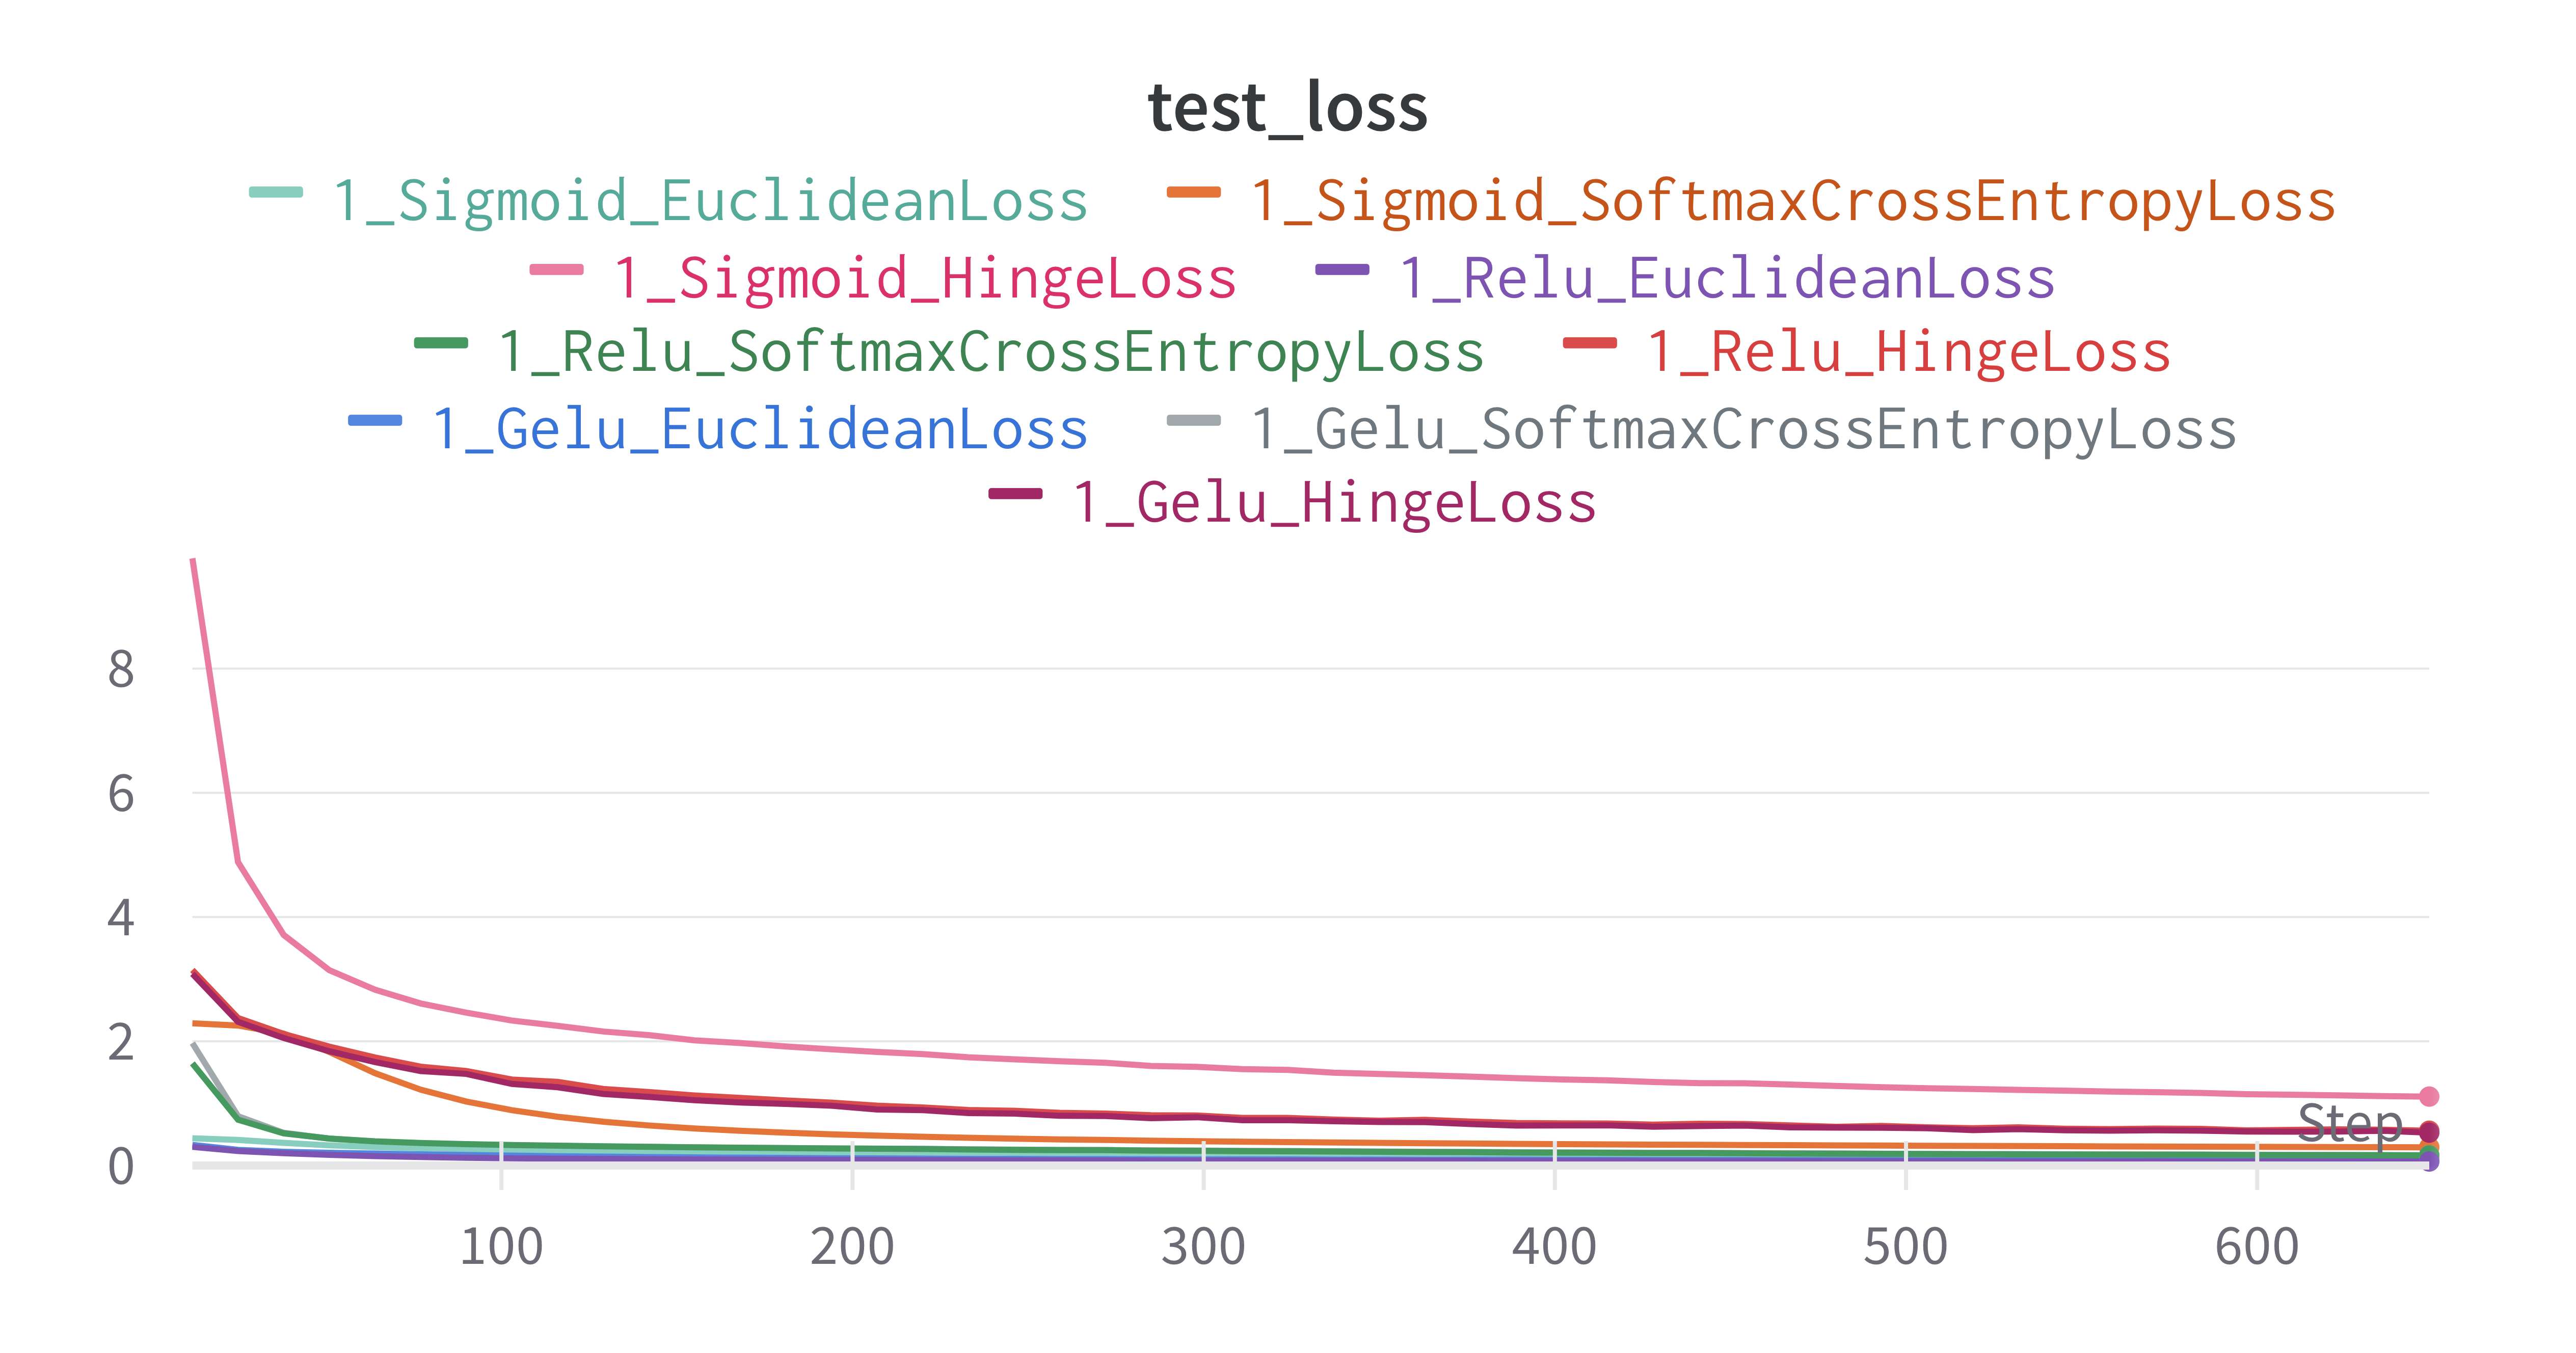
\includegraphics[width=1\textwidth]{../pics/单层实验-test_loss.png}
		\caption{单隐藏层实验 test loss}
	\end{subfigure}
	\begin{subfigure}{0.475\textwidth}
		\centering
		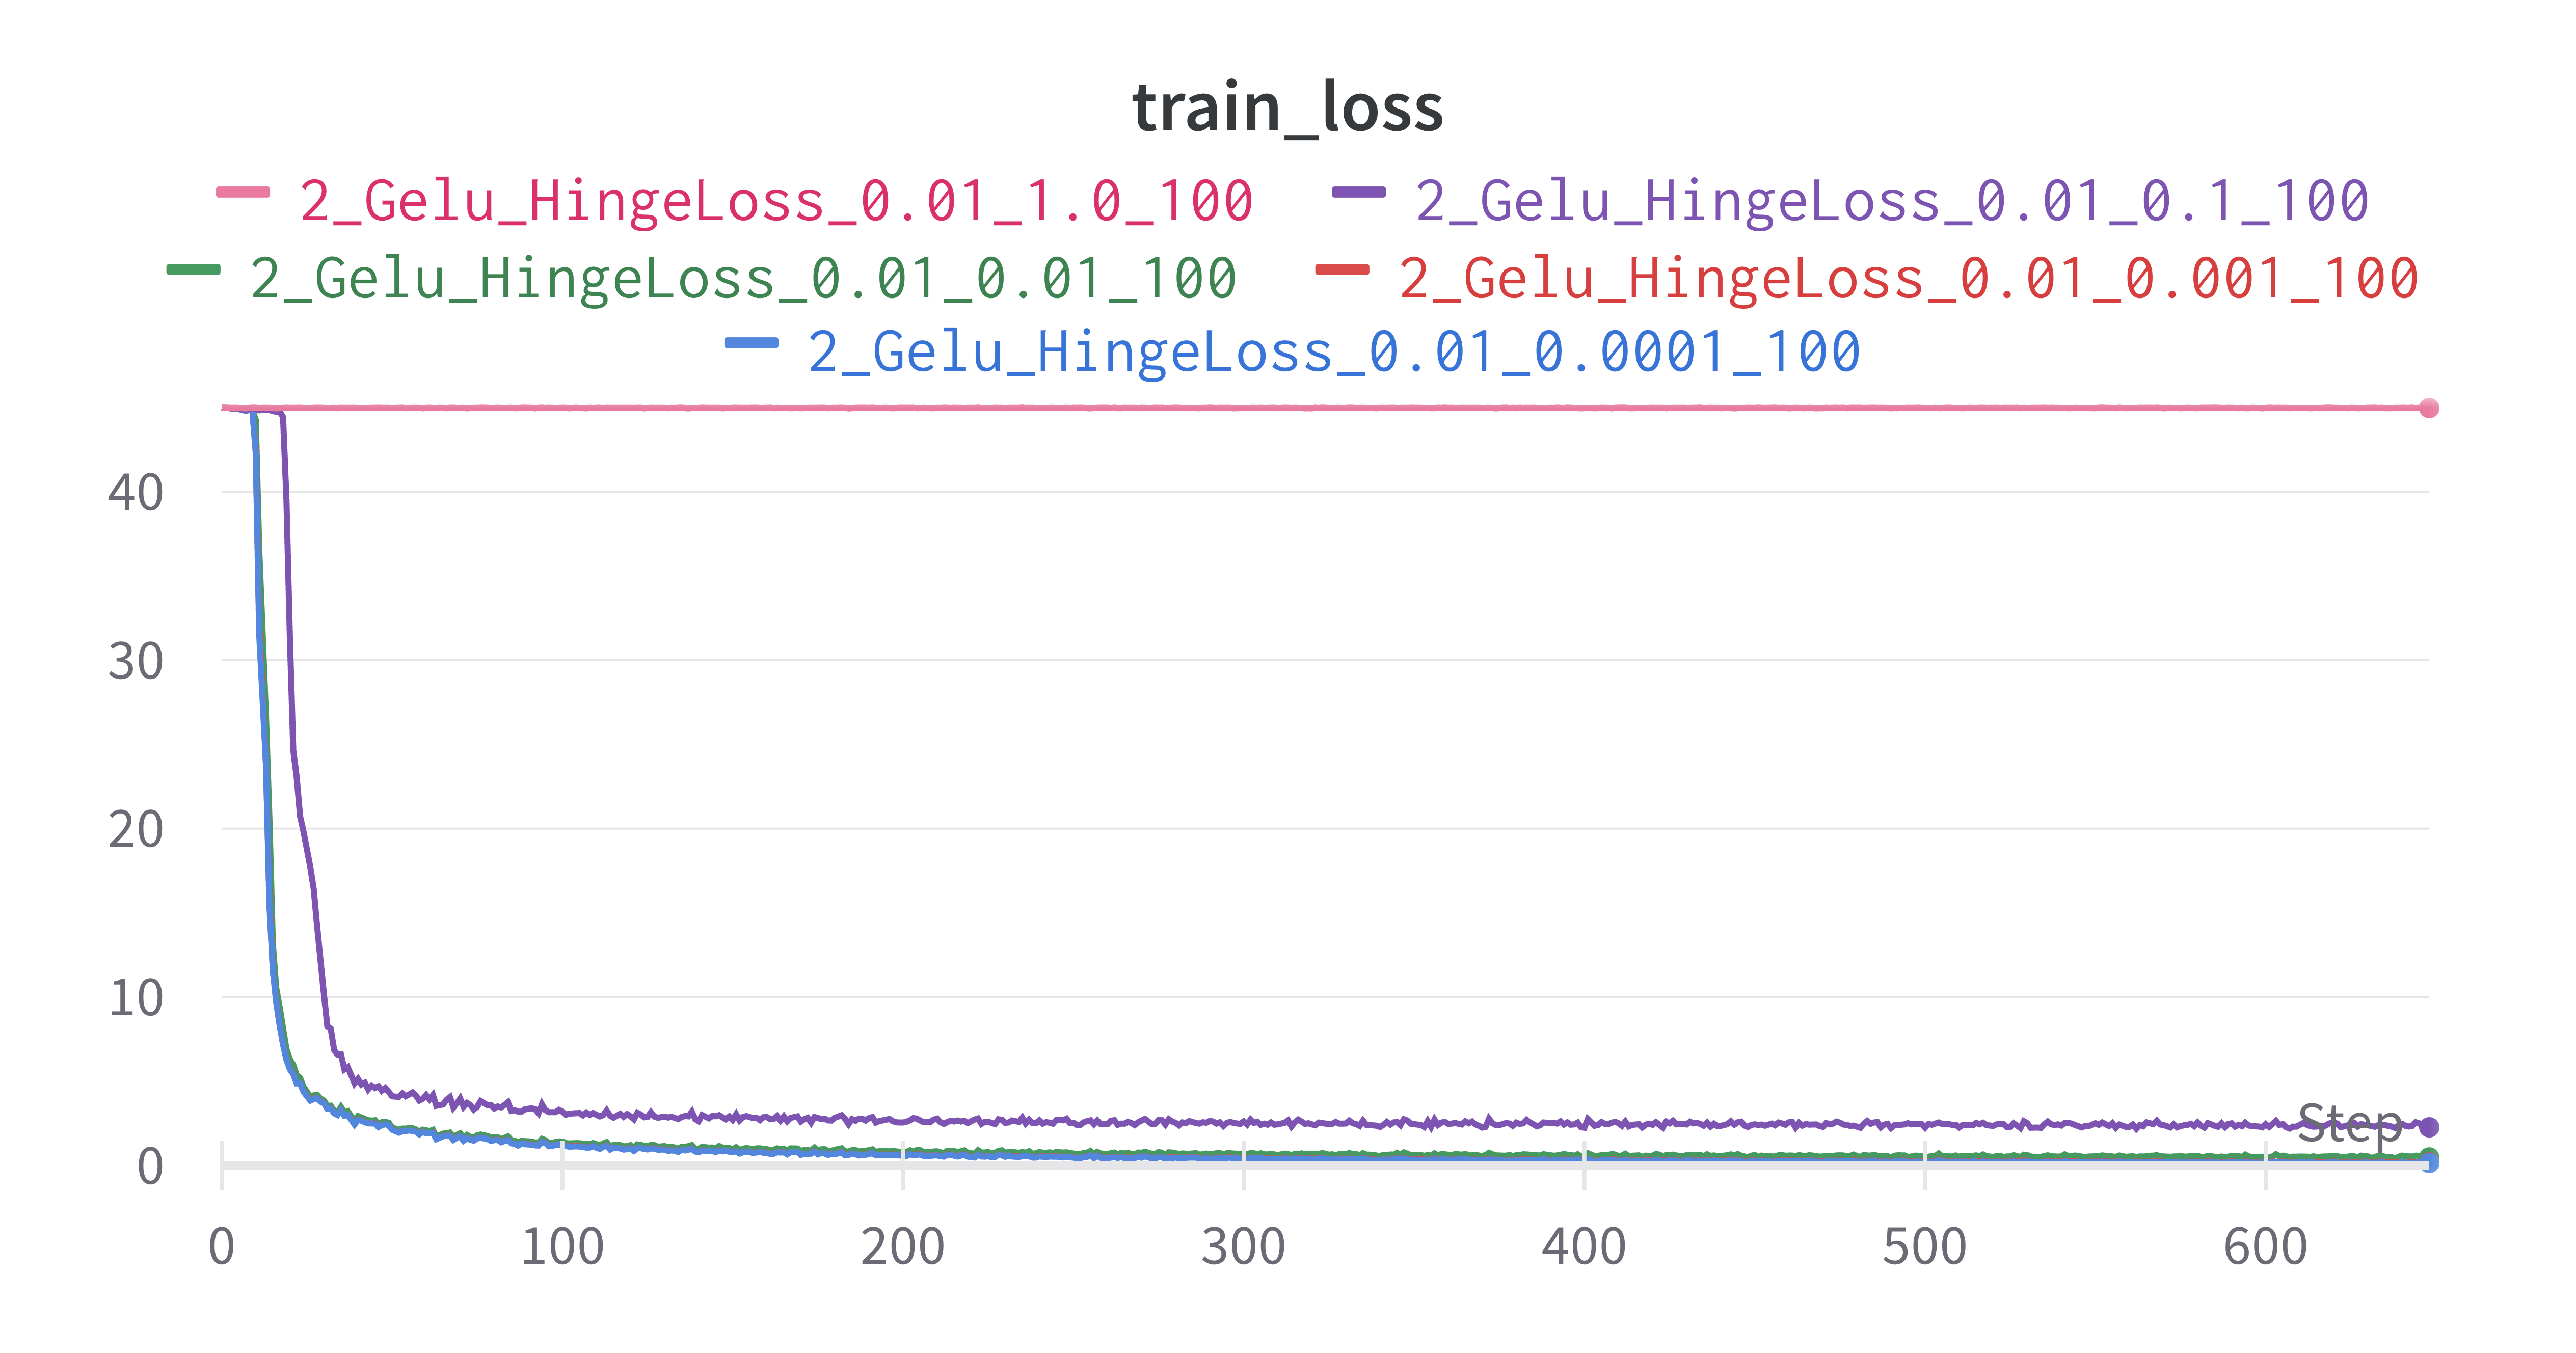
\includegraphics[width=1\textwidth]{../pics/消减率_2_Gelu_HingeLoss_train_loss.png}
		\caption{单隐藏层实验 test accuracy}
	\end{subfigure}
\caption{图例说明}
\label{fig:1}
\end{figure}

\subsection{零隐藏层实验}

对于零隐藏层网络,分别使用三种损失函数,训练过程和训练结果如图 ~\ref{fig:2} 所示。可以发现如果只有一层线性层的话,没有隐藏层,则无法达到预期的学习效果。

\begin{figure}[htbp]
	\centering
	\begin{subfigure}{0.475\textwidth}
		\centering
		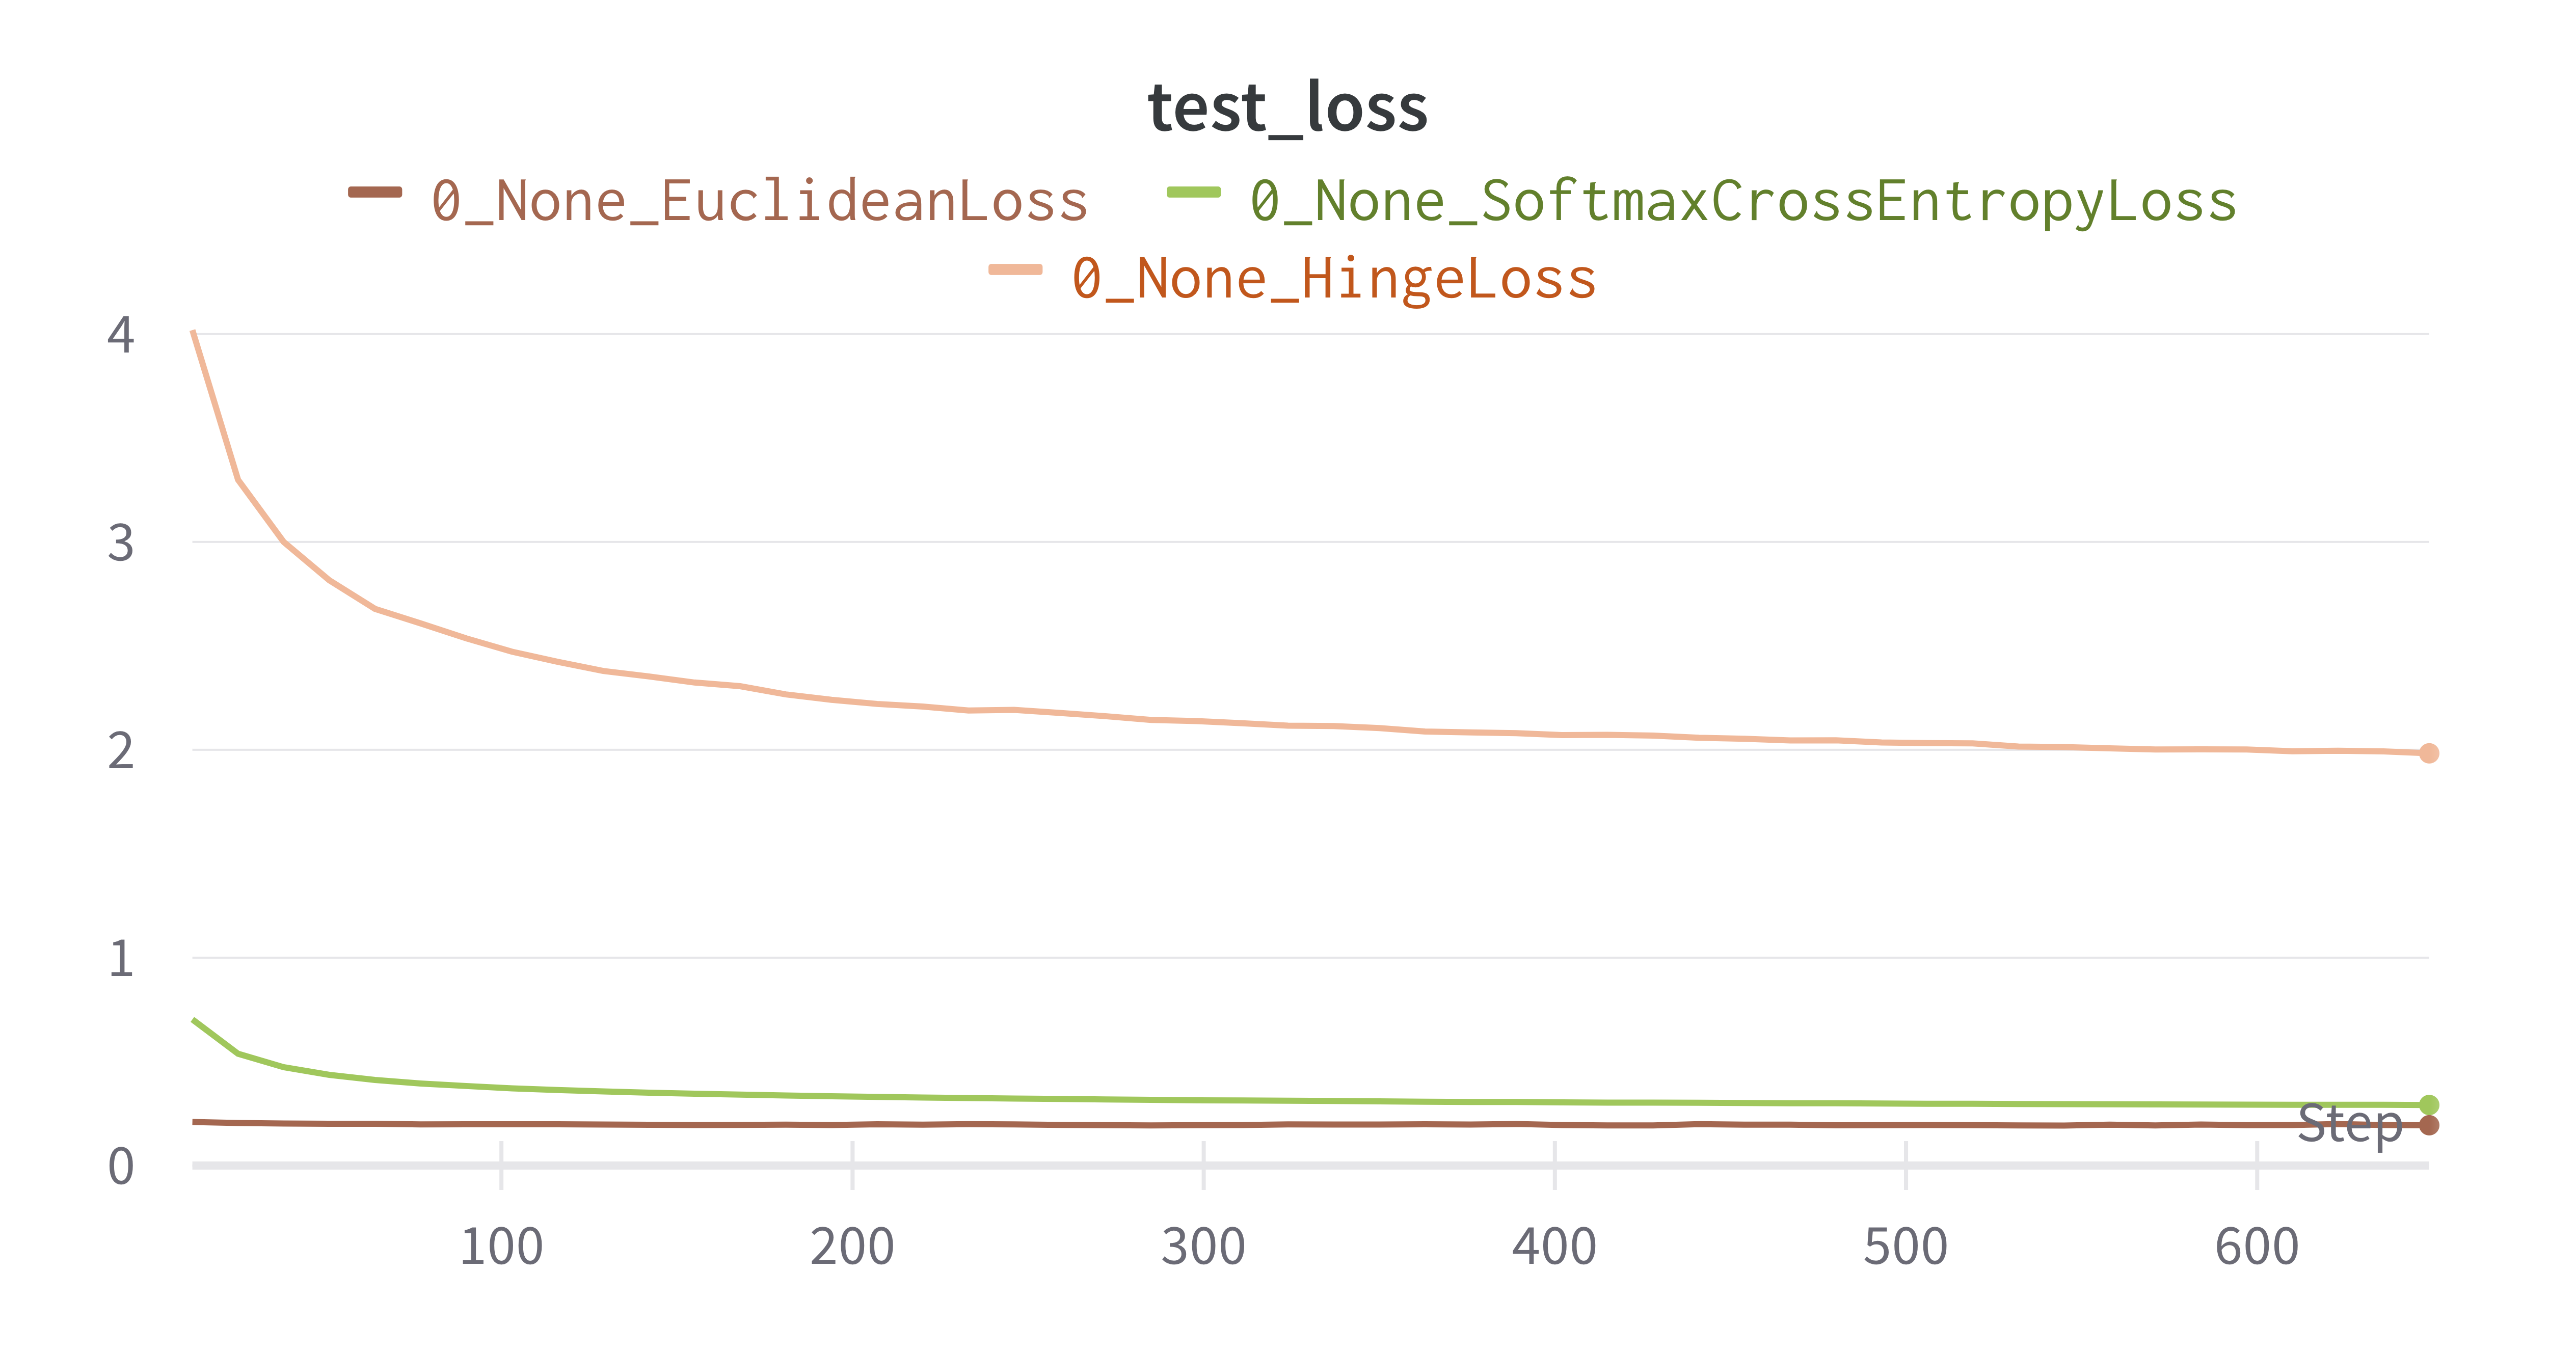
\includegraphics[width=1\textwidth]{../pics/零层实验-test-loss.png}
		\caption{零隐藏层 test loss}
	\end{subfigure}
	\begin{subfigure}{0.475\textwidth}
		\centering
		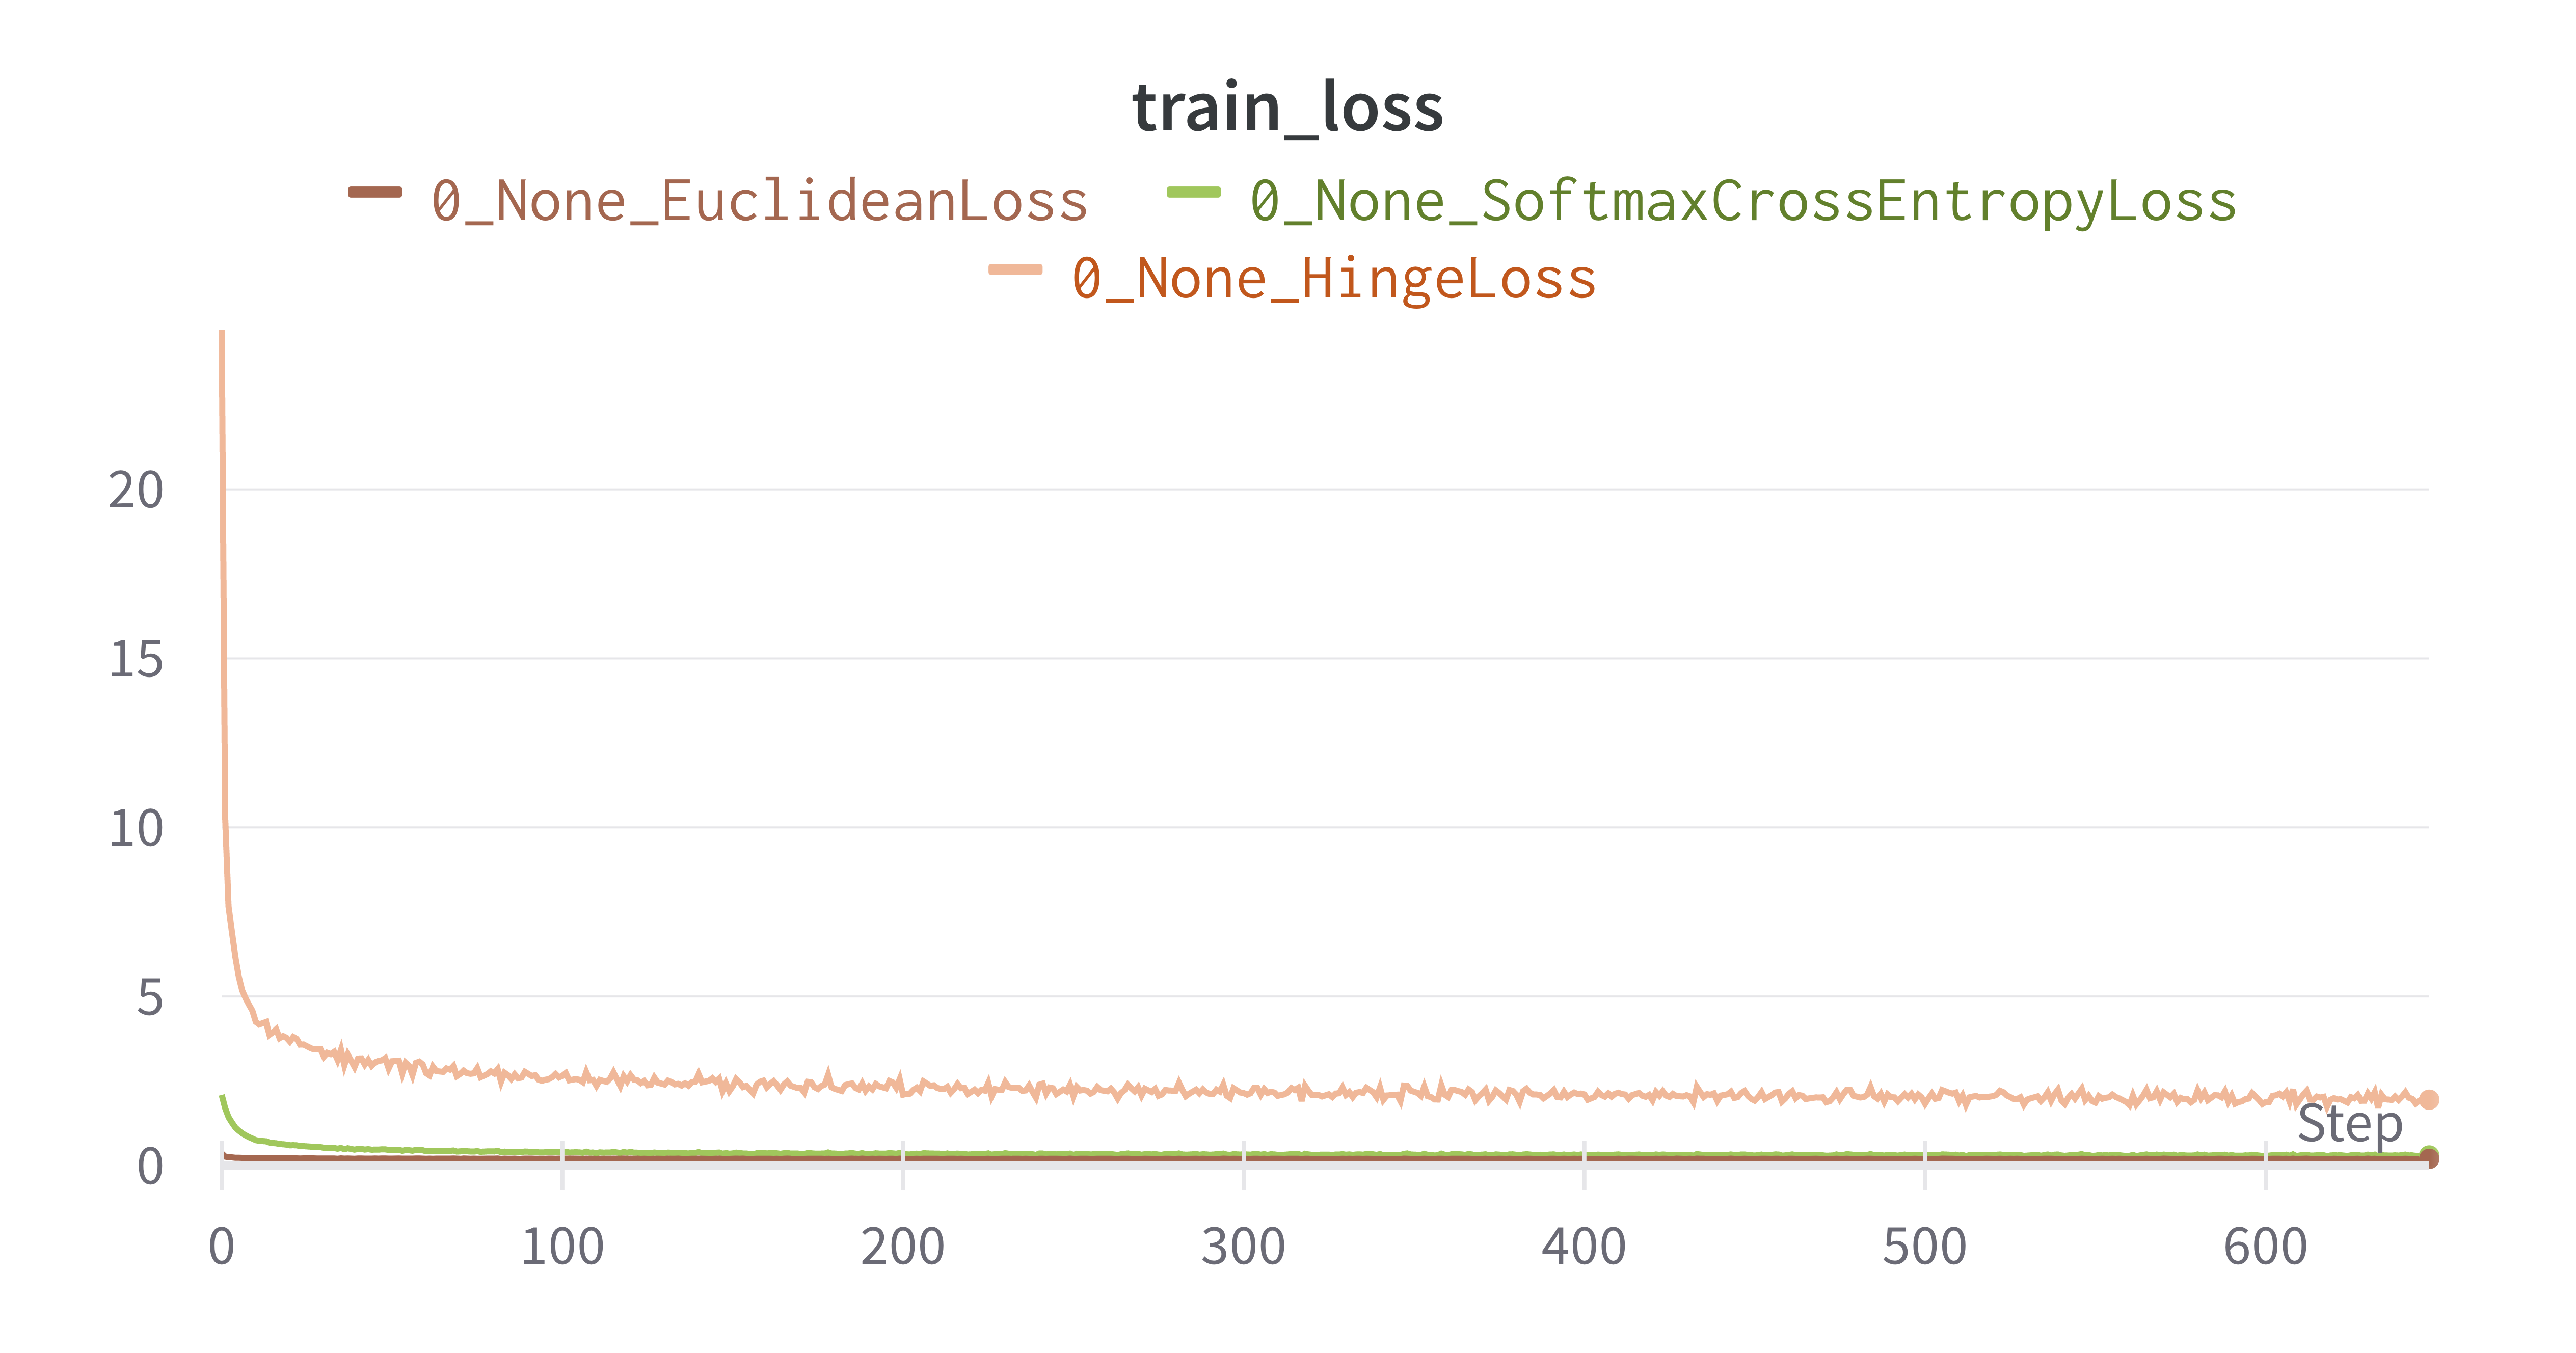
\includegraphics[width=1\textwidth]{../pics/零层实验-train-loss.png}
		\caption{零隐藏层 train loss}
	\end{subfigure}
	\begin{subfigure}{0.475\textwidth}
		\centering
		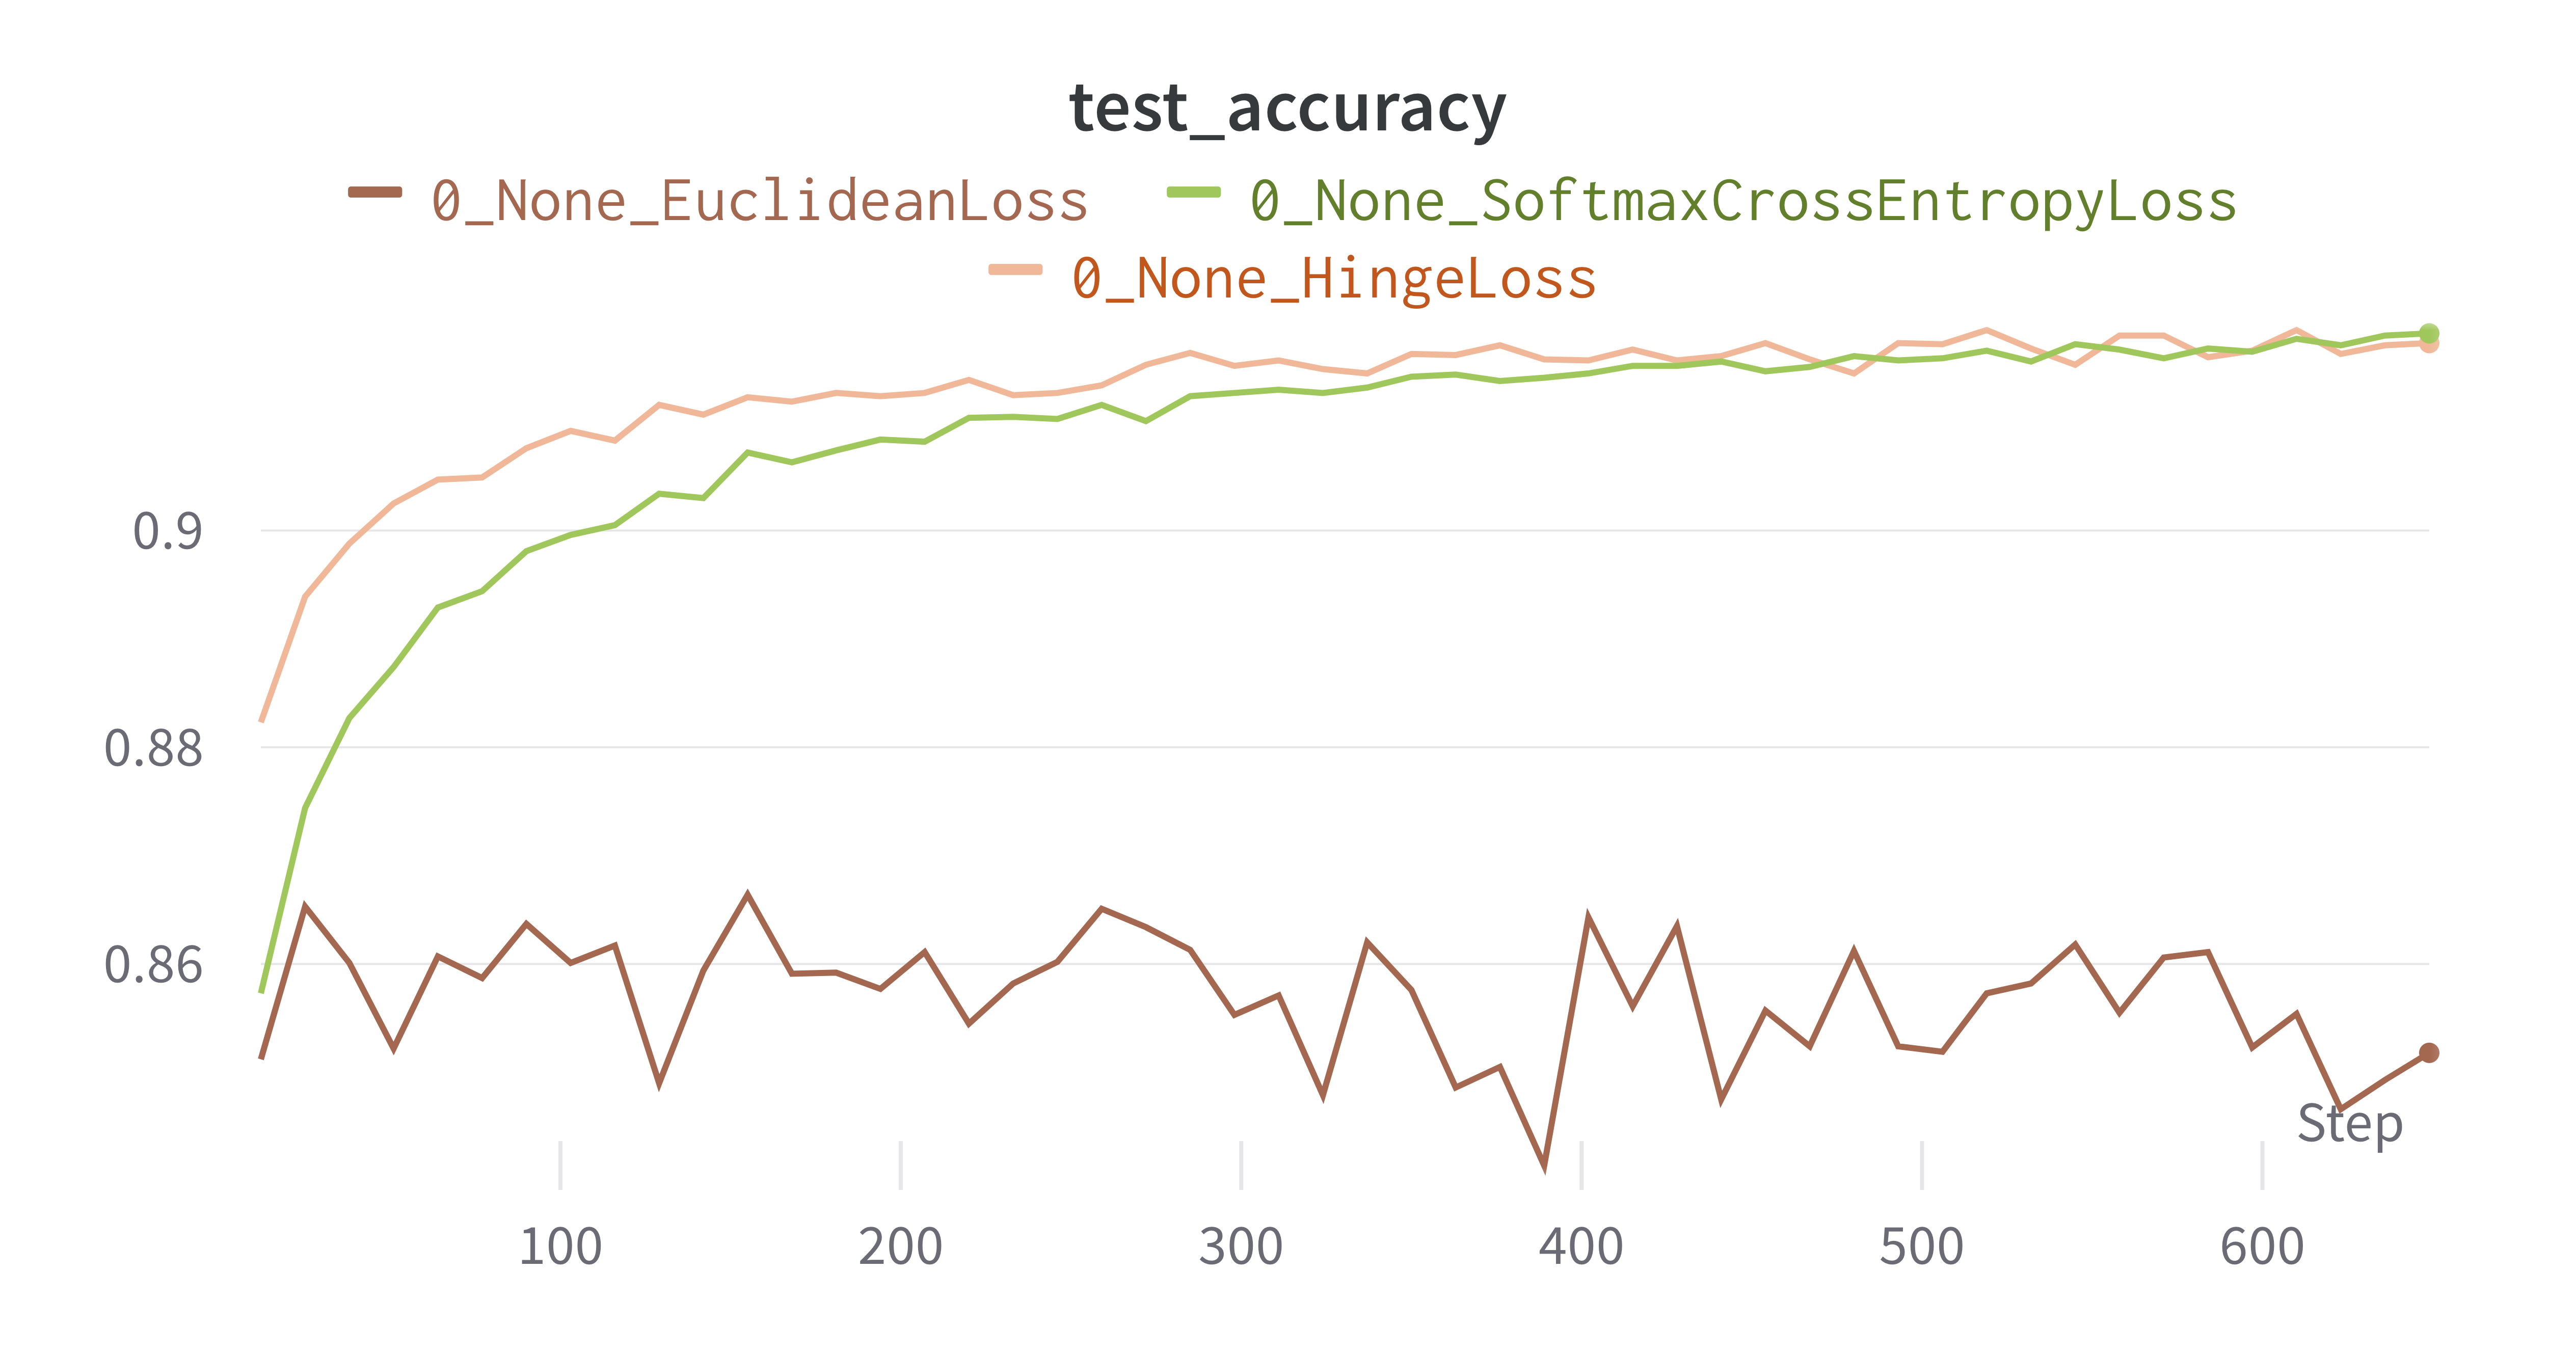
\includegraphics[width=1\textwidth]{../pics/零层实验-test-acc.png}
		\caption{零隐藏层 test accuracy}
	\end{subfigure}
	\begin{subfigure}{0.475\textwidth}
		\centering
		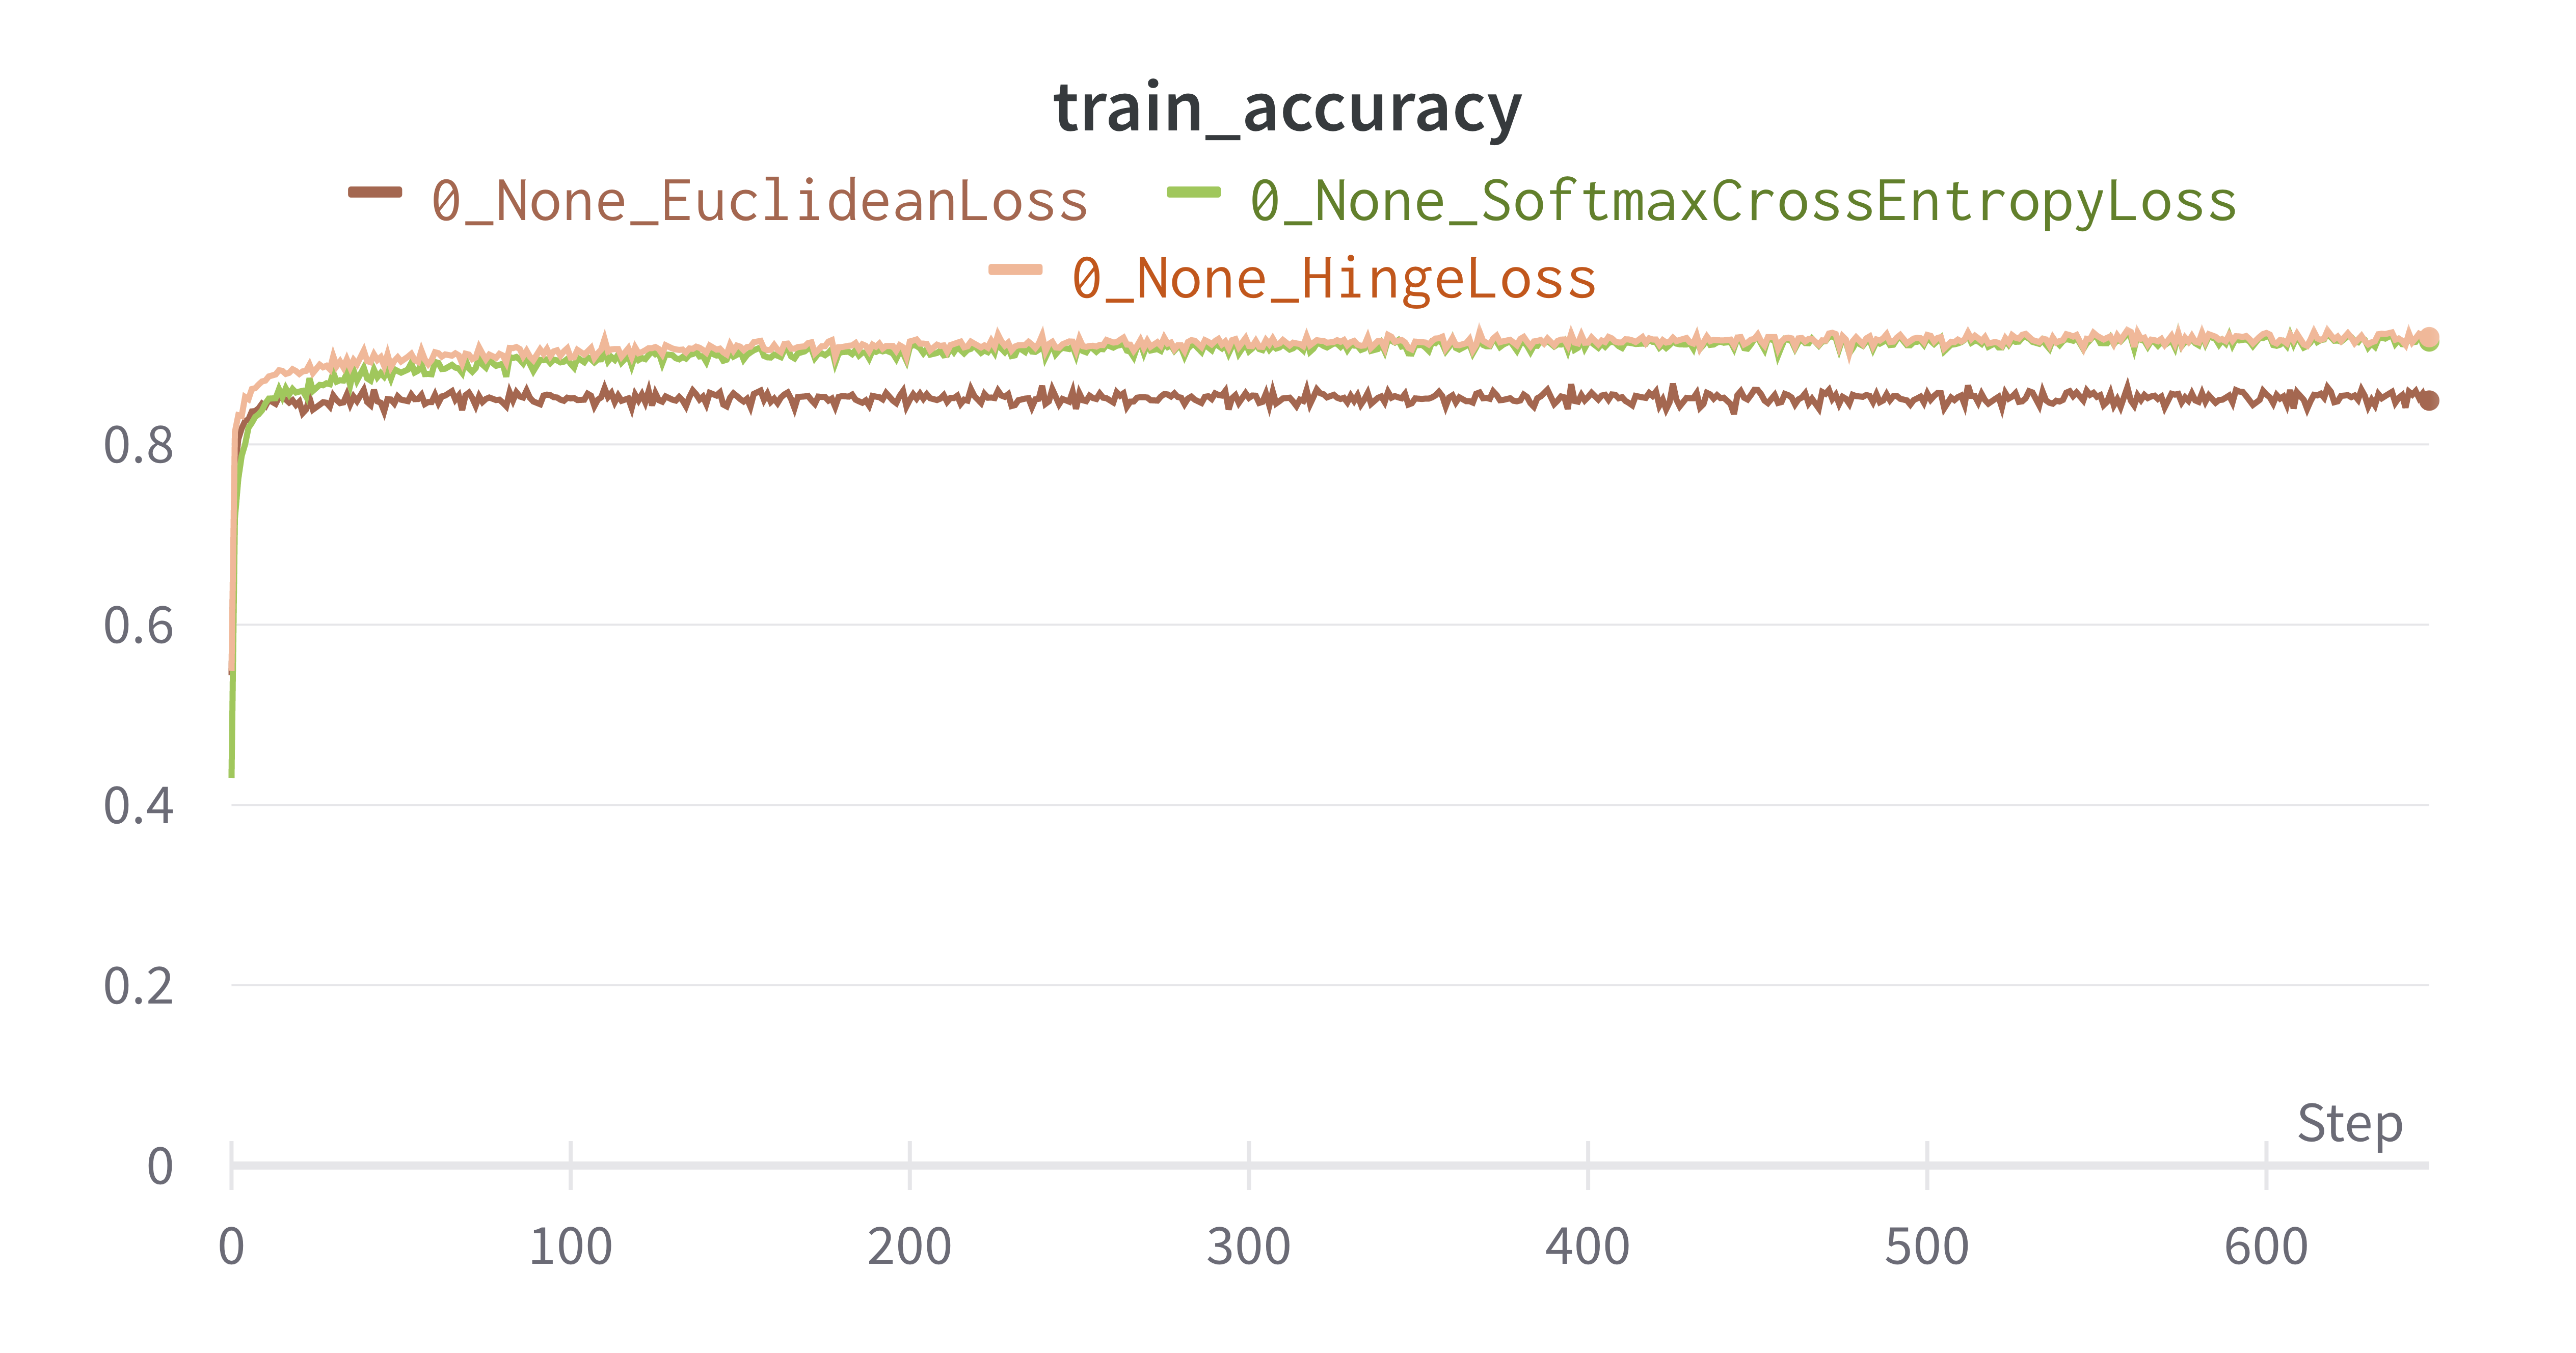
\includegraphics[width=1\textwidth]{../pics/零层实验-train_acc.png}
		\caption{零隐藏层 train accuracy}
	\end{subfigure}
	\caption{零隐藏层实验效果}
	\label{fig:2}
\end{figure}

\subsection{单隐藏层实验}
增加单层隐藏层,隐藏层神经元数设置为 100,遍历三种损失函数和三种激活函数进行对比实验。其结果如图 \ref{fig:3} 所示。

\begin{figure}[htbp]
	\centering
	\begin{subfigure}{0.475\textwidth}
		\centering
		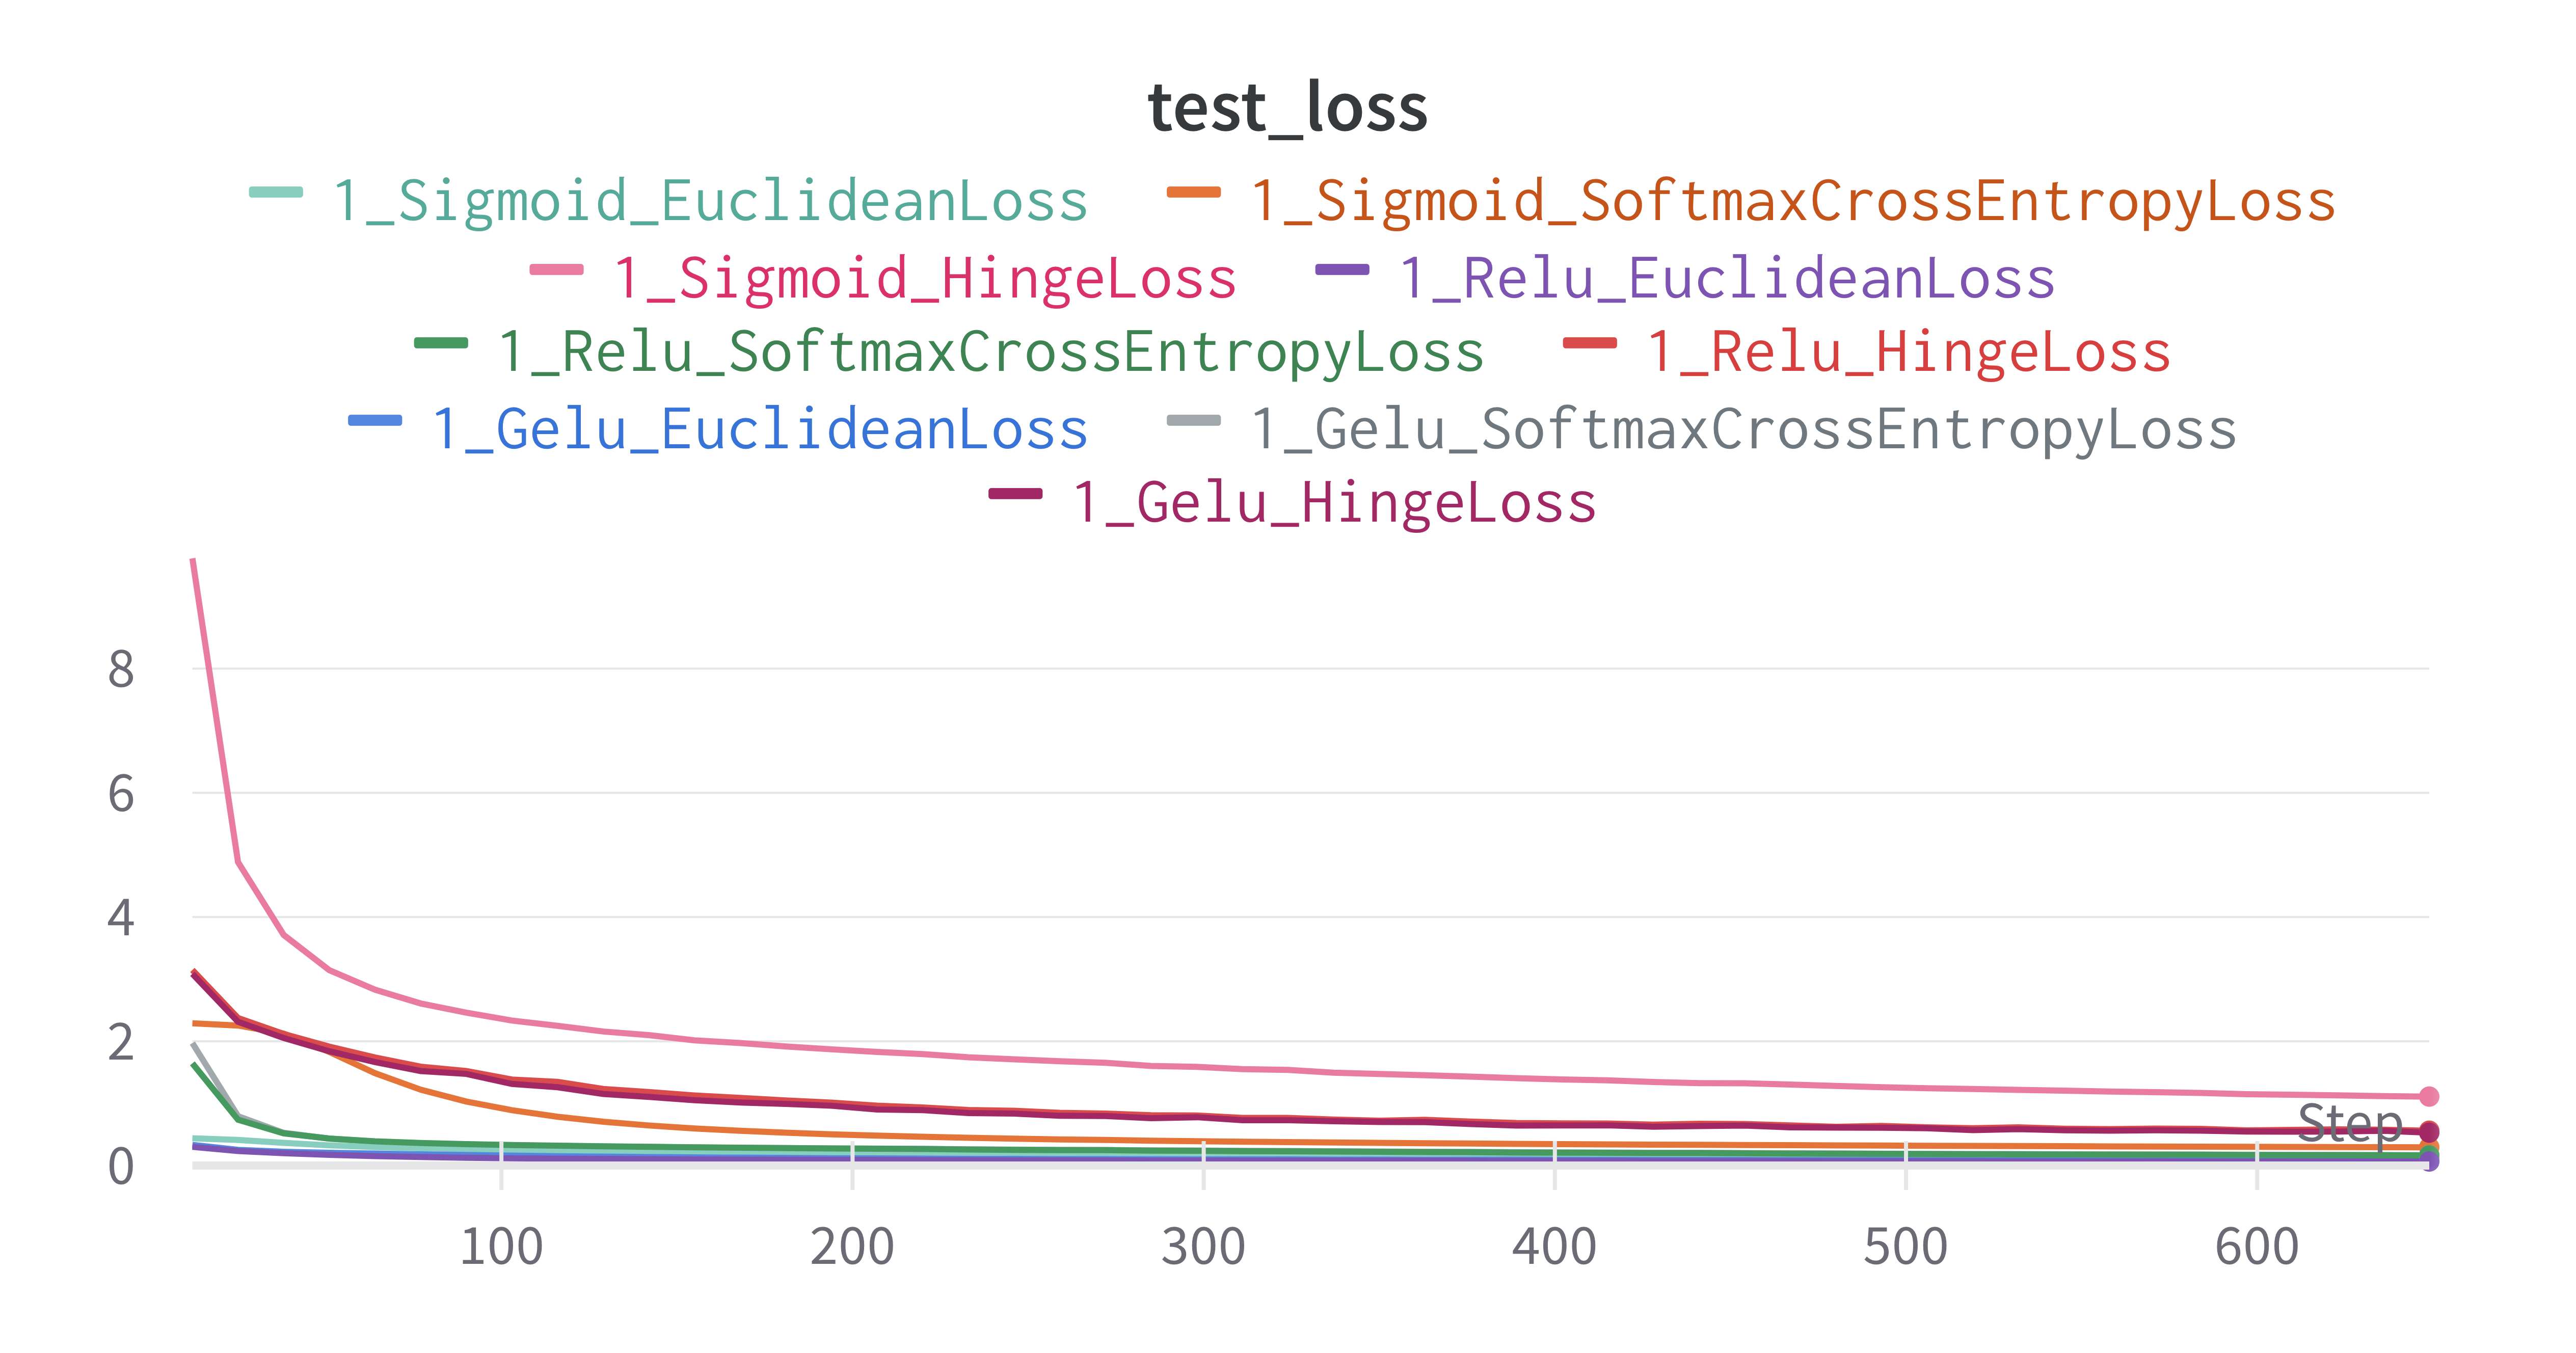
\includegraphics[width=1\textwidth]{../pics/单层实验-test_loss.png}
		\caption{单隐藏层 test loss}
	\end{subfigure}
	\begin{subfigure}{0.475\textwidth}
		\centering
		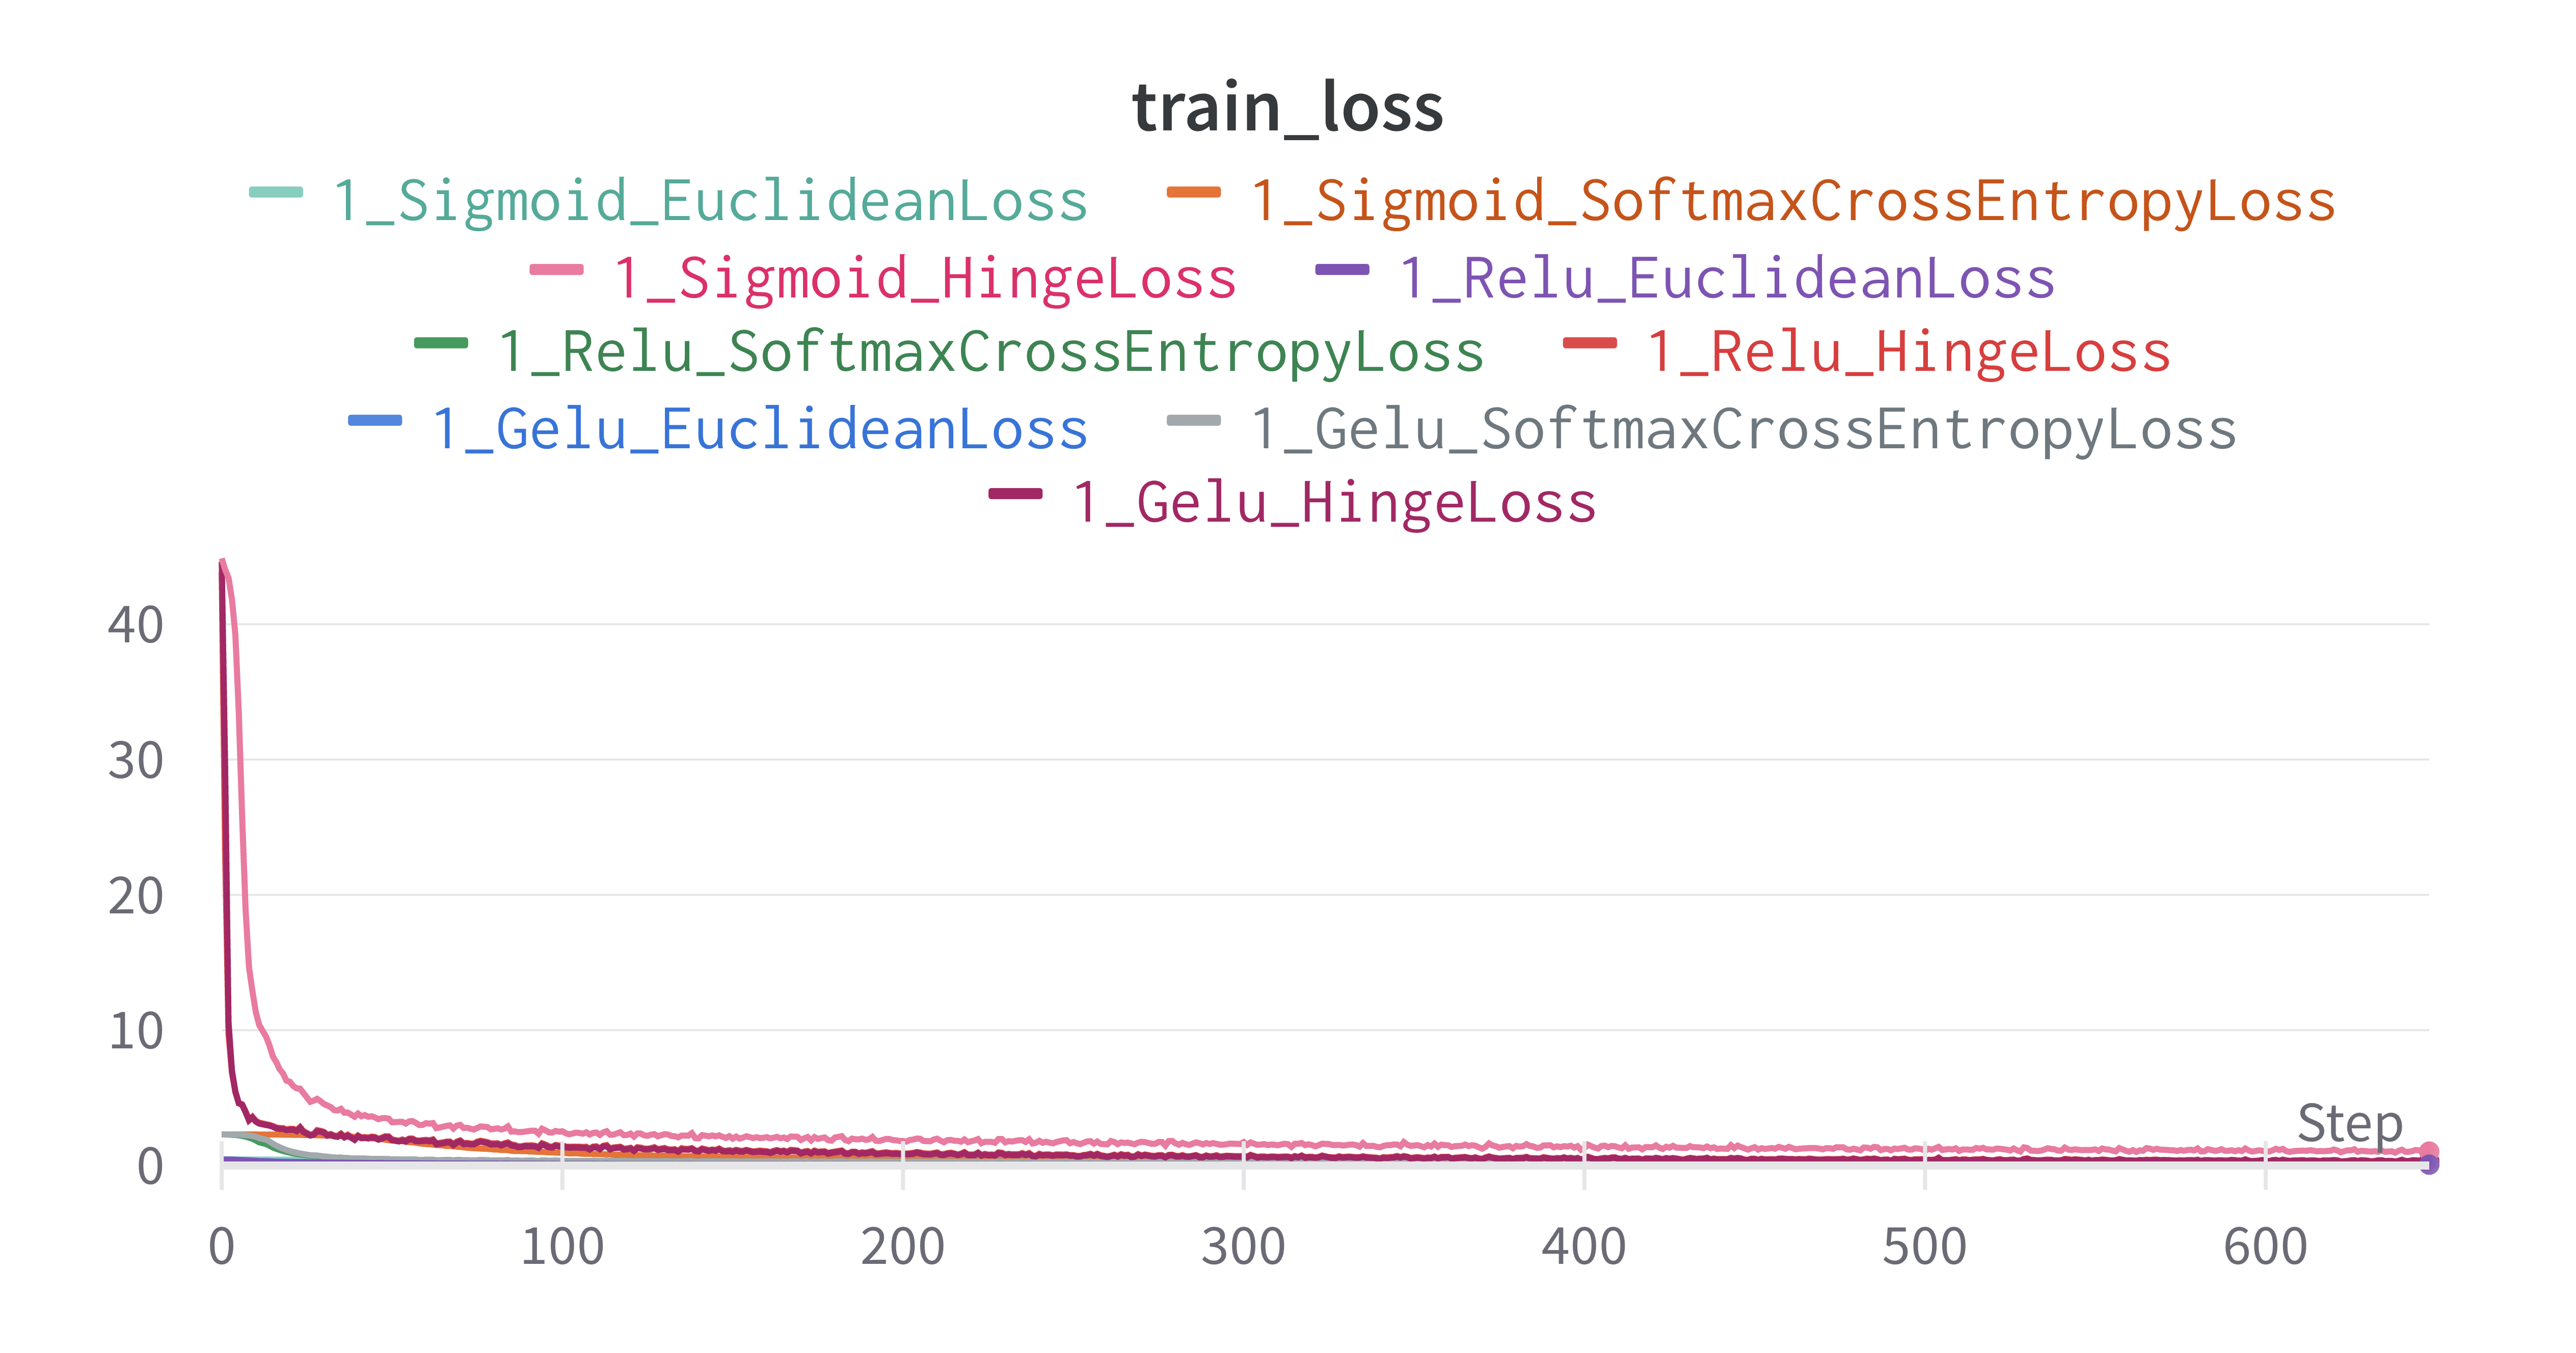
\includegraphics[width=1\textwidth]{../pics/单层实验-train_loss.png}
		\caption{单隐藏层 train loss}
	\end{subfigure}
	\begin{subfigure}{0.475\textwidth}
		\centering
		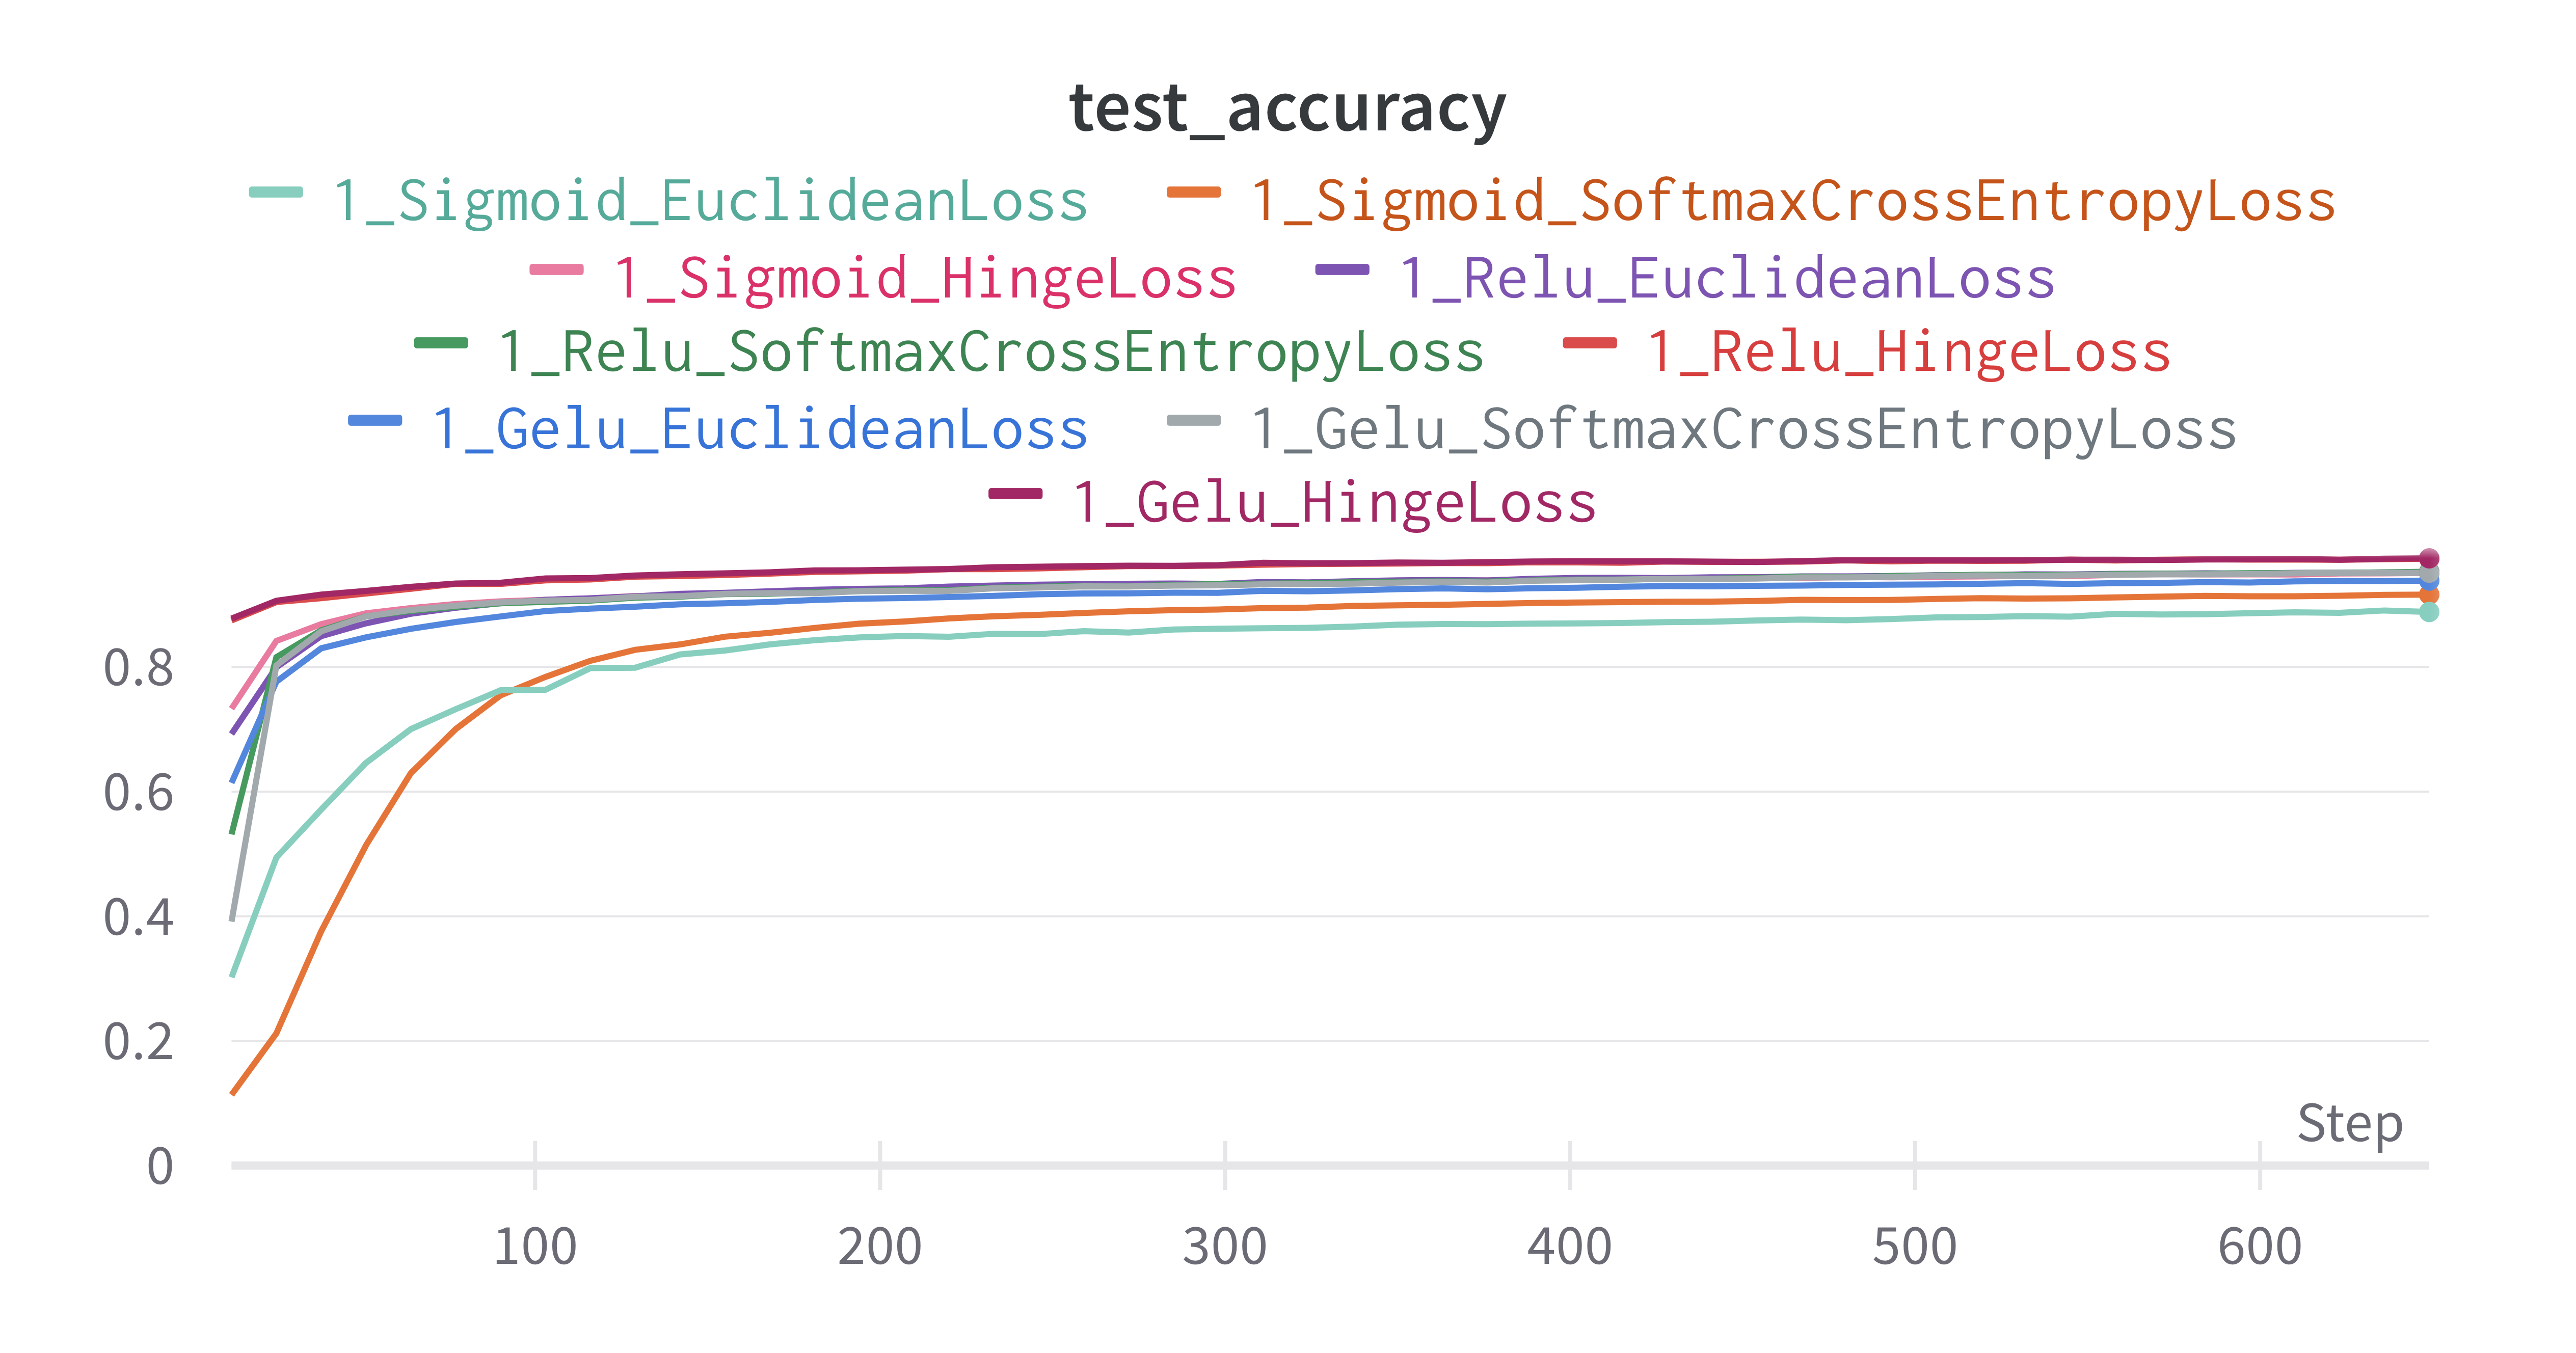
\includegraphics[width=1\textwidth]{../pics/单层实验-test_acc.png}
		\caption{单隐藏层 test accuracy}
	\end{subfigure}
	\begin{subfigure}{0.475\textwidth}
		\centering
		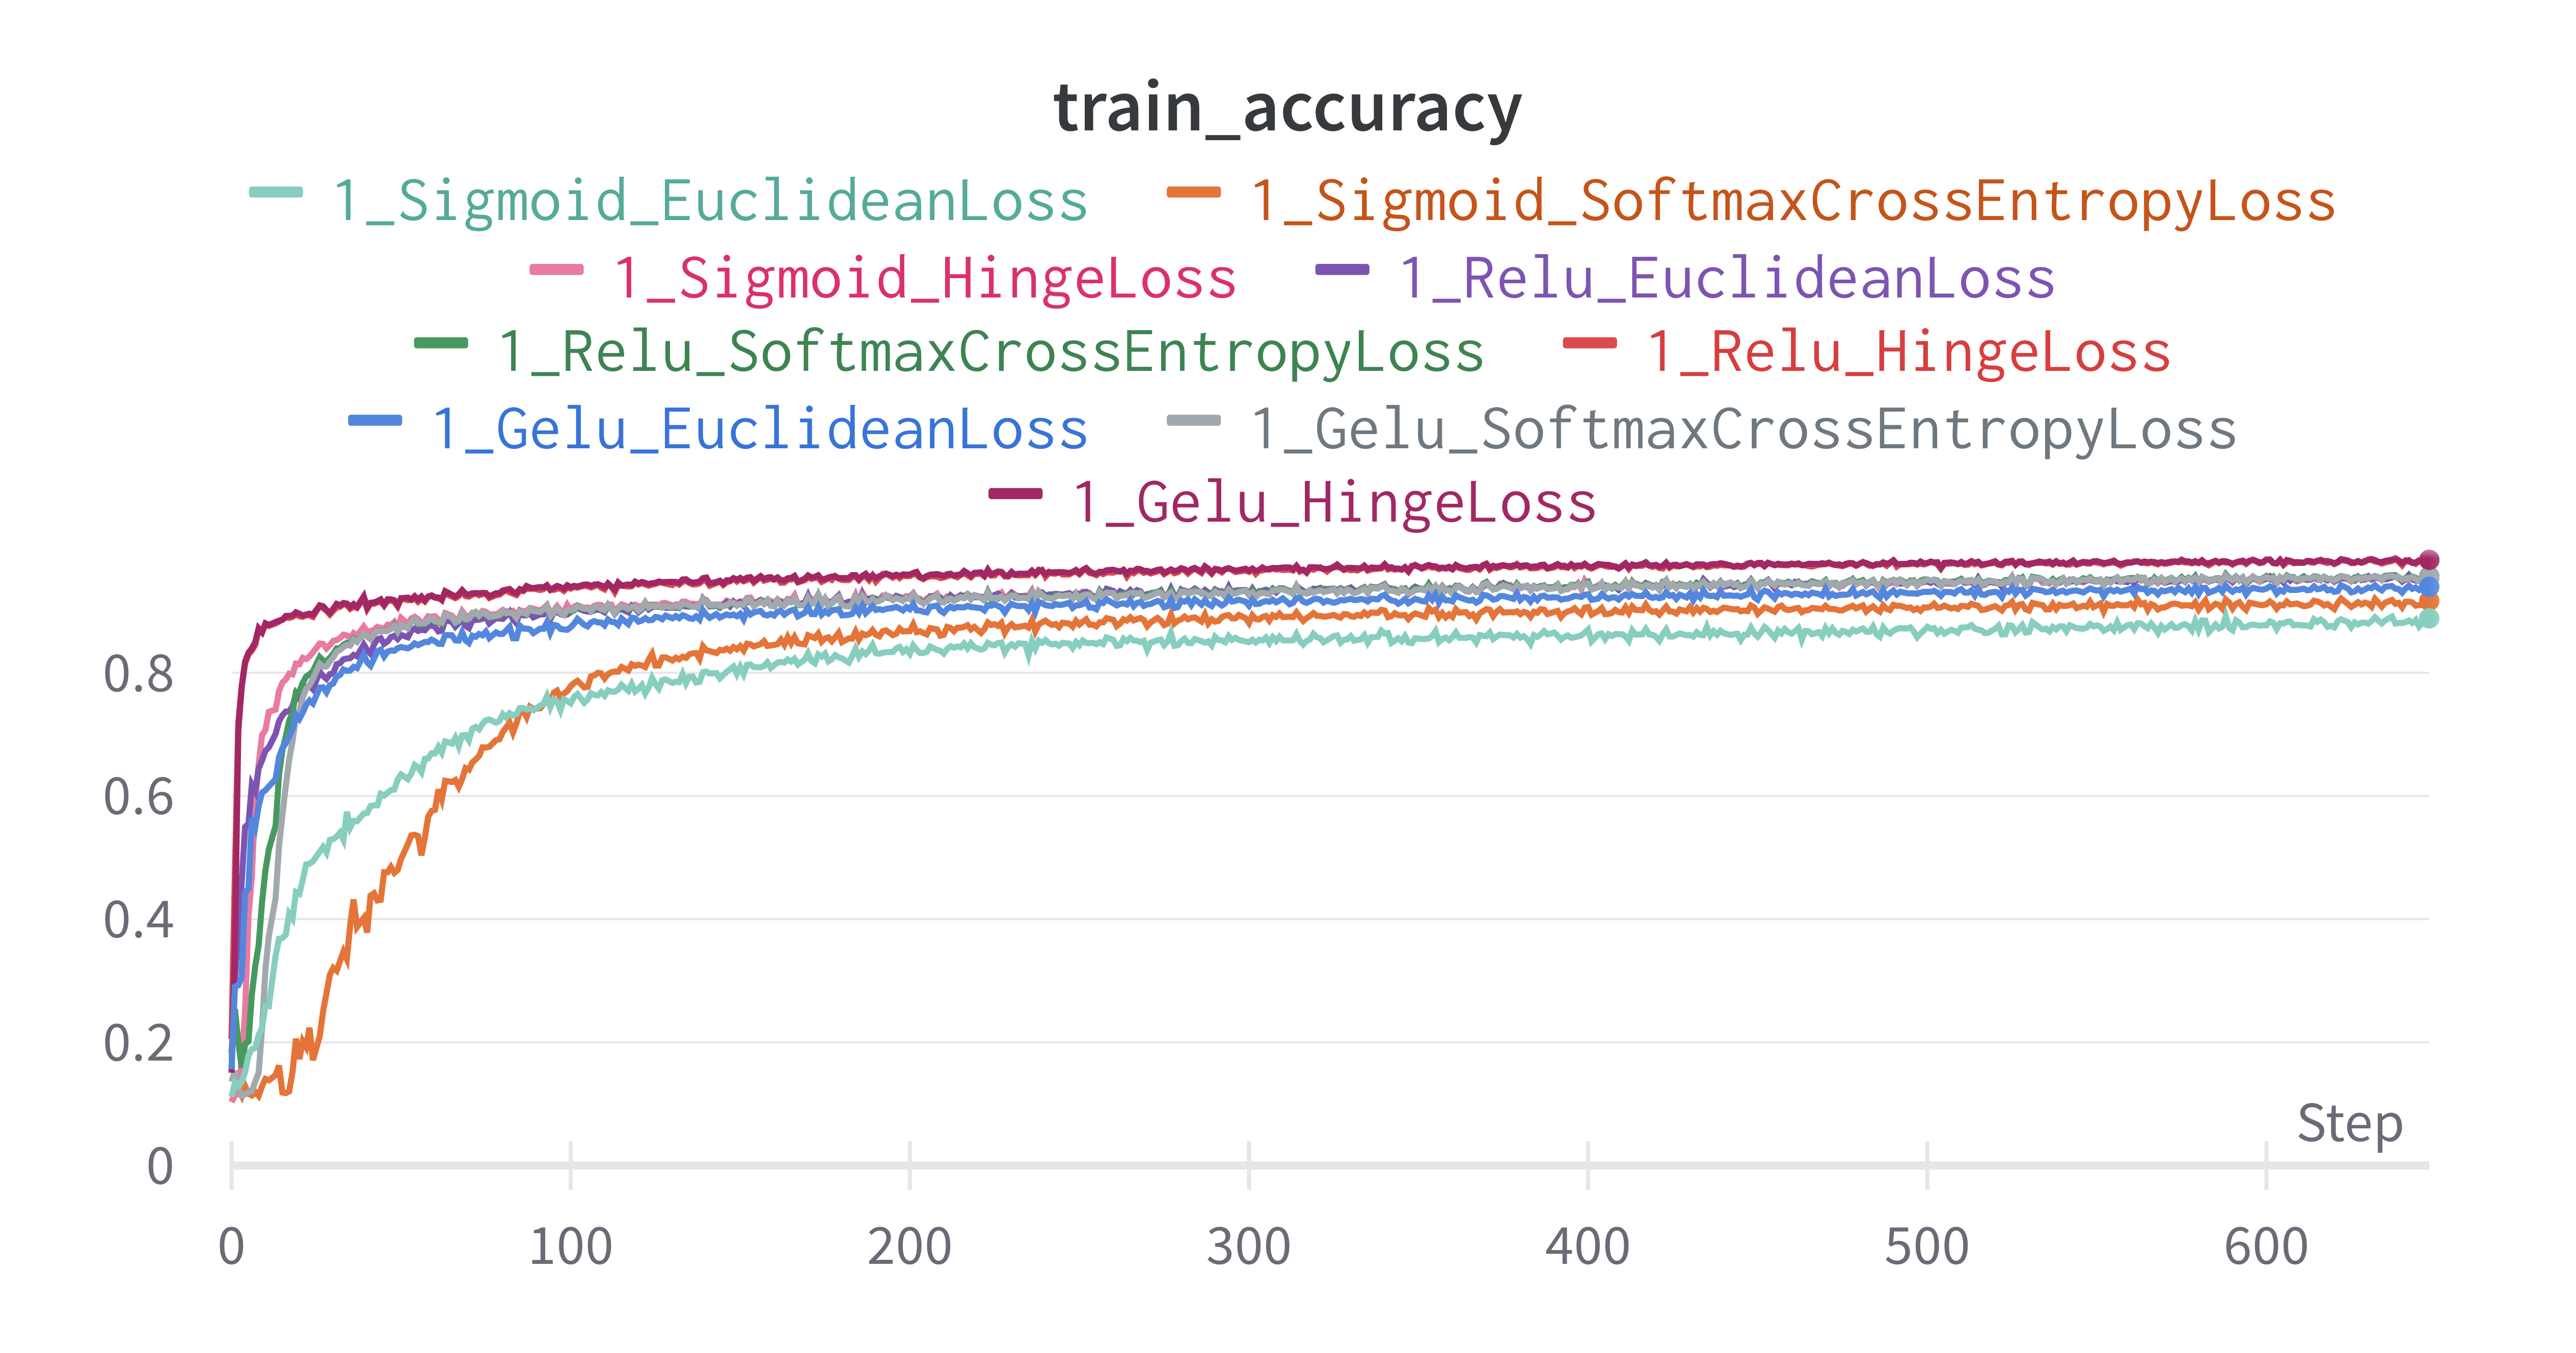
\includegraphics[width=1\textwidth]{../pics/单层实验-train_acc.png}
		\caption{单隐藏层 train accuracy}
	\end{subfigure}
	\caption{单隐藏层实验效果}
	\label{fig:3}
\end{figure}

\subsubsection{不同损失函数对比}

在单隐藏层的前提下,固定激活函数为 Sigmoid,遍历三种损失函数,结果如图 \ref{fig:4} 所示。\\
分析结果可以发现,(1)就准确率而言,在测试集和训练集上均是 Hinge 效果最好而 Euclidean 效果最差;(2)就损失值而言,Hinge、SoftmaxCrossEntropy 和 Euclidean 计算出的绝对值存在着明显的差异,损失值无法横向比较,然而对比损失值下降速度,能够观察到 Hinge 收敛效果与收敛速度最为显著;(3)就收敛速度而言,Hinge 收敛曲线斜率最高,收敛最快,而 Euclidean 收敛最慢;(4)就训练时间而言,Hinge 耗时为 
29s,Euclidean 耗时也为 29s,SoftmaxCrossEntropy 耗时为 31s,三者并无显著差异。

\begin{figure}[htbp]
	\centering
	\begin{subfigure}{0.475\textwidth}
		\centering
		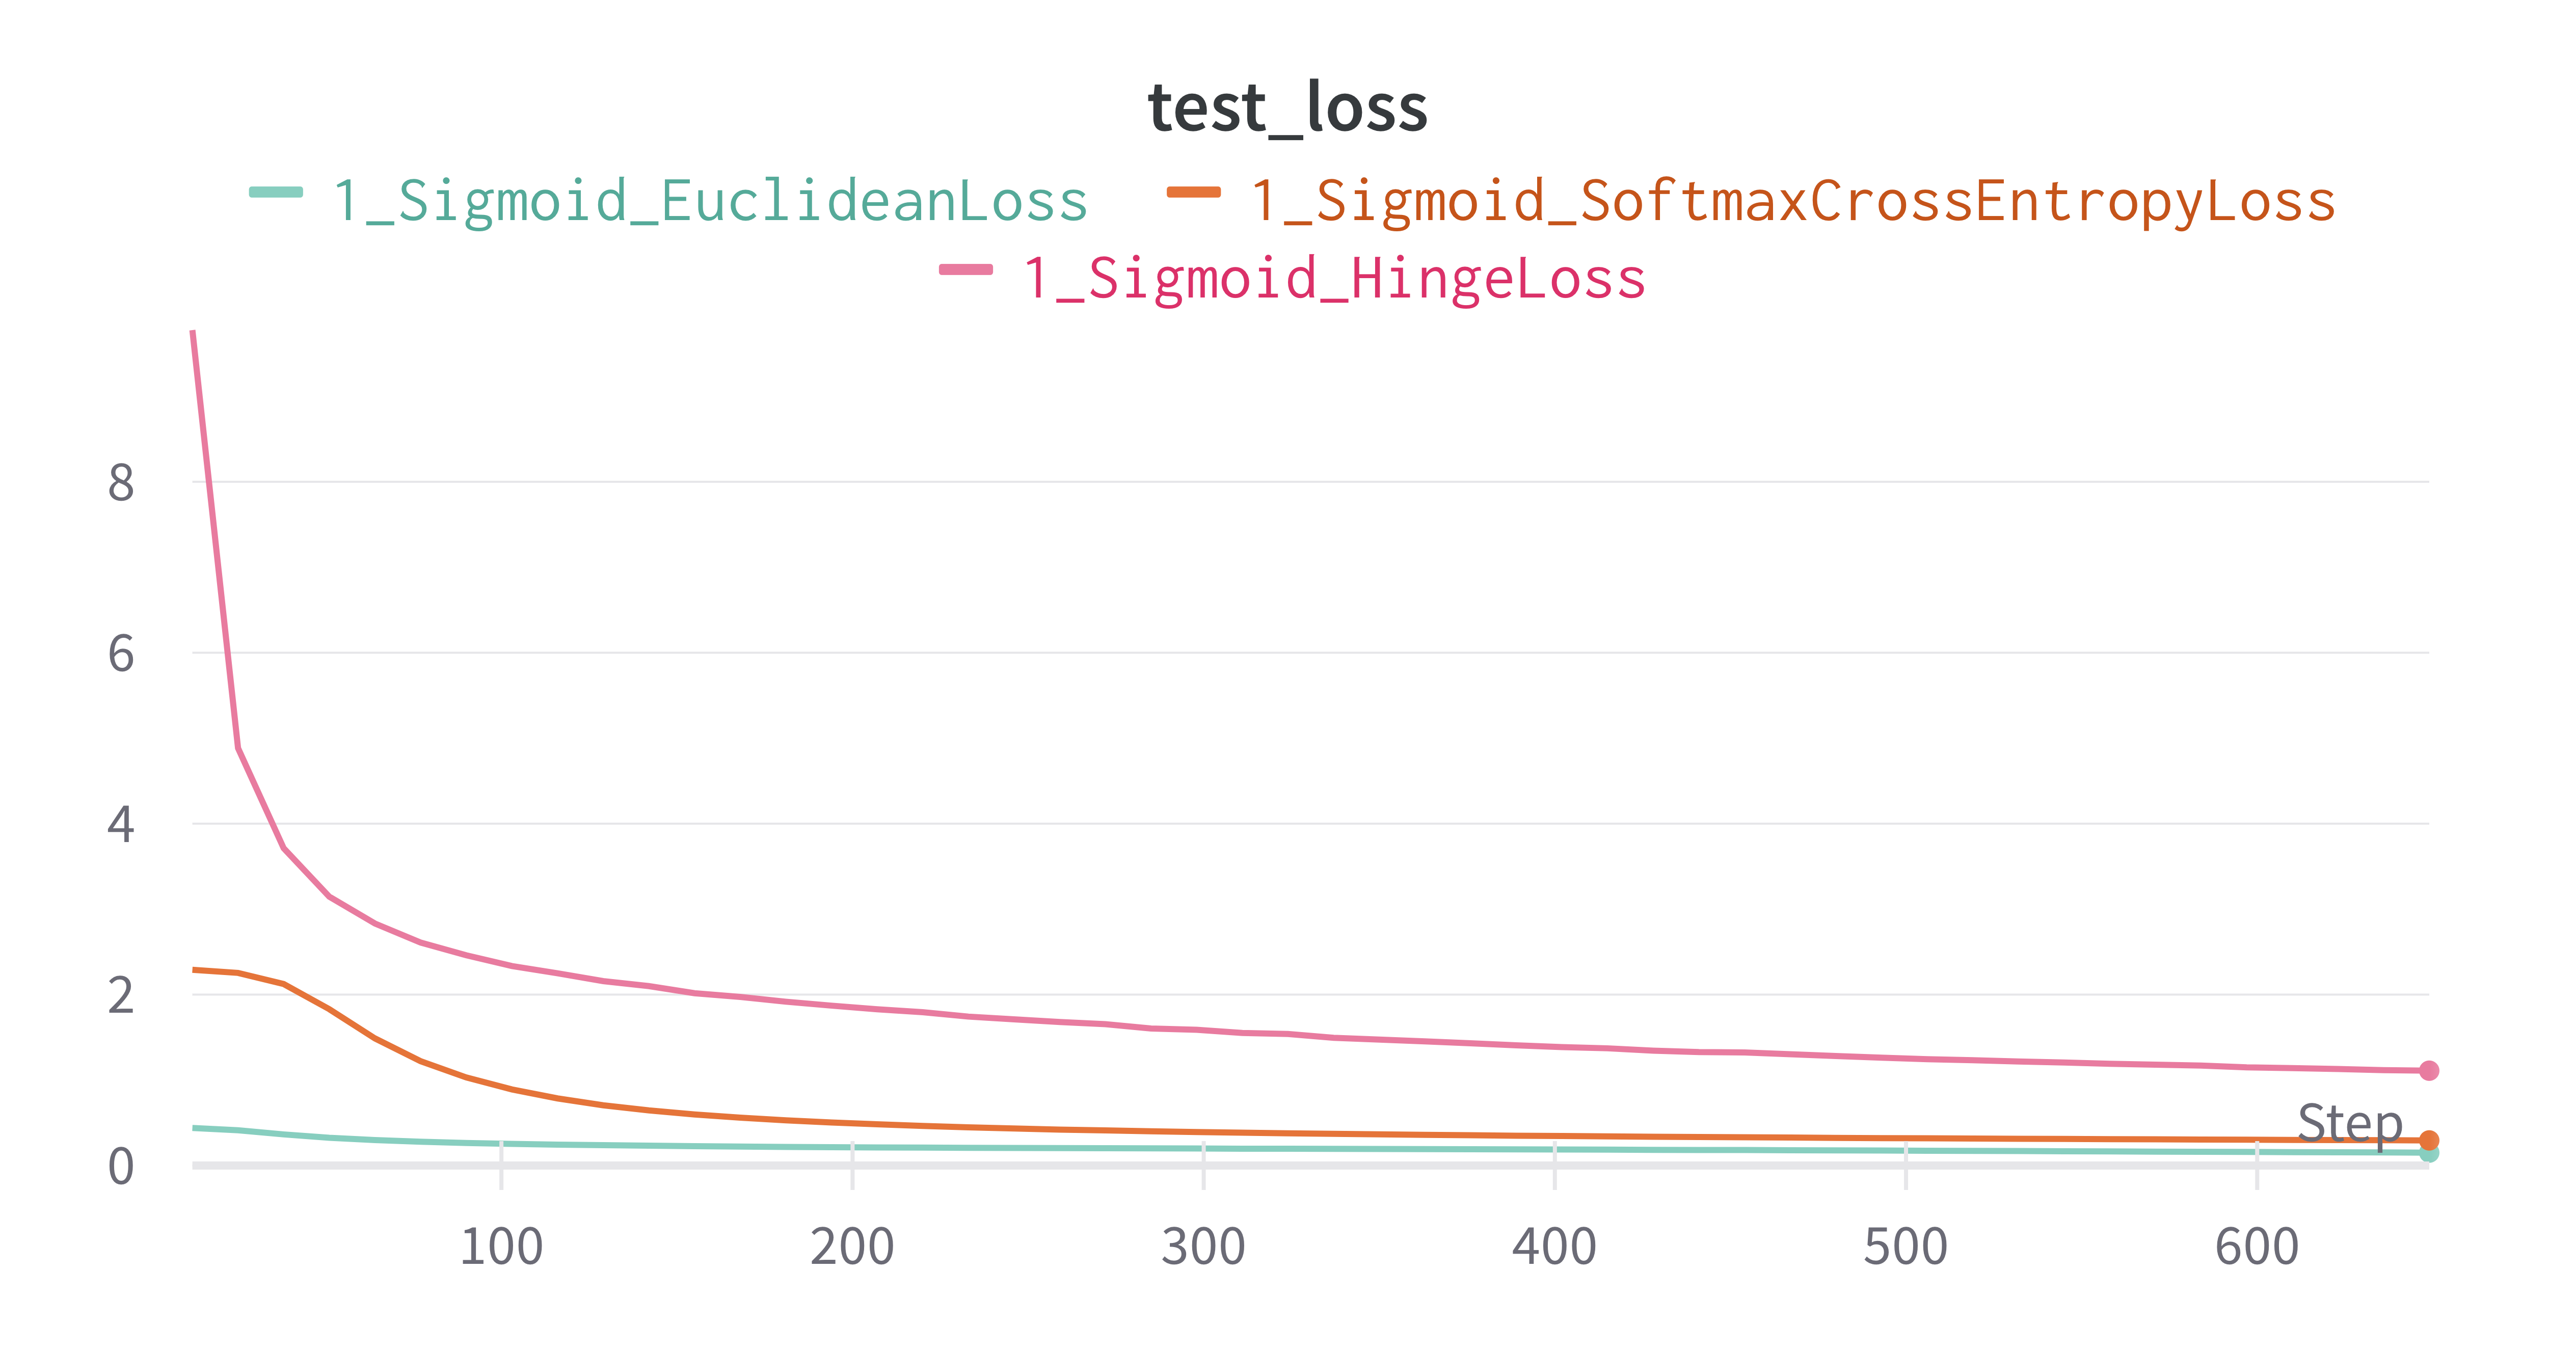
\includegraphics[width=1\textwidth]{../pics/单层损失函数test_loss.png}
		\caption{单隐藏层遍历损失函数对比 test loss}
	\end{subfigure}
	\begin{subfigure}{0.475\textwidth}
		\centering
		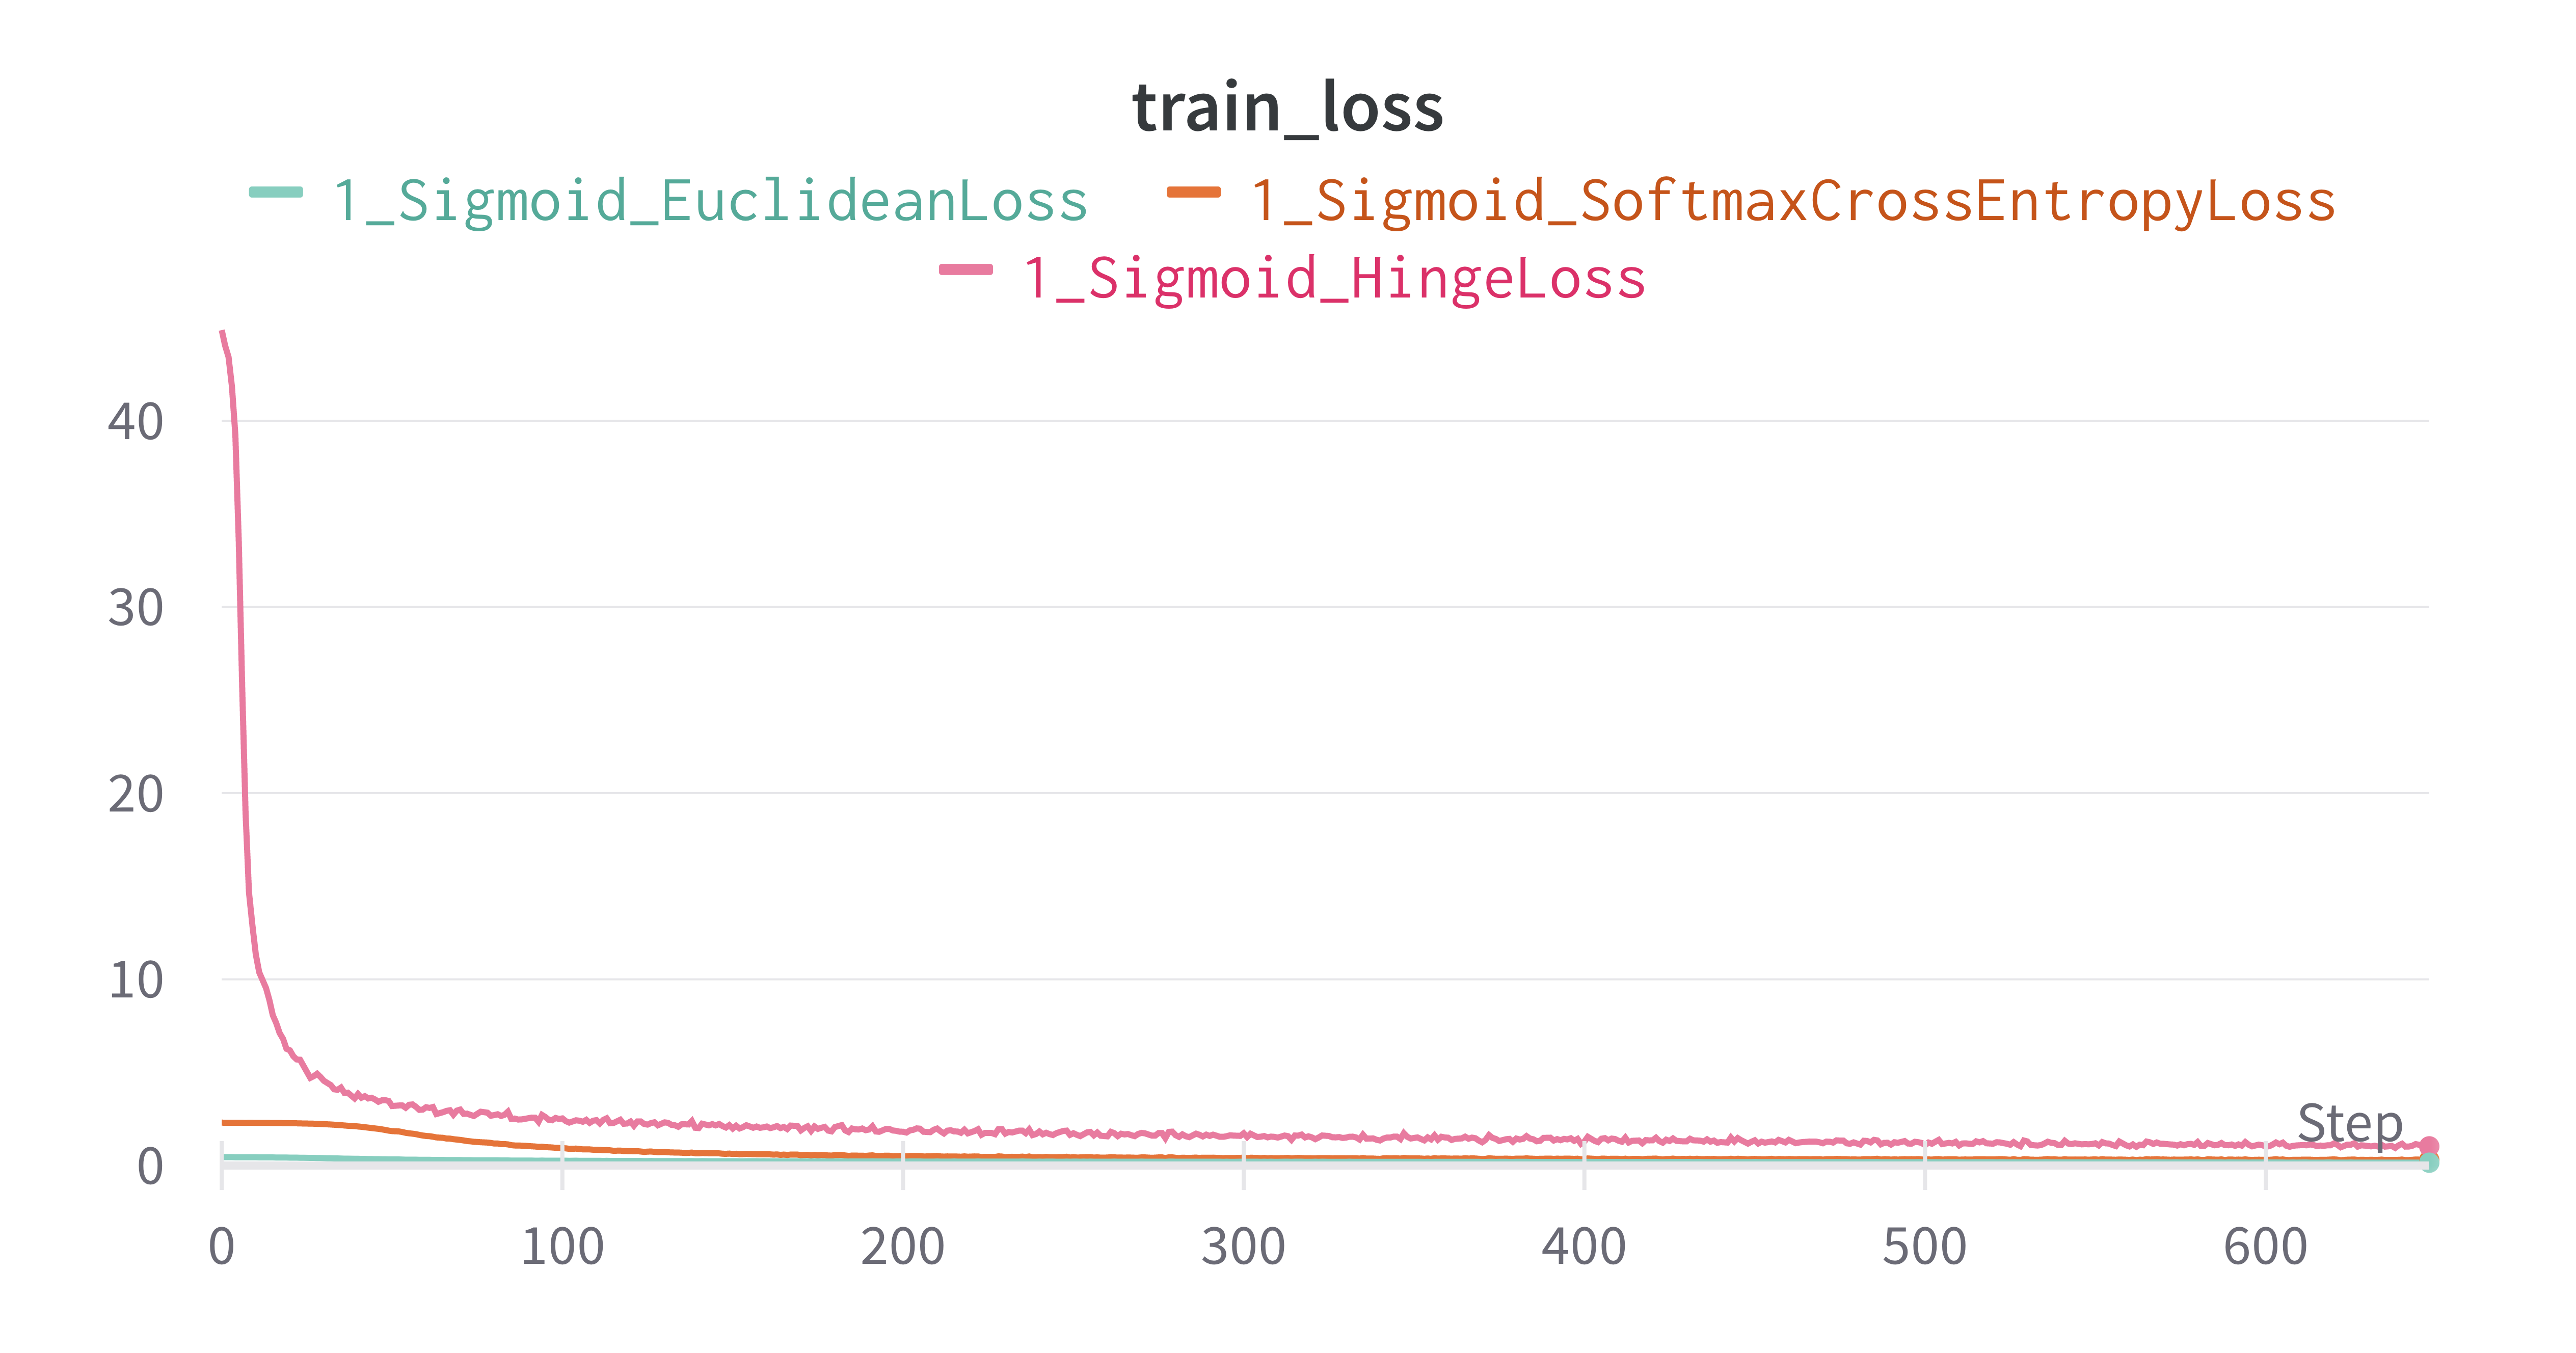
\includegraphics[width=1\textwidth]{../pics/单层损失函数train_loss.png}
		\caption{单隐藏层遍历损失函数对比 train loss}
	\end{subfigure}
	\begin{subfigure}{0.475\textwidth}
		\centering
		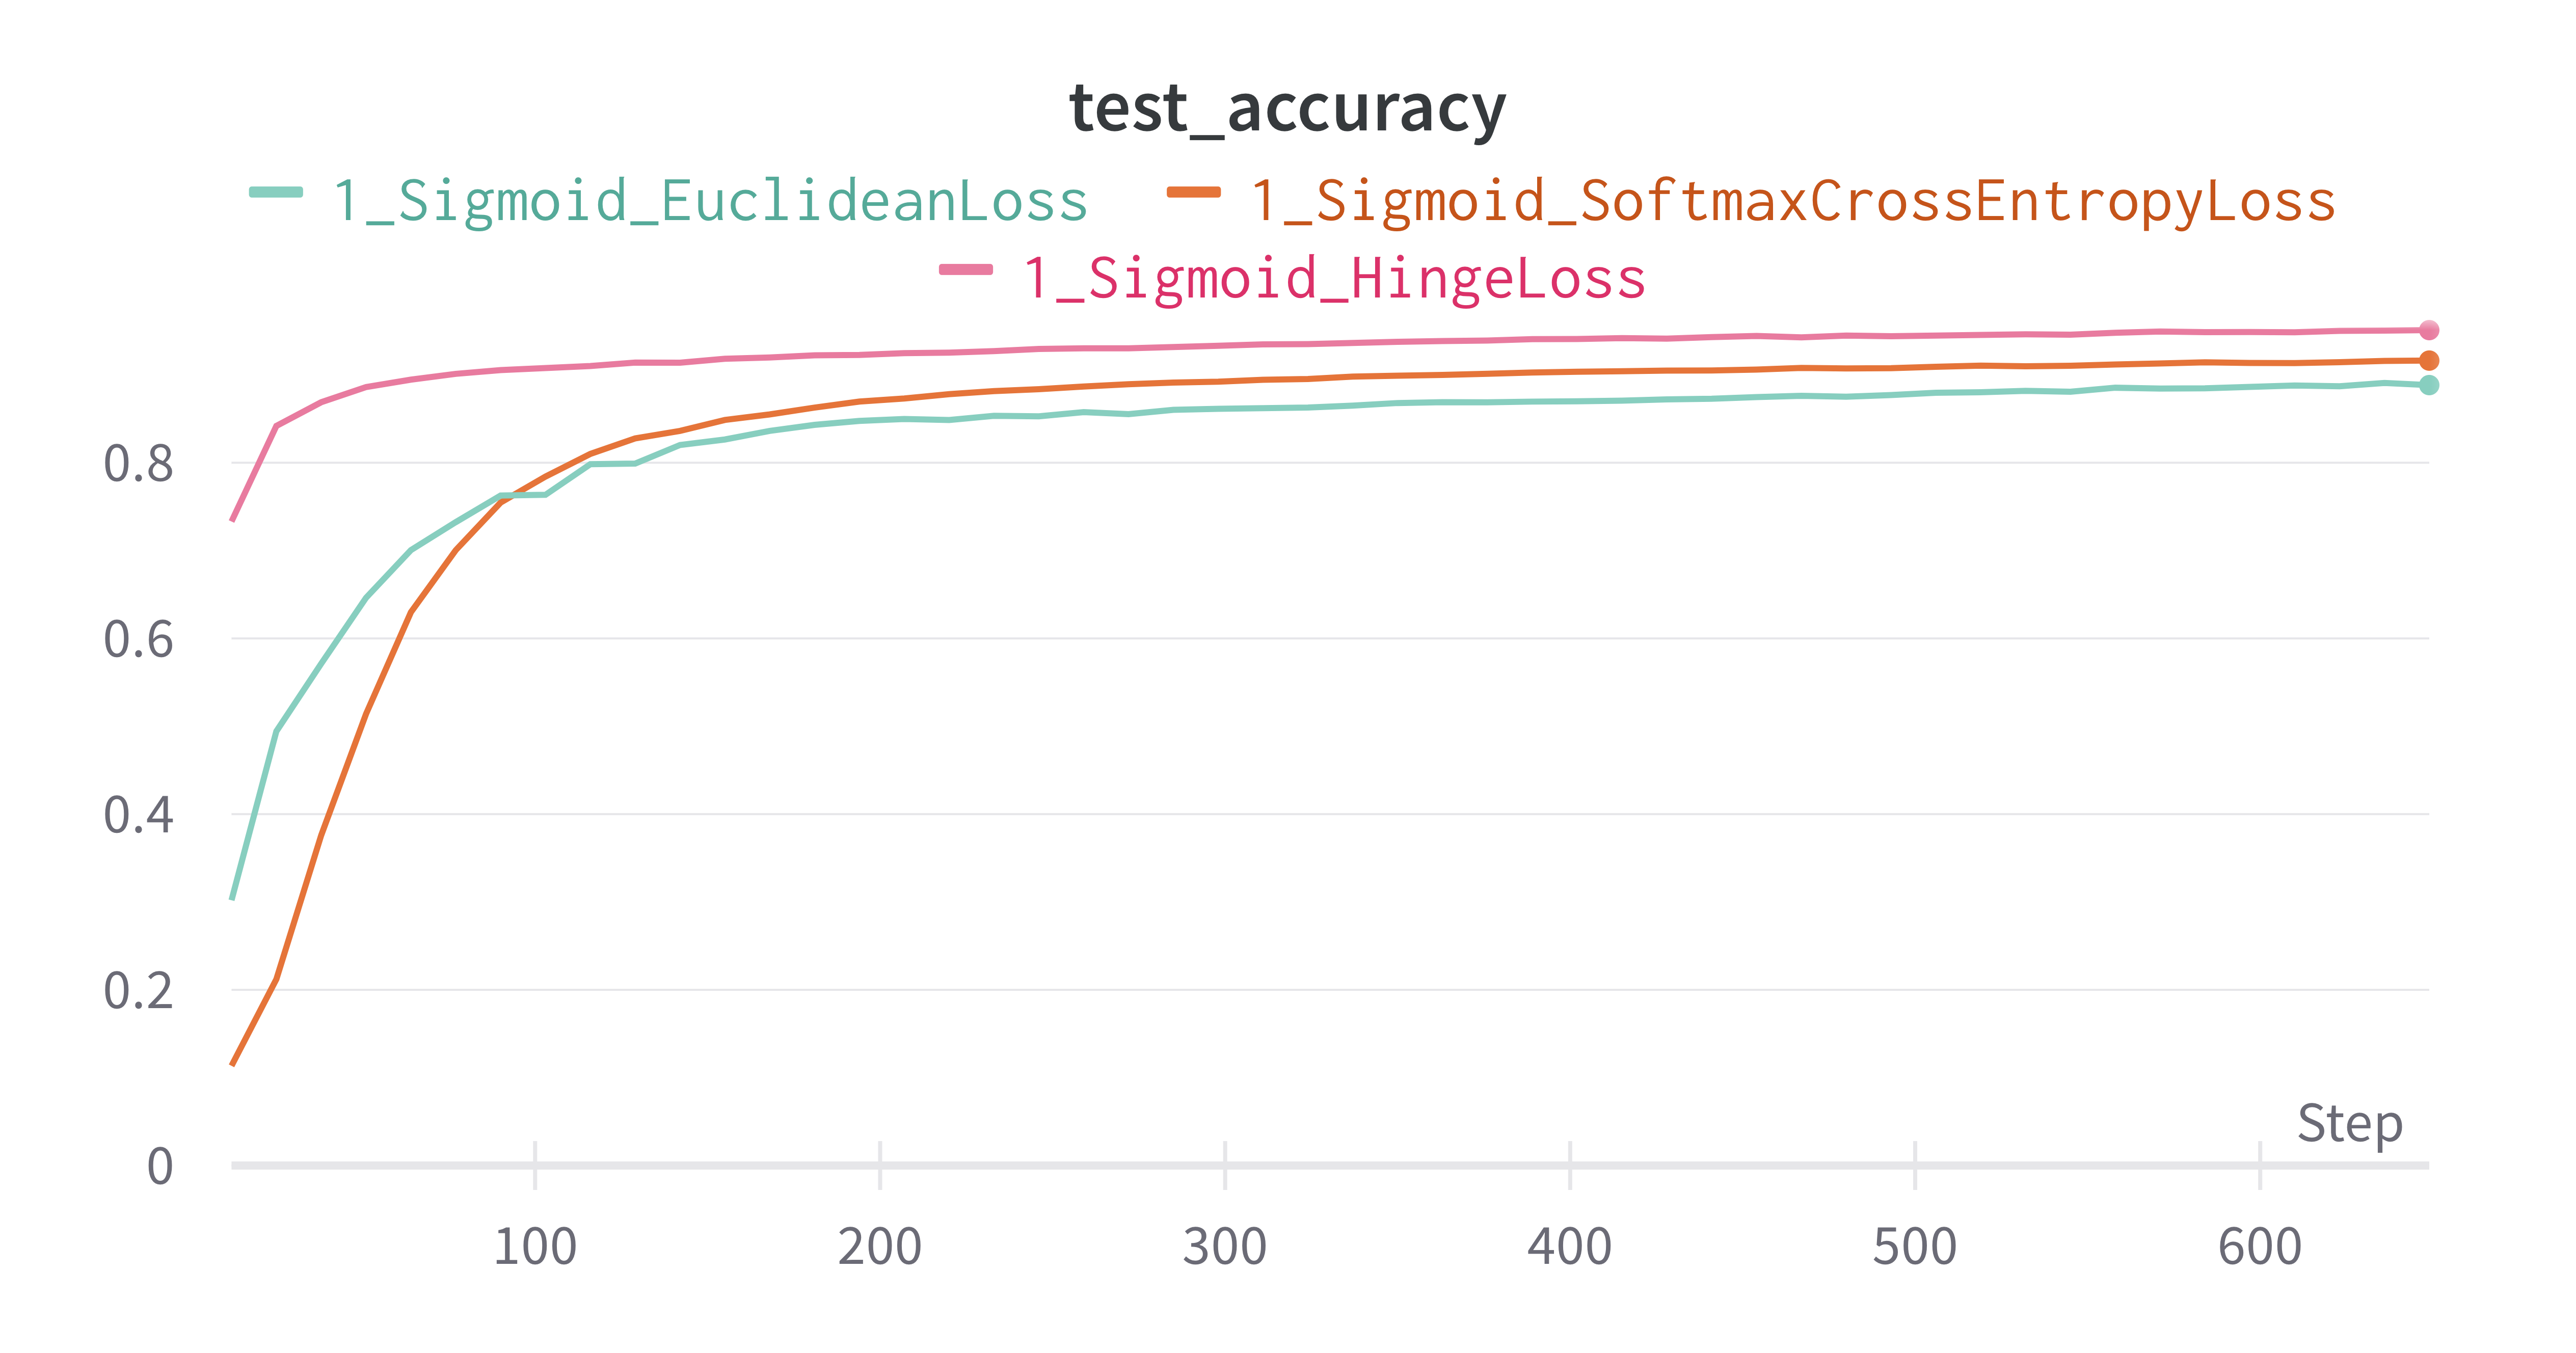
\includegraphics[width=1\textwidth]{../pics/单层损失函数test_acc.png}
		\caption{单隐藏层遍历损失函数对比 test accuracy}
	\end{subfigure}
	\begin{subfigure}{0.475\textwidth}
		\centering
		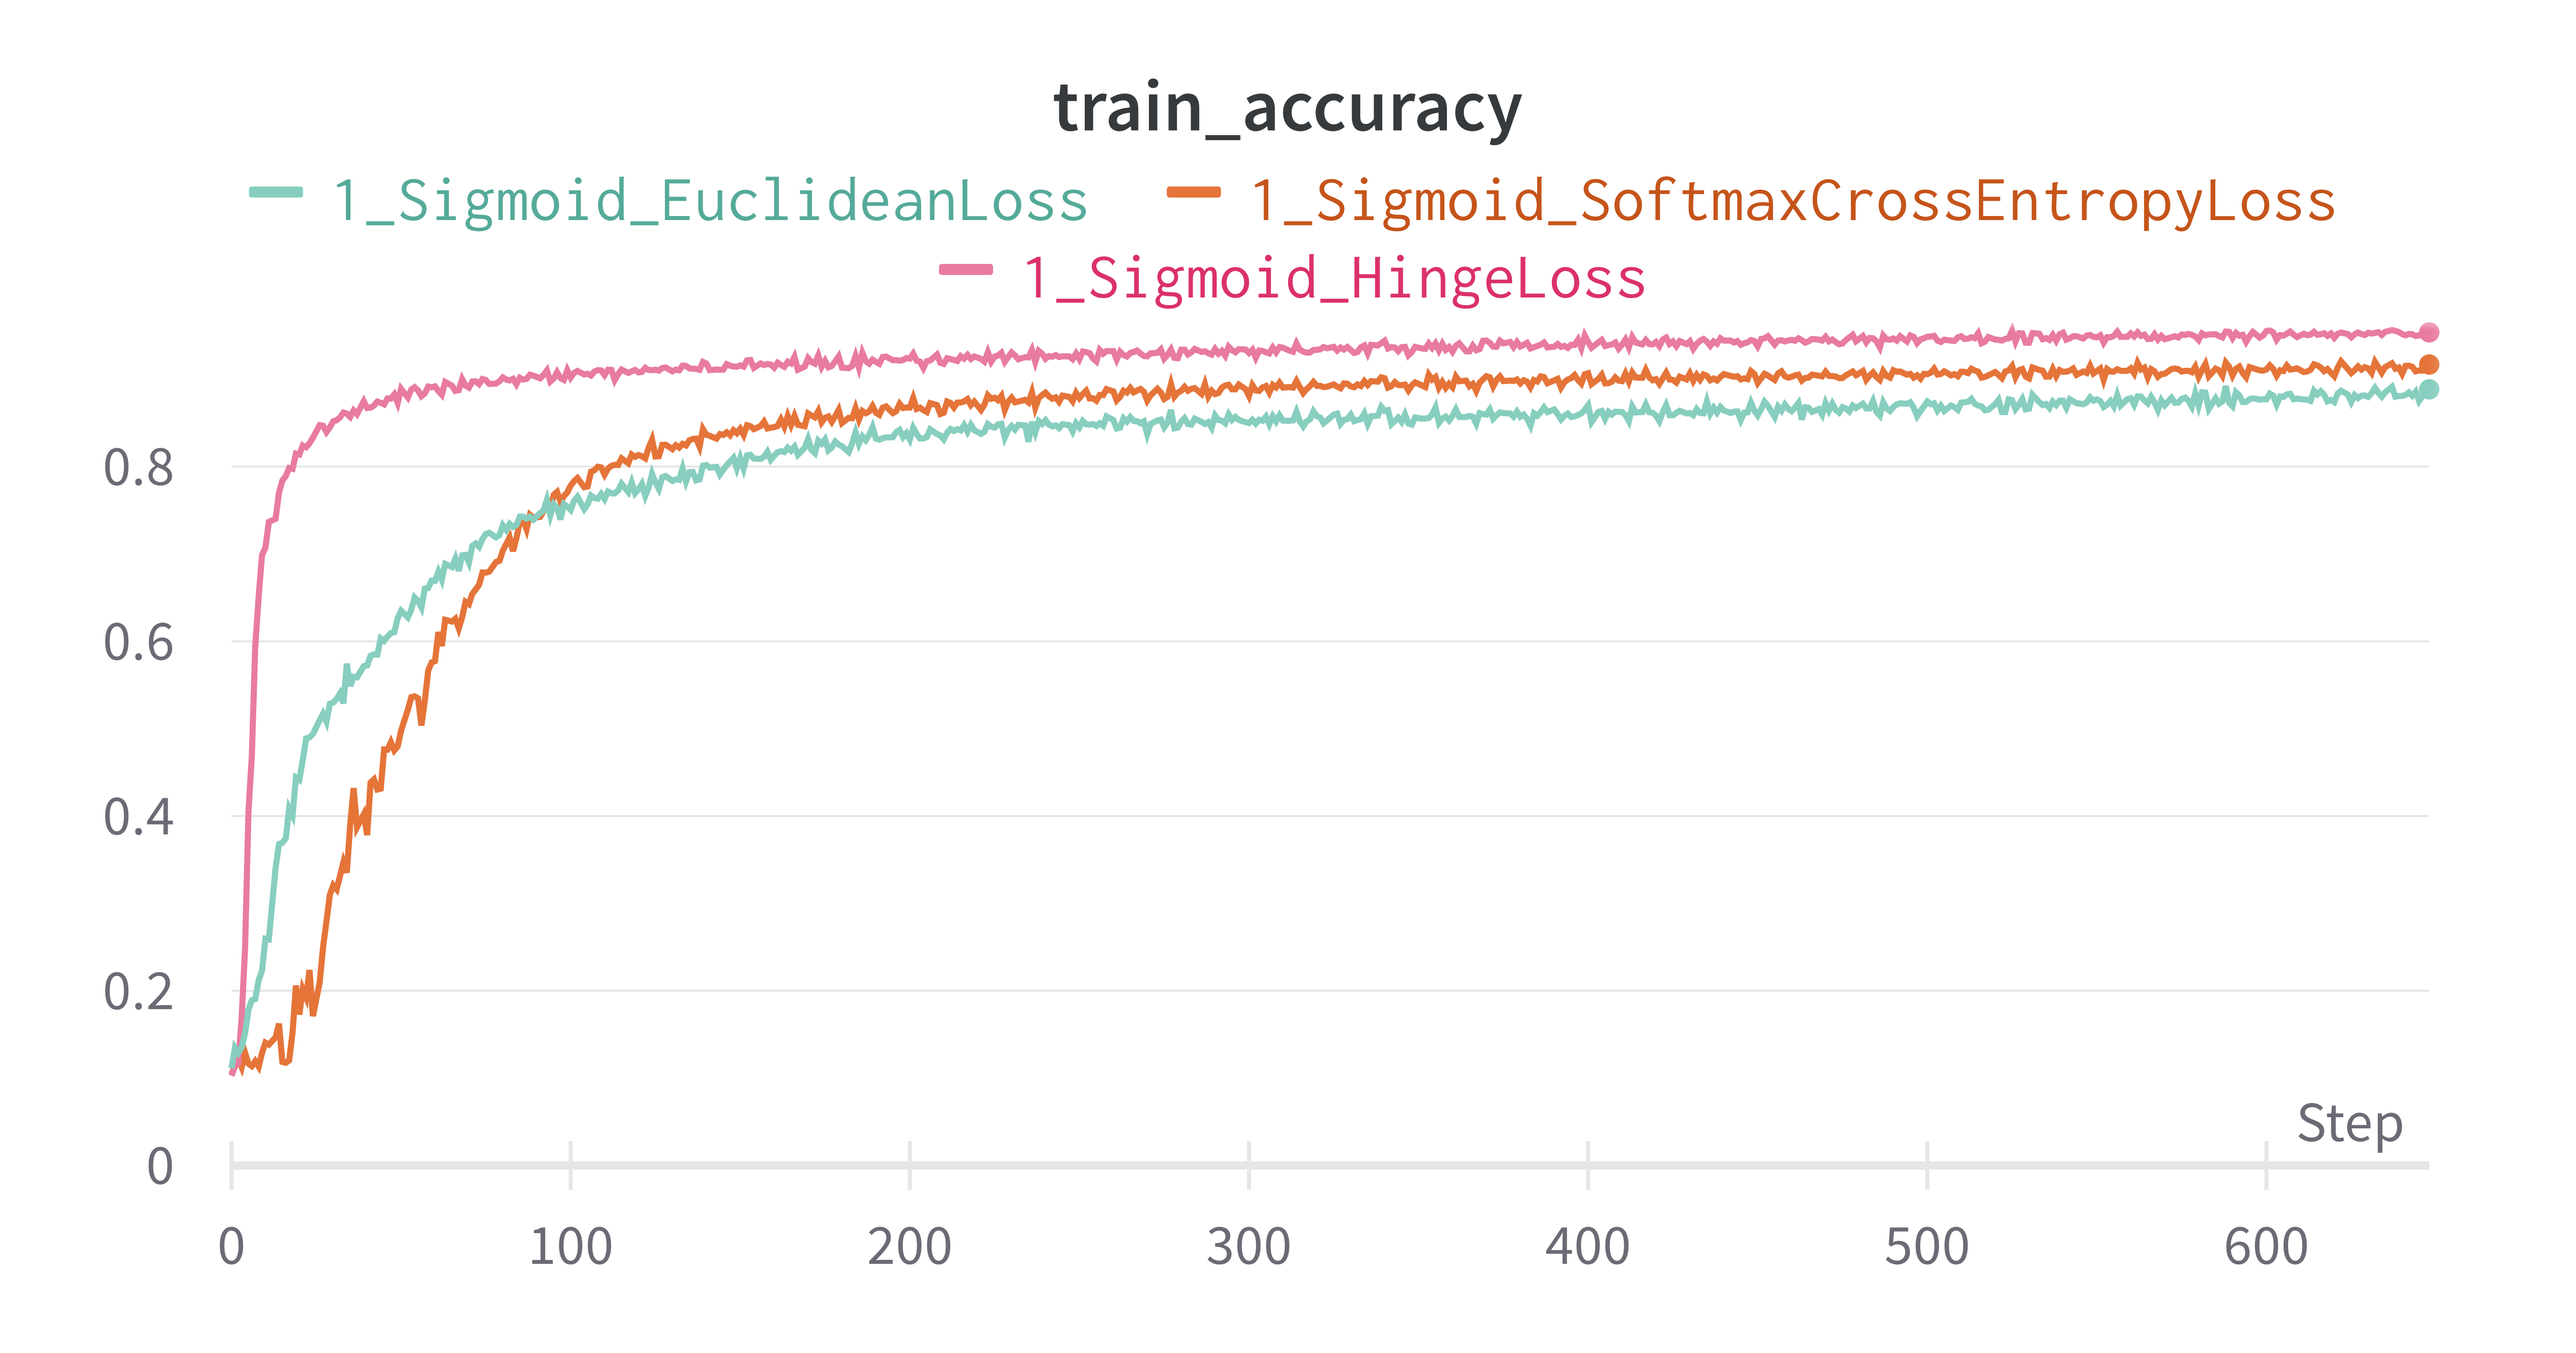
\includegraphics[width=1\textwidth]{../pics/单层损失函数train_acc.png}
		\caption{单隐藏层遍历损失函数对比 train accuracy}
		\label{fig:4d}
	\end{subfigure}
	\caption{单隐藏层遍历损失函数}
	\label{fig:4}
\end{figure}

比较 Hinge、SoftmaxCrossEntropy 和 Euclidean 的函数形式可见,Hinge 损失函数的计算形式最为复杂,效果出人意料更好。然而之前接触过的分类任务更多使用 SoftmaxCrossEntropy。没有选择使用 Hinge 的原因可能是 Hinge 还还存在超参数 Margin 的缘故;对于 Margin 参数的 tune 也能作为实验目标。\\
具体对比三个损失函数,做分析如下:

\begin{enumerate}
 	\item Softmax 的图像近似与经过平滑处理后的 Hinge,故而能够推断二者的训练效果相当。
 	\item Euclidean 的结果相比 Softmax 较差,这可以从训练目标角度进行理解。Euclidean 的训练目标是希望线性层输出的结果尽可能接近真实值,也即在一个 $\Re^n$ 空间上的输出结果尽可能接近一个 one-hot 向量;而 Softmax
 	的目标是线性层输出的结果映射到概率分布空间上尽可能接近真实值,也即在一个 $\Re^n$ 空间上的输出结果映射到一个概率分布空间后尽可能接近一个 one-hot 向量,考虑到概率分布空间本就是一个各维度之和为 1 的 $\Re^n$ 子空间,这与 one-hot 分布的空间是完全相同的。
	故而 Softmax 损失函数的训练目标更为优化,能够理解更好的训练效果。举例而言,如果线性层最后输出向量 $(0, 0, 0, 100)^T$,而期望的 one-hot 向量是 $(0, 0, 0, 1)^T$。对于 Euclidean 而言,这个输出结果非常糟糕,
	损失值大,模型会惩罚当前的参数,使得输出结果的最后一项降低直至接近 $(0, 0, 0, 1)^T$;然而,对于 Softmax 而言,这个输出结果非常好,经过 Softmax 后,线性层的输出向量高度接近 $(0, 0, 0, 1)^T$,这一损失值很小,
	模型会倾向于奖励当前的参数。
	\item Euclidean 虽然训练目标和 one-hot 分类并不相近,最终会遏制模型的表达能力,然而 Euclidean 在训练初始时的损失值较大,收敛速率相对更高,这能够在图 \ref{fig:4d} 从 Euclidean 和 Softmax 的训练集正确率曲线梯度的对比中可以看出。
\end{enumerate}


\subsubsection{不同激活函数对比}

在单隐藏层的前提下,固定损失函数为 Euclidean,遍历三种激活函数,结果如图 \ref{fig:5} 所示。

\begin{figure}[htbp]
	\centering
	\begin{subfigure}{0.475\textwidth}
		\centering
		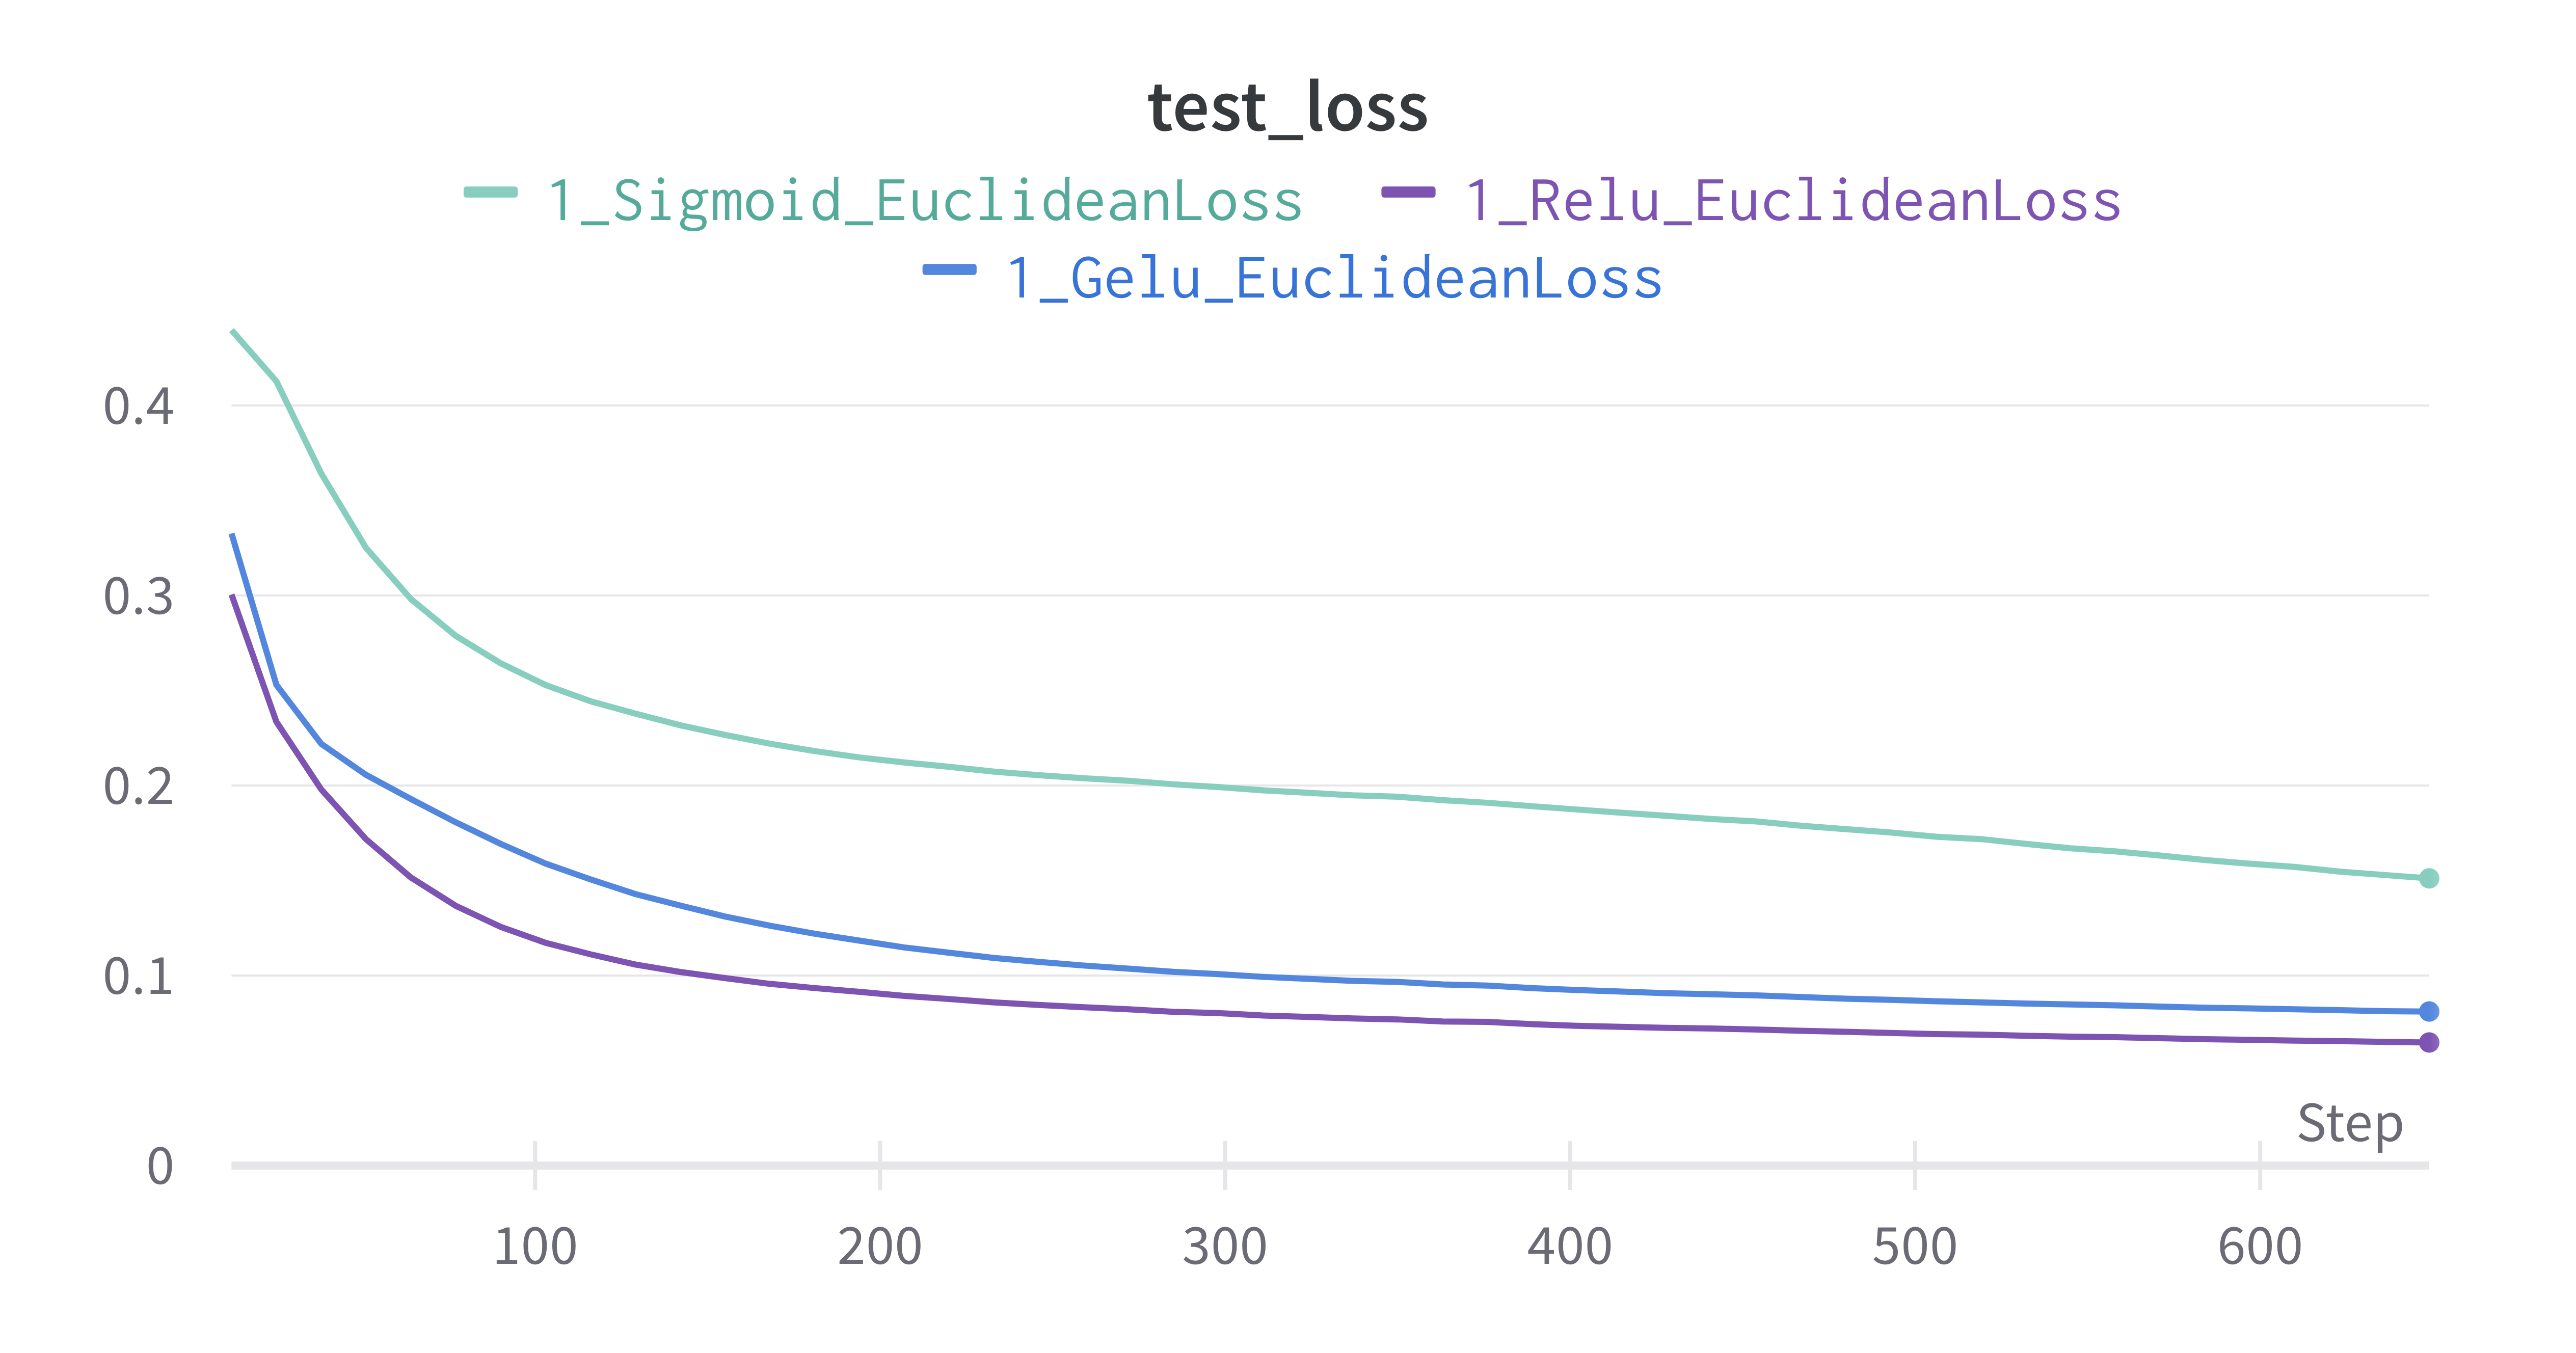
\includegraphics[width=1\textwidth]{../pics/单层激活函数test_loss.png}
		\caption{单隐藏层遍历激活函数对比 test loss}
	\end{subfigure}
	\begin{subfigure}{0.475\textwidth}
		\centering
		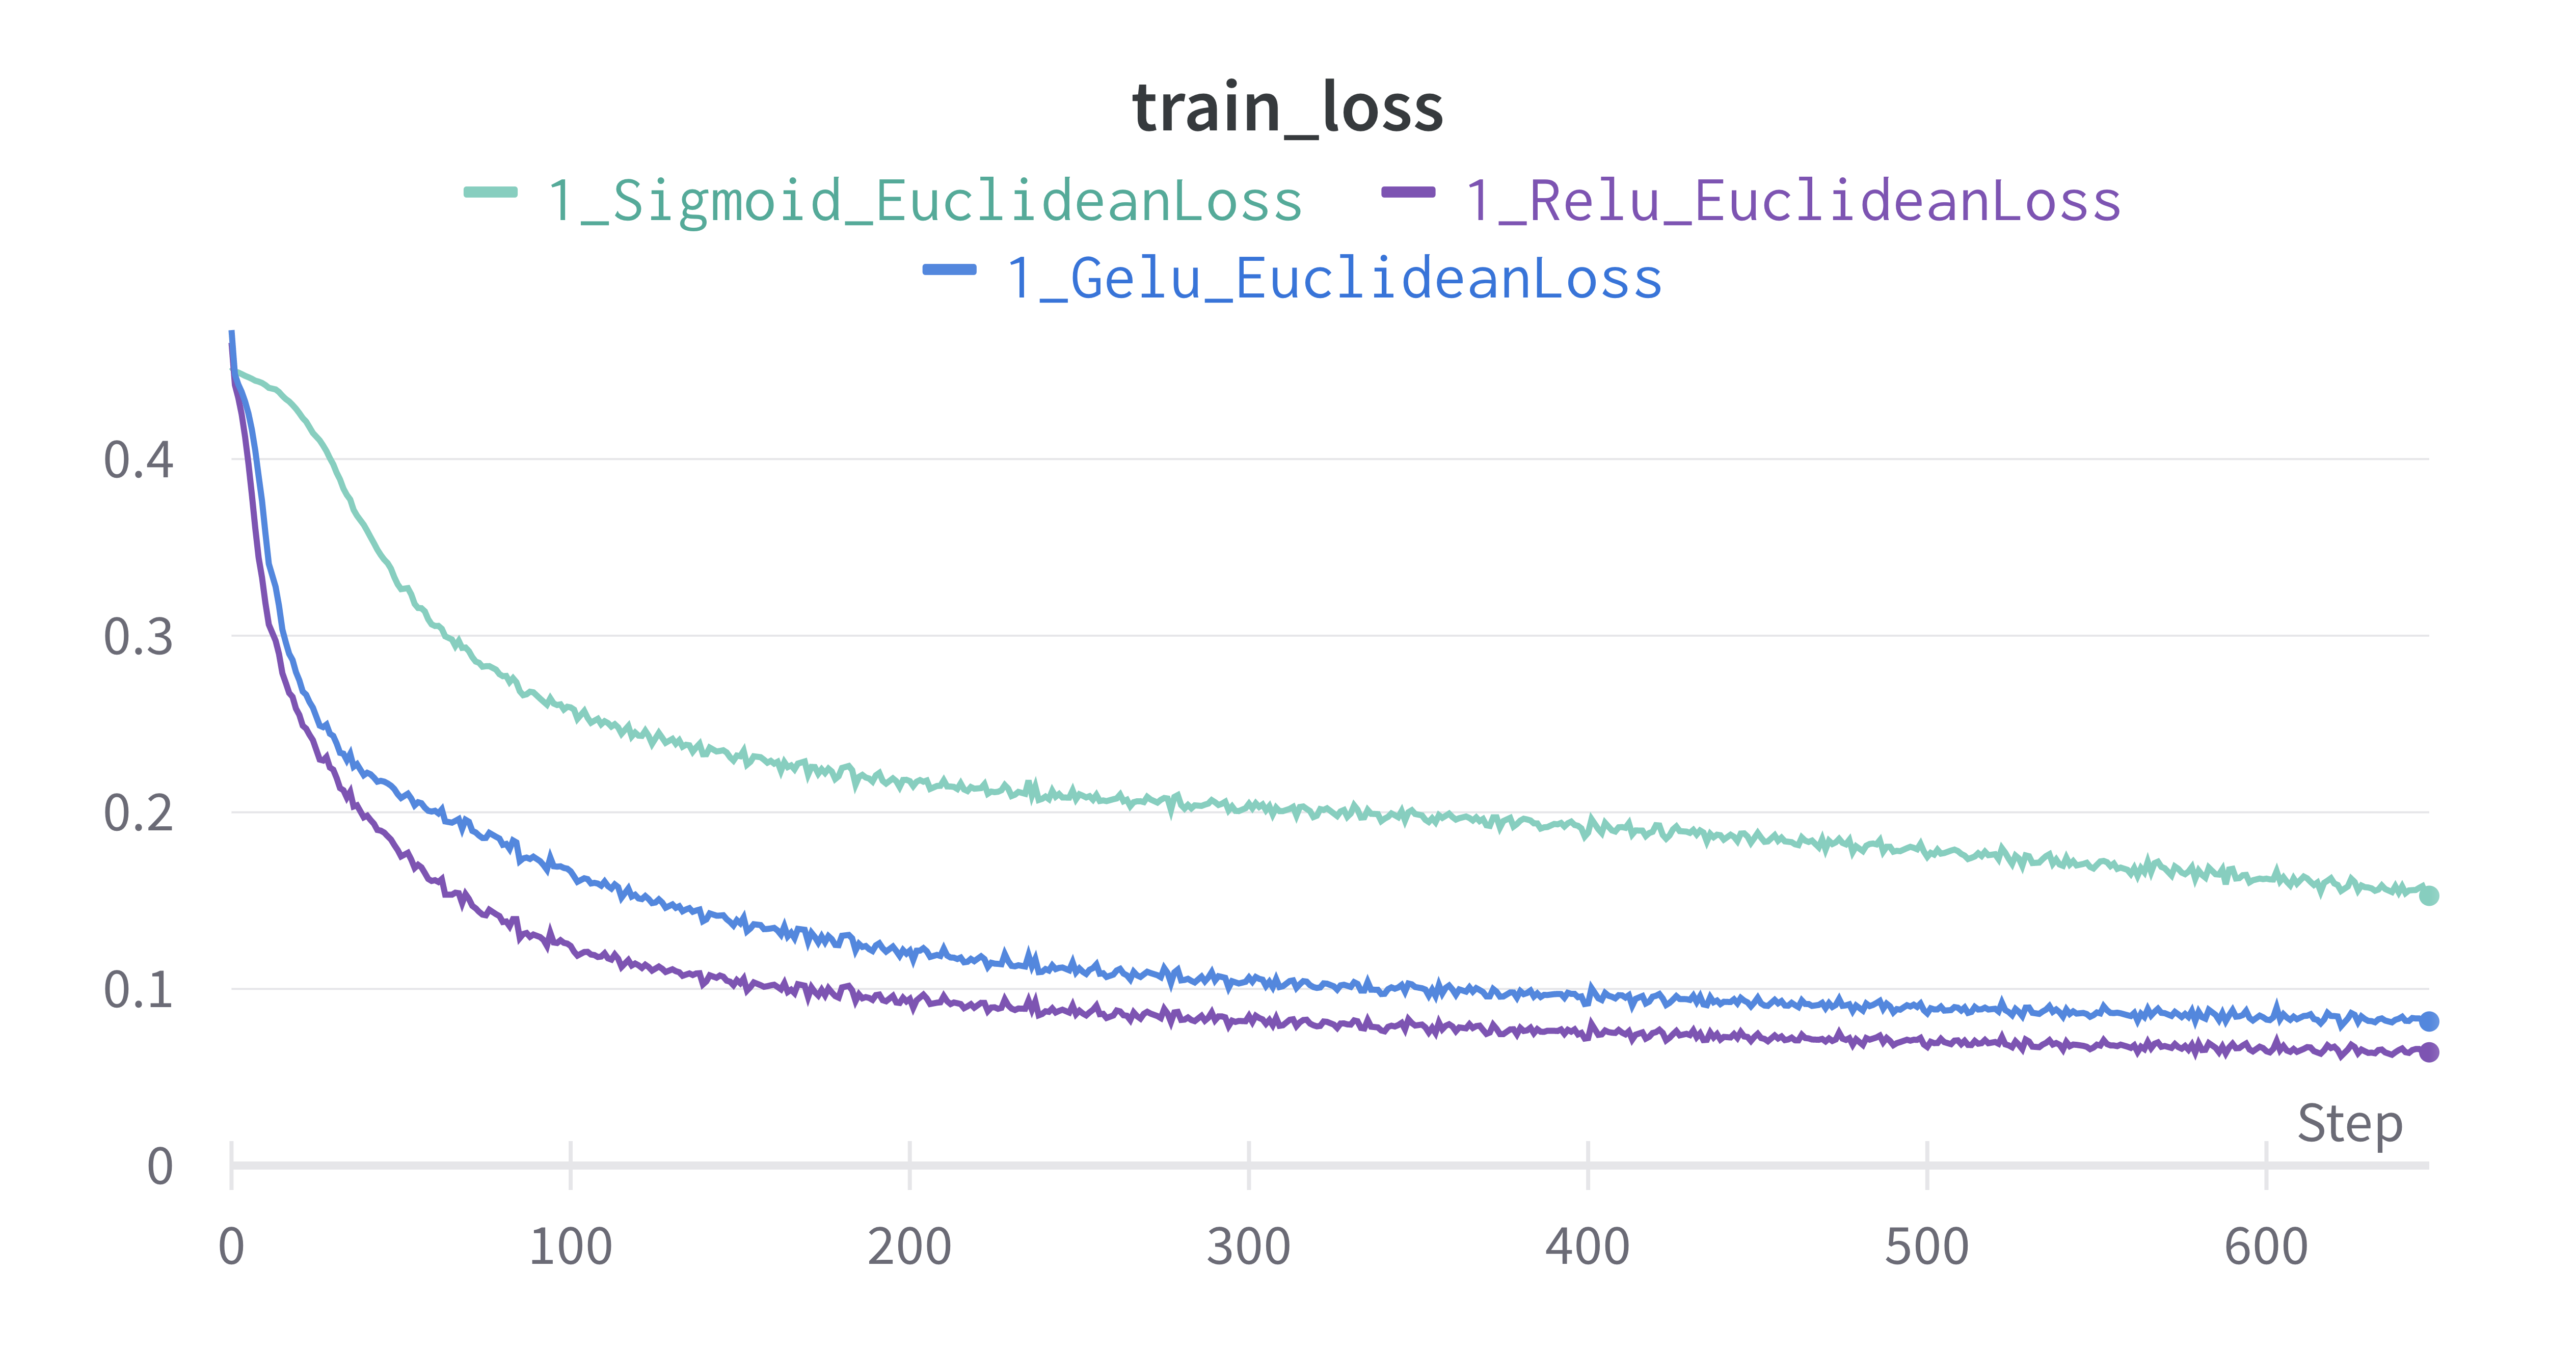
\includegraphics[width=1\textwidth]{../pics/单层激活函数train_loss.png}
		\caption{单隐藏层遍历激活函数对比 test loss}
	\end{subfigure}
	\begin{subfigure}{0.475\textwidth}
		\centering
		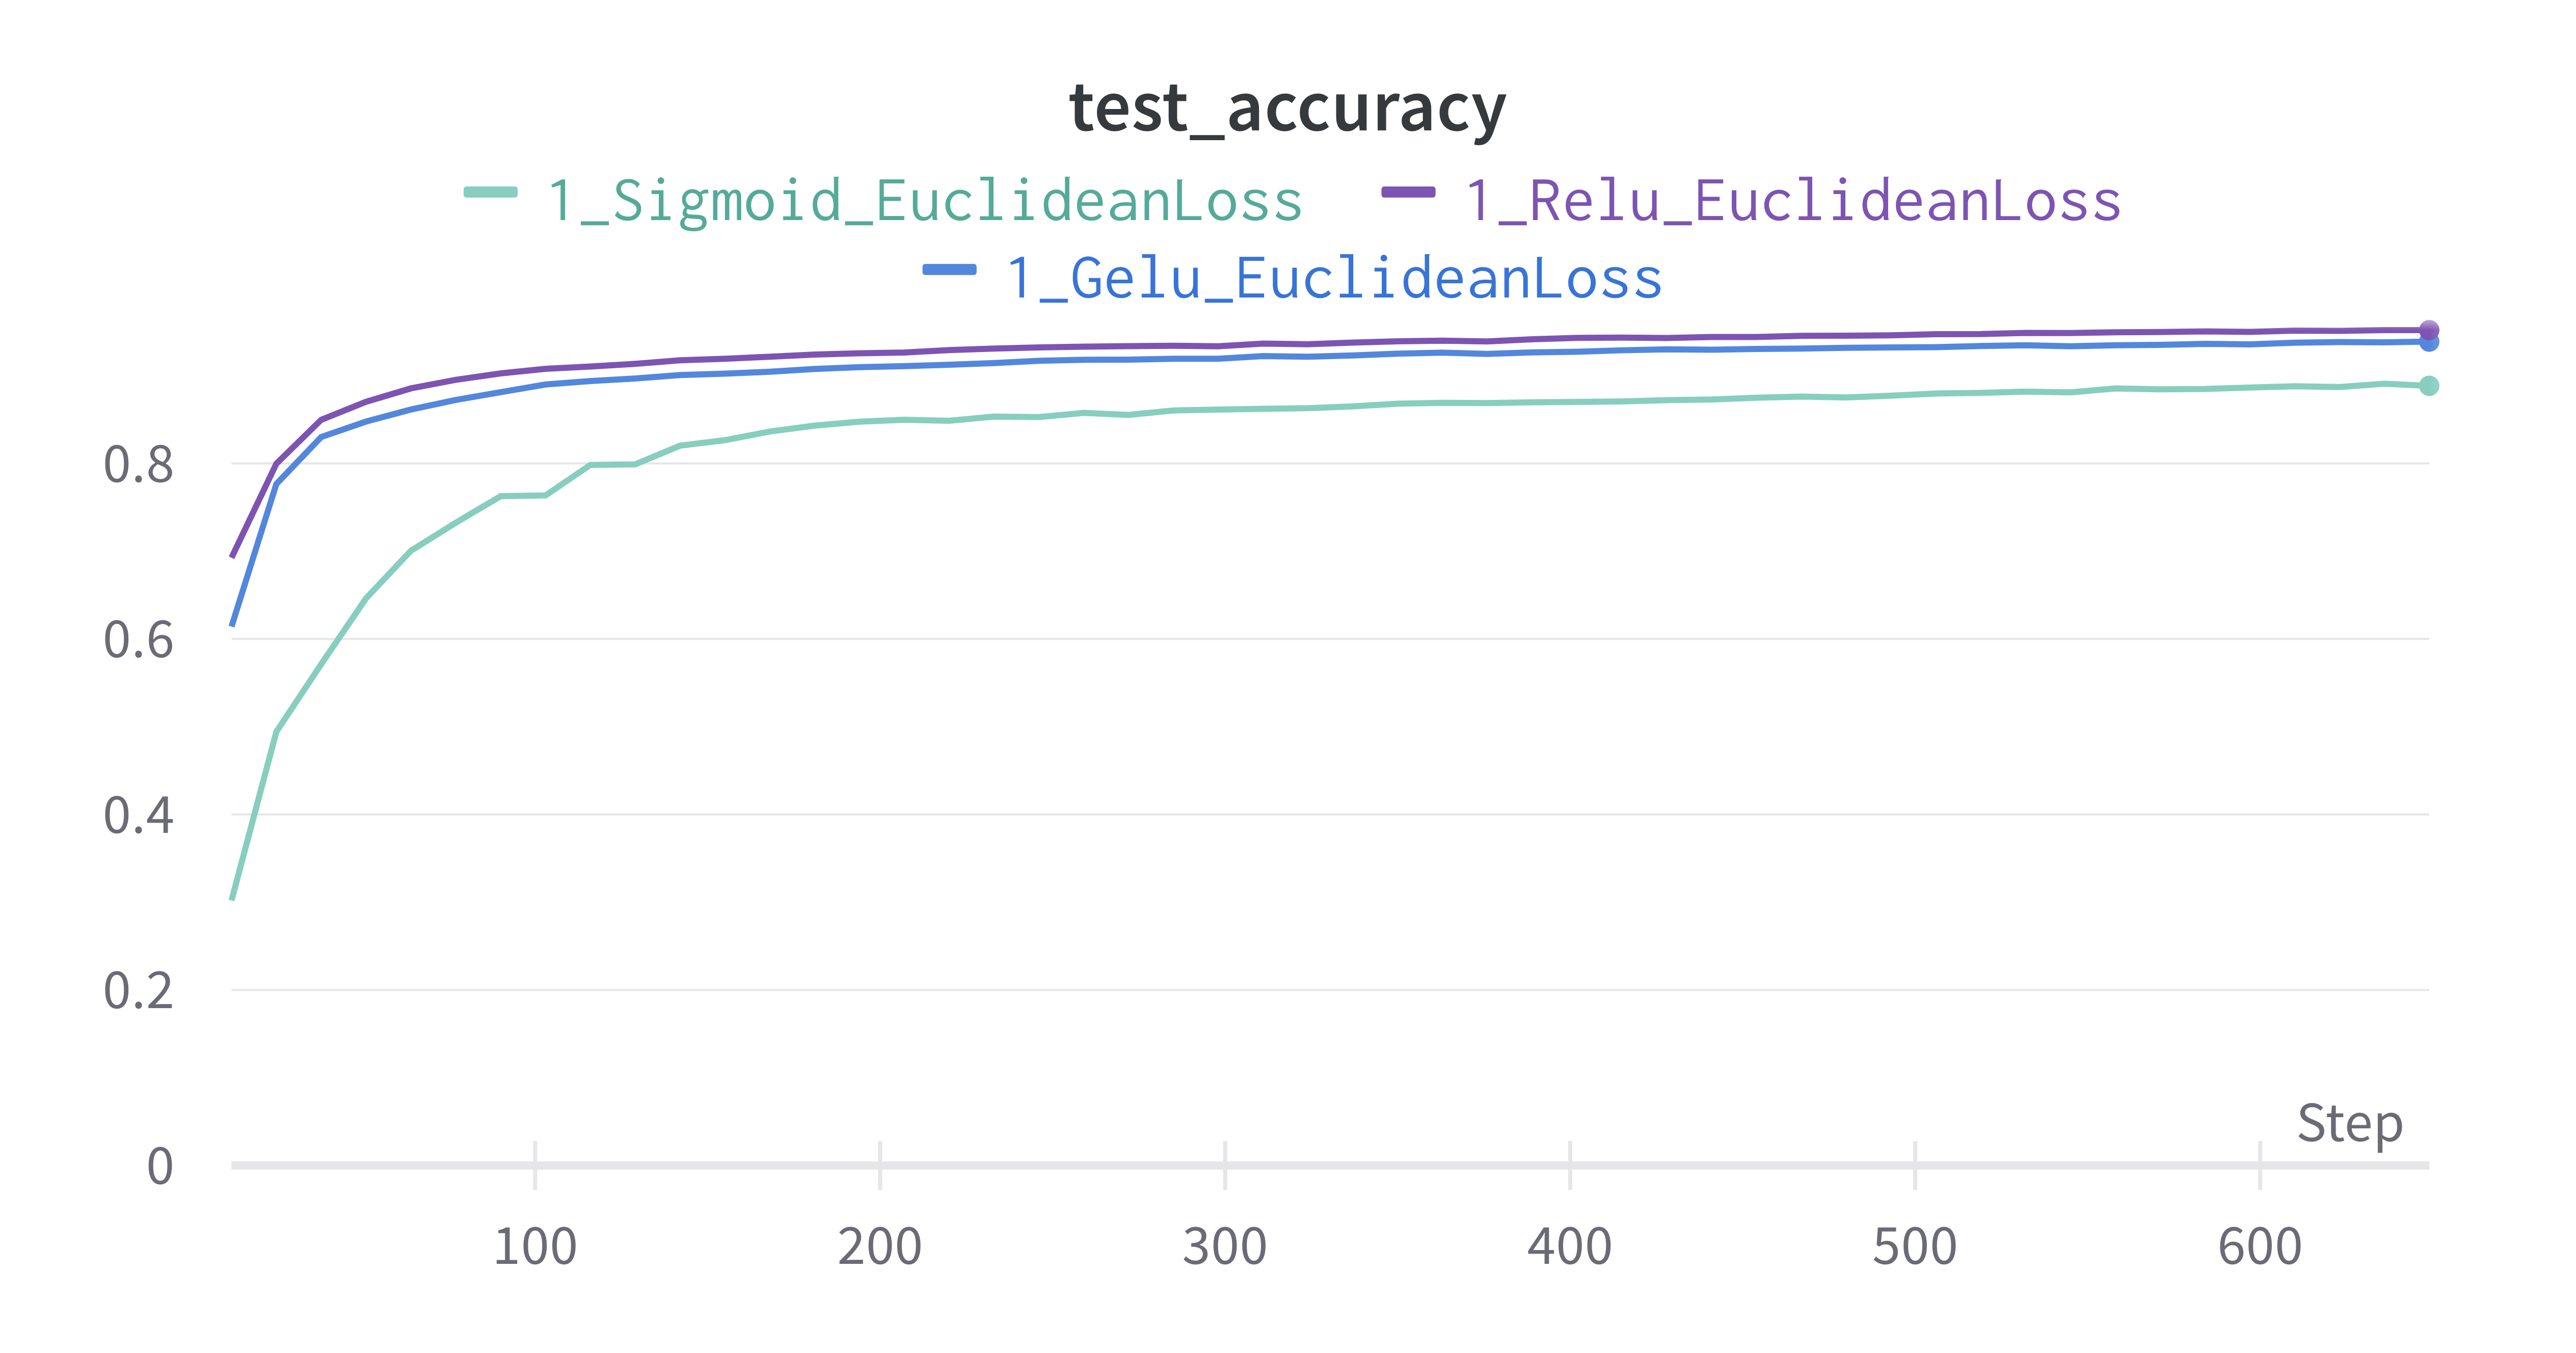
\includegraphics[width=1\textwidth]{../pics/单层激活函数test_acc.png}
		\caption{单隐藏层遍历激活函数对比 test loss}
	\end{subfigure}
	\begin{subfigure}{0.475\textwidth}
		\centering
		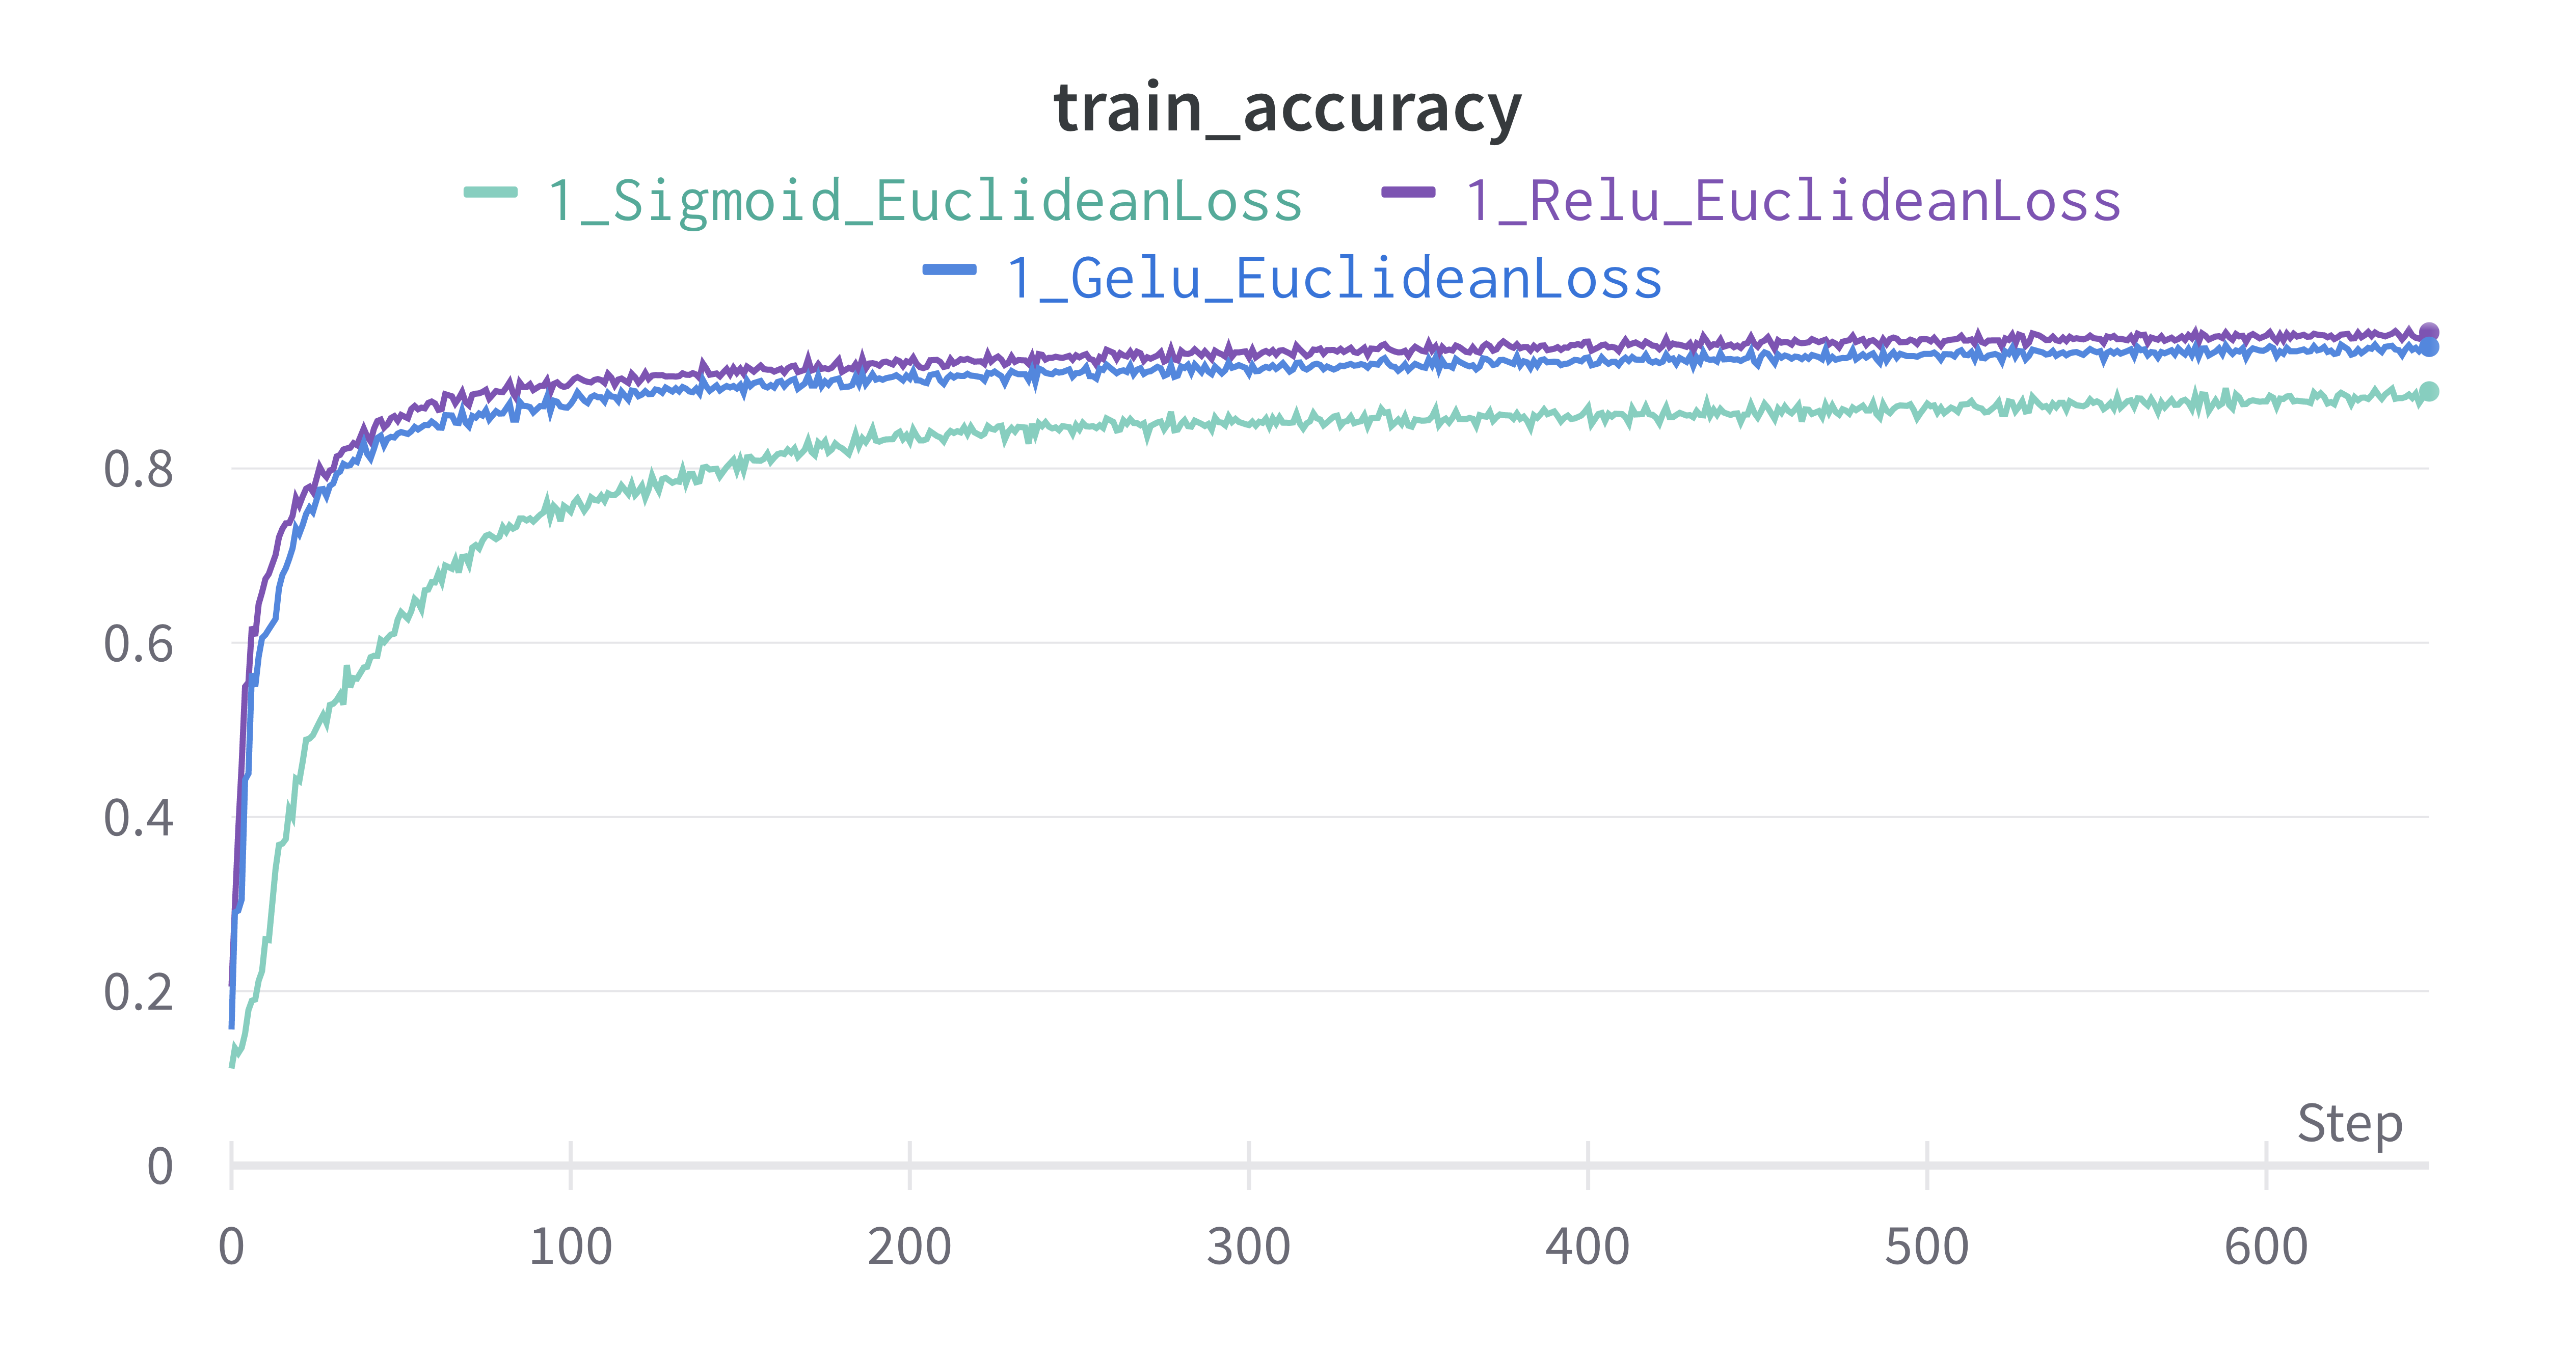
\includegraphics[width=1\textwidth]{../pics/单层激活函数train_acc.png}
		\caption{单隐藏层遍历激活函数对比 test loss}
	\end{subfigure}
	\caption{单隐藏层遍历激活函数}
	\label{fig:5}
\end{figure}

分析结果可以发现,(1)就准确率而言,ReLU 结果略微高于 GeLU,而 Sigmoid 的表现与二者有一定差距;(2)就损失值而言,ReLU 损失值略微低于 GeLU,而 Sigmoid 损失值显著大于前两者,且损失值衰减速率基本与准确率的上升速率符合;(3)就收敛速度而言,ReLU 与 Gelu 收敛速度相当,而 Sigmoid 收敛最慢,且收敛值最低;(4)就训练时间而言,Sigmoid 耗时为 29s,Relu 为 22s,Gelu 为 47s,考虑到 Relu 最为简单的函数形式,具有最快的训练速度符合预期。而 Gelu 的实现方式基于微分的极限定义,计算复杂度最高,也符合预期。

对比图 \ref{fig:5},考虑到三者的函数定义。
\begin{itemize}
    \item $Gelu(x)=x \times P(X<=x)=x \times \phi(x), x \sim N(0,1) \approx  0.5 \times x\left(1+\tanh \left[\sqrt{\frac{2}{\pi}}\left(x+0.044715 x^3\right)\right]\right)$
    \item $Relu(x)=x^{+}=\max (0, x)$
    \item $Sigmoid(x)=\frac{1}{1+e^{-x}}=\frac{e^x}{e^x+1}=1-Sigmoid(-x)$
\end{itemize}

Sigmoid 和 GeLU 光滑且连续可微的函数;而 GeLU 被誉为平滑的 ReLU,二者图像和导数值相近,在损失值为正时,具有相对稳定的导数。然而,Sigmoid 的效果一贯较差是深度学习领域研究者多年得出的一贯结论。具体而言,Sigmoid 在损失值较大时,实际上倒数值偏小,梯度消失非常严重。而我们观察到对 Euclidean 损失而言,初始的损失值就是偏大的,导致 Sigmoid 一直处于倒数值偏小的区间,严重限制了收敛效率与最终的收敛效果。

\subsubsection{过拟合问题}

实际上在本次实验中并未出现明显的过拟合现象,基本上实验结果保证了 loss 和 accuracy 负相关。然而,这一现象实际上并不绝对,在复杂模型处理复杂任务的情况下,往往会出现严重的过拟合。此外,即便是将 weight decay 设置为 0,也没有出现过拟合,实际上预示了 weight decay 参数可能对实验效果有着负面影响,而这在 \ref{paragraph:1} 一节得到了印证。

\subsection{双隐藏层实验}

增加双层隐藏层,隐藏层神经元数分别设置为 100 和 100,遍历不同损失函数和激活函数进行实验,得到的训练过程和训练结果分别如图 ~\ref{fig:6} 所示。相比同样单隐藏层训练结果,双隐藏层的网络在测试集、训练集上的表现并未比单隐藏层存在显著优势,甚至在许多模型设定下表现不如单隐藏层。出于常识,双隐藏层网络比单隐藏层网络拥有更多的参数,似乎该具有更强的学习能力。\\
然而,这个结论并不必然。一方面,小模型并不意味着更弱的表现能力,知识蒸馏领域的研究者便希望能够用更小的模型达到更好的效果;另一方面,在这次实验中,双层的参数复杂度上升,需要的训练资源和训练技巧相应更多,
然而实验过程并没有为模型添加 dropout 层与 batch norm 层,也没有参考 RNN 的实现而为双层模型使用 residual connection。另外,实验没有尝试调整 momentum 参数,而将其固定为 0.0,这等效于使用了最为原始的 SGD 优化器,进一步致使模型难以体现出增加隐藏层带来的表达力优势。最后,考虑到十分类任务本身已经足够简单,即便是最简单的单隐藏层 MLP 也有了几乎完全正确的结果,可见单层模型的表达能力已经足够强大;
双层模型并不能在模型表达力上有大幅突破,反而因为训练难度、模型复杂度和对训练技巧的更高需求丧失了潜在的优势。\\
综上所述,双隐藏层的结果不如单隐藏层,能够得到充分的理解。
\begin{figure}[htbp]
	\centering
	\begin{subfigure}{0.475\textwidth}
		\centering
		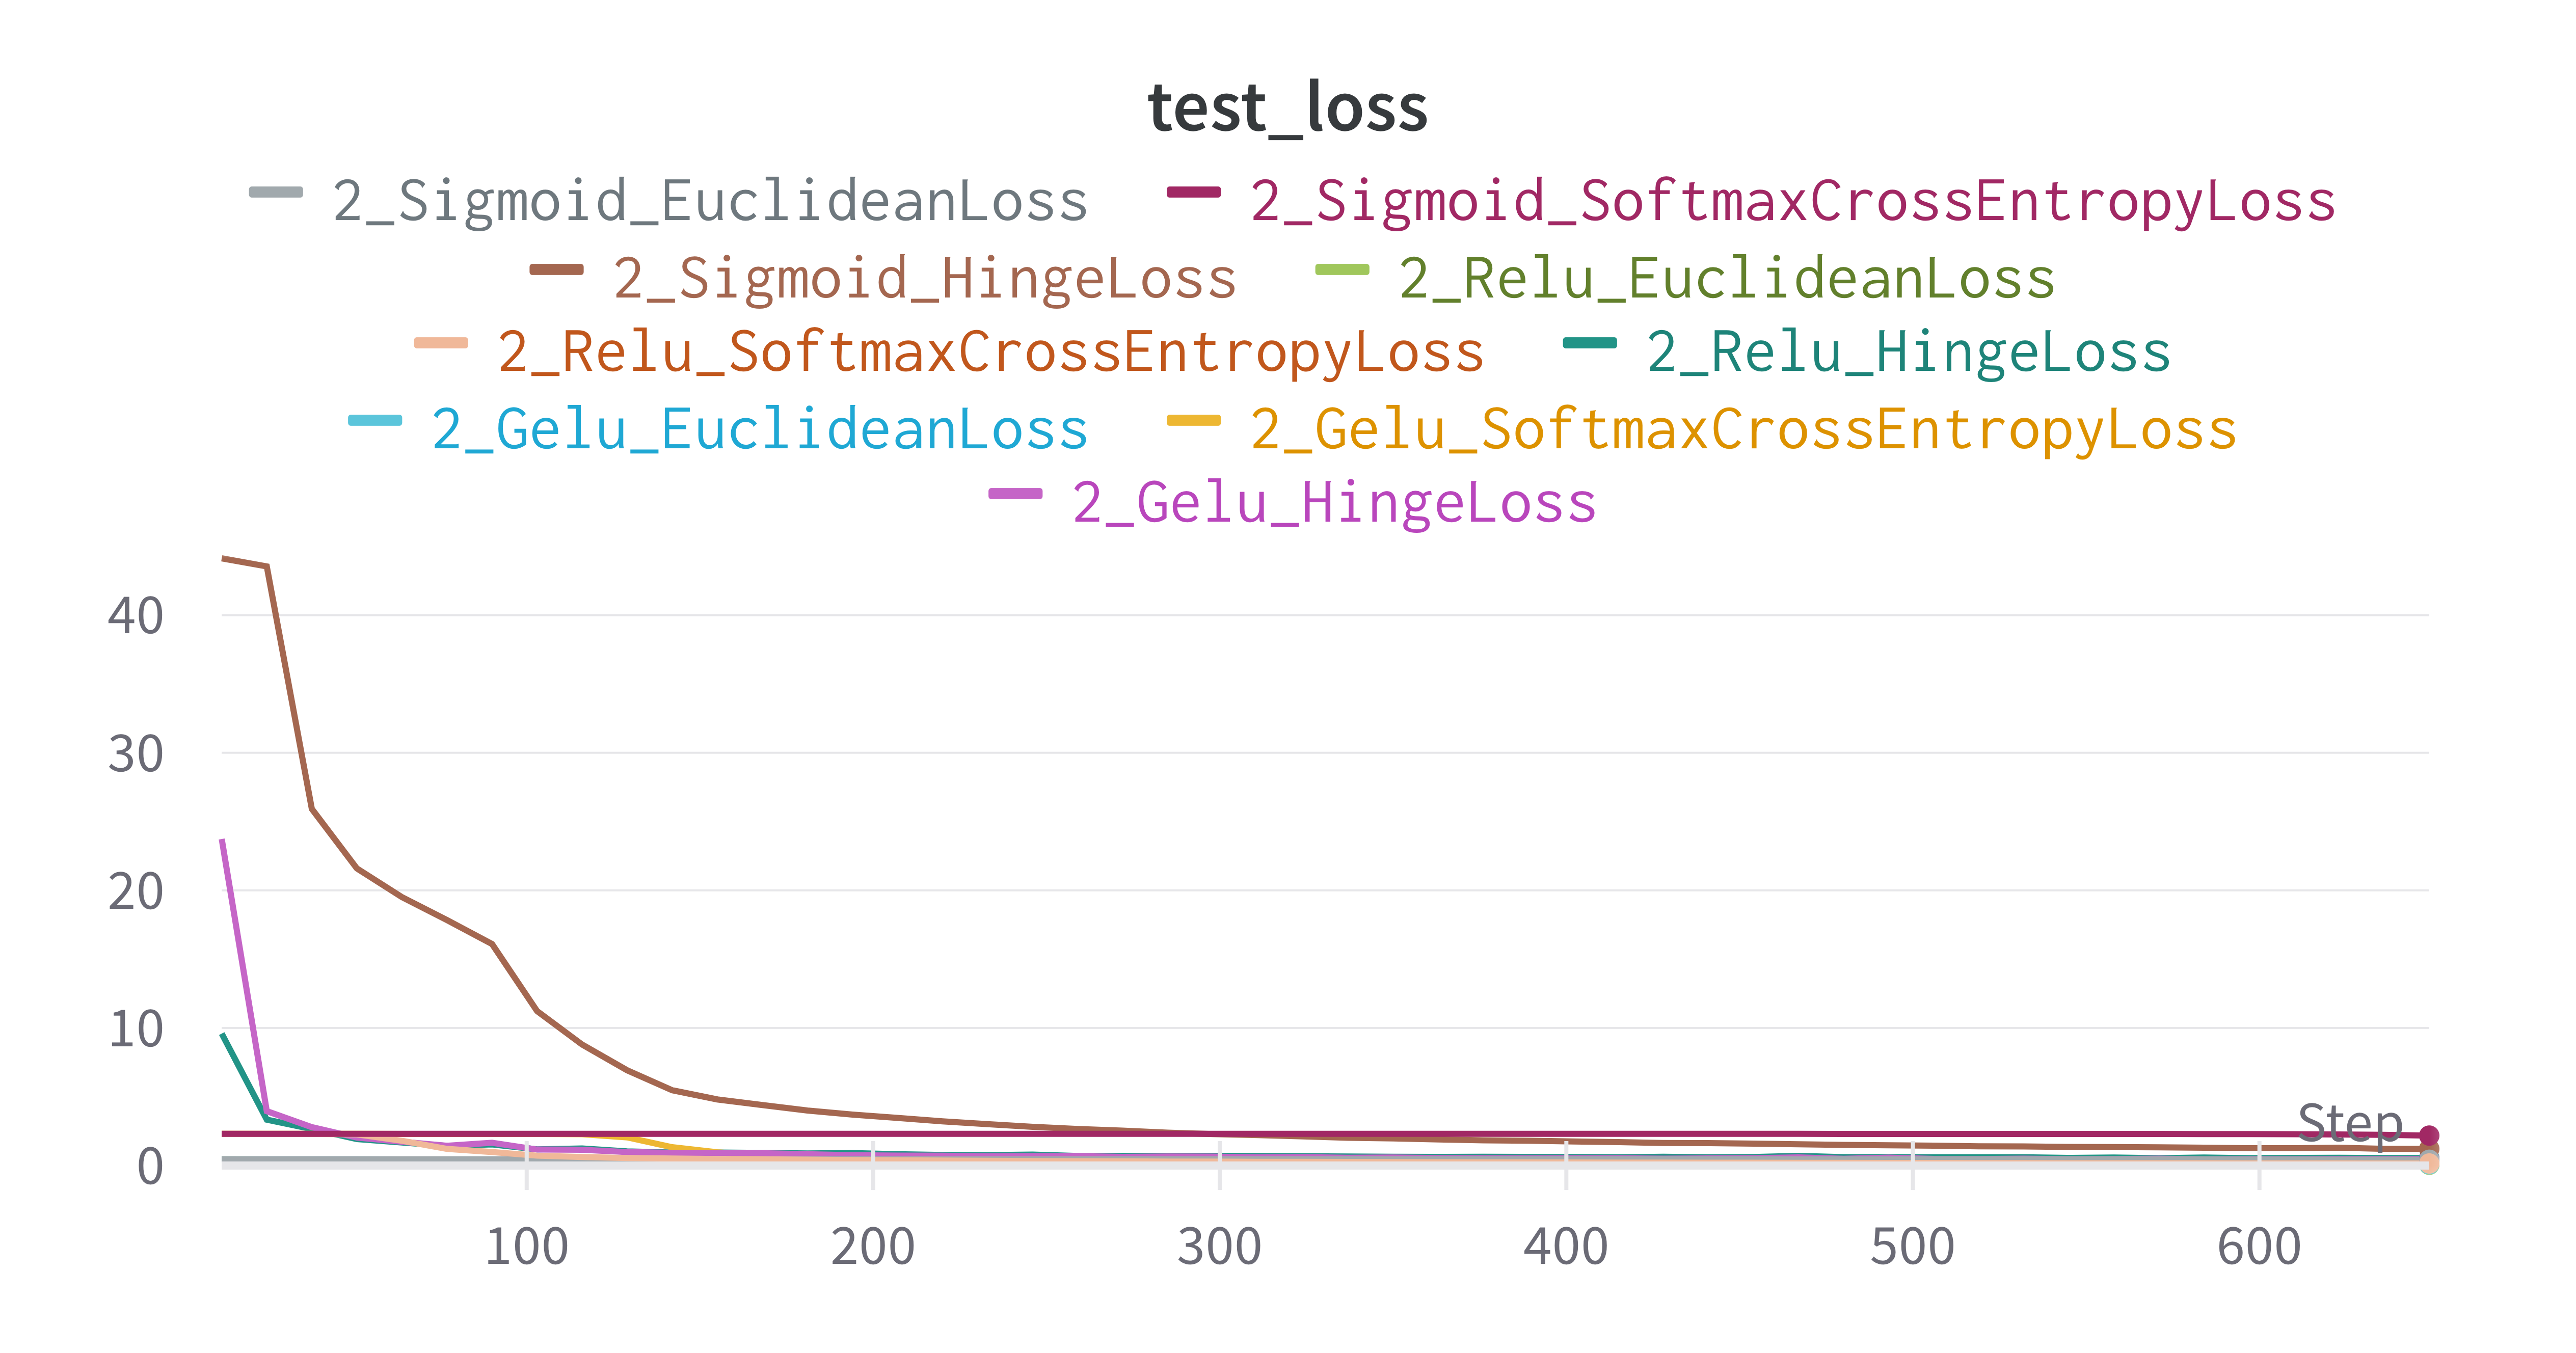
\includegraphics[width=1\textwidth]{../pics/双层实验-test_loss.png}
		\caption{双隐藏层 test loss}
	\end{subfigure}
	\begin{subfigure}{0.475\textwidth}
		\centering
		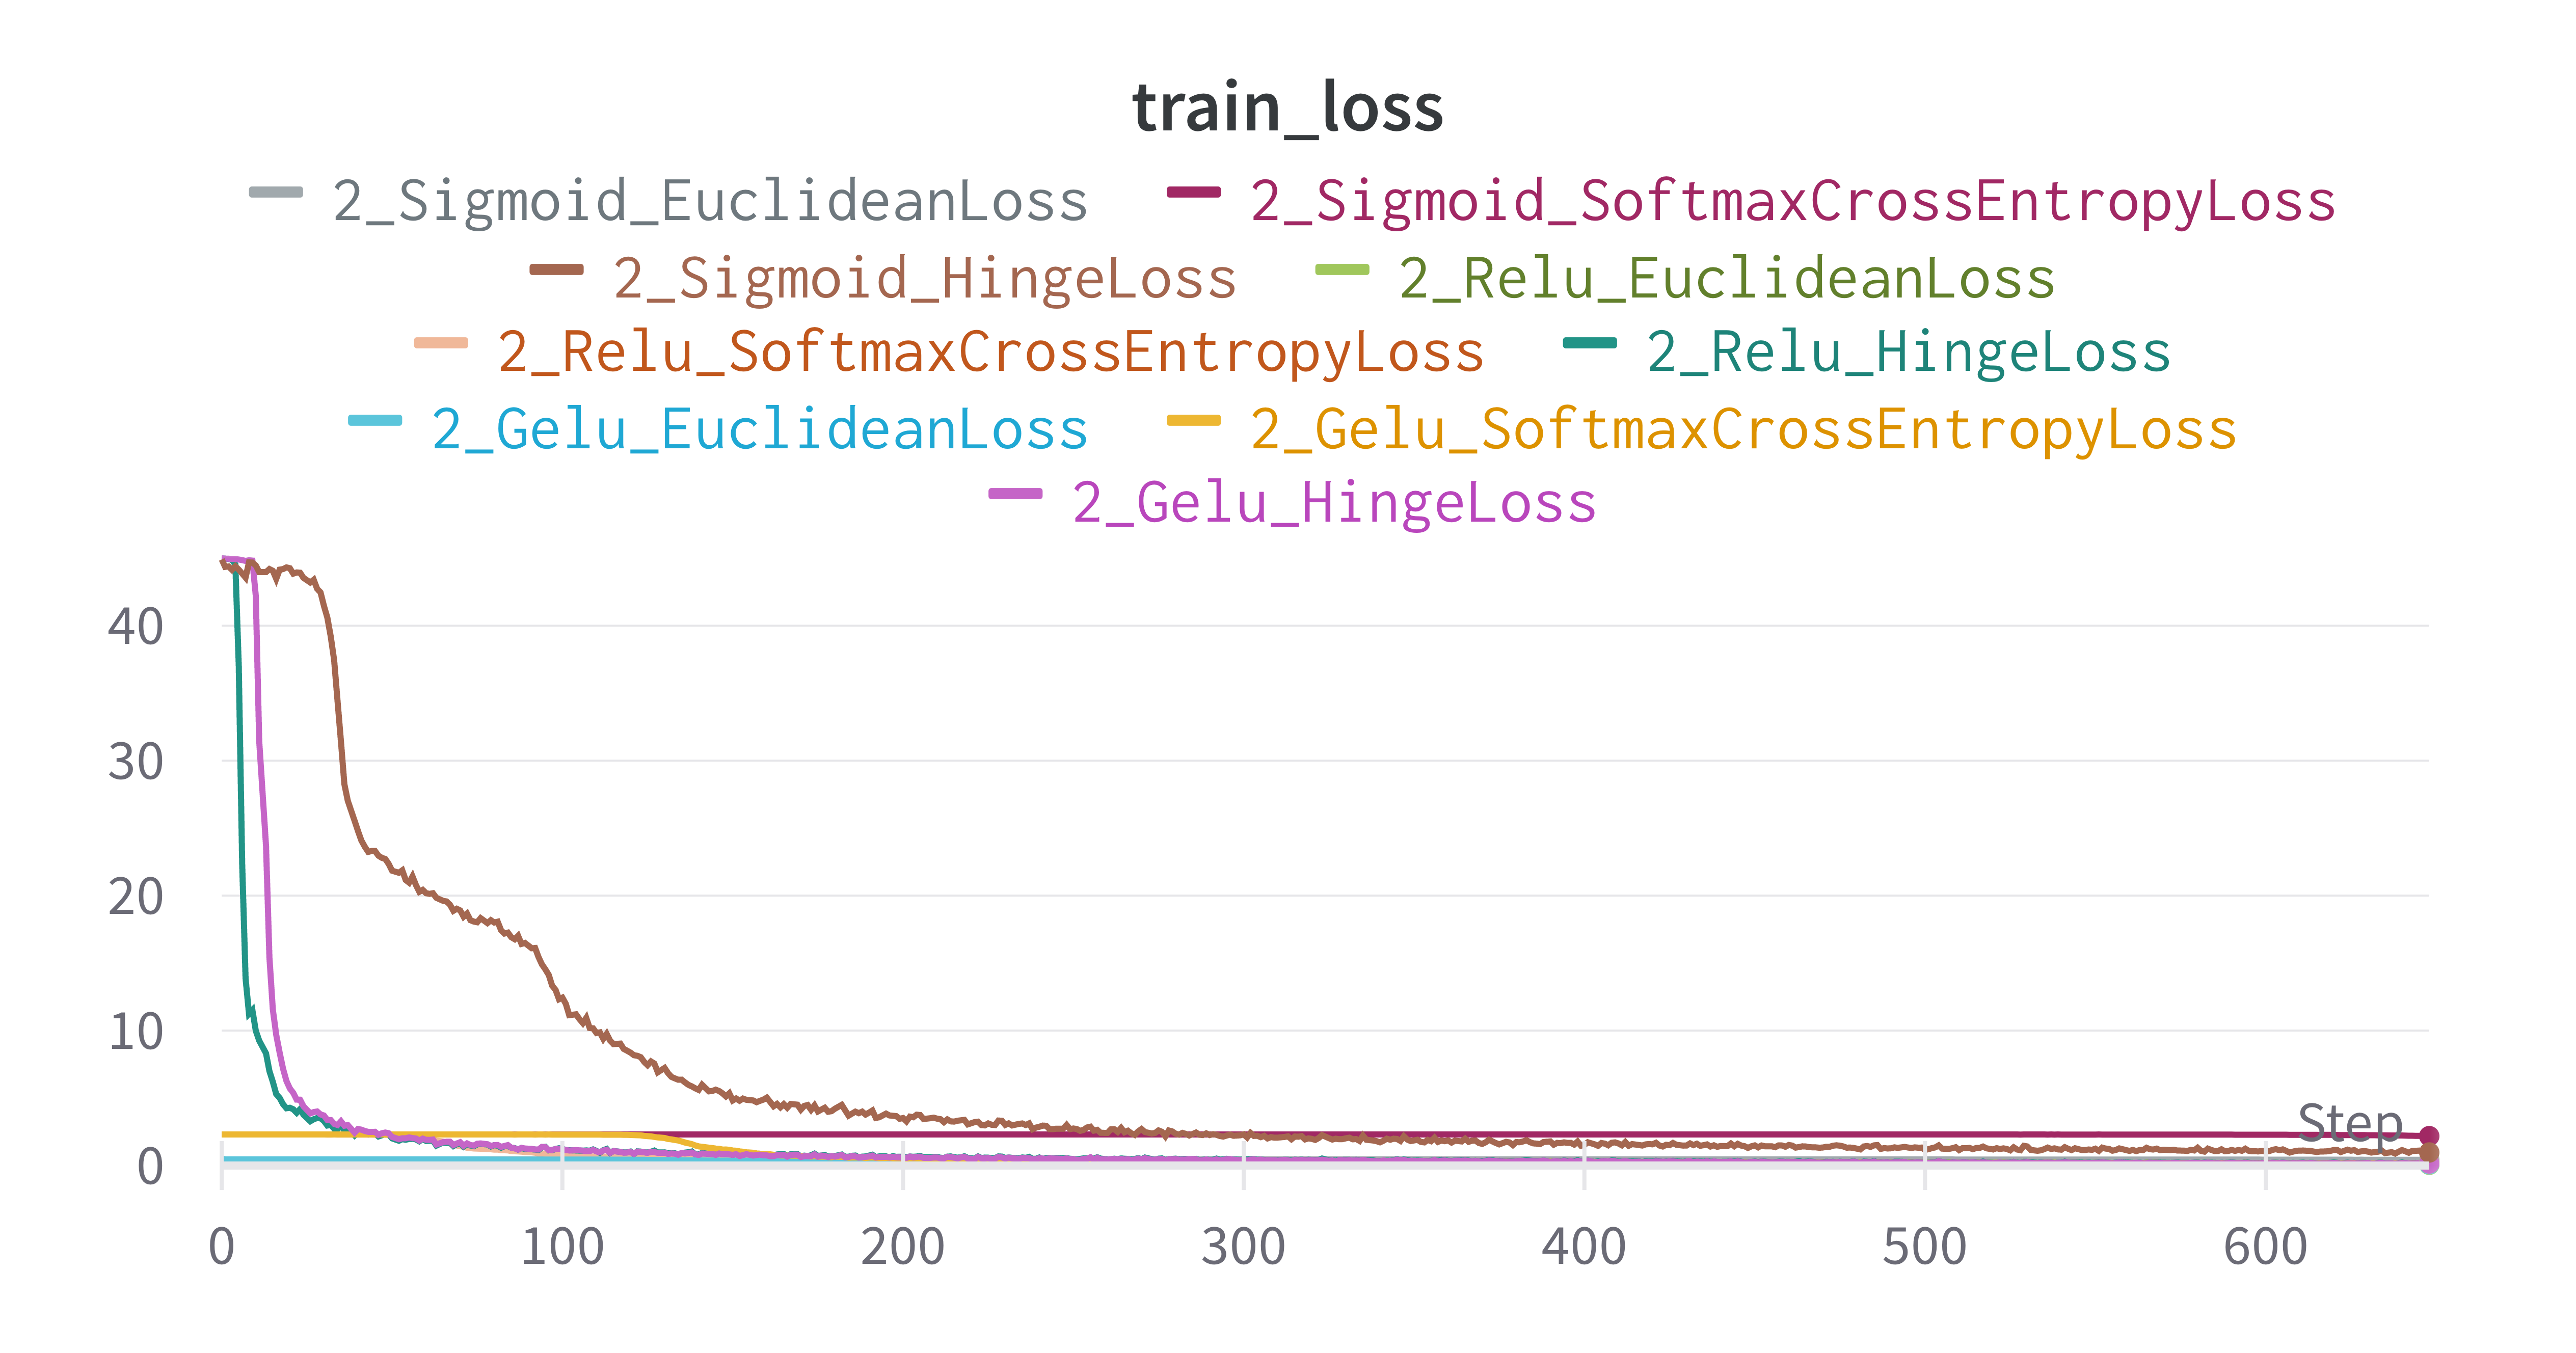
\includegraphics[width=1\textwidth]{../pics/双层实验-train_loss.png}
		\caption{双隐藏层 train loss}
	\end{subfigure}
	\begin{subfigure}{0.475\textwidth}
		\centering
		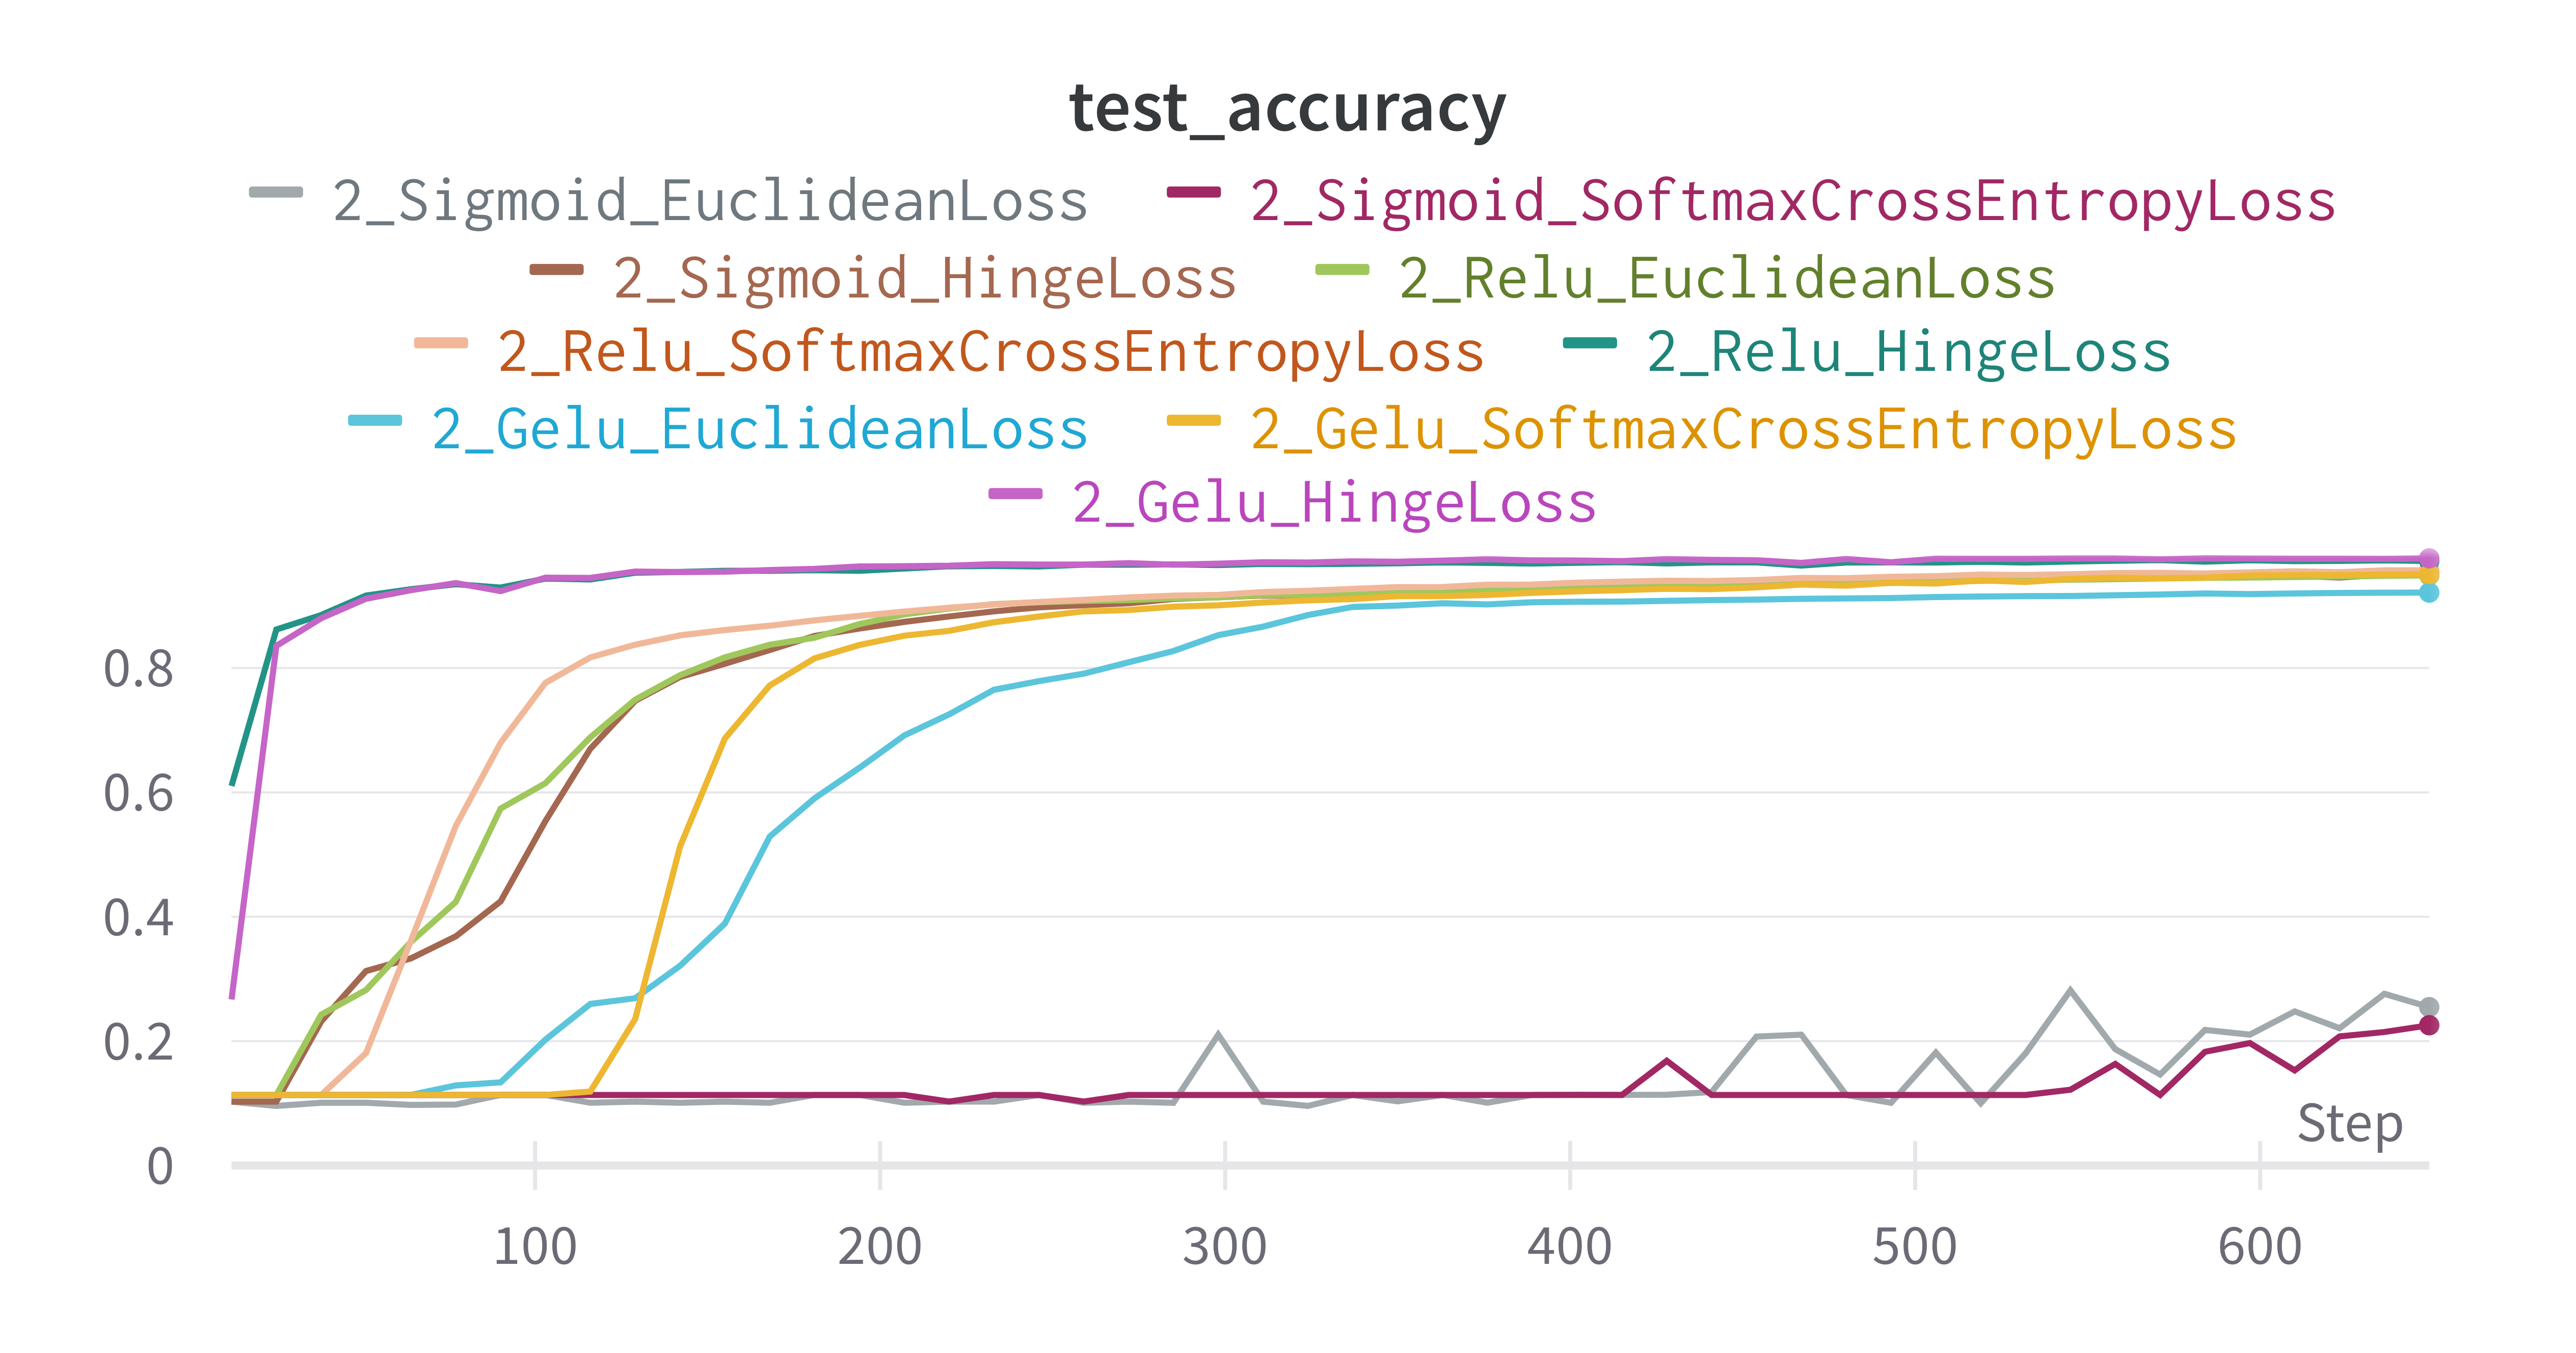
\includegraphics[width=1\textwidth]{../pics/双层实验-test_acc.png}
		\caption{双隐藏层 test accuracy}
	\end{subfigure}
	\begin{subfigure}{0.475\textwidth}
		\centering
		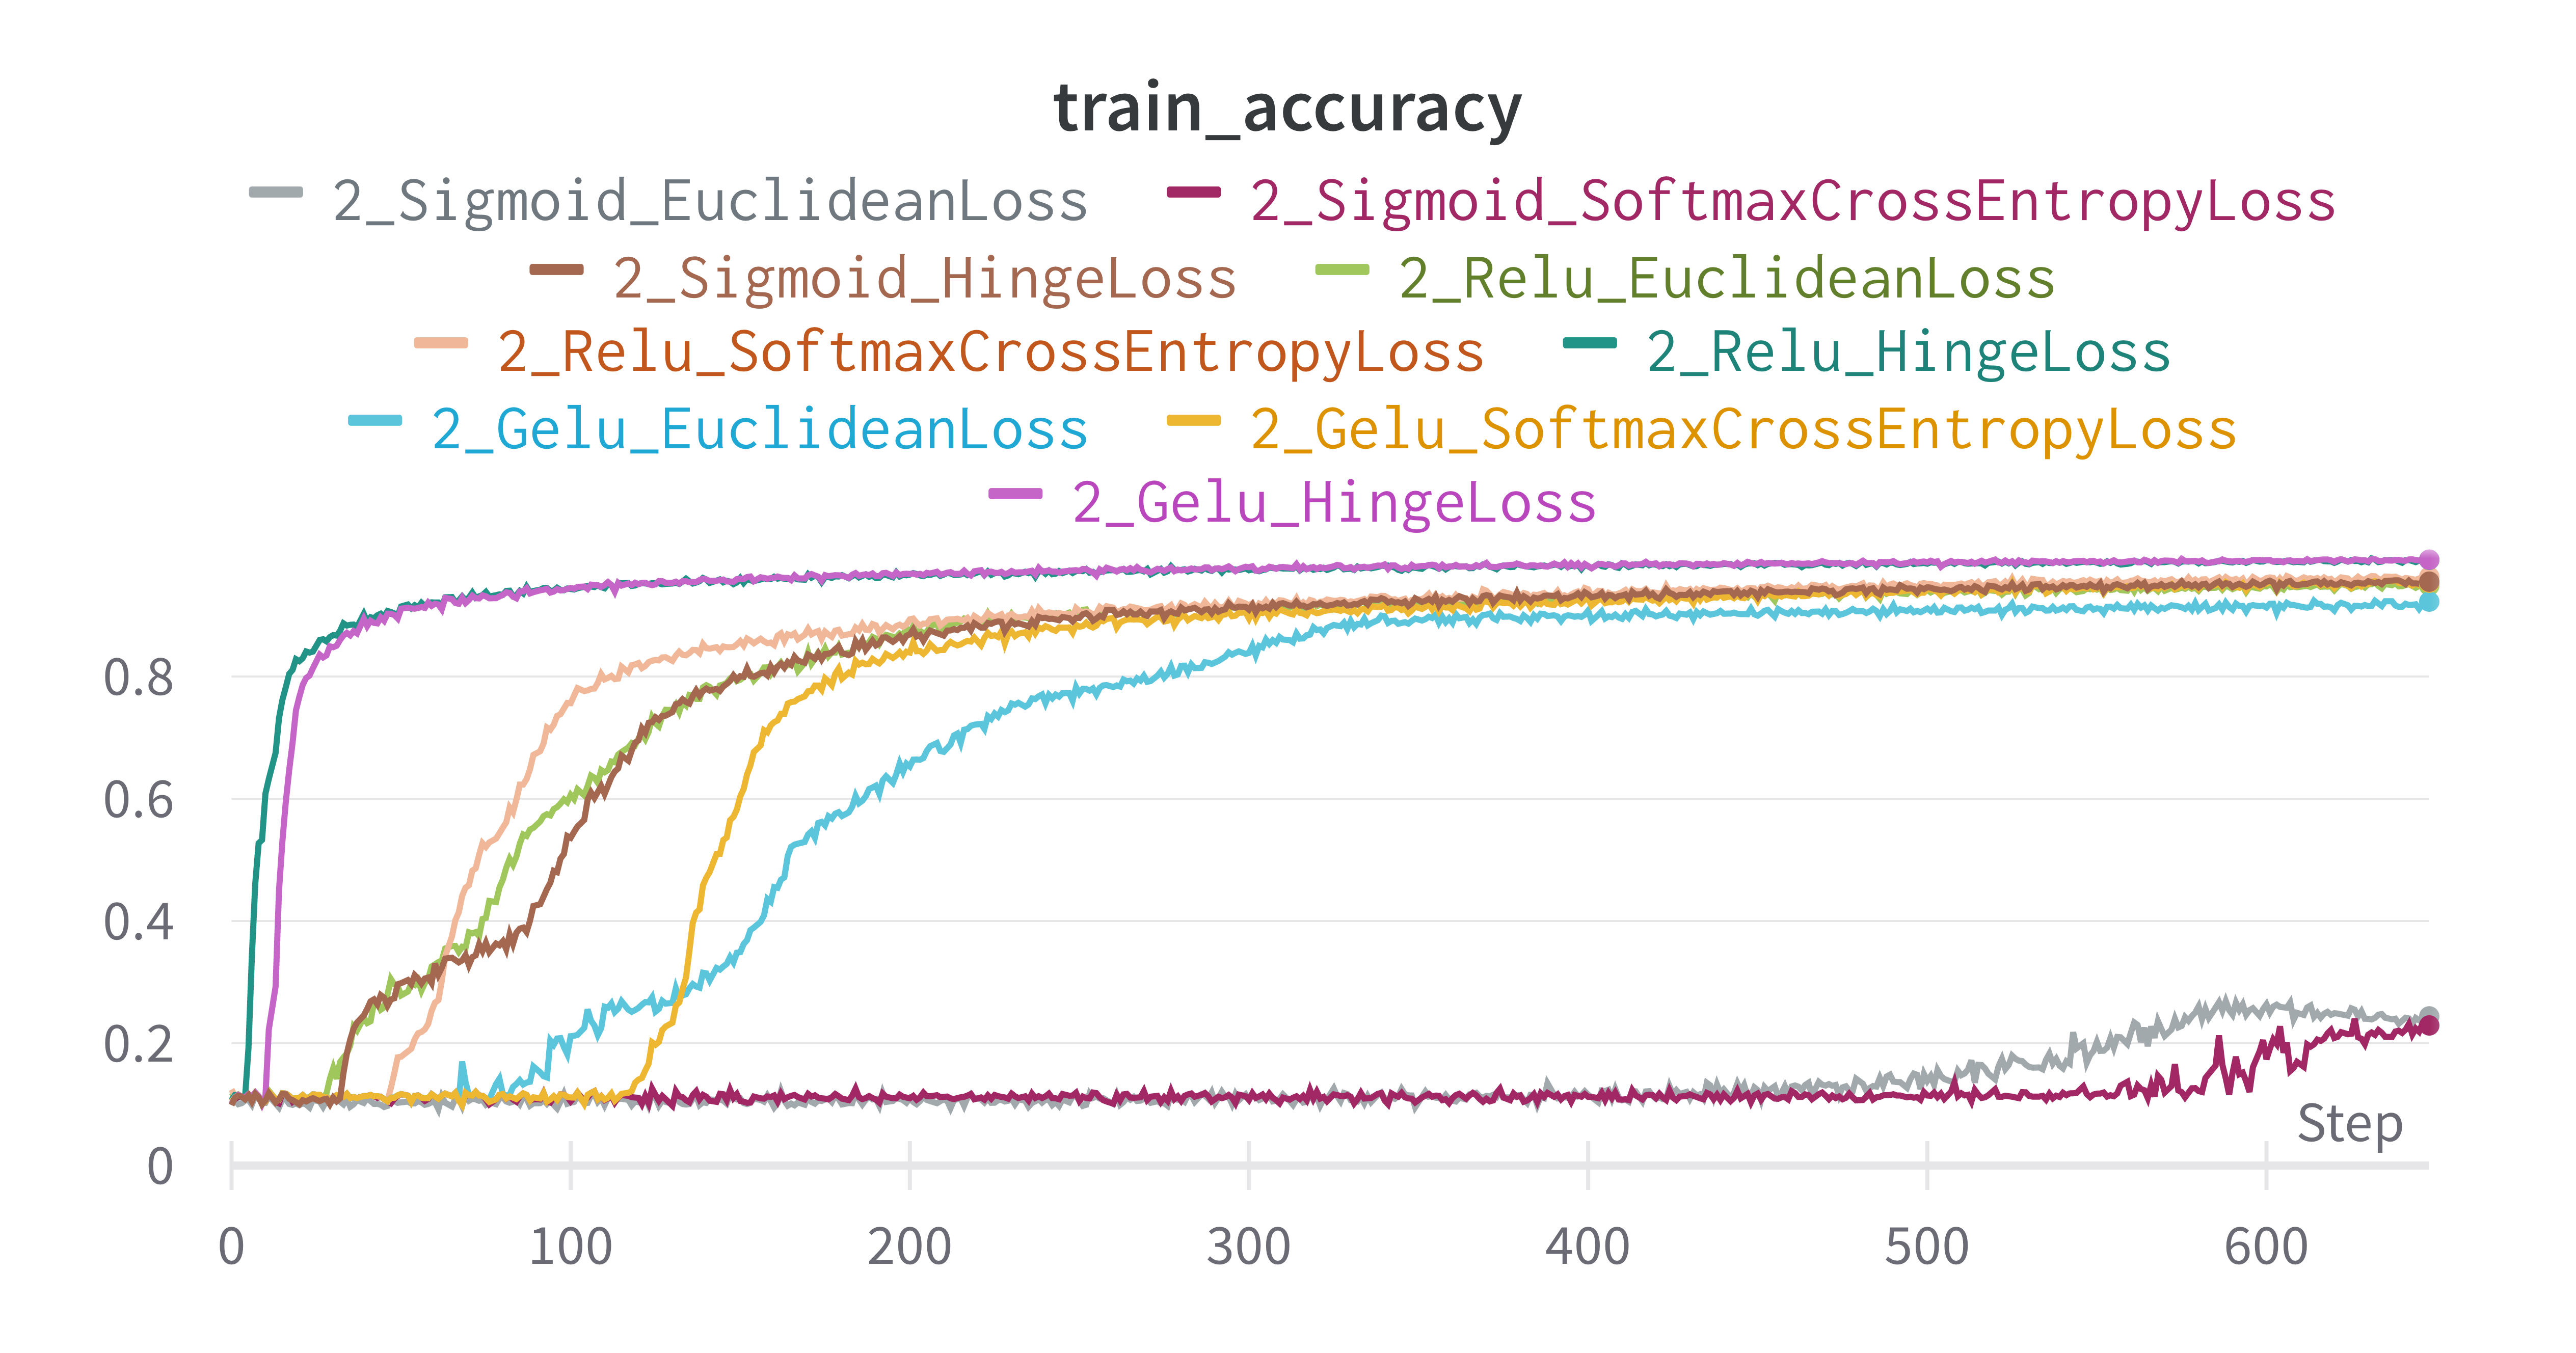
\includegraphics[width=1\textwidth]{../pics/双层实验-train_acc.png}
		\caption{双隐藏层 train accuracy}
	\end{subfigure}
	\caption{双隐藏层实验效果}
	\label{fig:6}
\end{figure}

此外,注意到实际上双隐藏层时,某些模型设定并不能成功训练。考虑到训练失败的设定是 2\_Sigmoid\_SoftmaxCrossEntropy 和 2\_Sigmoid\_Euclidean,而 2\_Sigmoid\_Hinge 成功训练。\\
叠加双层的 Sigmoid 作为激活函数,可能会存在非常严重的梯度消失问题,而只有表达力更强的 Hinge 能够得到训练,这也符合预期。\\
当然,这里所指的不能成功训练是基于基础实验的超参数设计而言的,实际上将学习率从 1e-2 提高到 1 即可让 2\_Sigmoid\_SoftmaxCrossEntropy 成功训练;这也符合预期,因为提高学习率也是对抗梯度衰减的一大方法。
基于此,扩展实验中对学习率的调节便是基于 2\_Sigmoid\_SoftmaxCrossEntropy 而展开。而 2\_Sigmoid\_Euclidean 设定即是调整了学习率,依然难以训练成功。
据此推断,没有使用 residual connection、dropout、batch norm 且没有调整 momentum 的情况下,层数越多 Sigmoid 导致的梯度消失问题越严重,劣势将进一步被放大。

\section{扩展实验}

\subsection{学习率影响}

保留基础实验的参数设定,模型选取 1\_Sigmoid\_EuclideanLoss(图 \ref{fig:7}) 与 2\_Sigmoid\_Softmax(图 \ref{fig:8}),学习率选取为 \{1e-4, 1e-3, 1e-2, 1e-1, 1\},展开学习率对比实验。

\begin{figure}
	\centering
	\begin{subfigure}{0.475\textwidth}
		\centering
		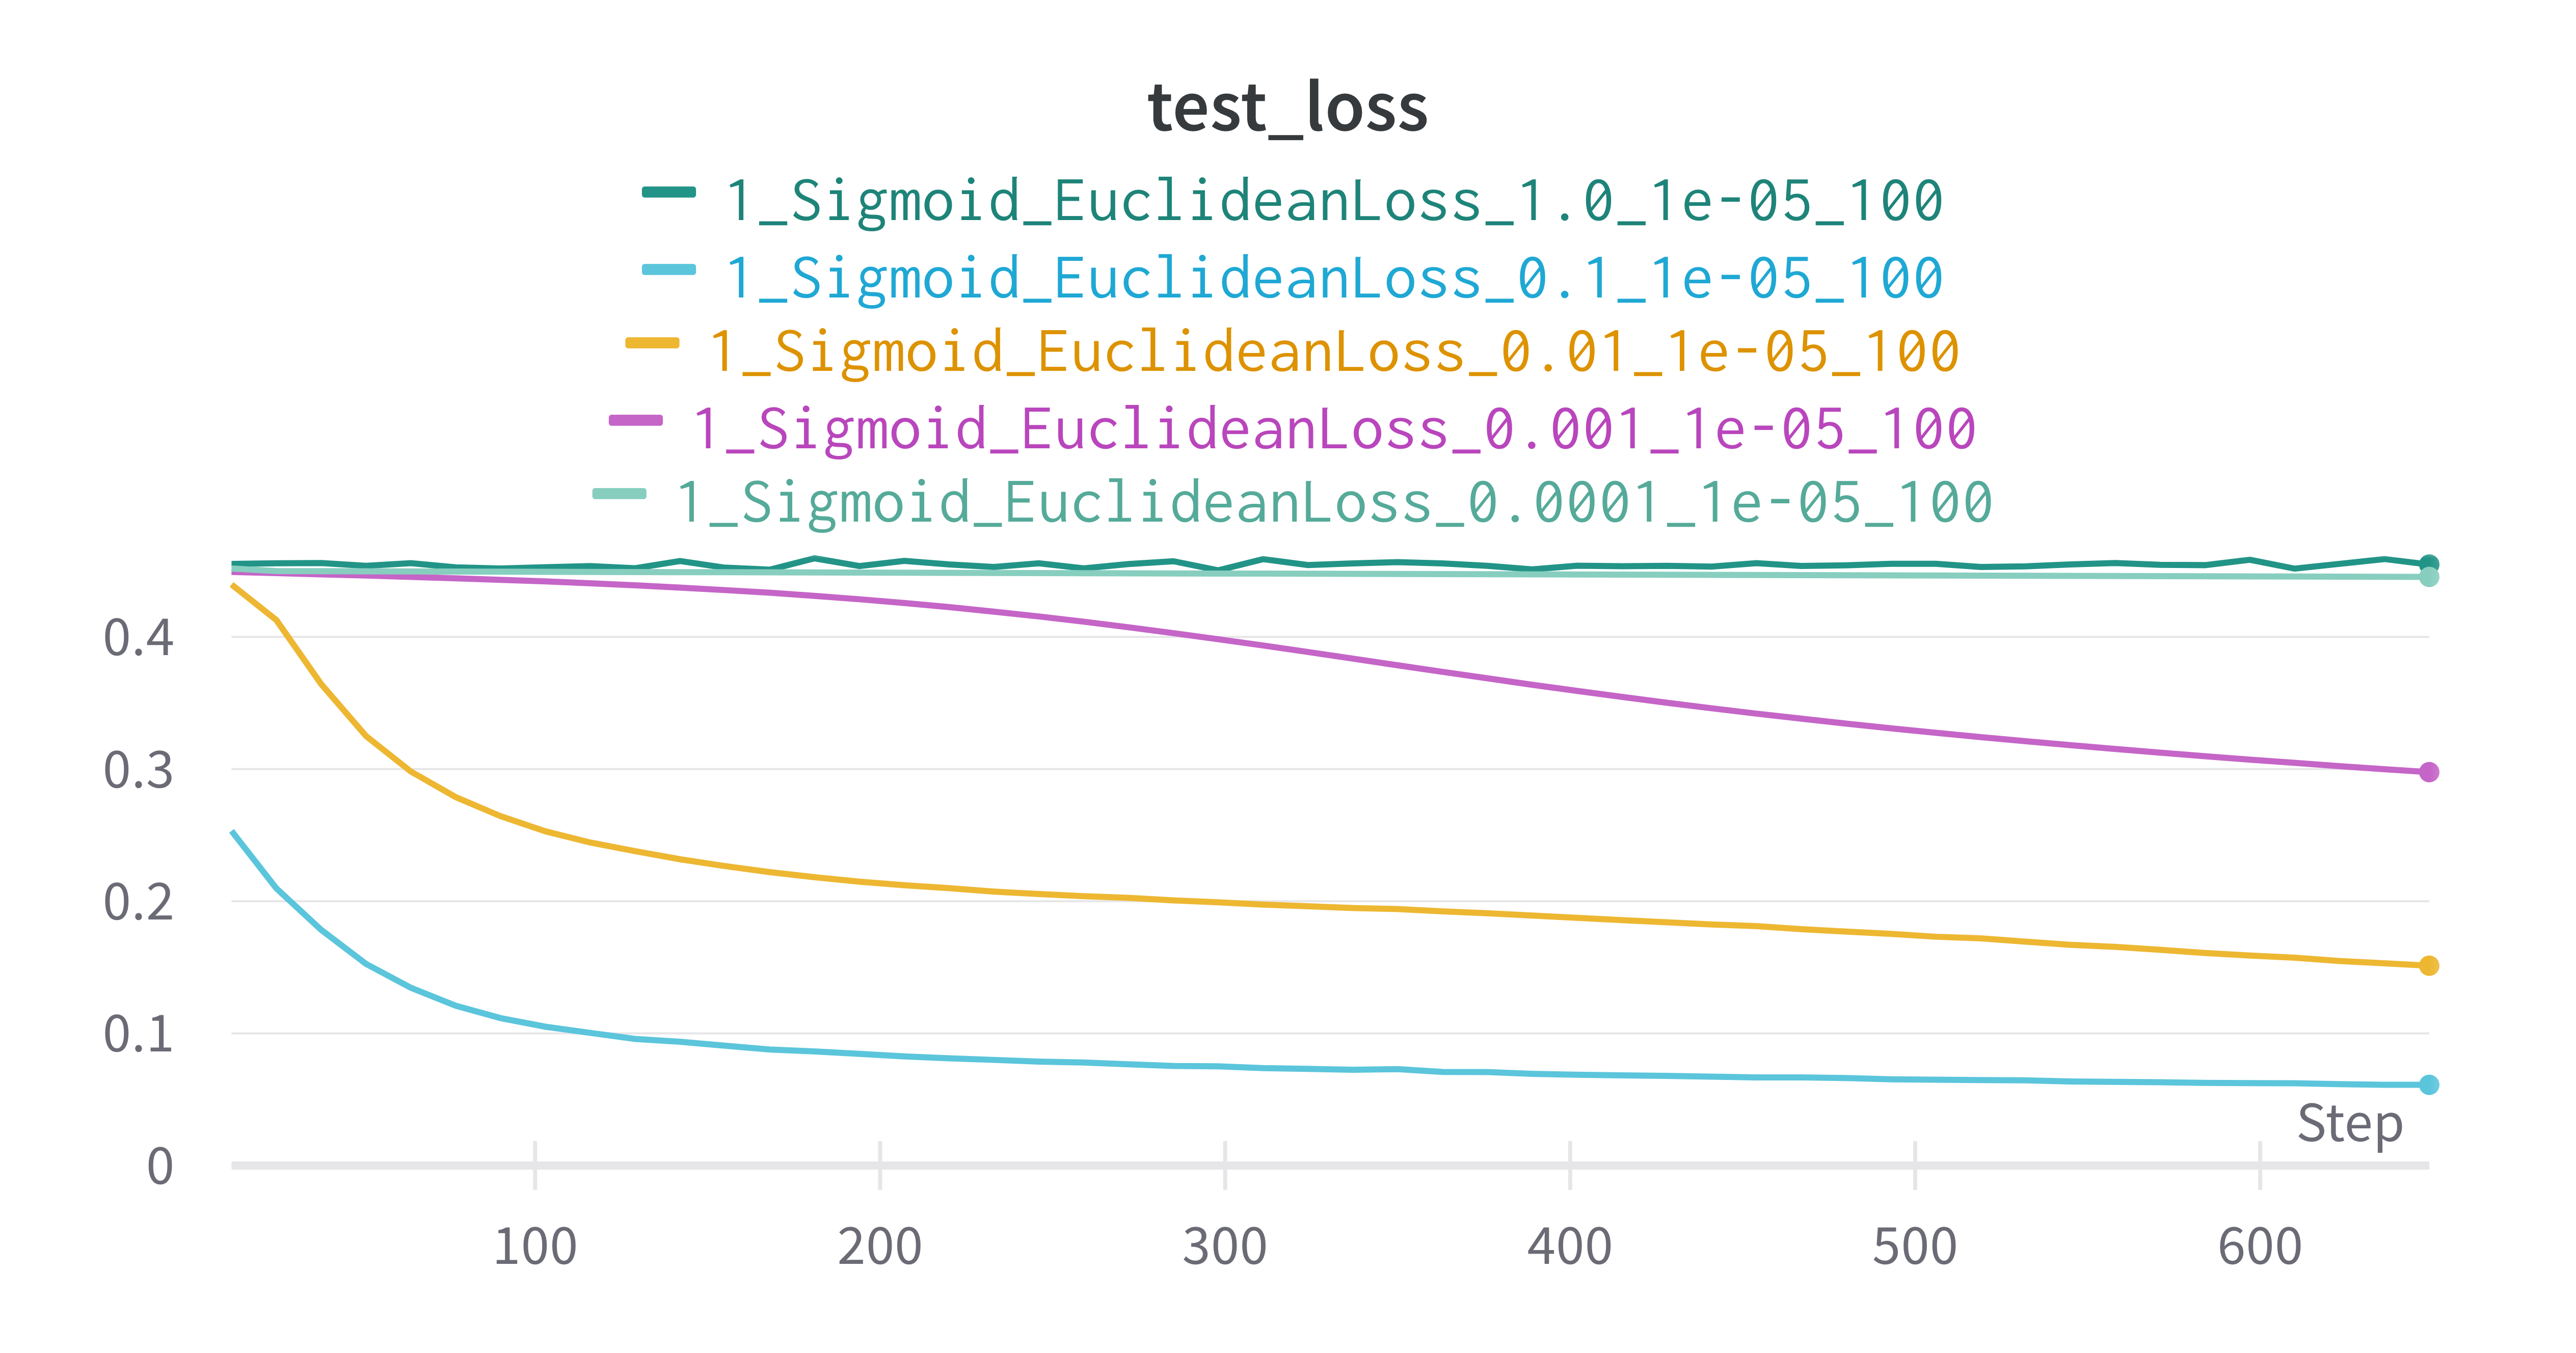
\includegraphics[width=1\textwidth]{../pics/学习率_1_Sigmoid_EuclideanLoss_test_loss.png}
		\caption{1\_Sigmoid\_EuclideanLoss 对比 test loss}
	\end{subfigure}
	\begin{subfigure}{0.475\textwidth}
		\centering
		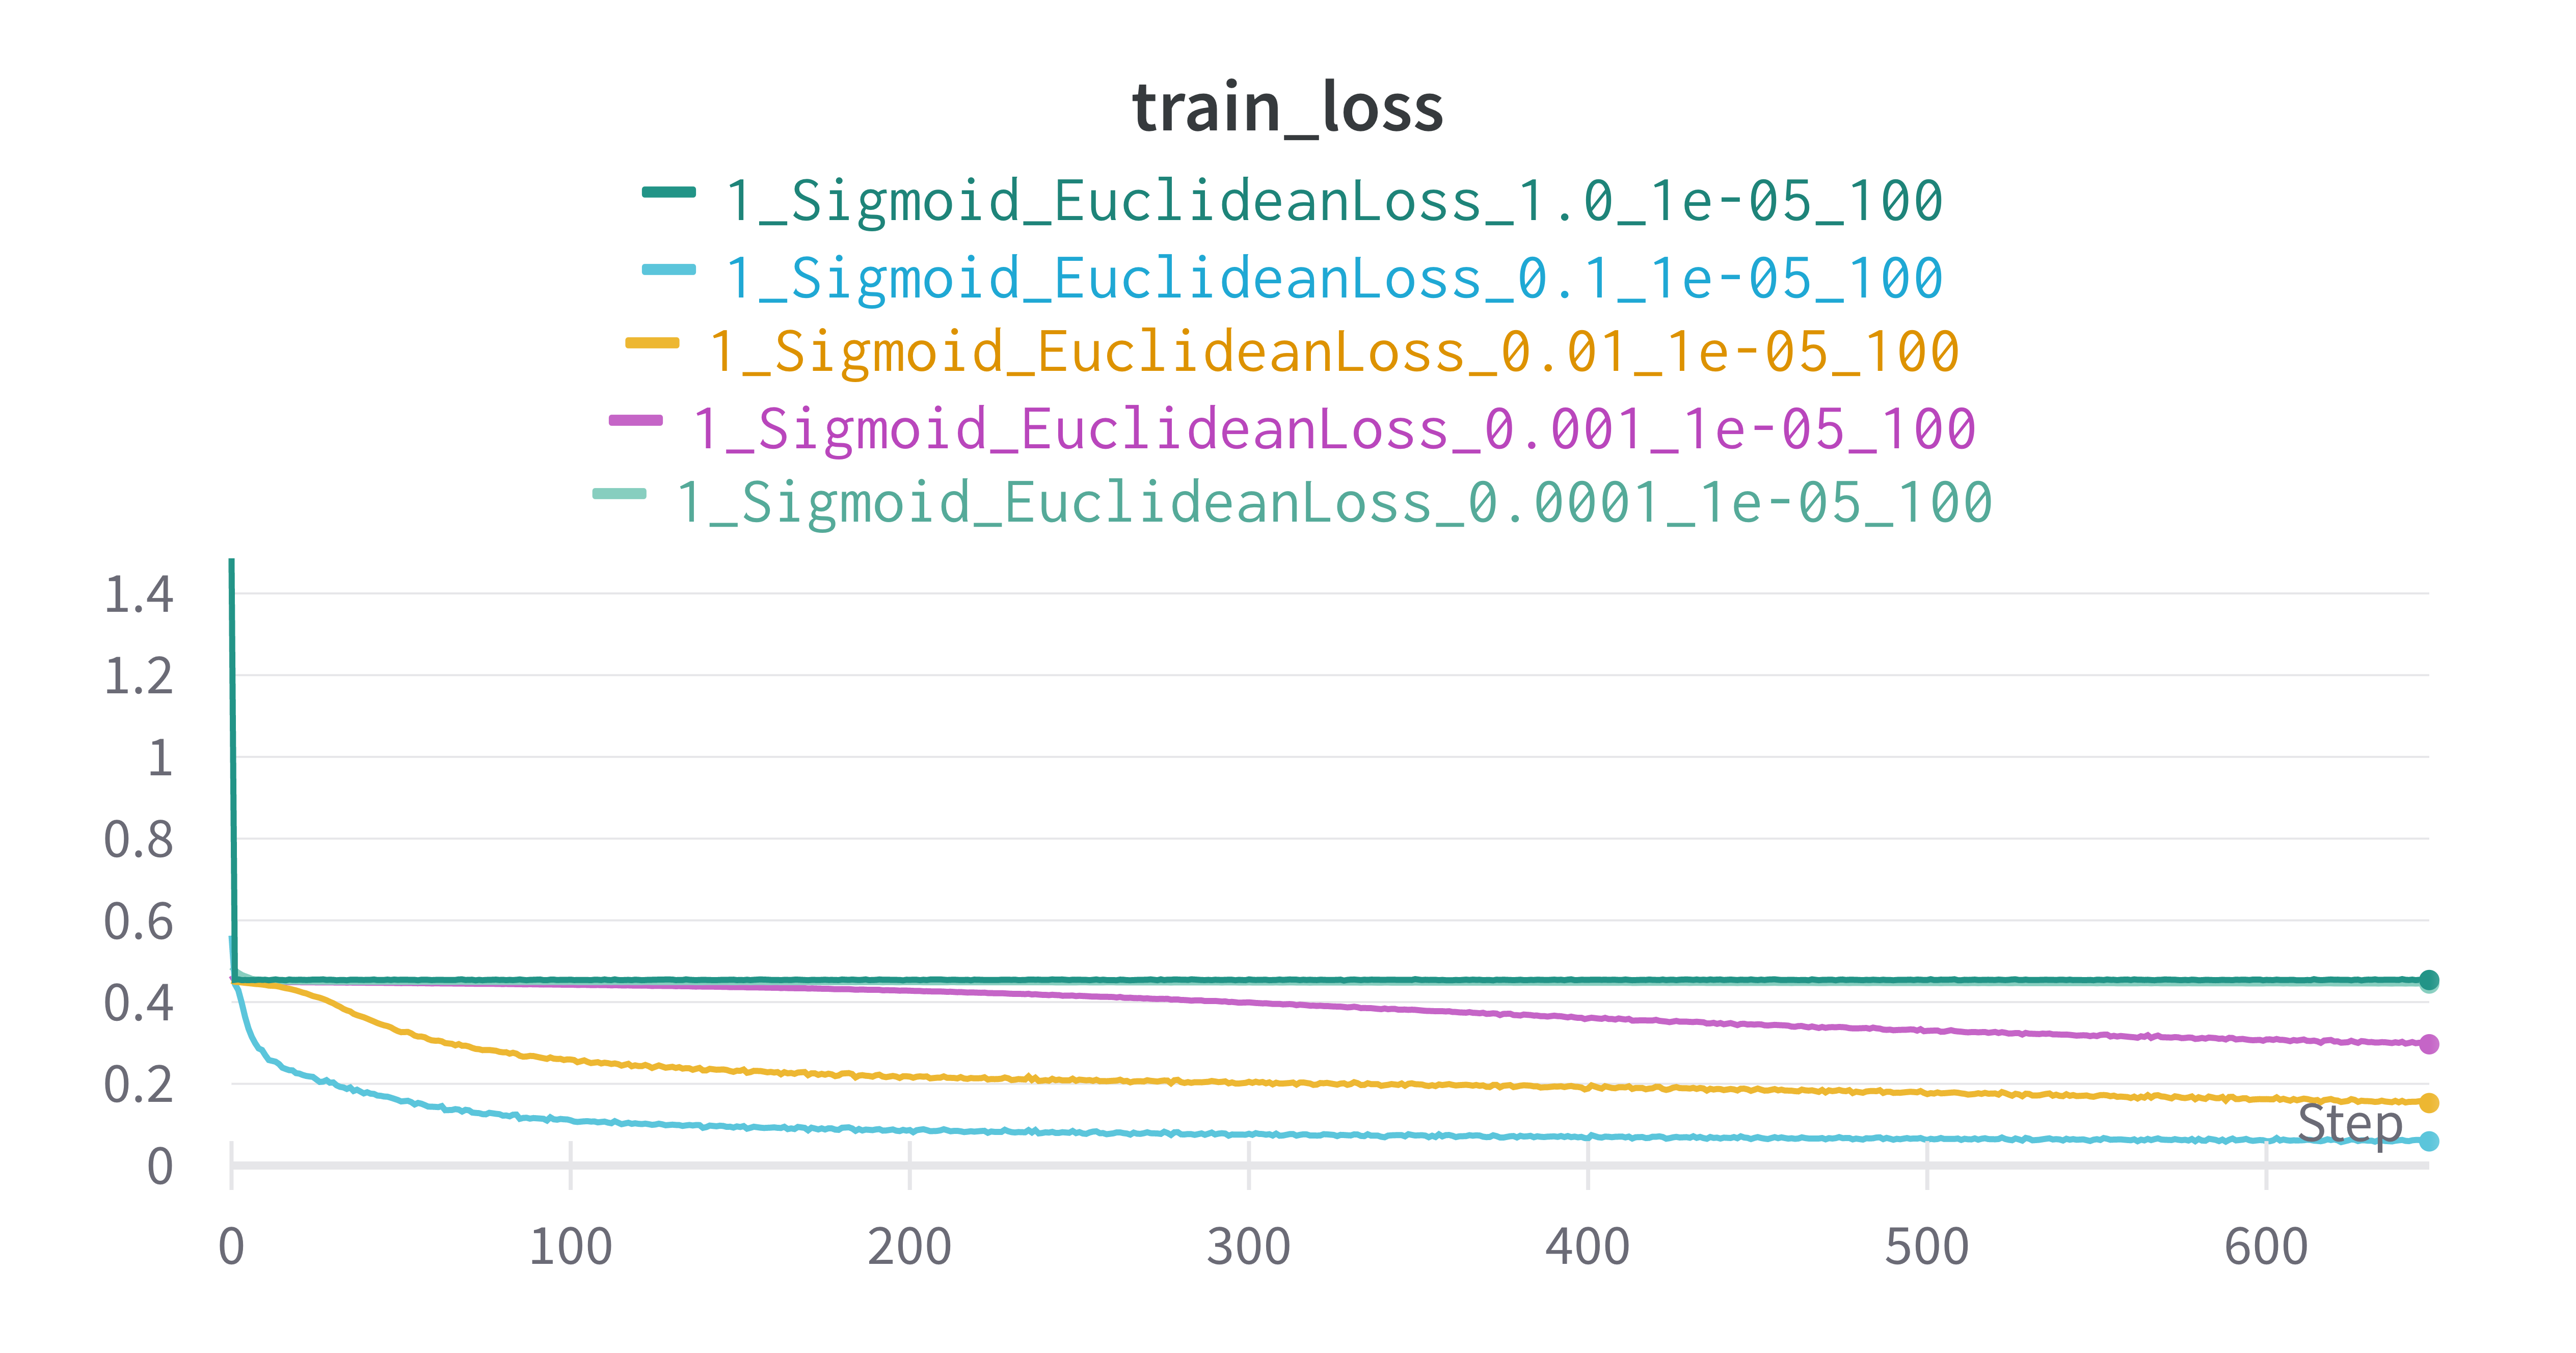
\includegraphics[width=1\textwidth]{../pics/学习率_1_Sigmoid_EuclideanLoss_train_loss.png}
		\caption{1\_Sigmoid\_EuclideanLoss 对比 train loss}
	\end{subfigure}
	\begin{subfigure}{0.475\textwidth}
		\centering
		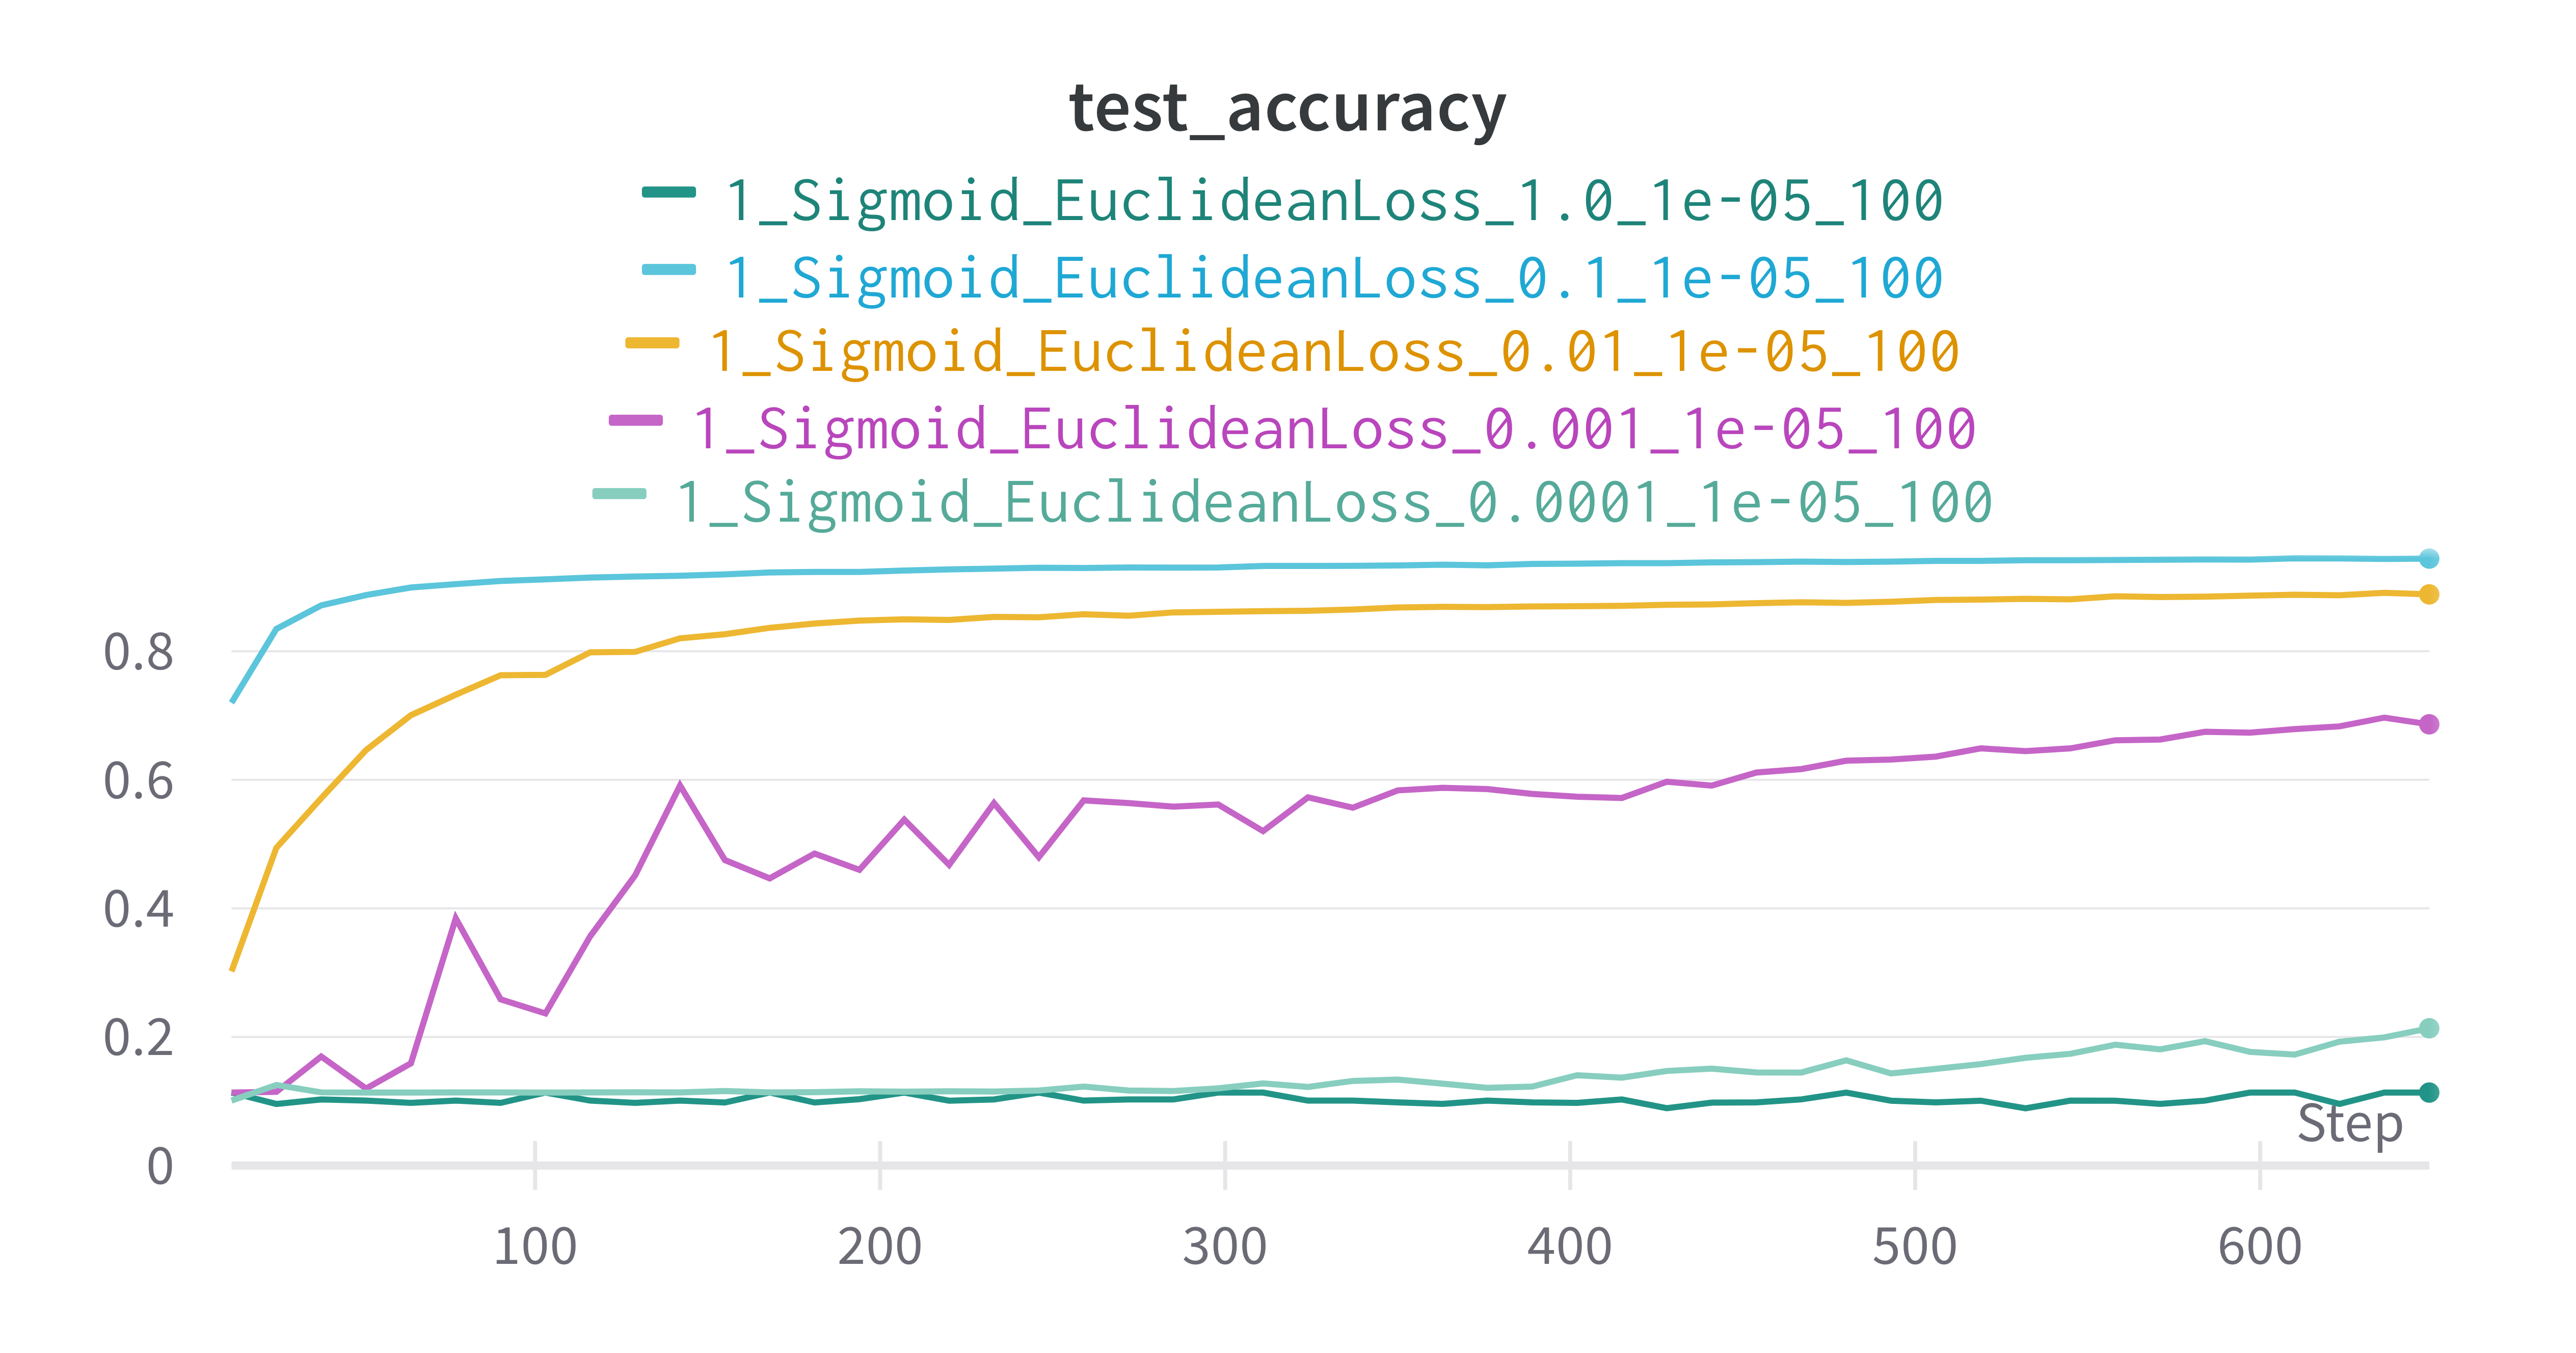
\includegraphics[width=1\textwidth]{../pics/学习率_1_Sigmoid_EuclideanLoss_test_acc.png}
		\caption{1\_Sigmoid\_EuclideanLoss 对比 test accuracy}
	\end{subfigure}
	\begin{subfigure}{0.475\textwidth}
		\centering
		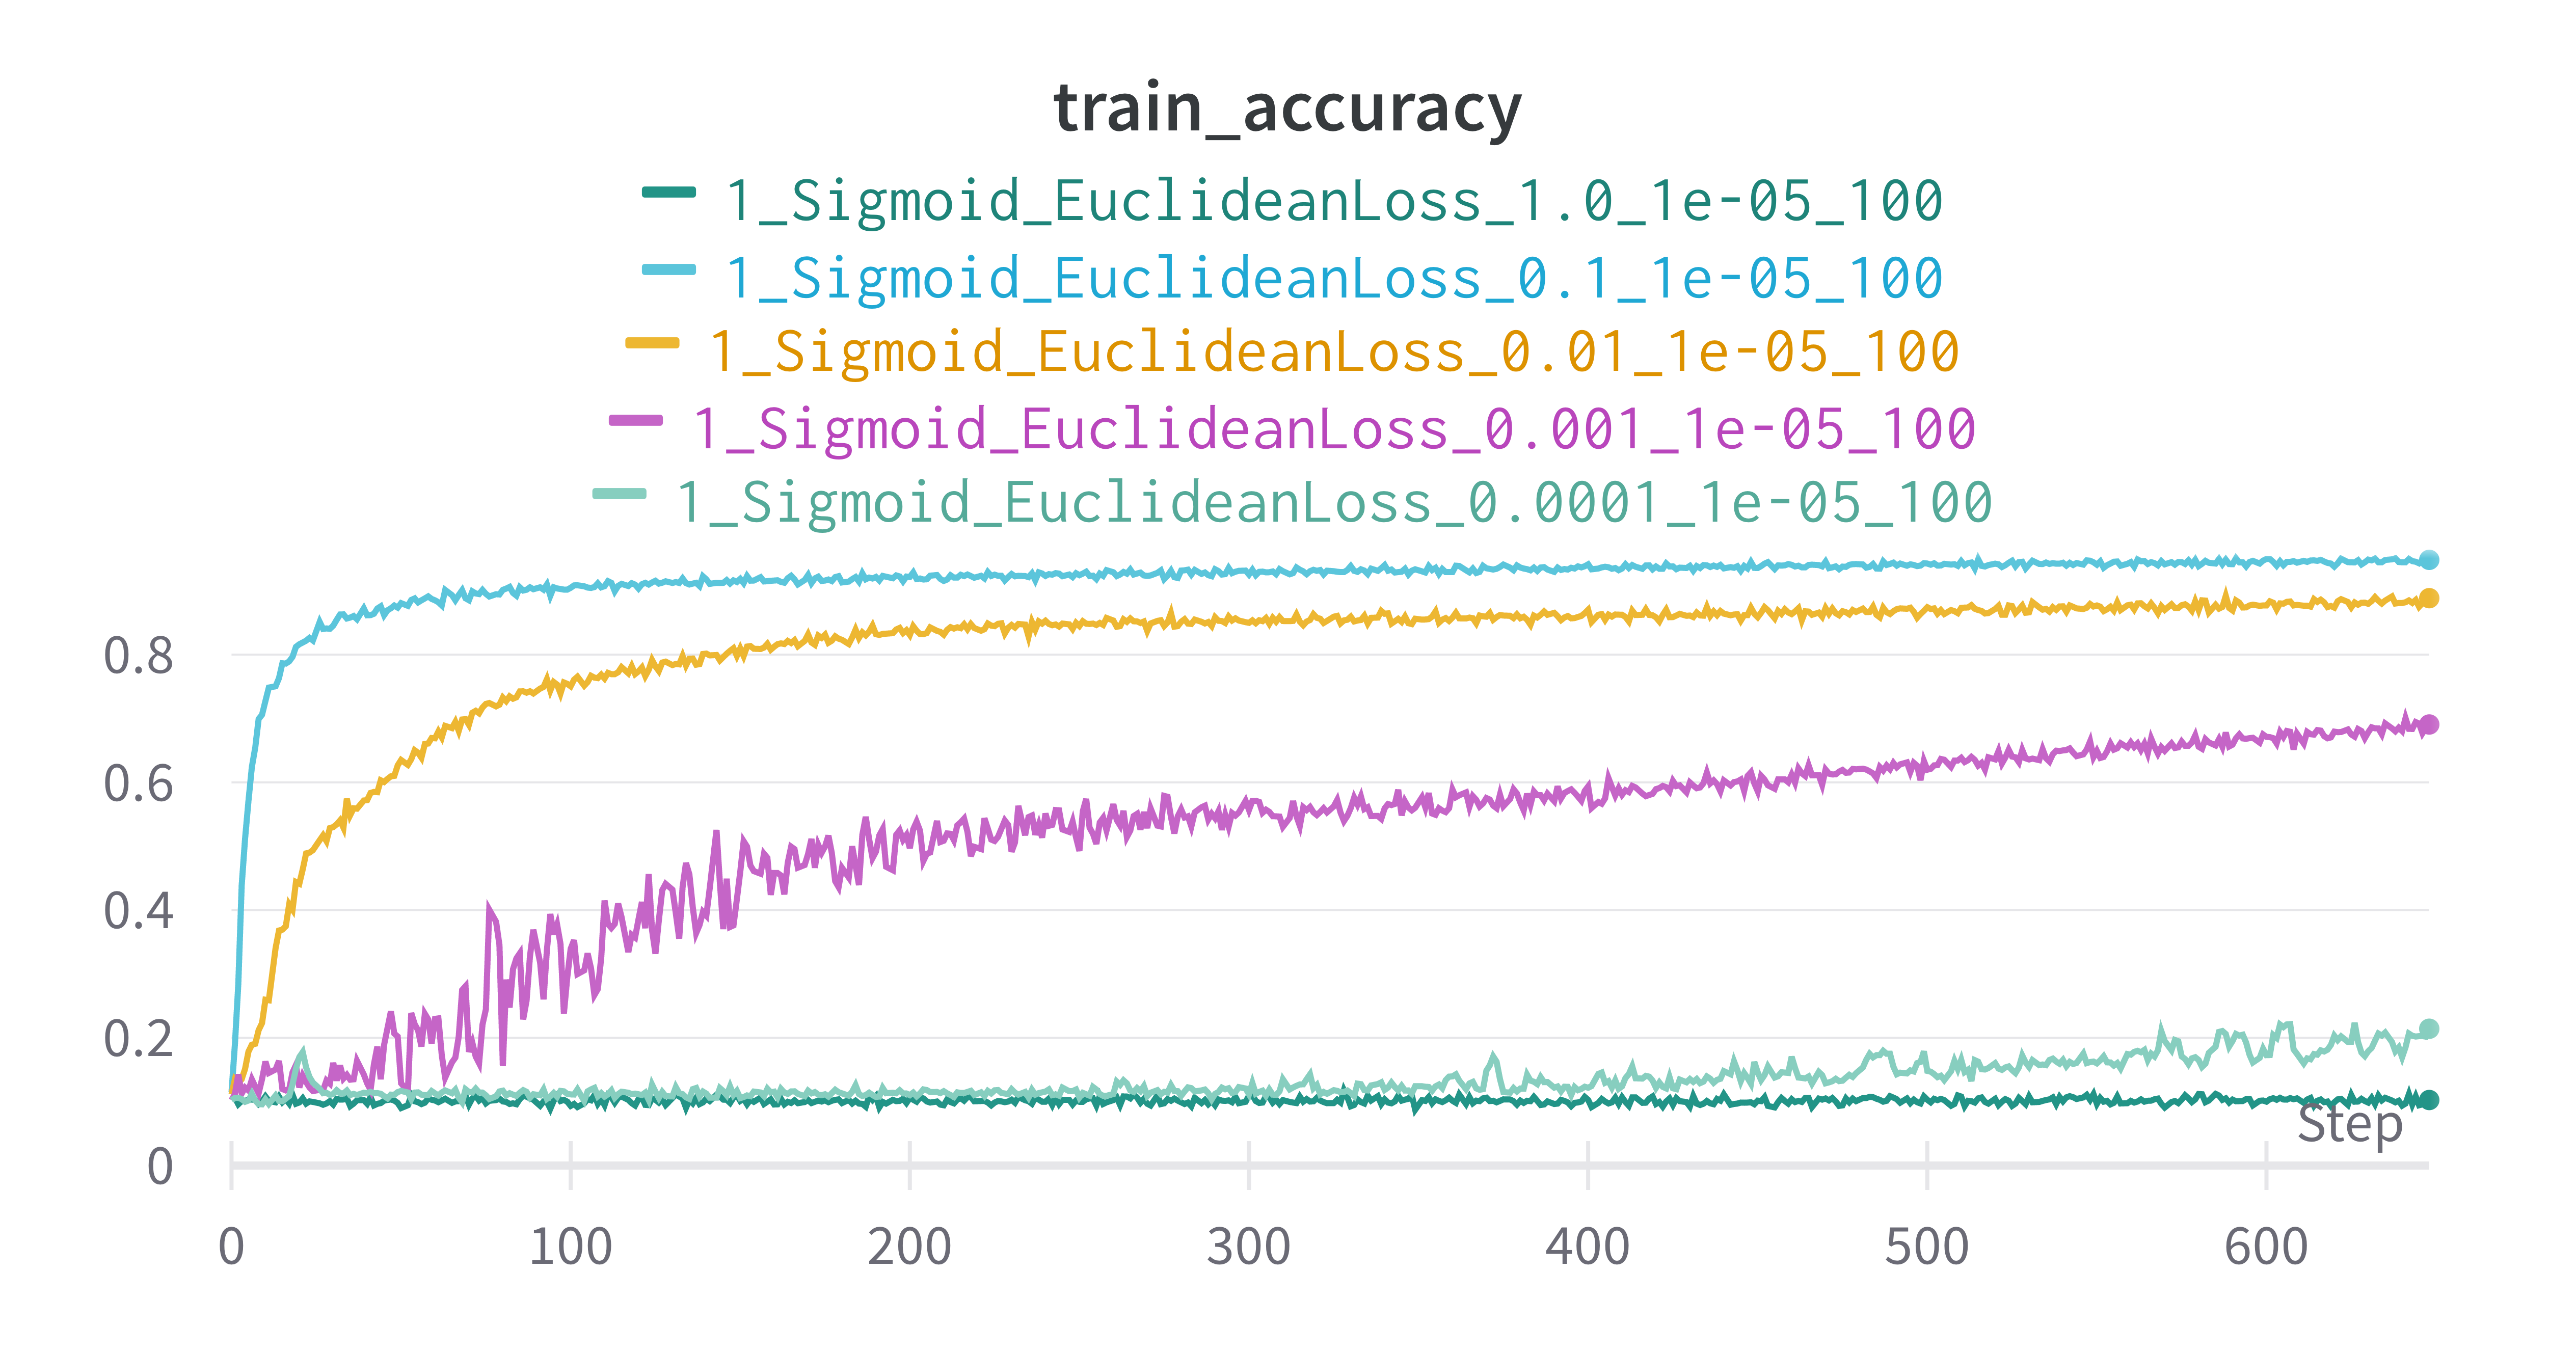
\includegraphics[width=1\textwidth]{../pics/学习率_1_Sigmoid_EuclideanLoss_train_acc.png}
		\caption{1\_Sigmoid\_EuclideanLoss 对比 train accuracy}
	\end{subfigure}
	\caption{基于 1\_Sigmoid\_EuclideanLoss 调节学习率}
	\label{fig:7}
\end{figure}

\begin{figure}[htbp]
	\centering
	\begin{subfigure}{0.475\textwidth}
		\centering
		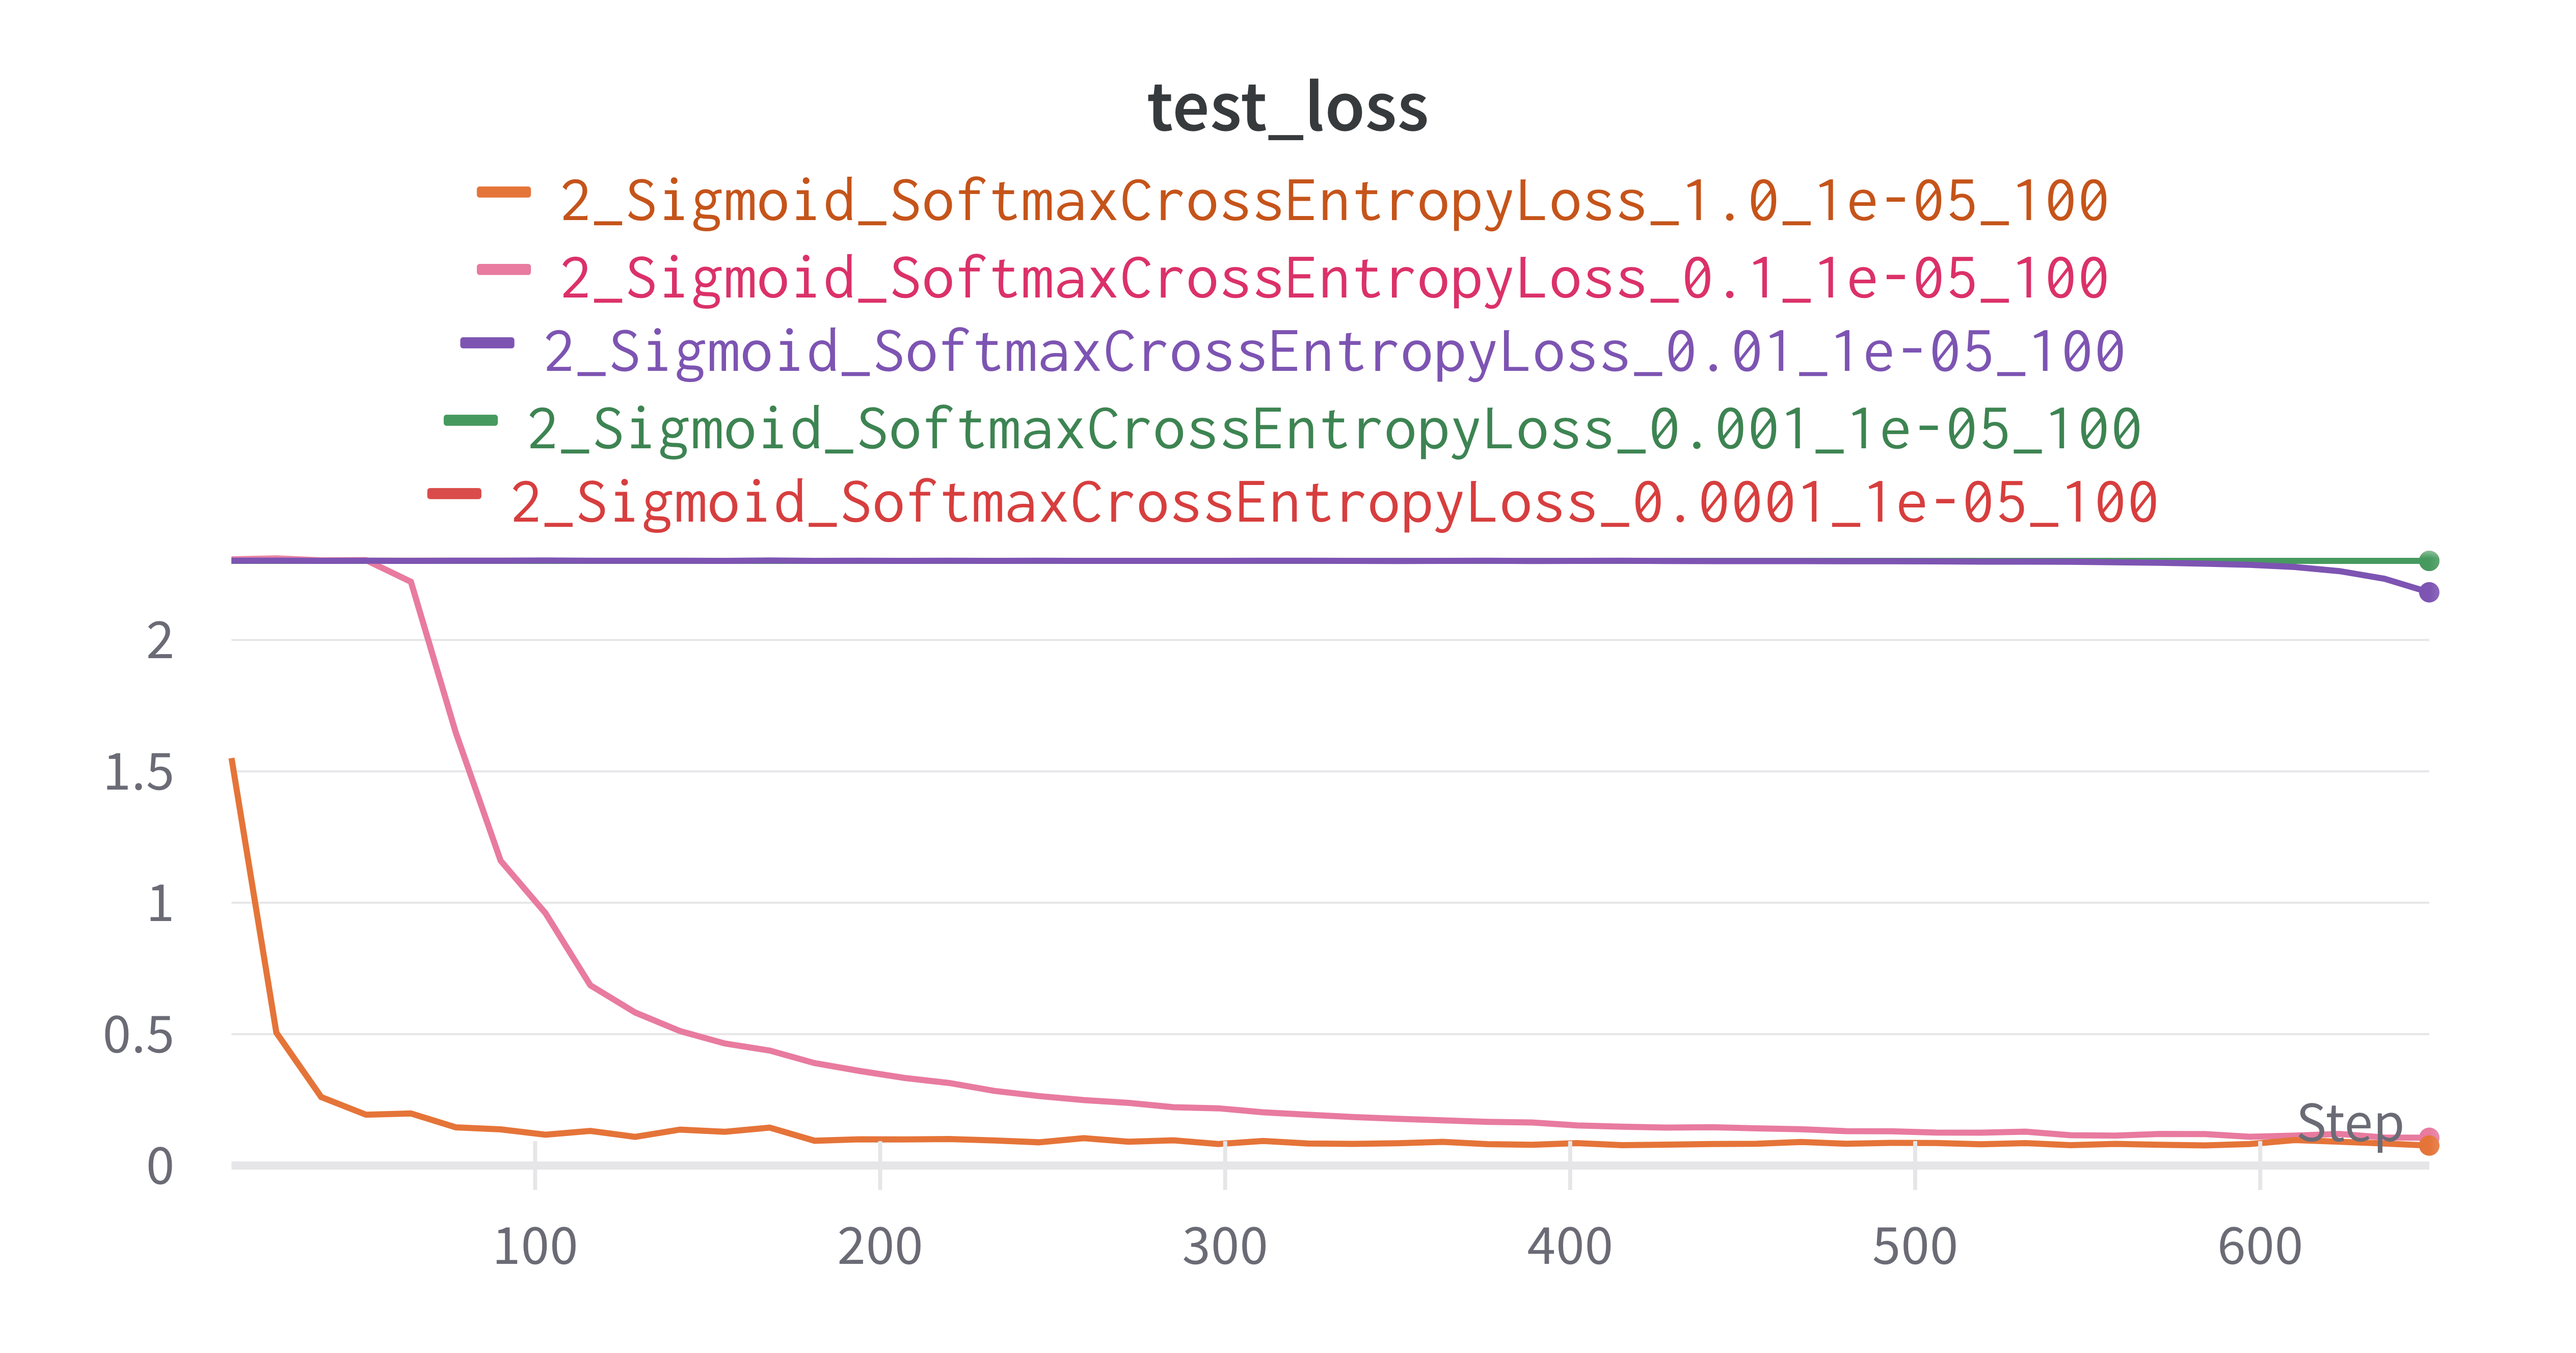
\includegraphics[width=1\textwidth]{../pics/学习率_2_Sigmoid_Softmax_test_loss.png}
		\caption{2\_Sigmoid\_Softmax 对比 test loss}
	\end{subfigure}
	\begin{subfigure}{0.475\textwidth}
		\centering
		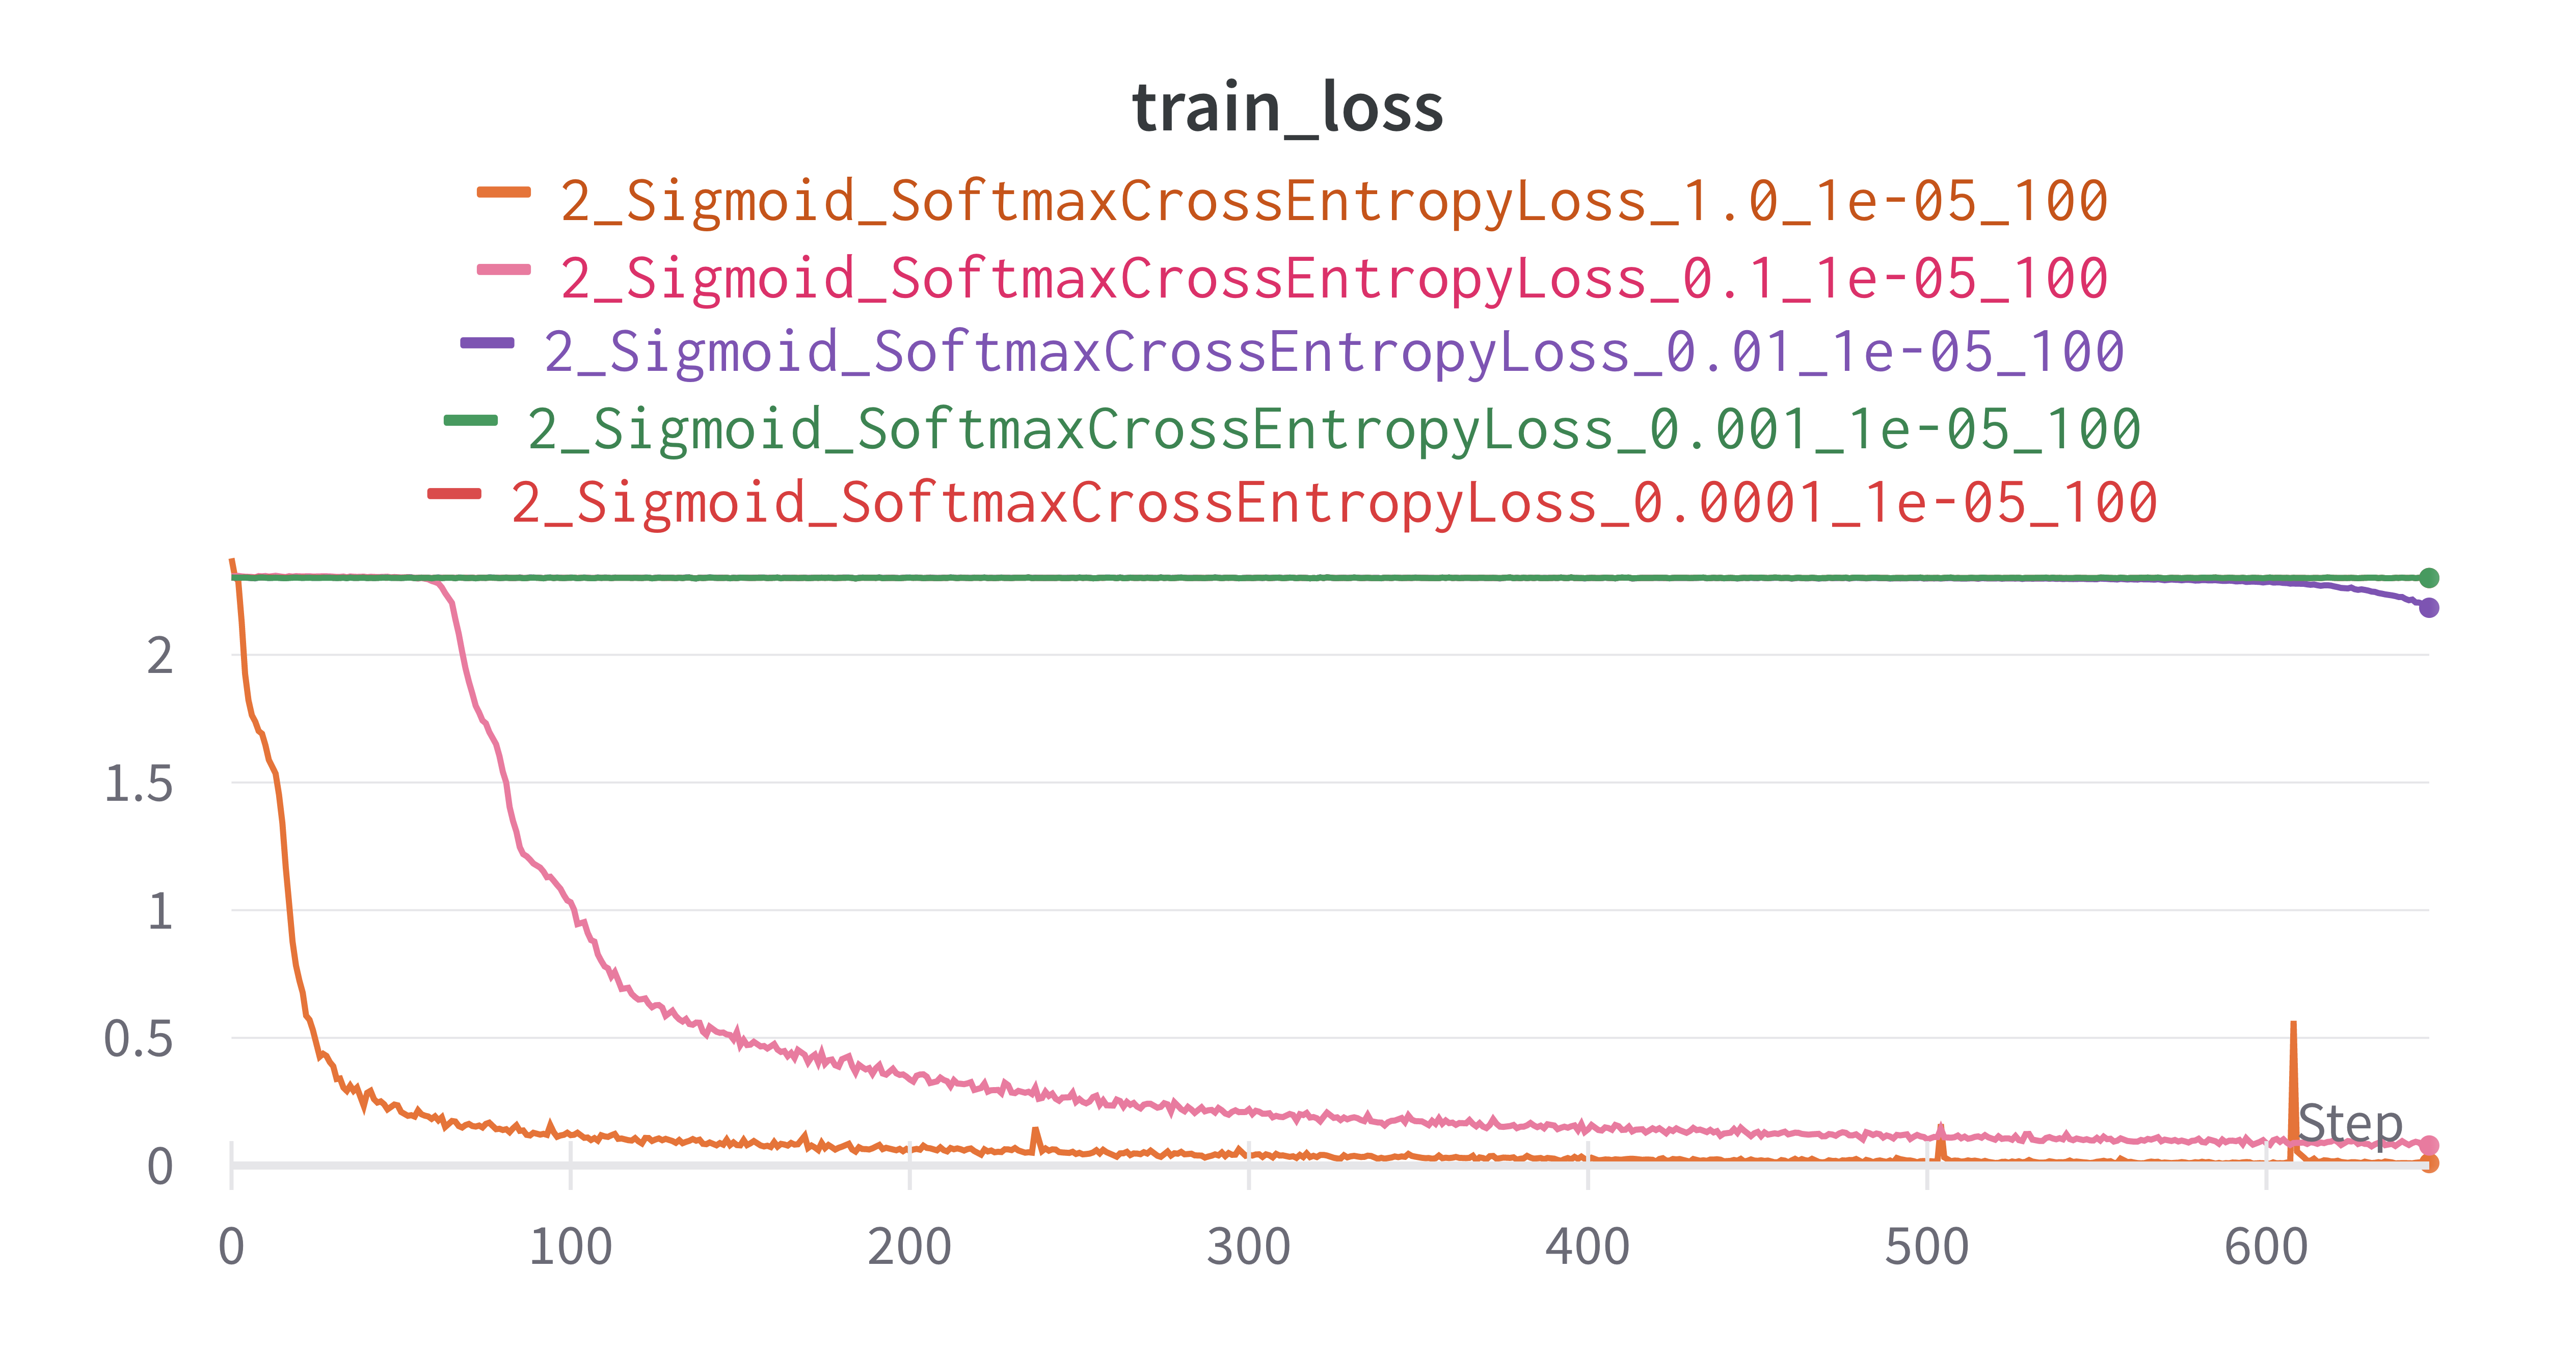
\includegraphics[width=1\textwidth]{../pics/学习率_2_Sigmoid_Softmax_train_loss.png}
		\caption{2\_Sigmoid\_Softmax 对比 train loss}
	\end{subfigure}
	\begin{subfigure}{0.475\textwidth}
		\centering
		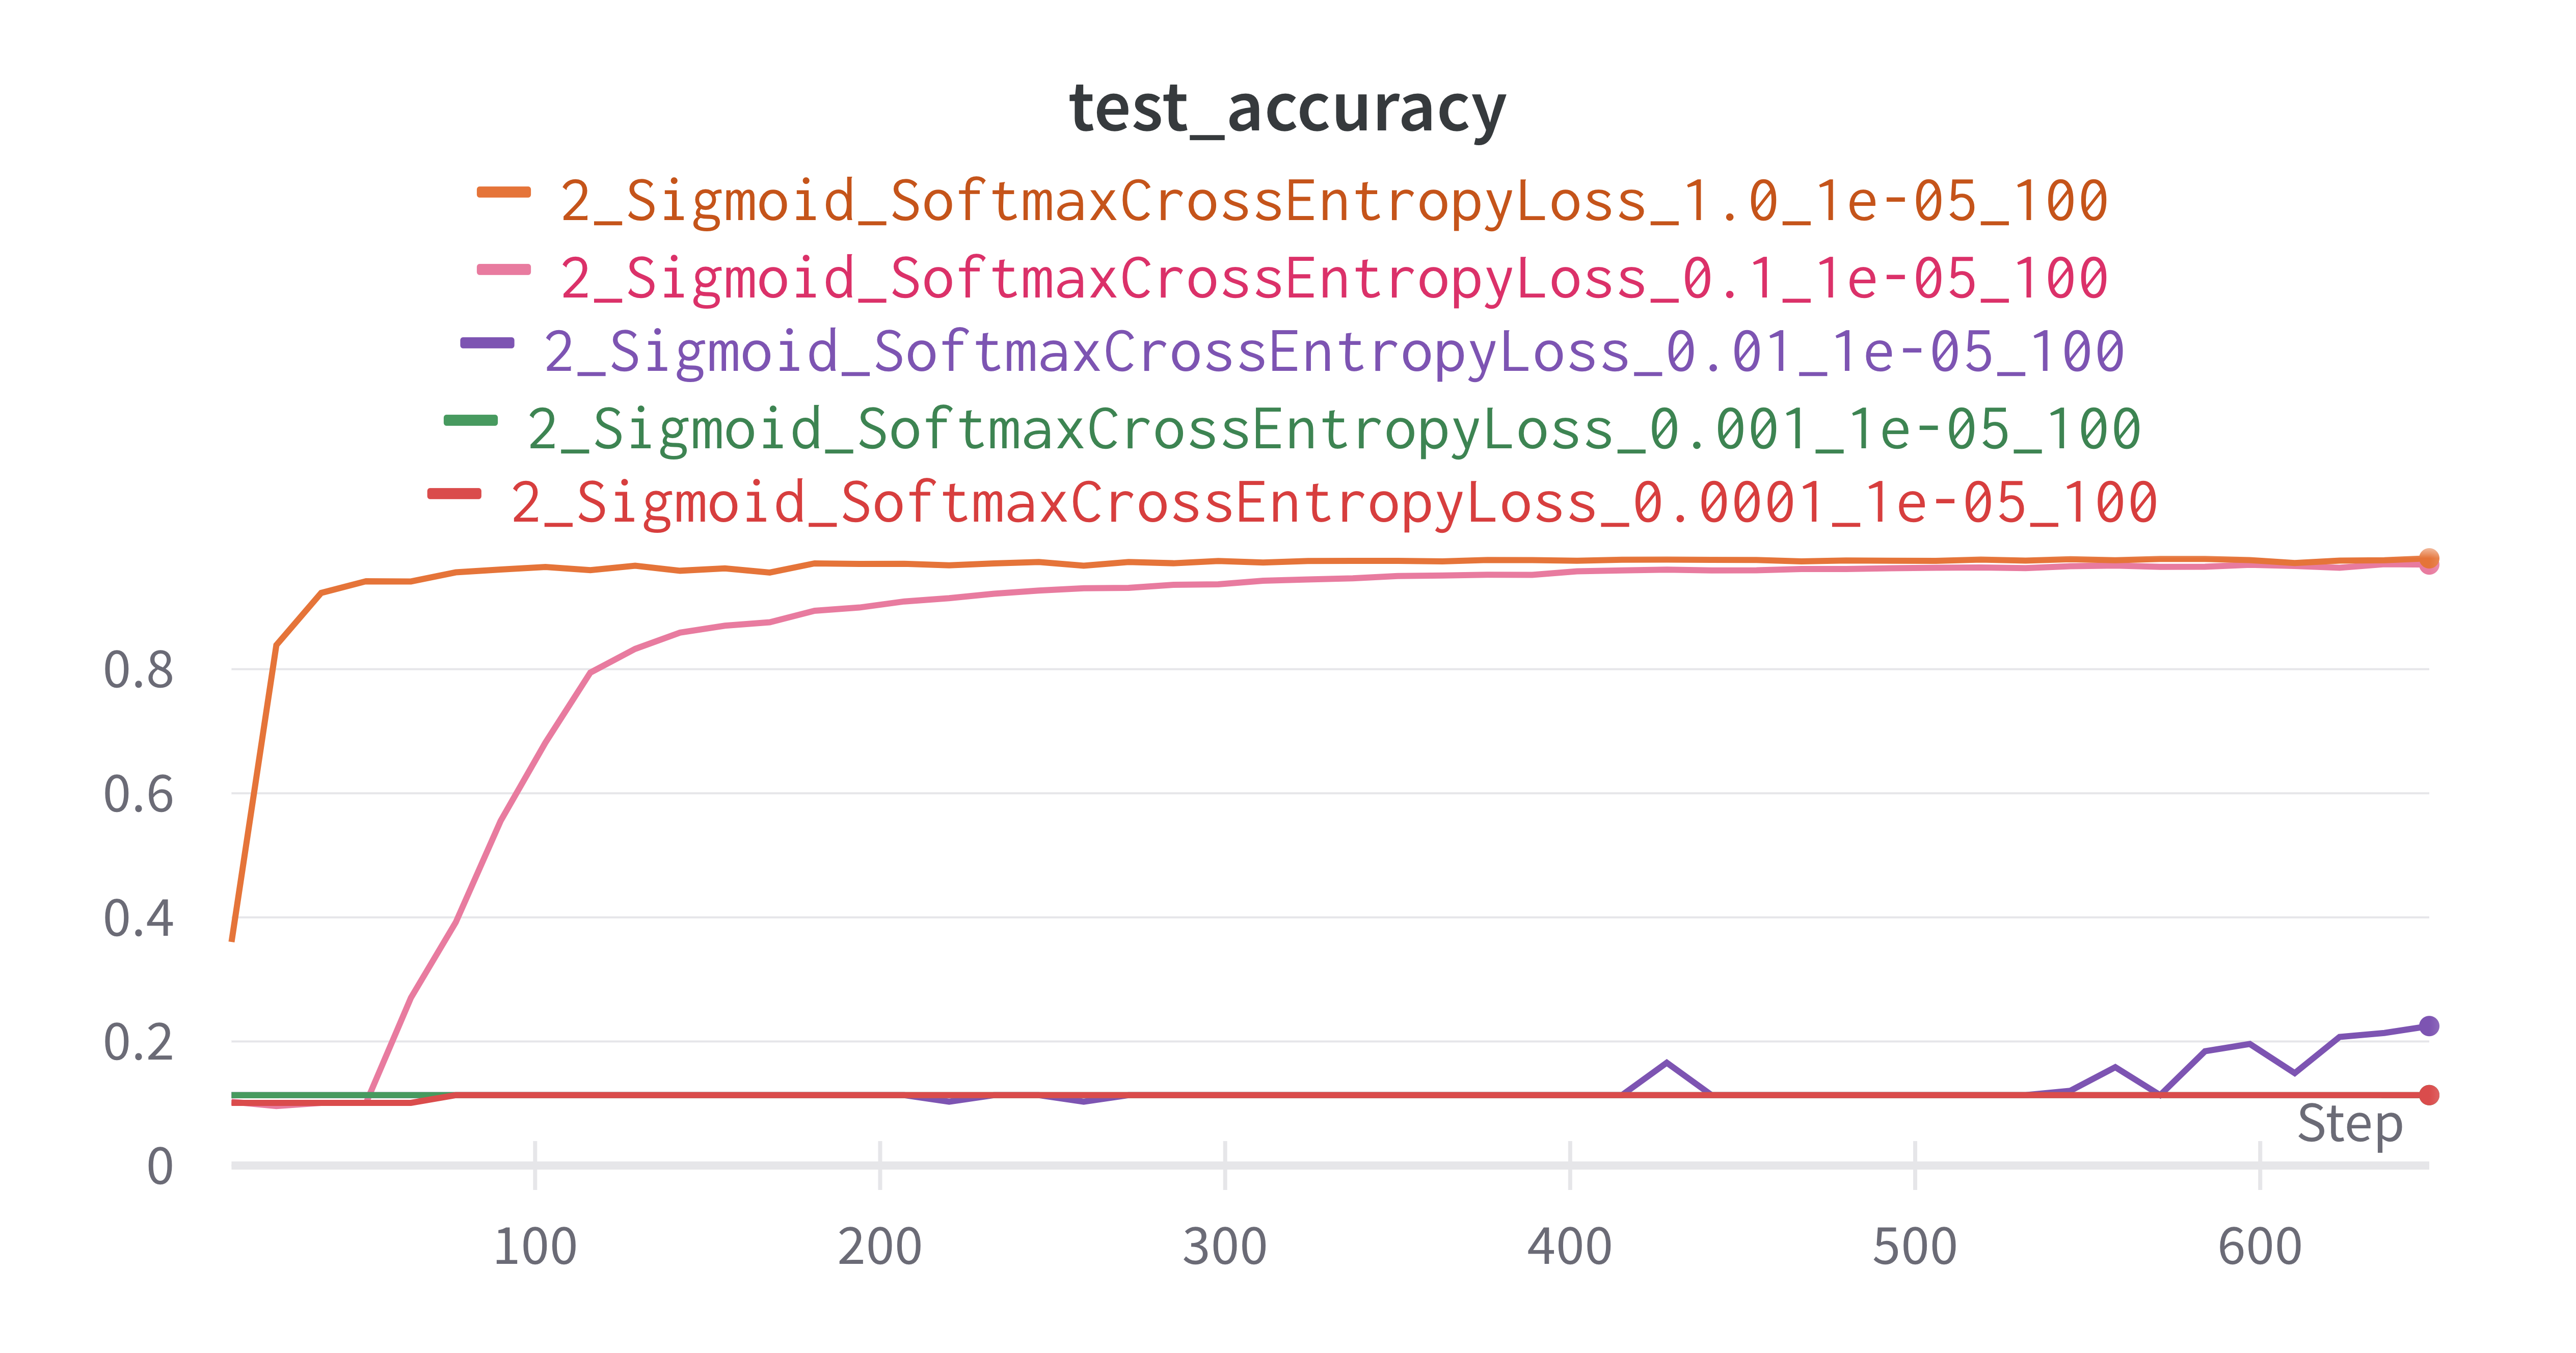
\includegraphics[width=1\textwidth]{../pics/学习率_2_Sigmoid_Softmax_test_acc.png}
		\caption{2\_Sigmoid\_Softmax 对比 test accuracy}
	\end{subfigure}
	\begin{subfigure}{0.475\textwidth}
		\centering
		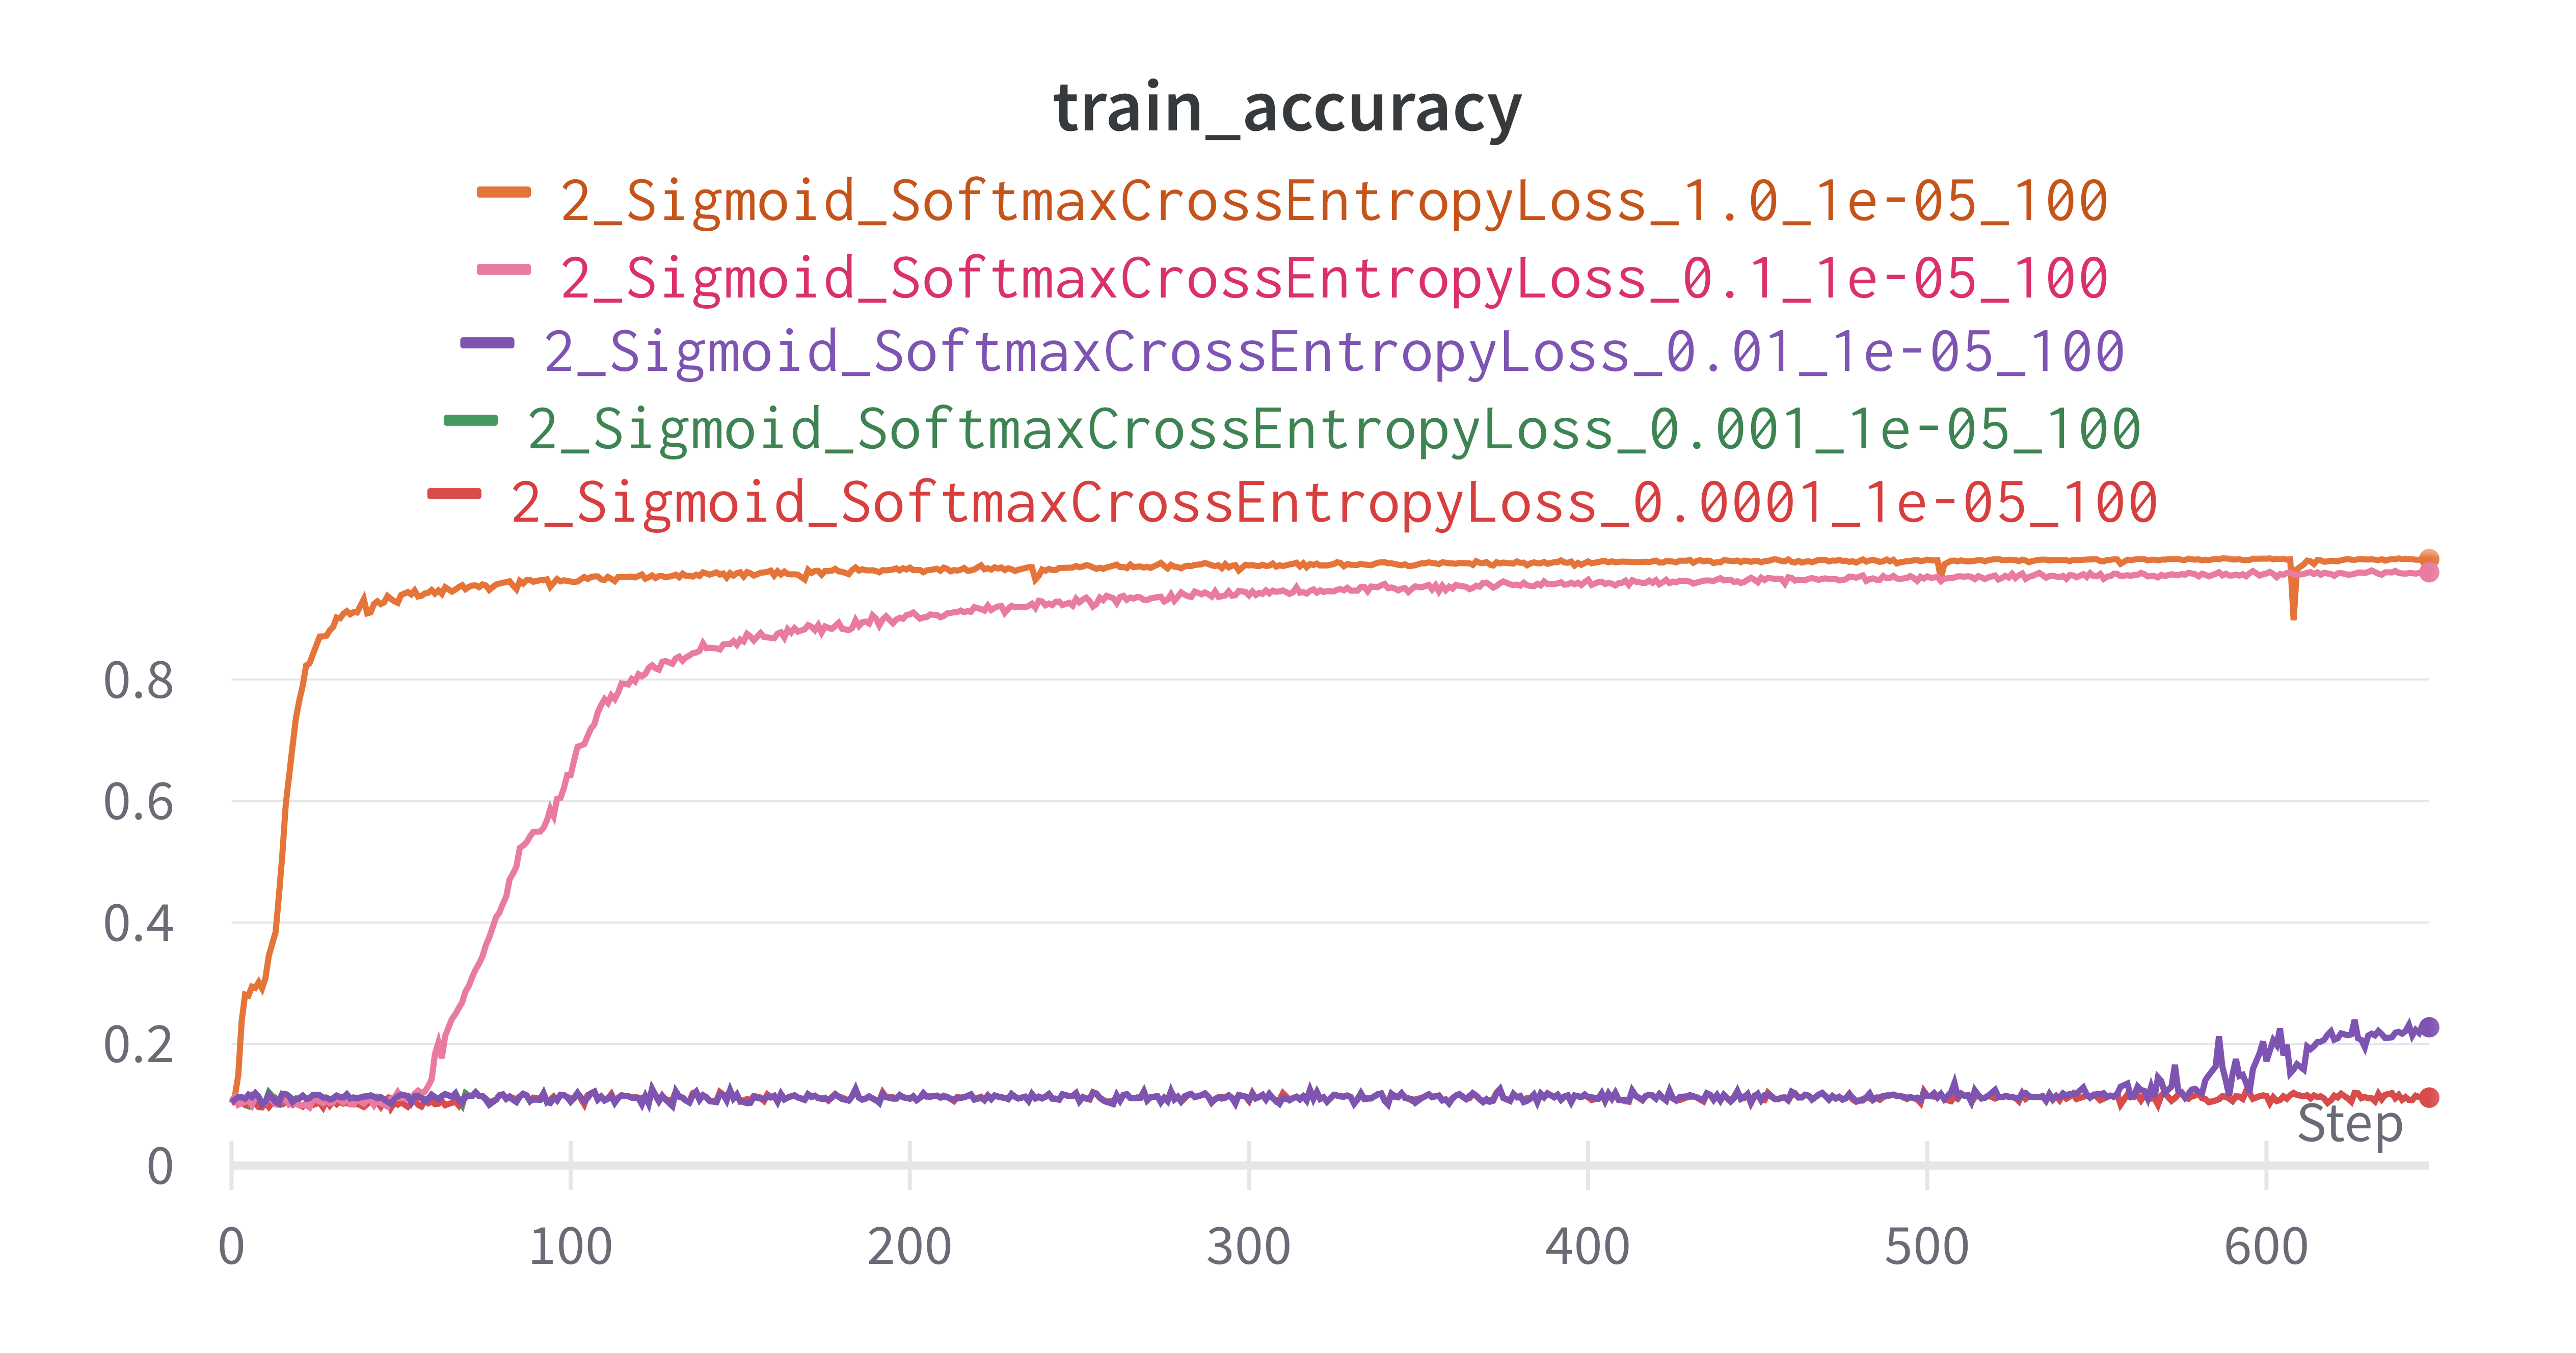
\includegraphics[width=1\textwidth]{../pics/学习率_2_Sigmoid_Softmax_train_acc.png}
		\caption{2\_Sigmoid\_Softmax 对比 train accuracy}
	\end{subfigure}
	\caption{基于 2\_Sigmoid\_Softmax 调节学习率}
	\label{fig:8}
\end{figure}

基于深度学习领域的长期共识,学习率的调整需要基于对于模型本身结构的认知,并没有普适的优秀学习率能够提供普遍优秀的学习效果;譬如大多数模型适用的 1e-2 学习率用于 2\_Sigmoid\_Softmax 和 2\_Sigmoid\_Euclidean 的训练则会完全失败。总体上,对于梯度消失非常严重的双层 Sigmoid 激活函数模型,需要采用较大的学习率,而基于其他激活函数的大多模型能够依靠 1e-2 成功训练。
\\
对于 1\_Sigmoid\_EuclideanLoss 而言可以发现,学习率低于 1e-2 后,随着学习率的减小模型在测试集上的表现会显著降低。观察训练过程的准确率曲线可以发现,随着学习率的增大,参数更新的幅度大幅增大,模型的收敛速度也会变快;然而,模型的表现会出现较大的变动,这在学习率为 1 与 1e-1 的对比上体现的尤为明显。直观上讲,过高的 learning rate 会导致训练很不稳定,同时模型将在多个局部最优值之间反复跳跃。可以猜测,大于 1e-1 后,更大的学习率可能会导致模型难以接近最优的收敛解,最终模型在测试集上的表现也会降低;而较小的学习率却会导致收敛速度过慢以至于在设定的 epoch 次数上训练难以达到最优解,最终在有限的训练成本下,模型在测试集上的表现也会降低。
\\最后,由于本次实验任务较为简单等缘故,实验并没有出现过拟合的情况,而在学习率较低时体现出欠拟合的情况。

\subsection{消减率影响}

保留除了学习率和 weight decay 之外的基础实验参数设定,模型选取 2\_Gelu\_HingeLoss 以 1e-2 为学习率(图 \ref{fig:9})与 2\_Sigmoid\_Softmax 以 1 为学习率(图 \ref{fig:10}),消减率选取为 \{1e-4, 1e-3, 1e-2, 1e-1, 1\},展开消减率对比实验。

\begin{figure}[htbp]
	\centering
	\begin{subfigure}{0.475\textwidth}
		\centering
		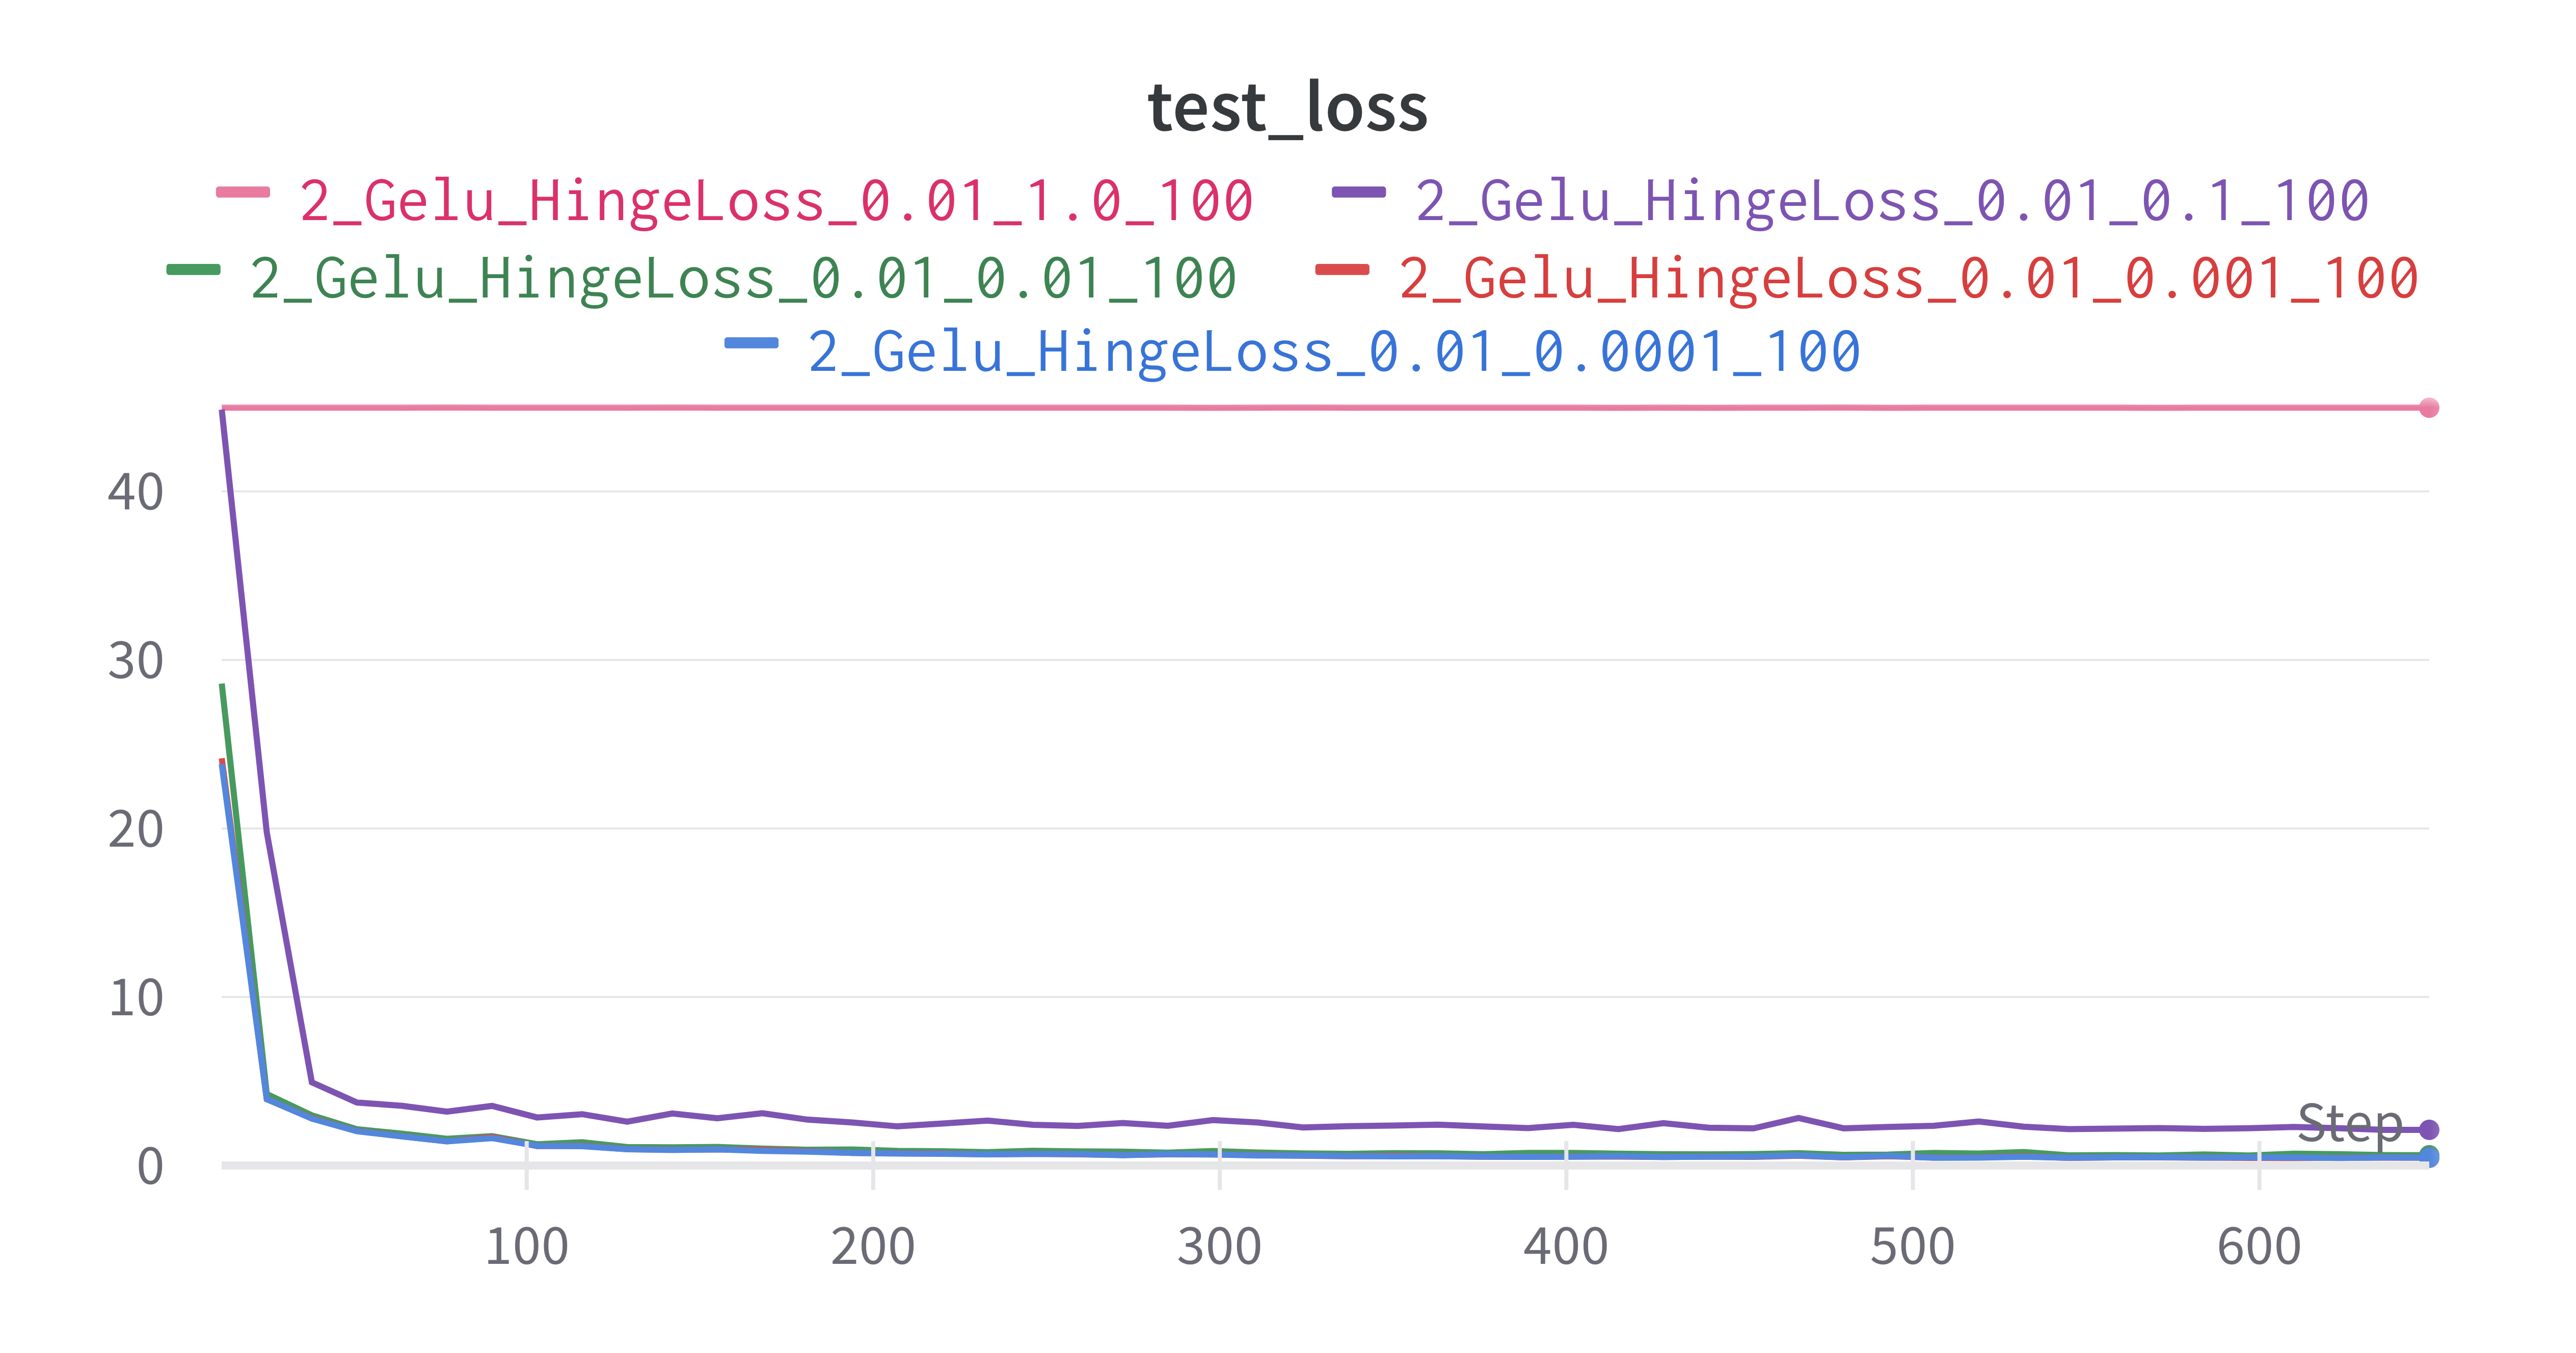
\includegraphics[width=1\textwidth]{../pics/消减率_2_Gelu_HingeLoss_test_loss.png}
		\caption{2\_Gelu\_HingeLoss 对比 test loss}
	\end{subfigure}
	\begin{subfigure}{0.475\textwidth}
		\centering
		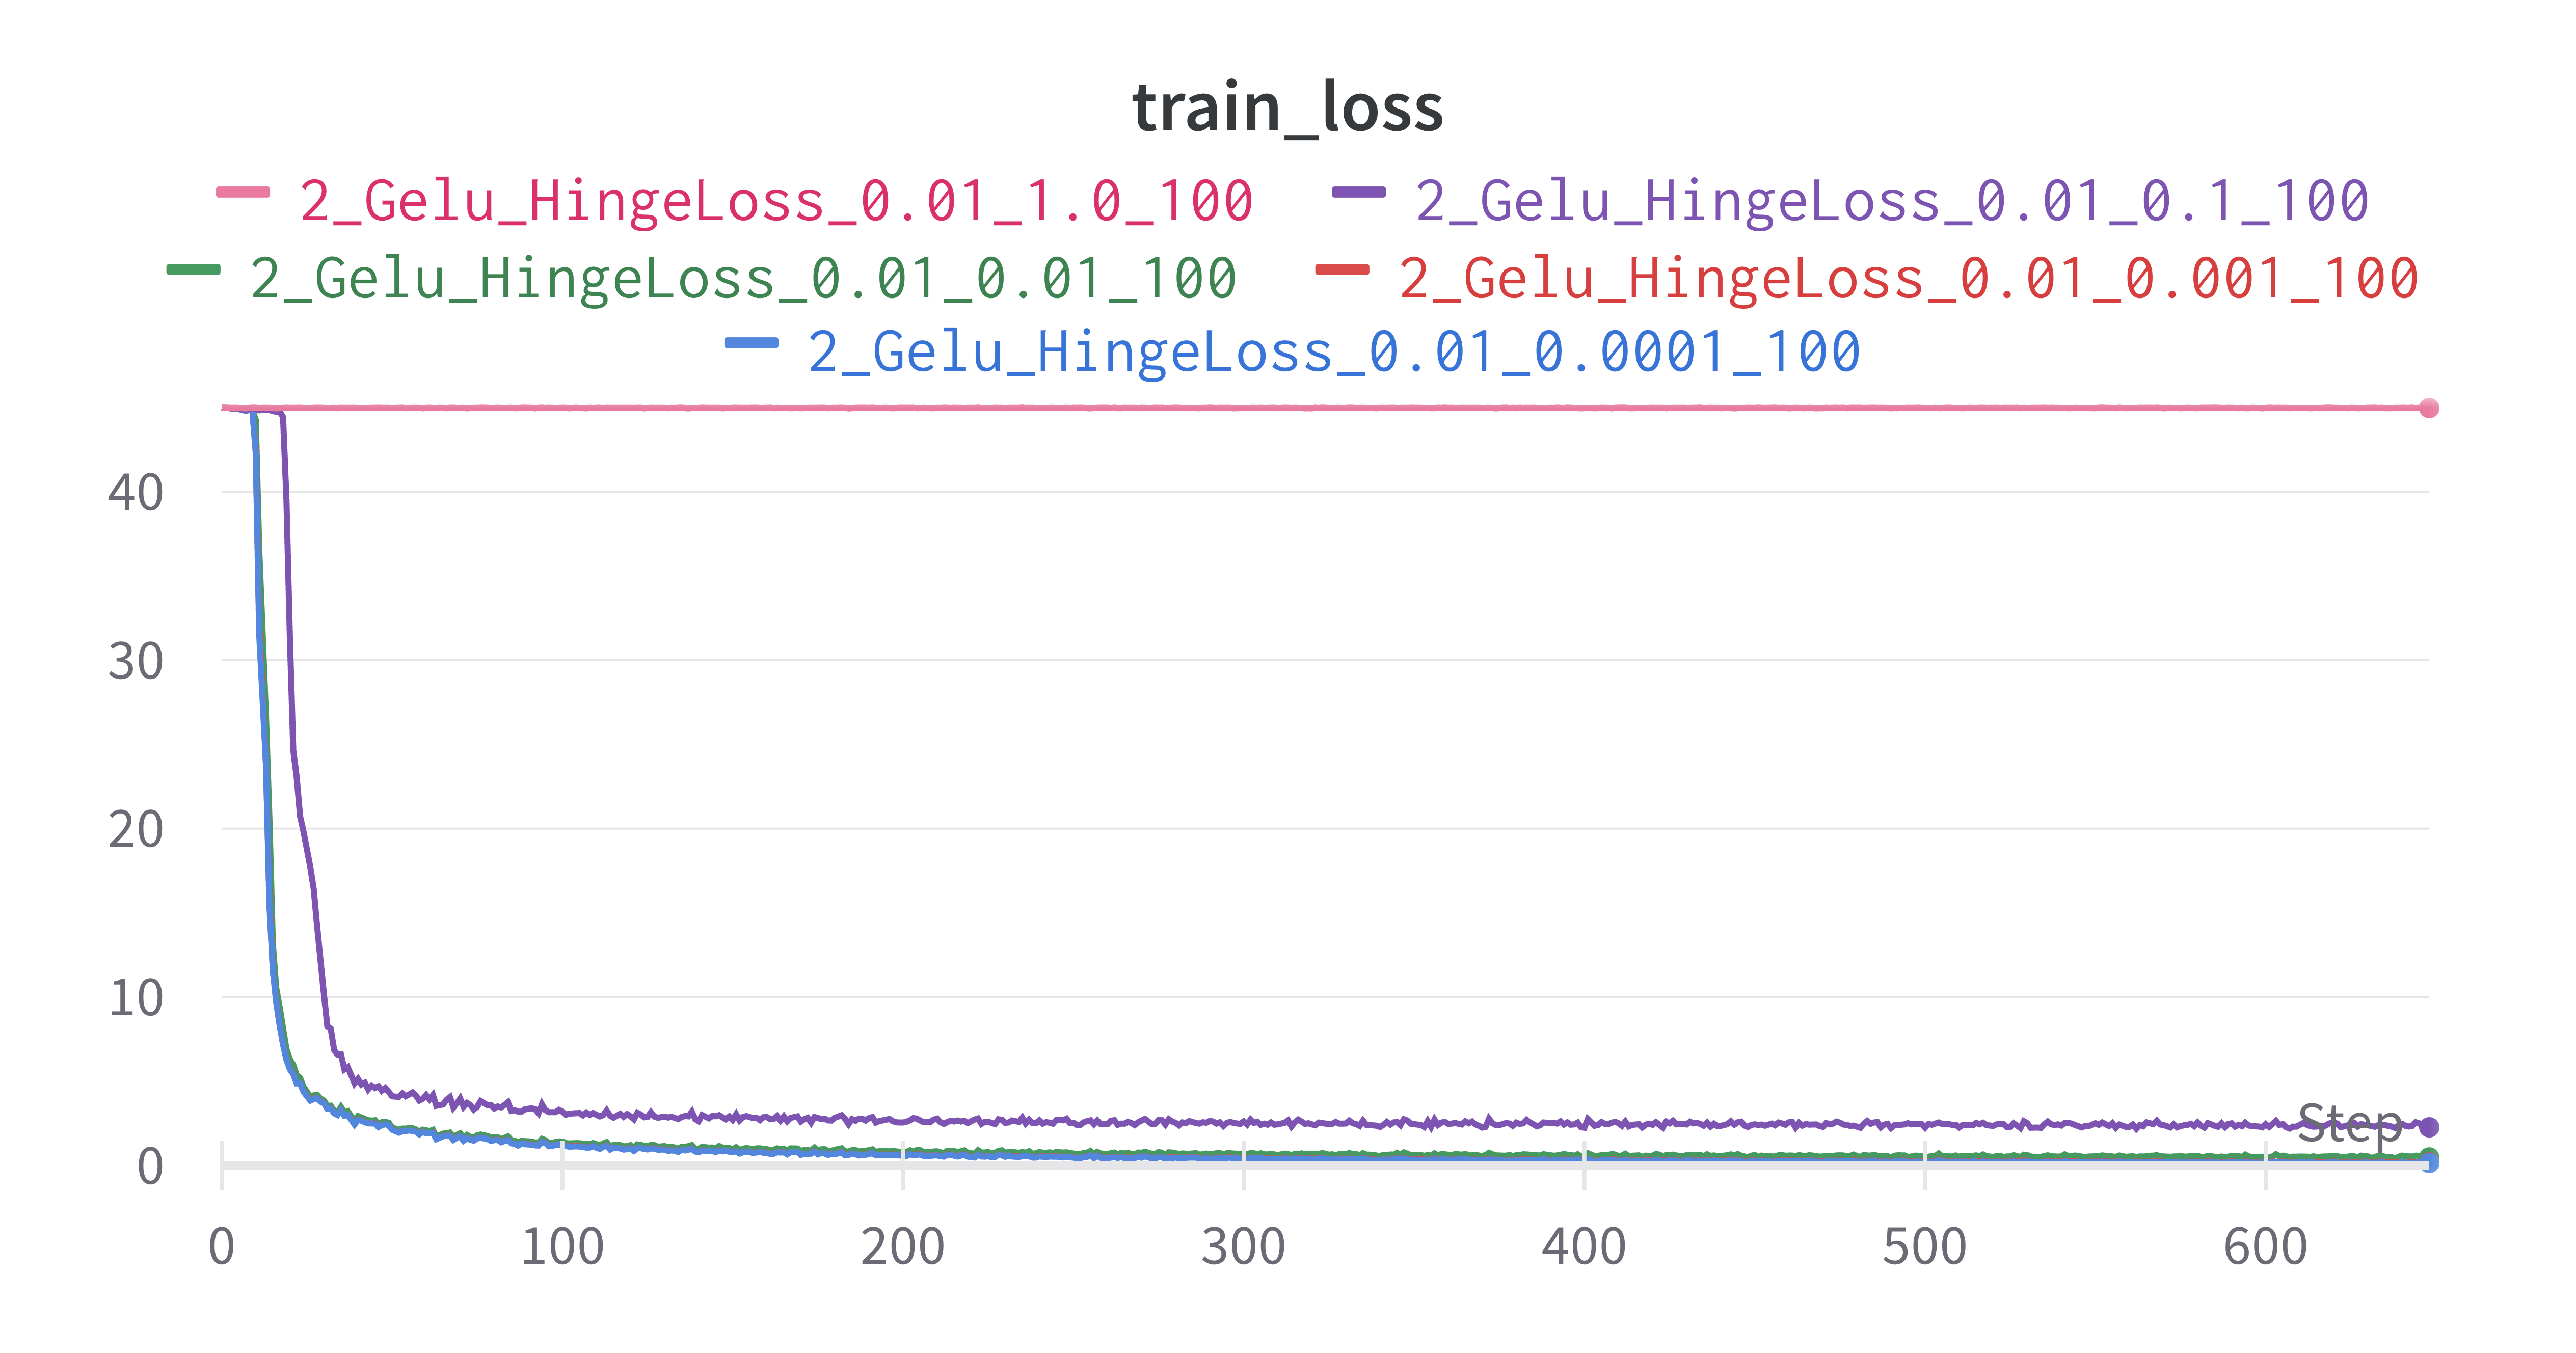
\includegraphics[width=1\textwidth]{../pics/消减率_2_Gelu_HingeLoss_train_loss.png}
		\caption{2\_Gelu\_HingeLoss 对比 train loss}
	\end{subfigure}
	\begin{subfigure}{0.475\textwidth}
		\centering
		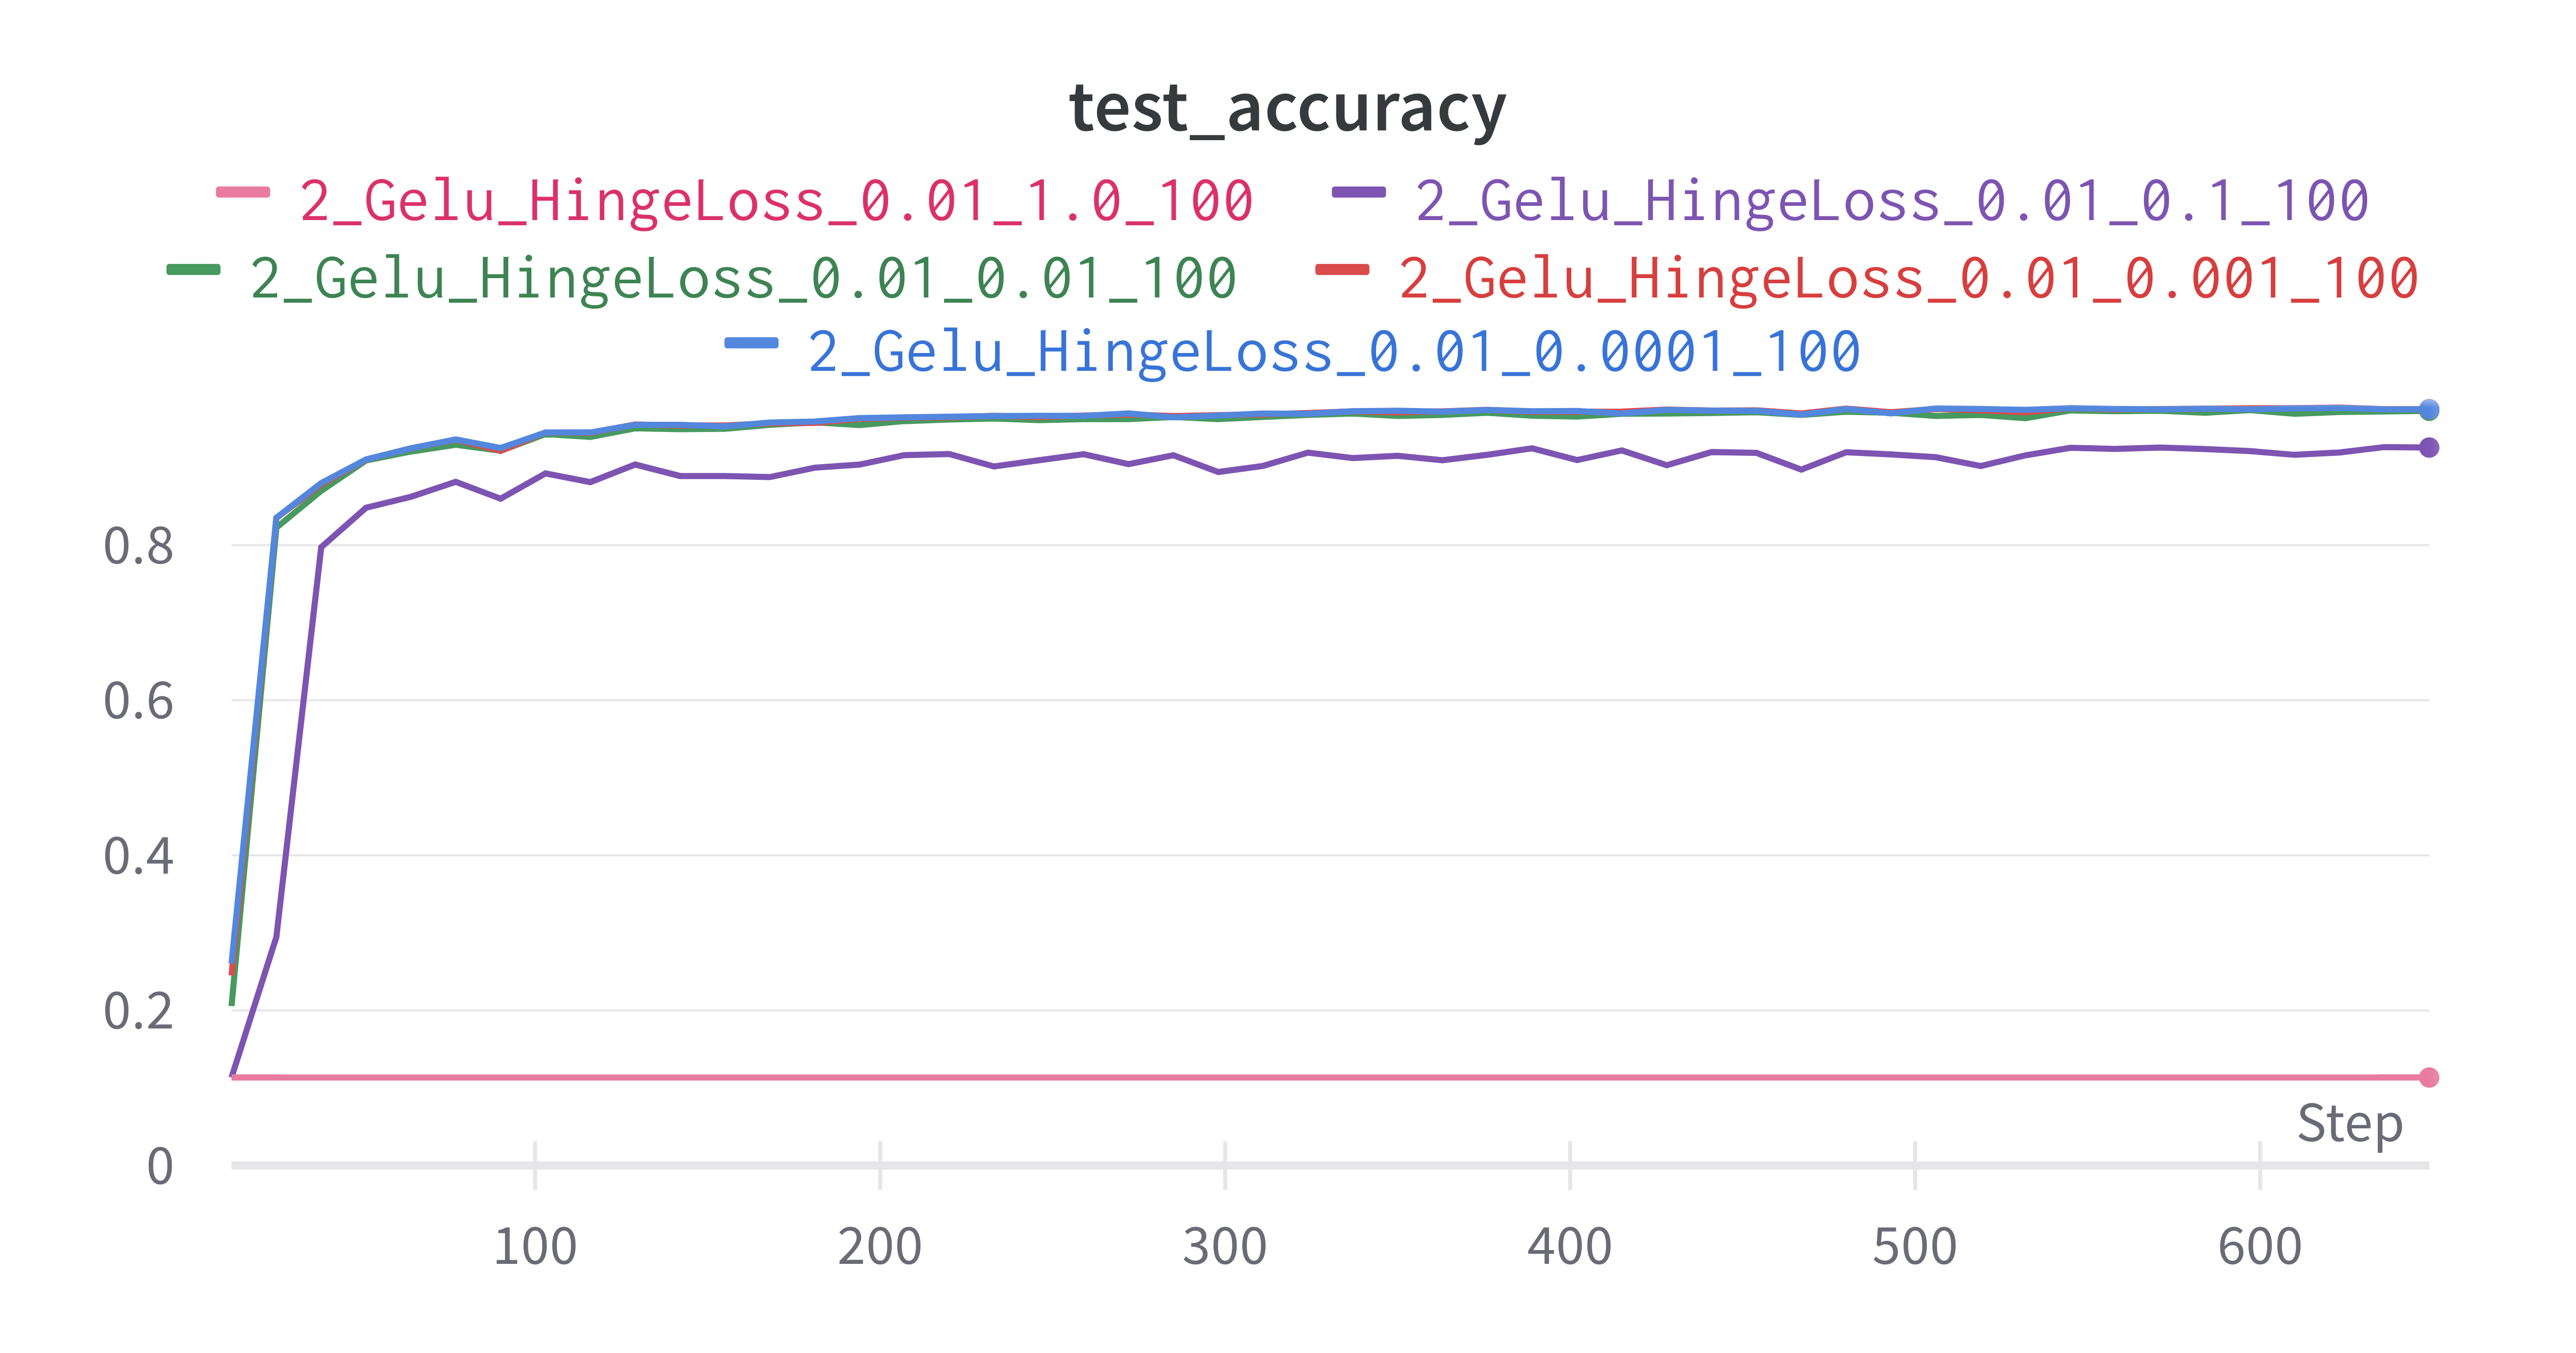
\includegraphics[width=1\textwidth]{../pics/消减率_2_Gelu_HingeLoss_test_acc.png}
		\caption{2\_Gelu\_HingeLoss 对比 test accuracy}
	\end{subfigure}
	\begin{subfigure}{0.475\textwidth}
		\centering
		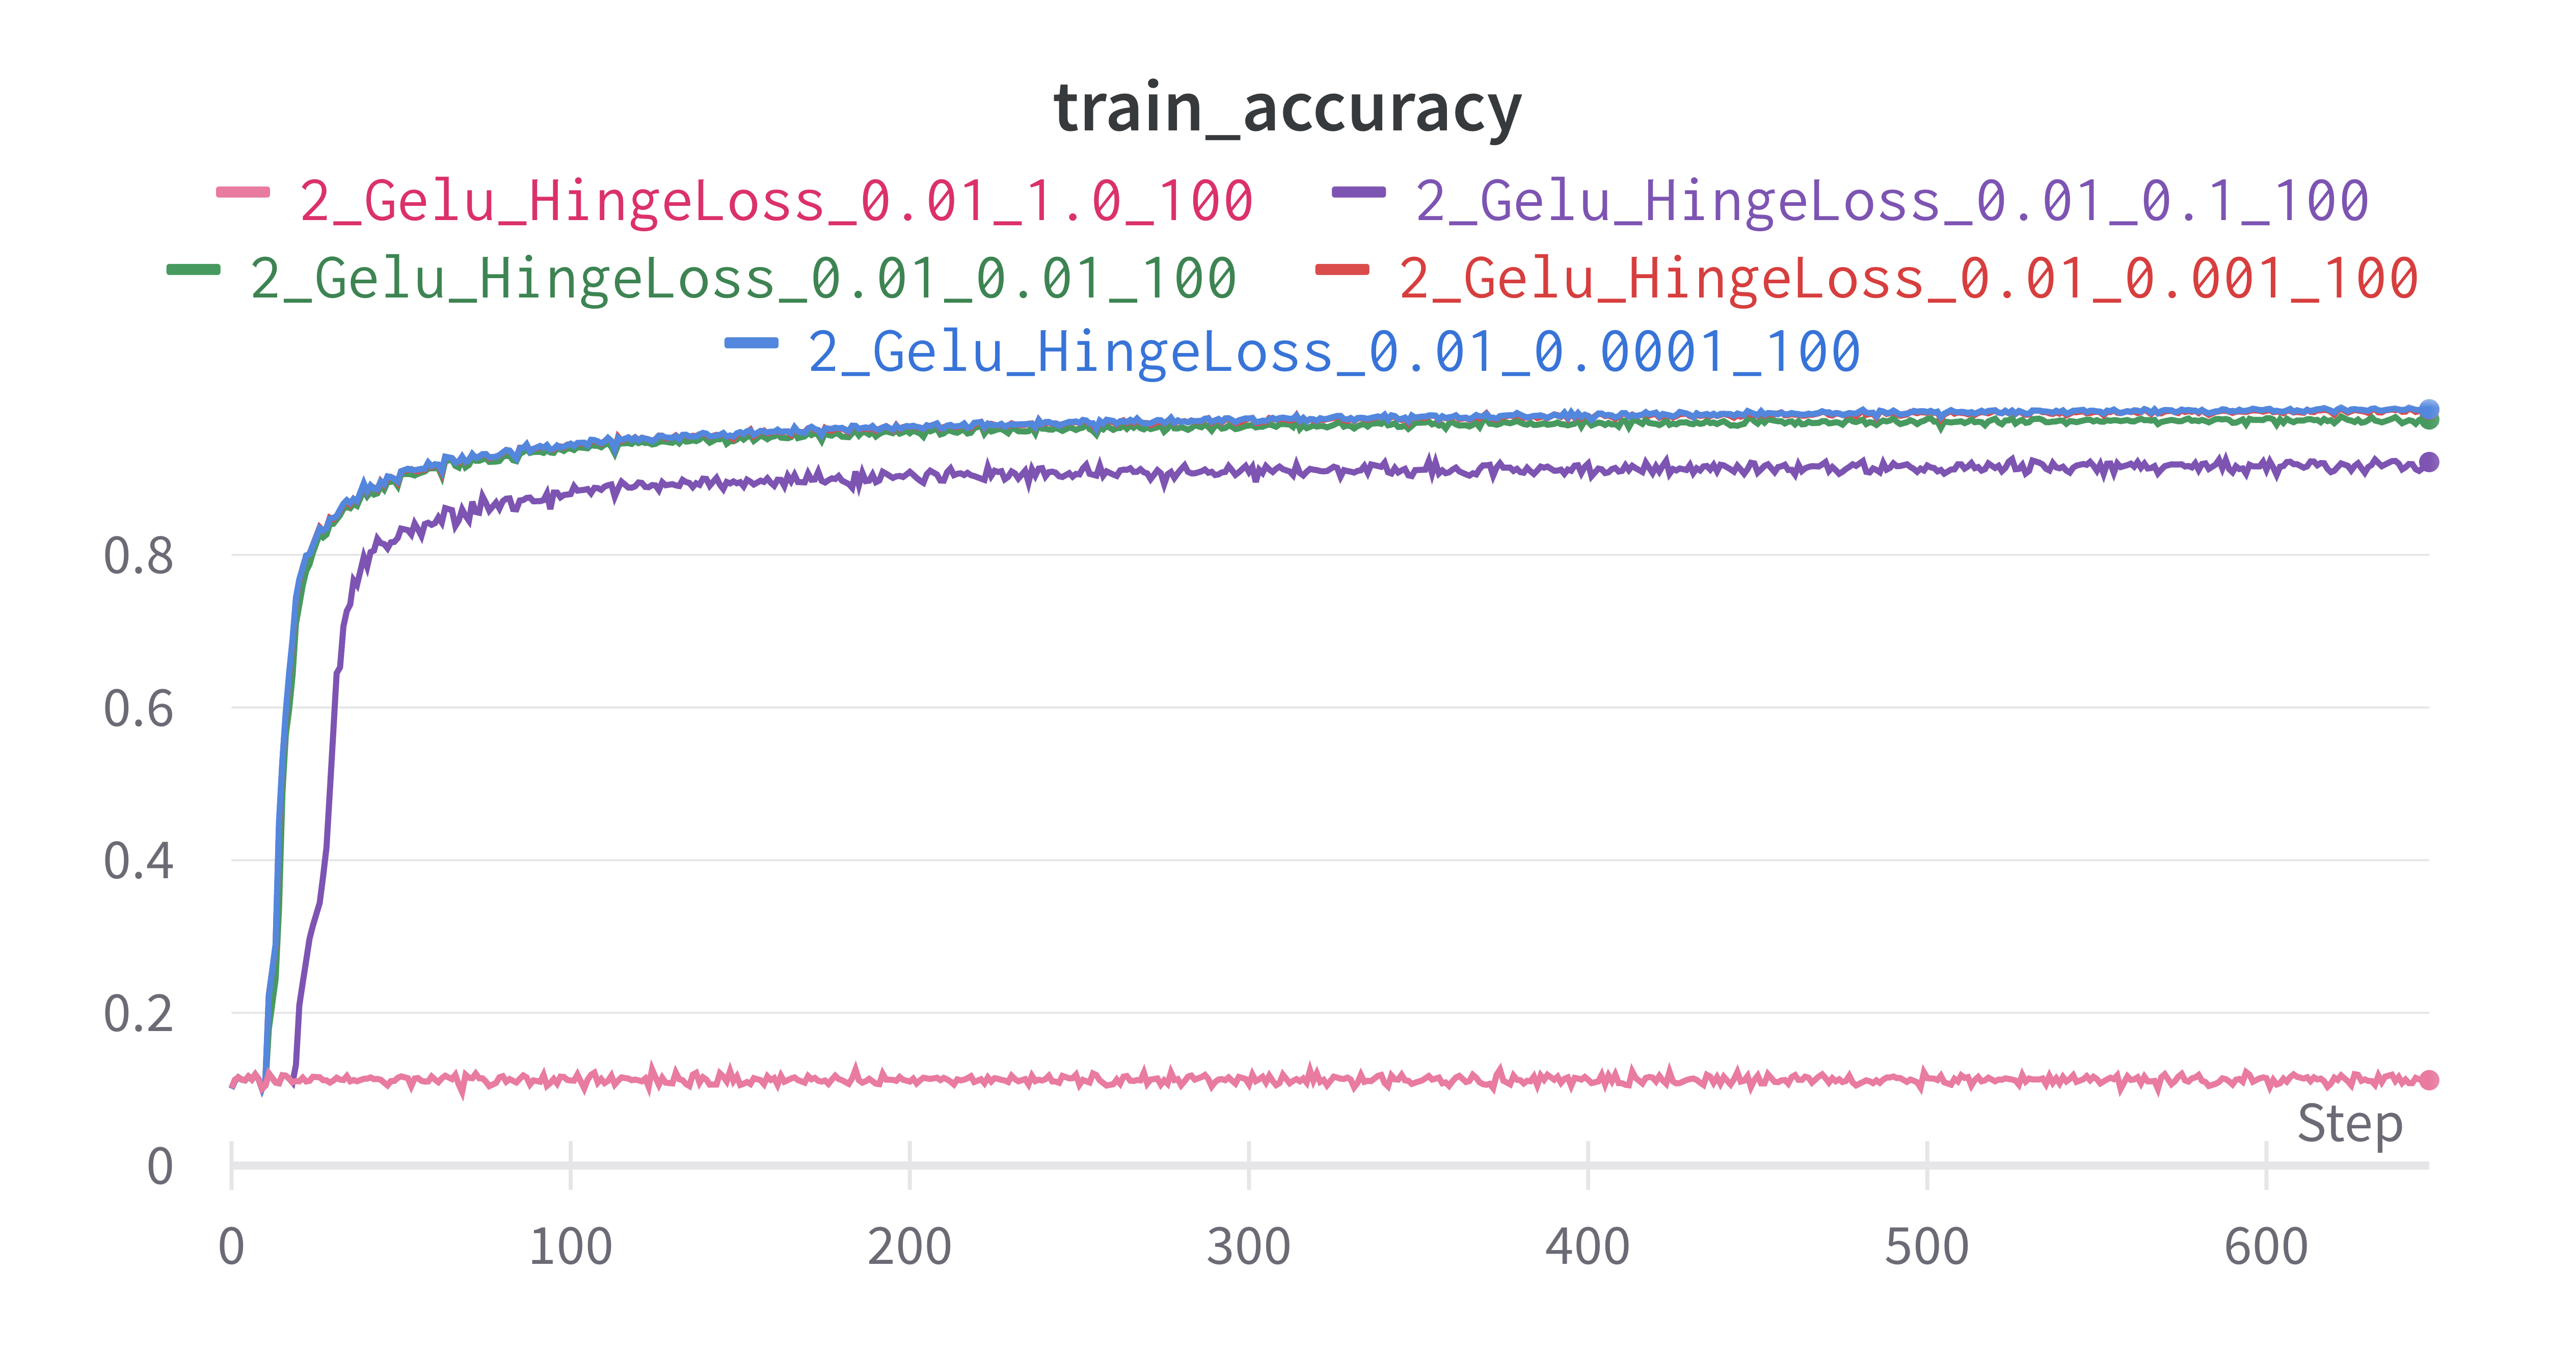
\includegraphics[width=1\textwidth]{../pics/消减率_2_Gelu_HingeLoss_train_acc.png}
		\caption{2\_Gelu\_HingeLoss  对比 train accuracy}
	\end{subfigure}
	\caption{基于 2\_Gelu\_HingeLoss  调节消减率}
	\label{fig:9}
\end{figure}

\begin{figure}[htbp]
	\centering
	\begin{subfigure}{0.475\textwidth}
		\centering
		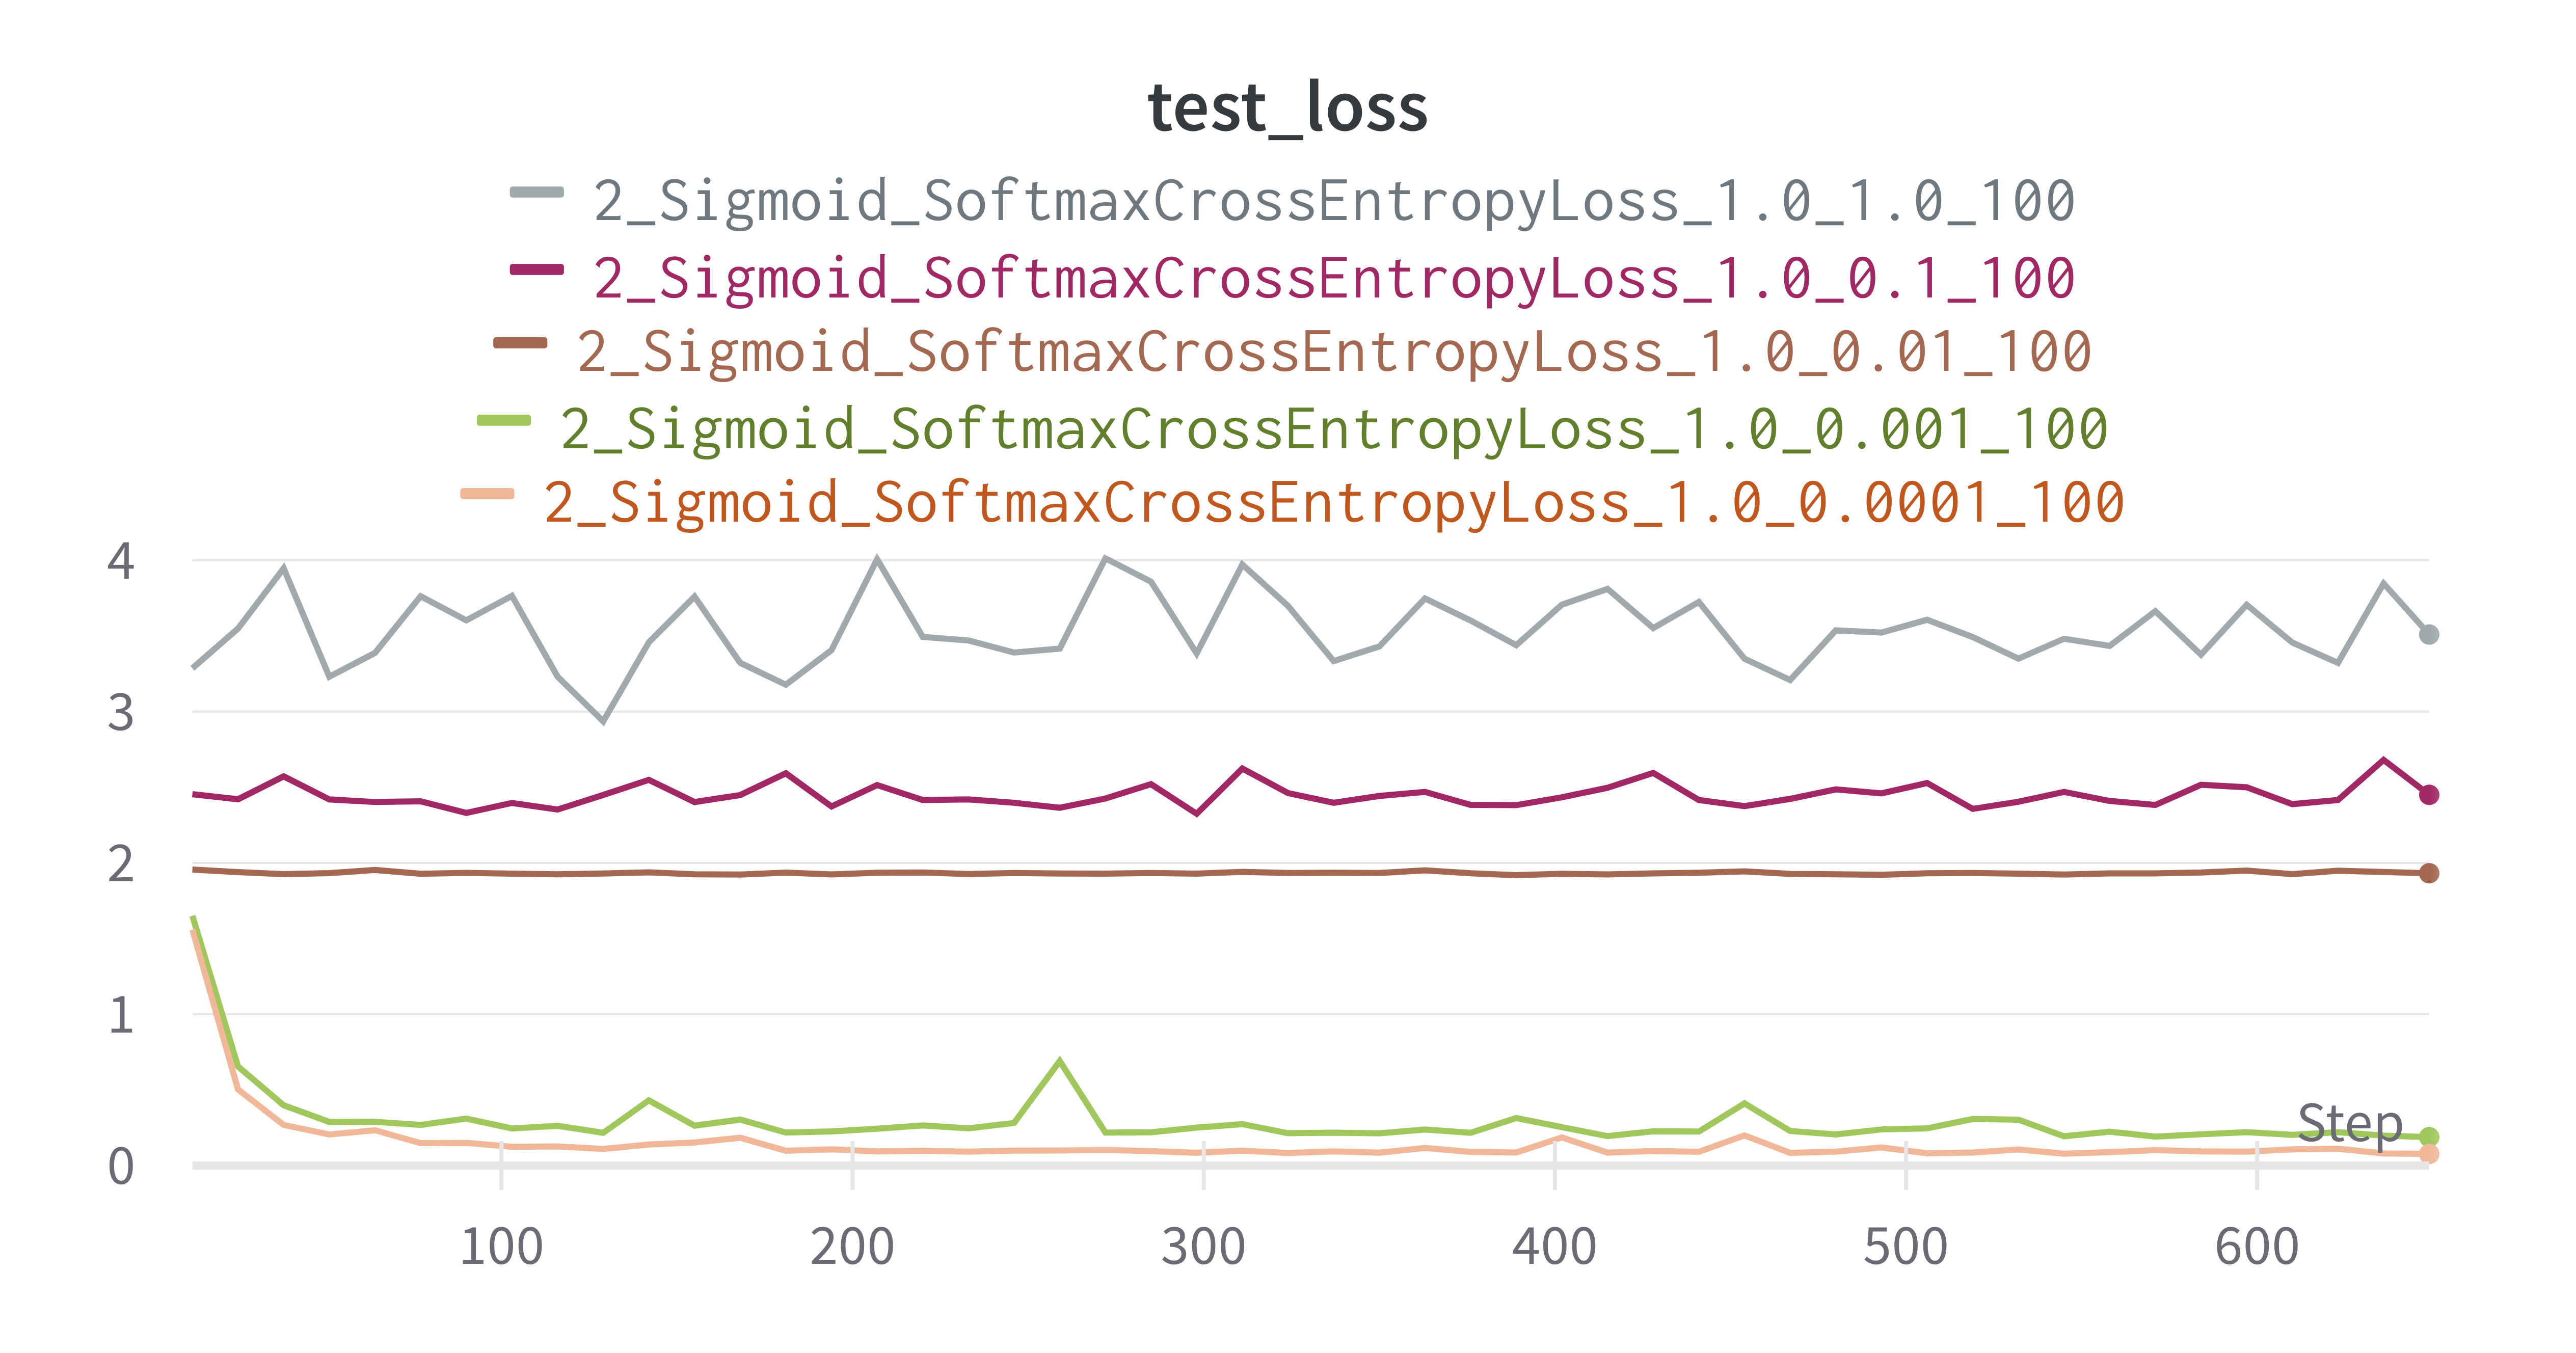
\includegraphics[width=1\textwidth]{../pics/消减率_2_Sigmoid_SoftmaxCross_test_loss.png}
		\caption{2\_Sigmoid\_Softmax 对比 test loss}
	\end{subfigure}
	\begin{subfigure}{0.475\textwidth}
		\centering
		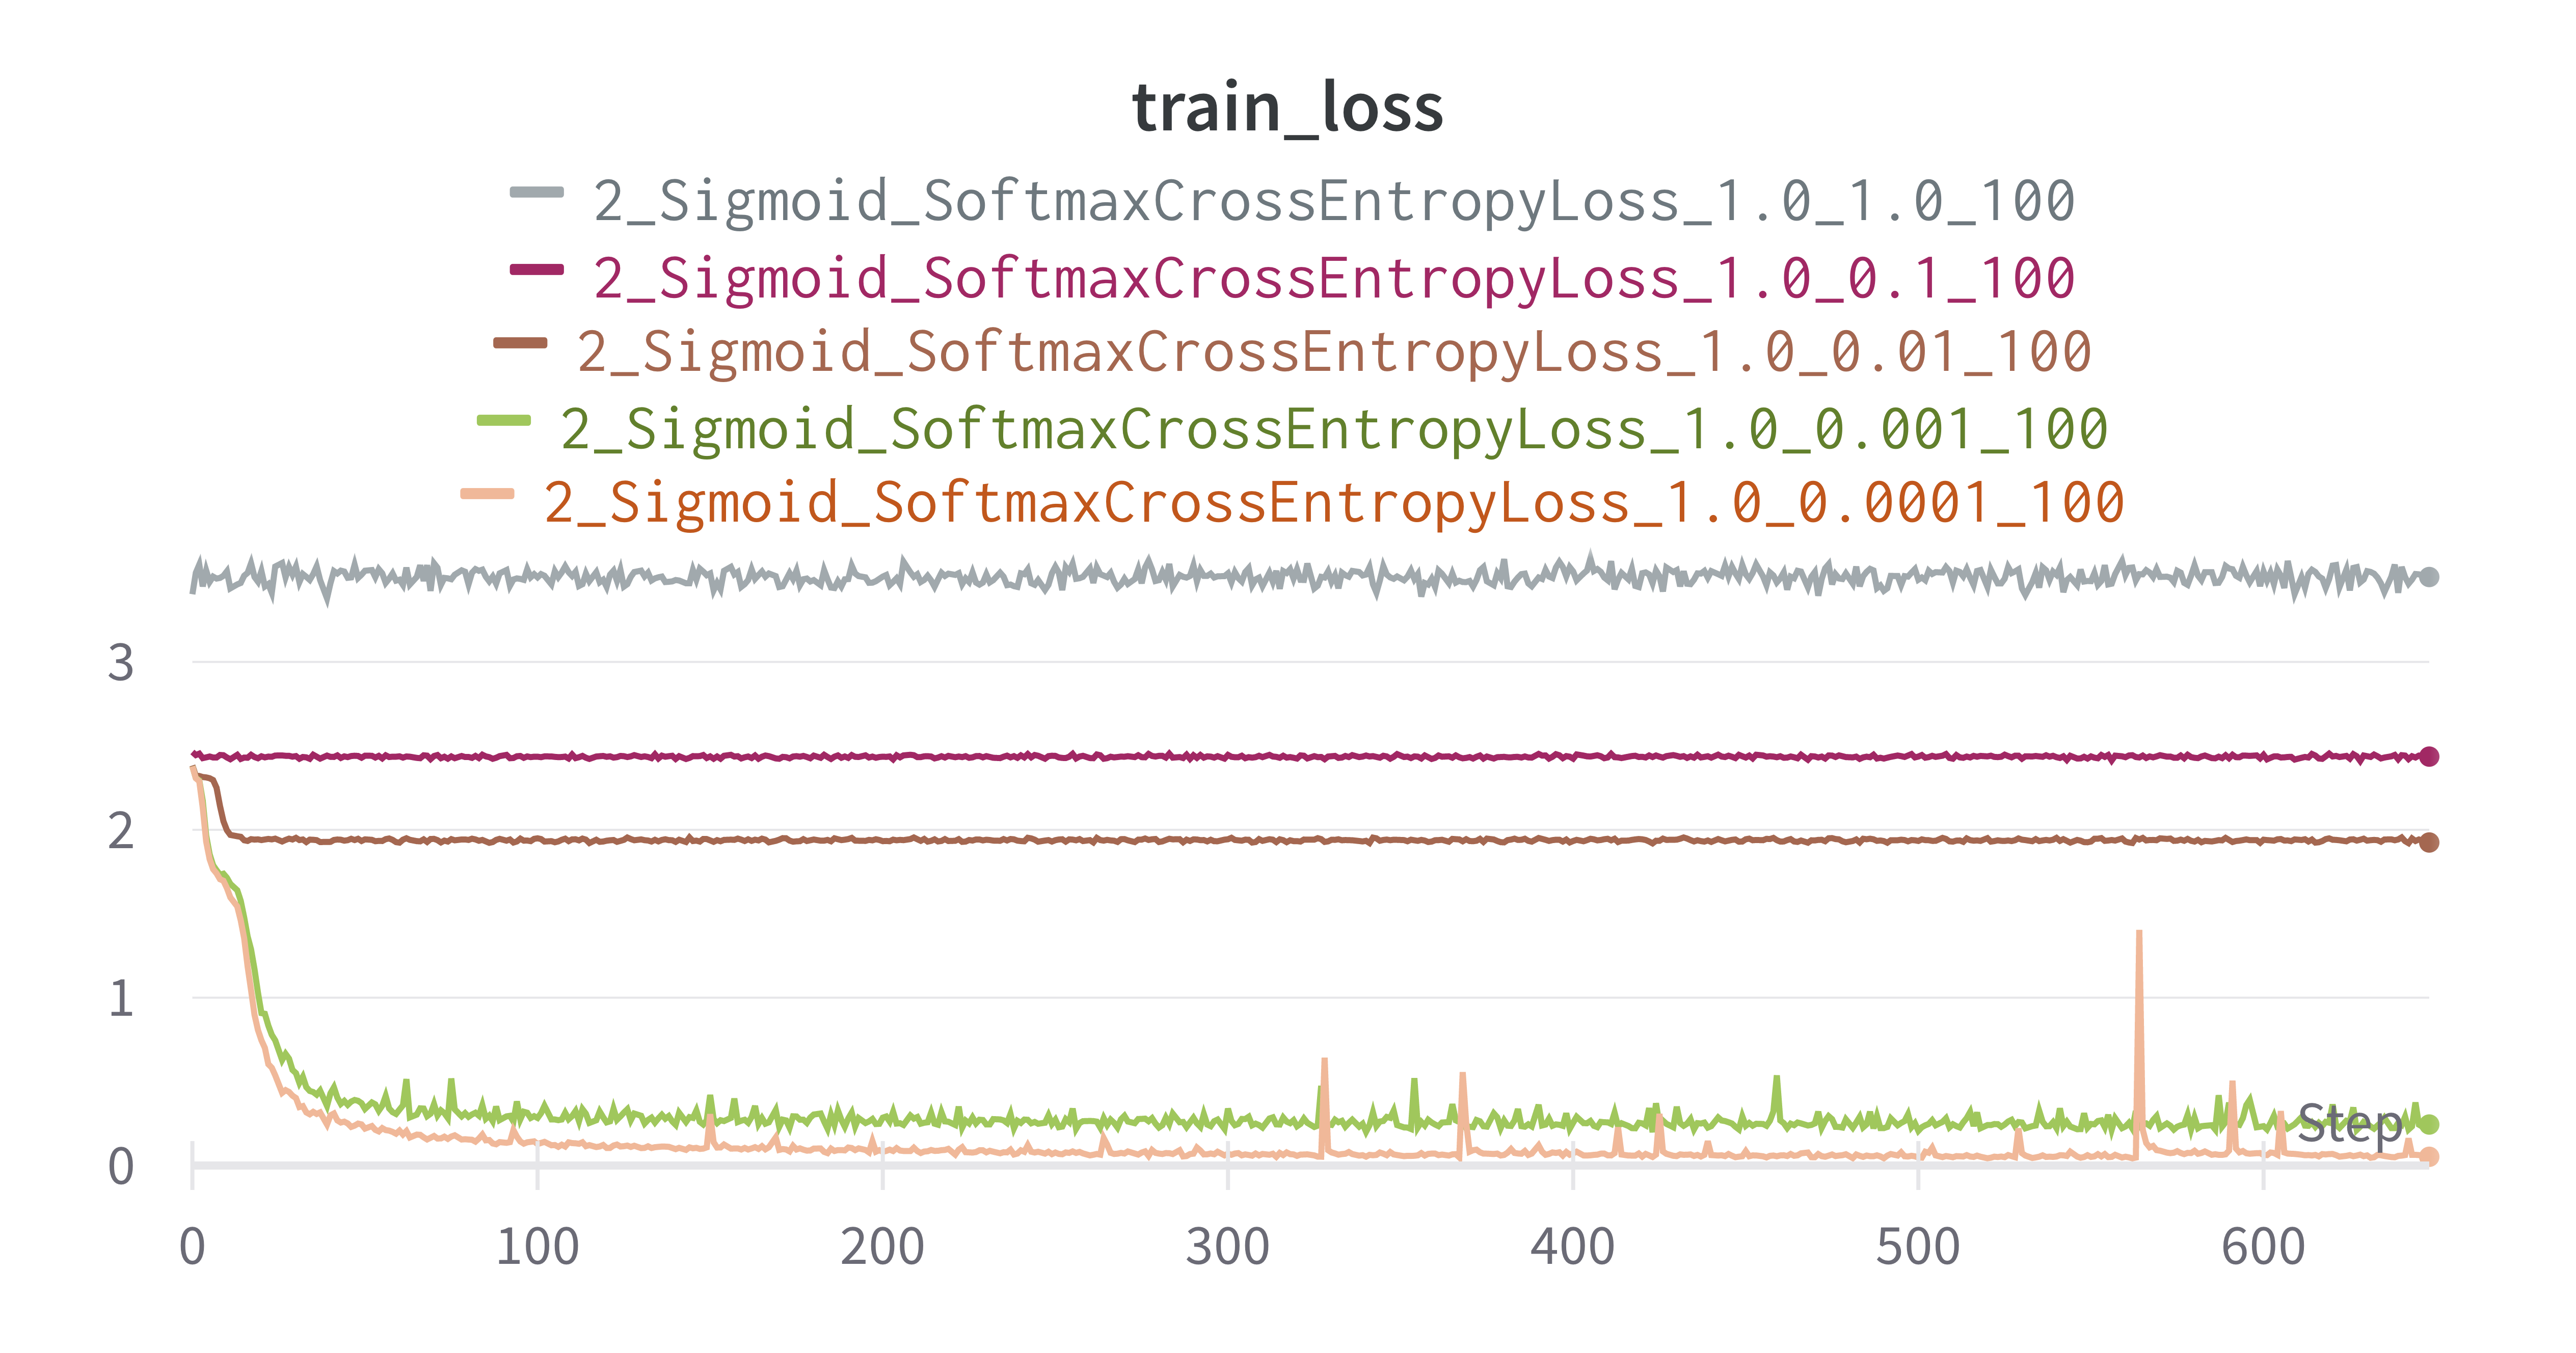
\includegraphics[width=1\textwidth]{../pics/消减率_2_Sigmoid_SoftmaxCross_train_loss.png}
		\caption{2\_Sigmoid\_Softmax 对比 train loss}
	\end{subfigure}
	\begin{subfigure}{0.475\textwidth}
		\centering
		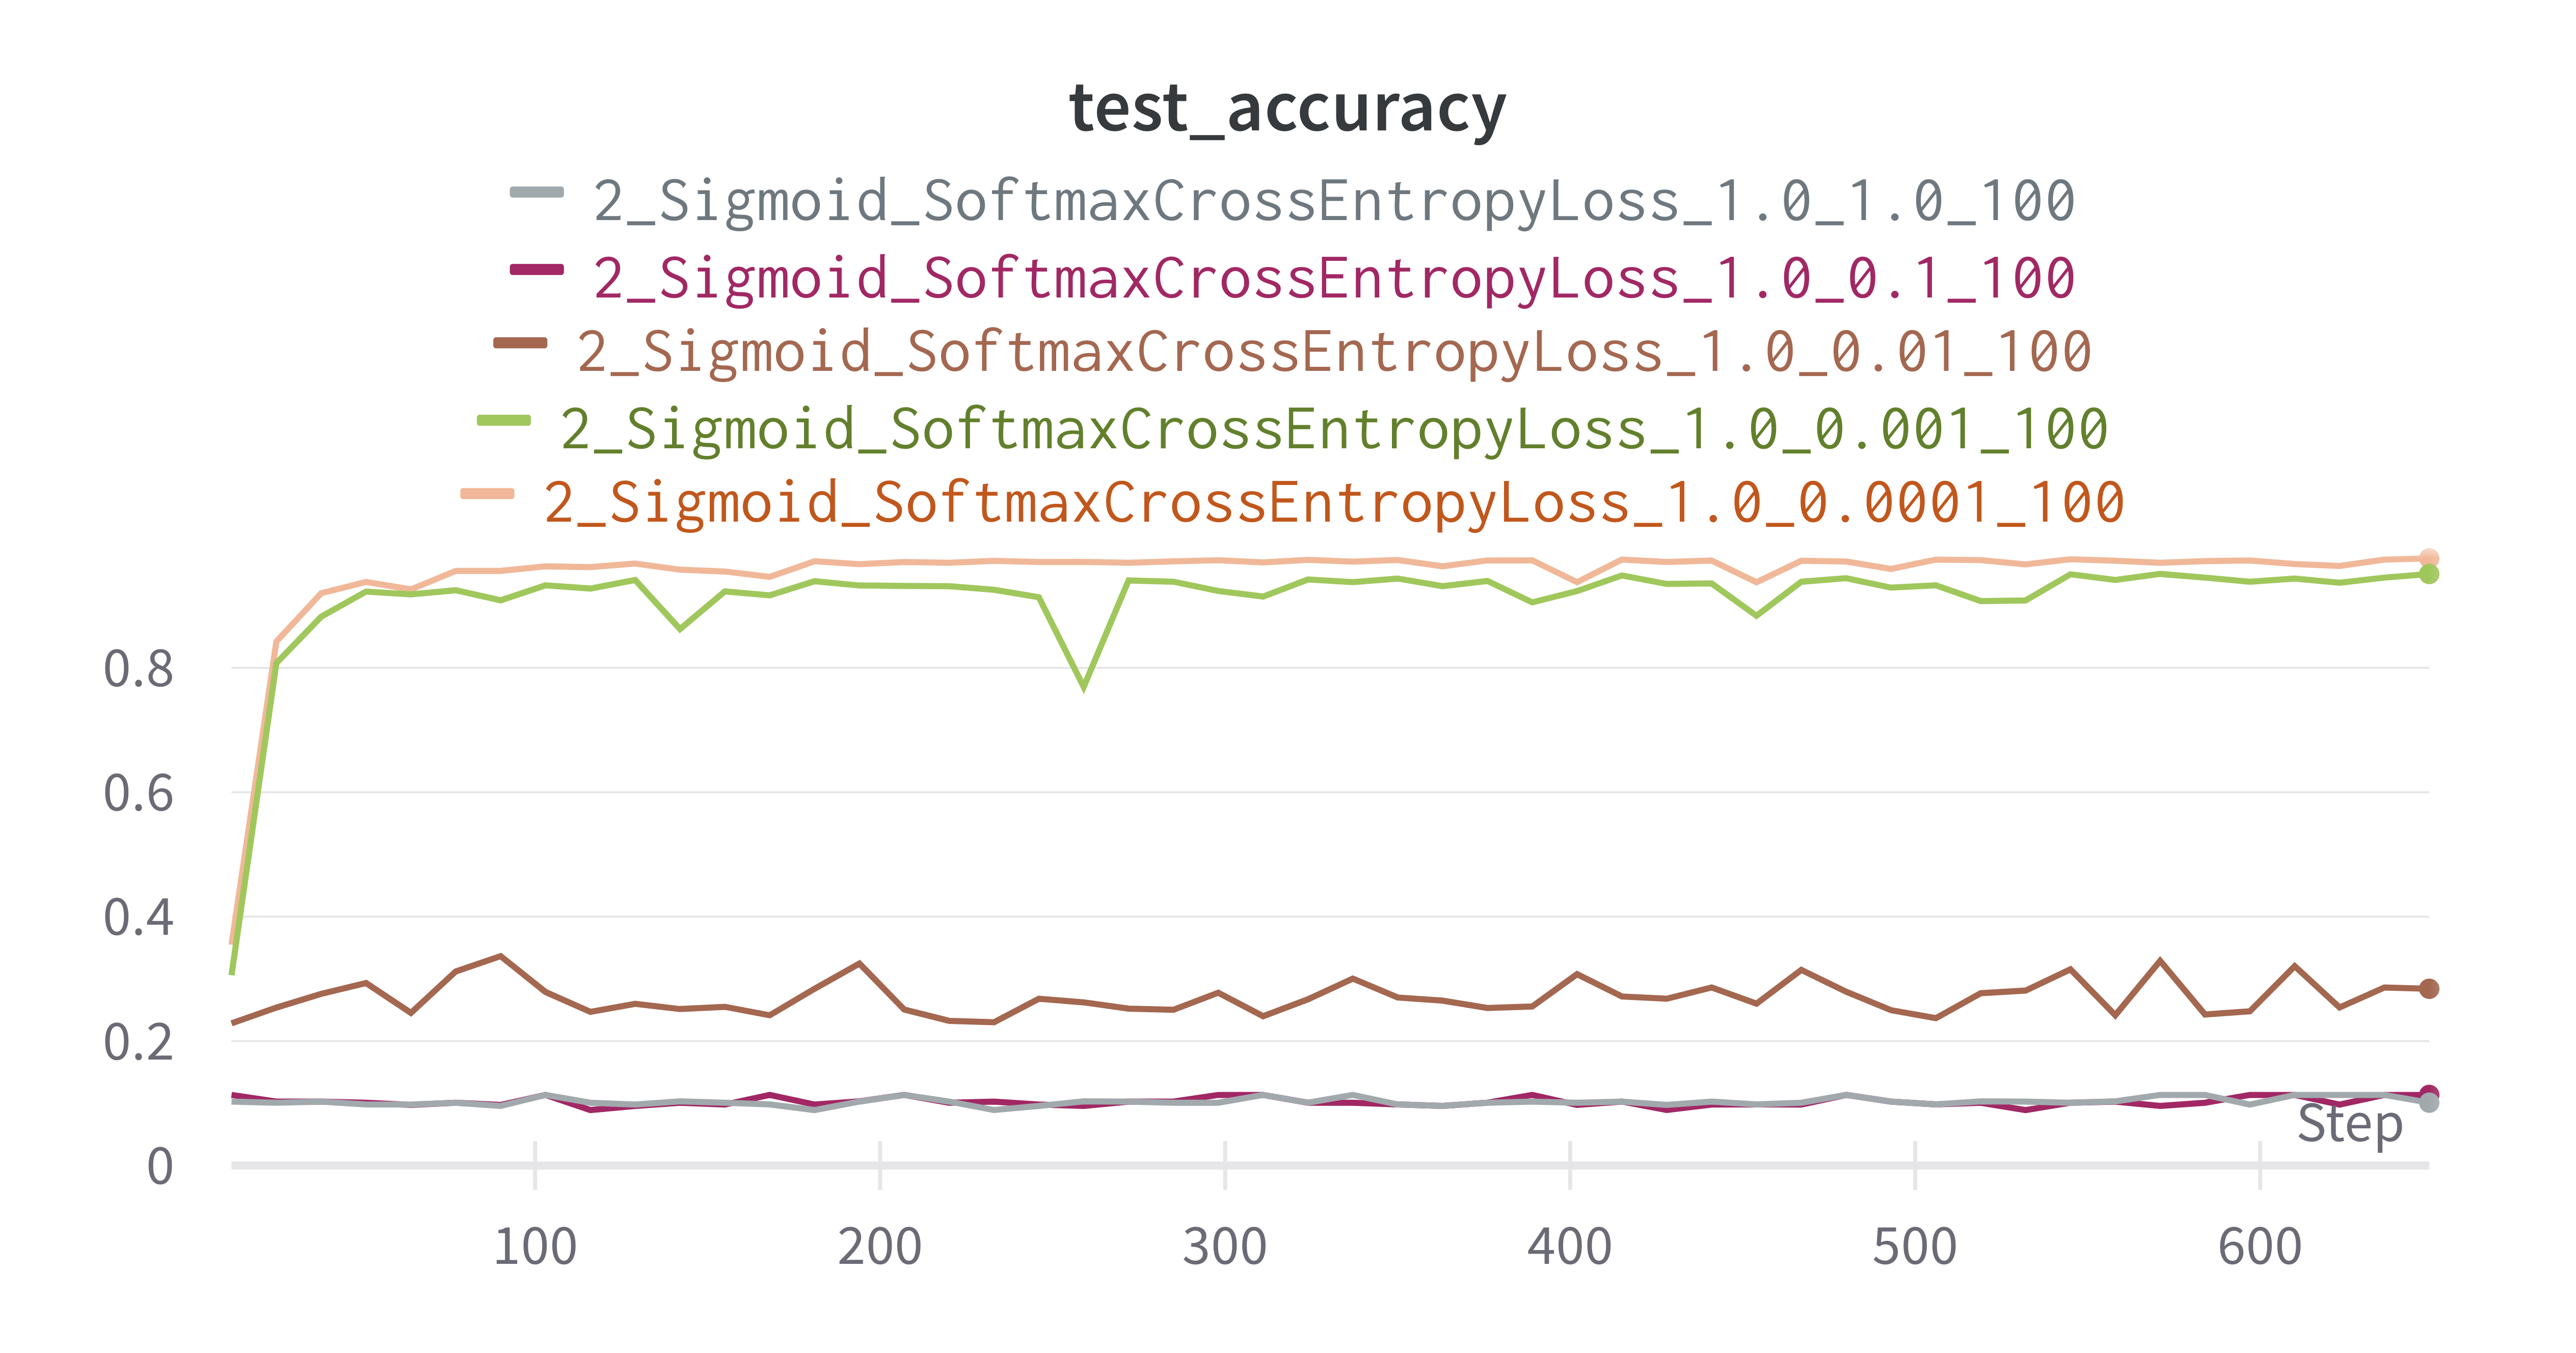
\includegraphics[width=1\textwidth]{../pics/消减率_2_Sigmoid_SoftmaxCross_test_acc.png}
		\caption{2\_Sigmoid\_Softmax 对比 test accuracy}
	\end{subfigure}
	\begin{subfigure}{0.475\textwidth}
		\centering
		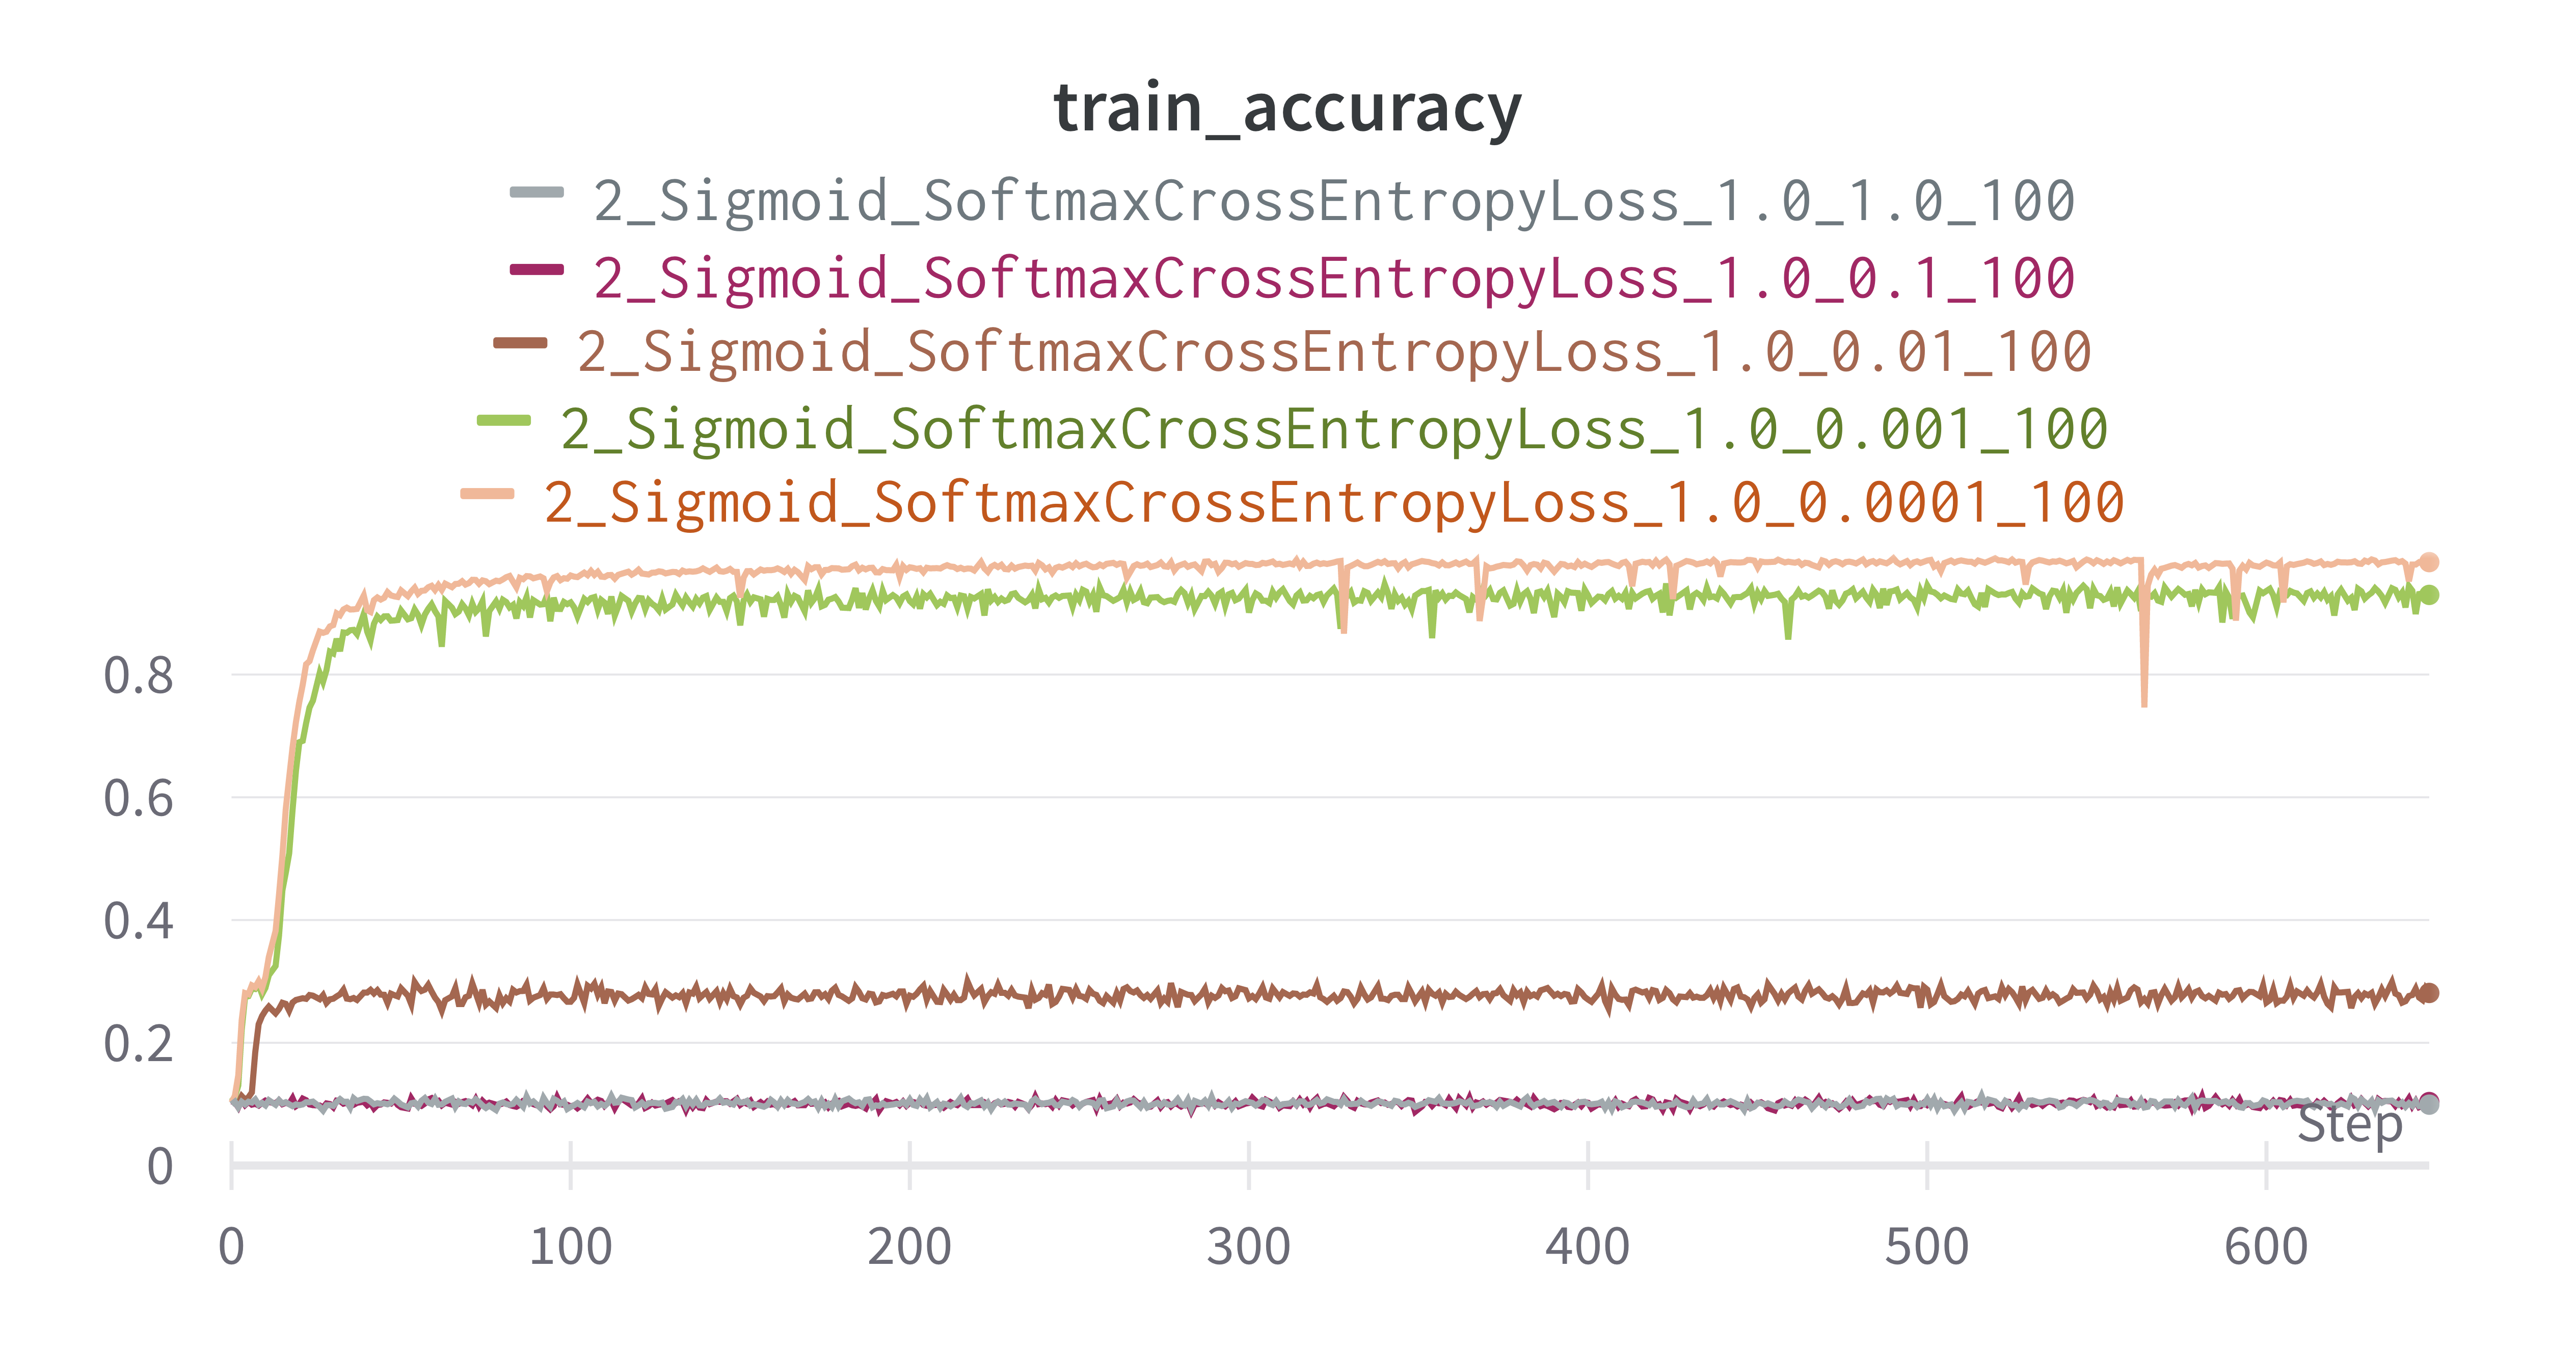
\includegraphics[width=1\textwidth]{../pics/消减率_2_Sigmoid_SoftmaxCross_train_acc.png}
		\caption{2\_Sigmoid\_Softmax 对比 train accuracy}
	\end{subfigure}
	\caption{基于 2\_Sigmoid\_Softmax 调节消减率}
	\label{fig:10}
\end{figure}

一般而言,权值消减(weight decay)的使用并不是为了提高准确率度也不是为了提高收敛速度,而是最终目的是防止过拟合。在损失函数中,weight decay 放置于正则项(regularization)前作为系数。一般而言,正则项表征模型的复杂度,weight decay 用于调节模型复杂度对损失函数的影响;若 weight decay 很大,则复杂的模型损失函数的值也就大,也即模型会倾向于减少参数值之和以避免过拟合。

从另一方面来讲,当过拟合现象并不明显时,提高 weight decay 反而会抑制降低模型的表达能力。考虑到本次作业之前的数个实验并未出现显著的过拟合现象,故而提高 weight decay 更有可能导致模型在有限的训练时间里失去表达能力。具体到 2\_Gelu\_HingeLoss 与 2\_Sigmoid\_Softmax 模型而言,本身在各自最优学习率的前提下,提高 weight decay 果然降低了模型的表达能力。可以观察到,模型的表达能力和 weight decay 基本负相关,当 weight decay 为 1 时,两个模型在测试集上的准确率均在 0.105 左右波动;对于十分类问题,这等价随机输出结果,符合期望。

\label{paragraph:1}

\subsection{批量大小影响}

模型选取 1\_Sigmoid\_EuclideanLoss 以 1e-2 为学习率(图 \ref{fig:11})与 2\_Sigmoid\_Softmax 以 1 为学习率(图 \ref{fig:12}),消减率均选取为 0。以\{10, 20, 50, 100, 200\} 为批量大小,展开批量大小对比实验。

\begin{figure}[htbp]
	\centering
	\begin{subfigure}{0.475\textwidth}
		\centering
		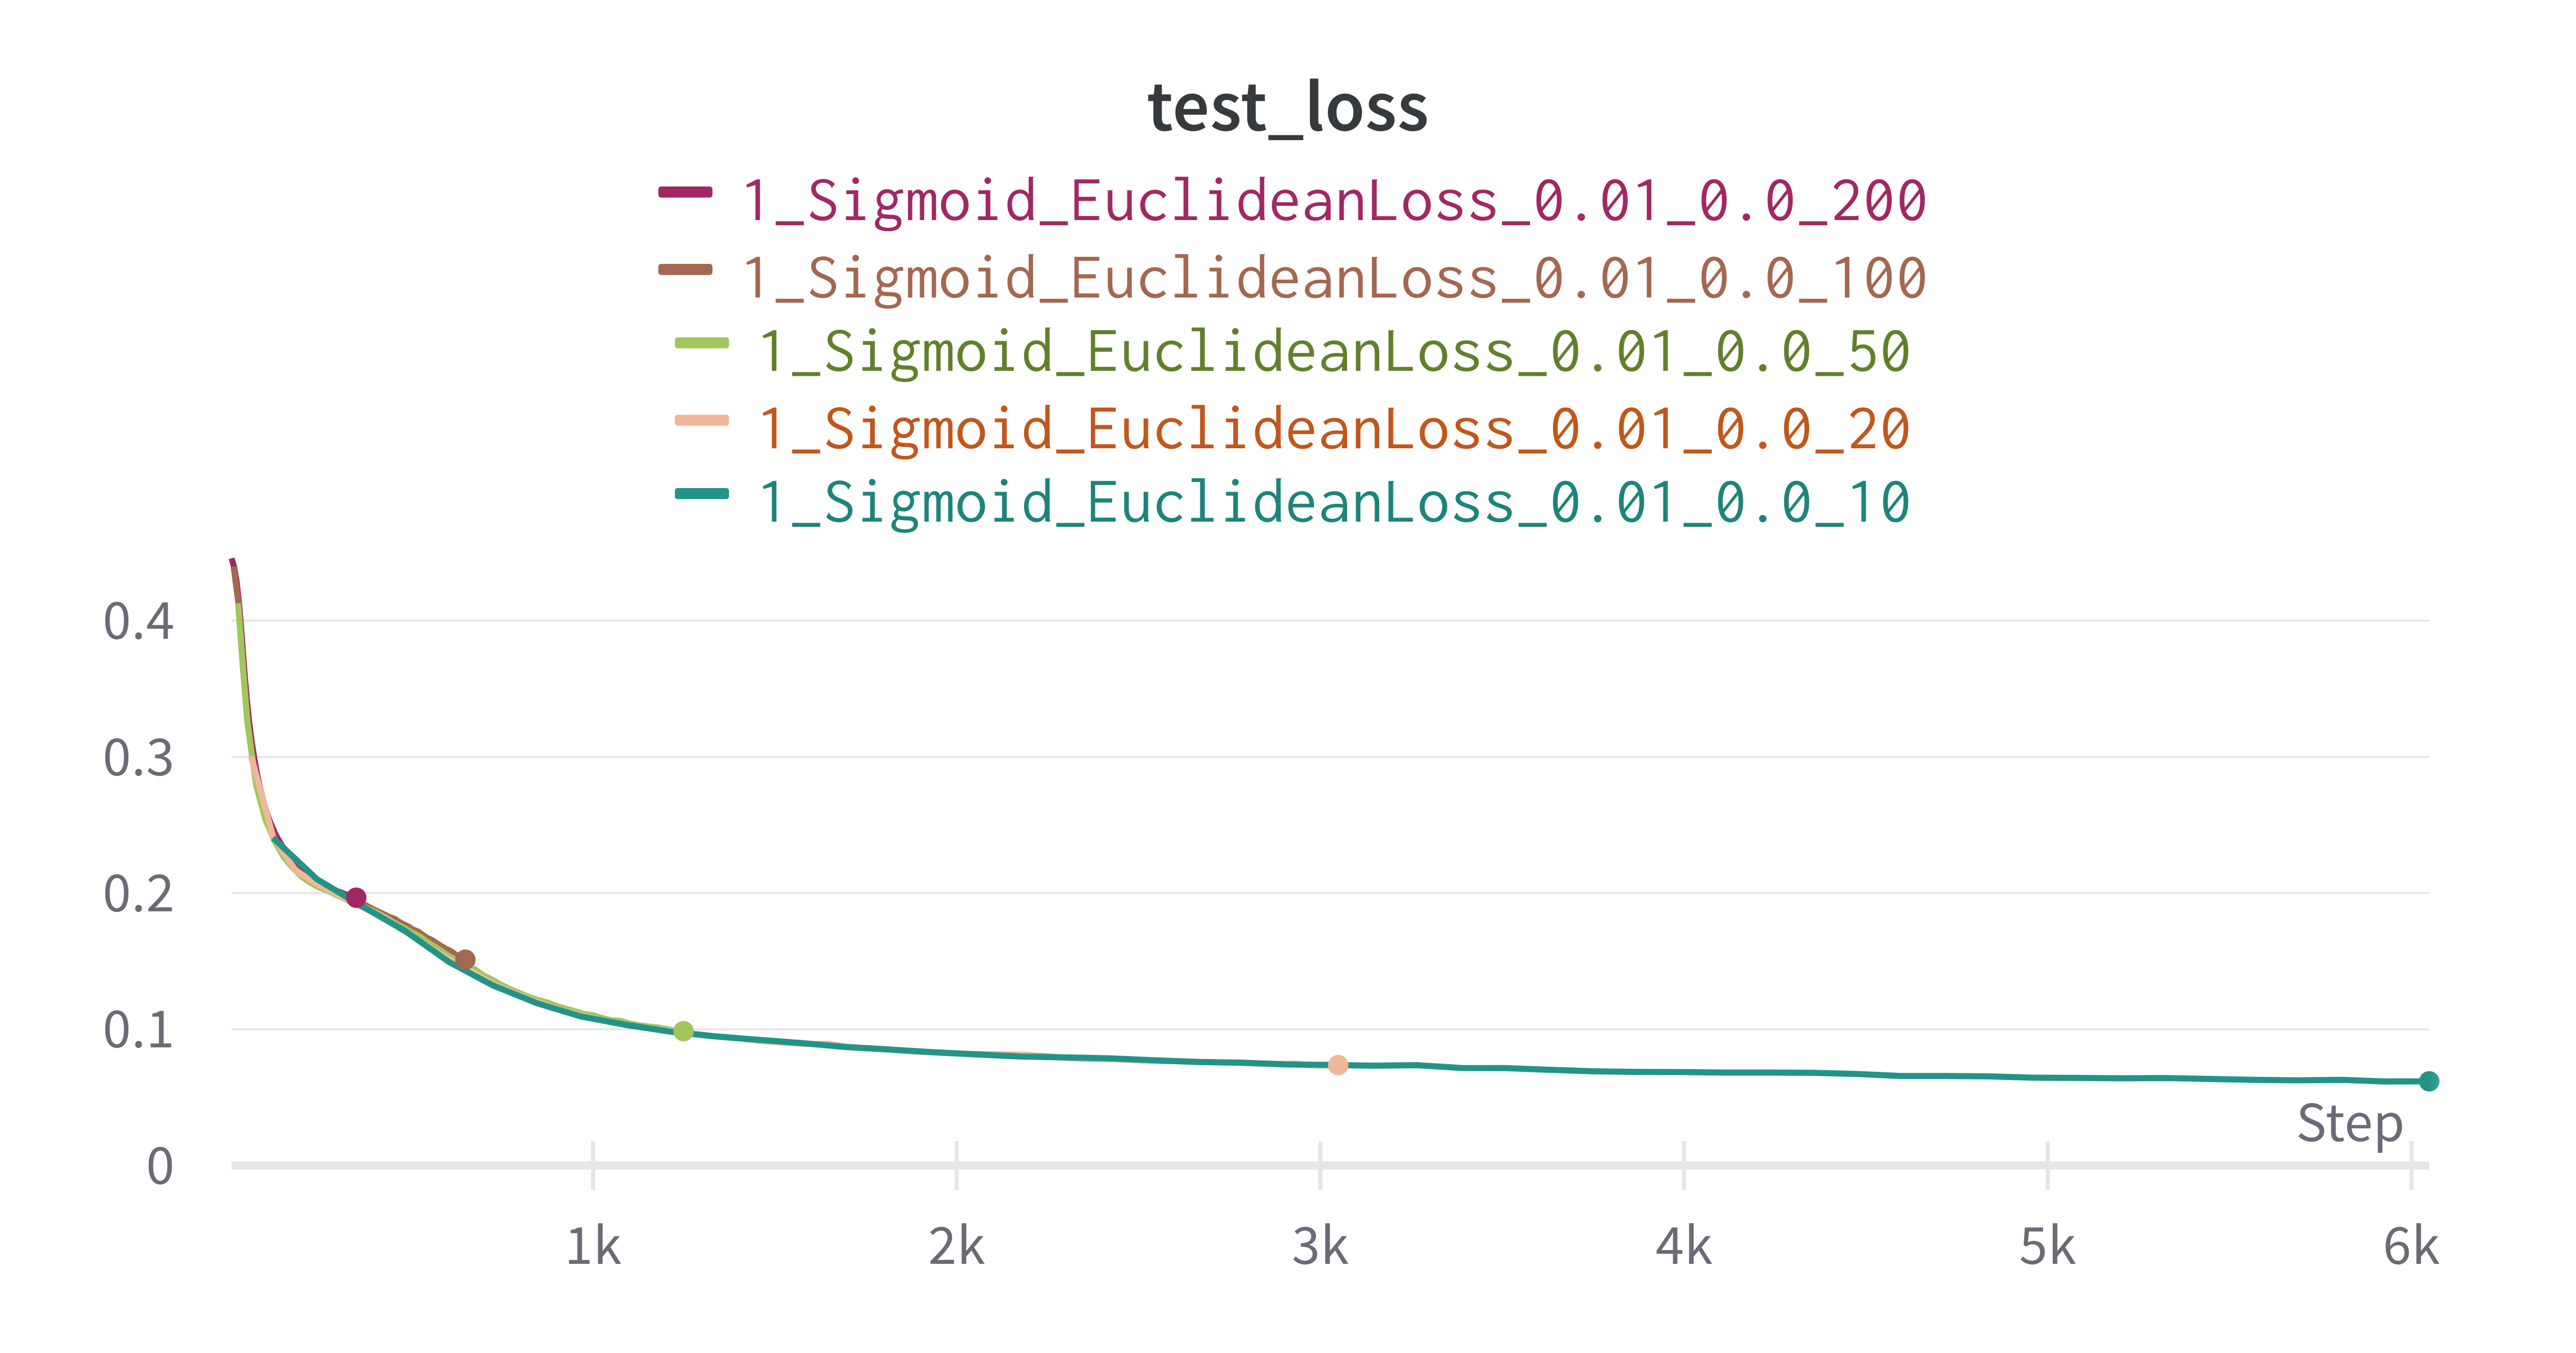
\includegraphics[width=1\textwidth]{../pics/批量_1_Sigmoid_EuclideanLoss_test_loss.png}
		\caption{1\_Sigmoid\_EuclideanLoss 对比 test loss}
	\end{subfigure}
	\begin{subfigure}{0.475\textwidth}
		\centering
		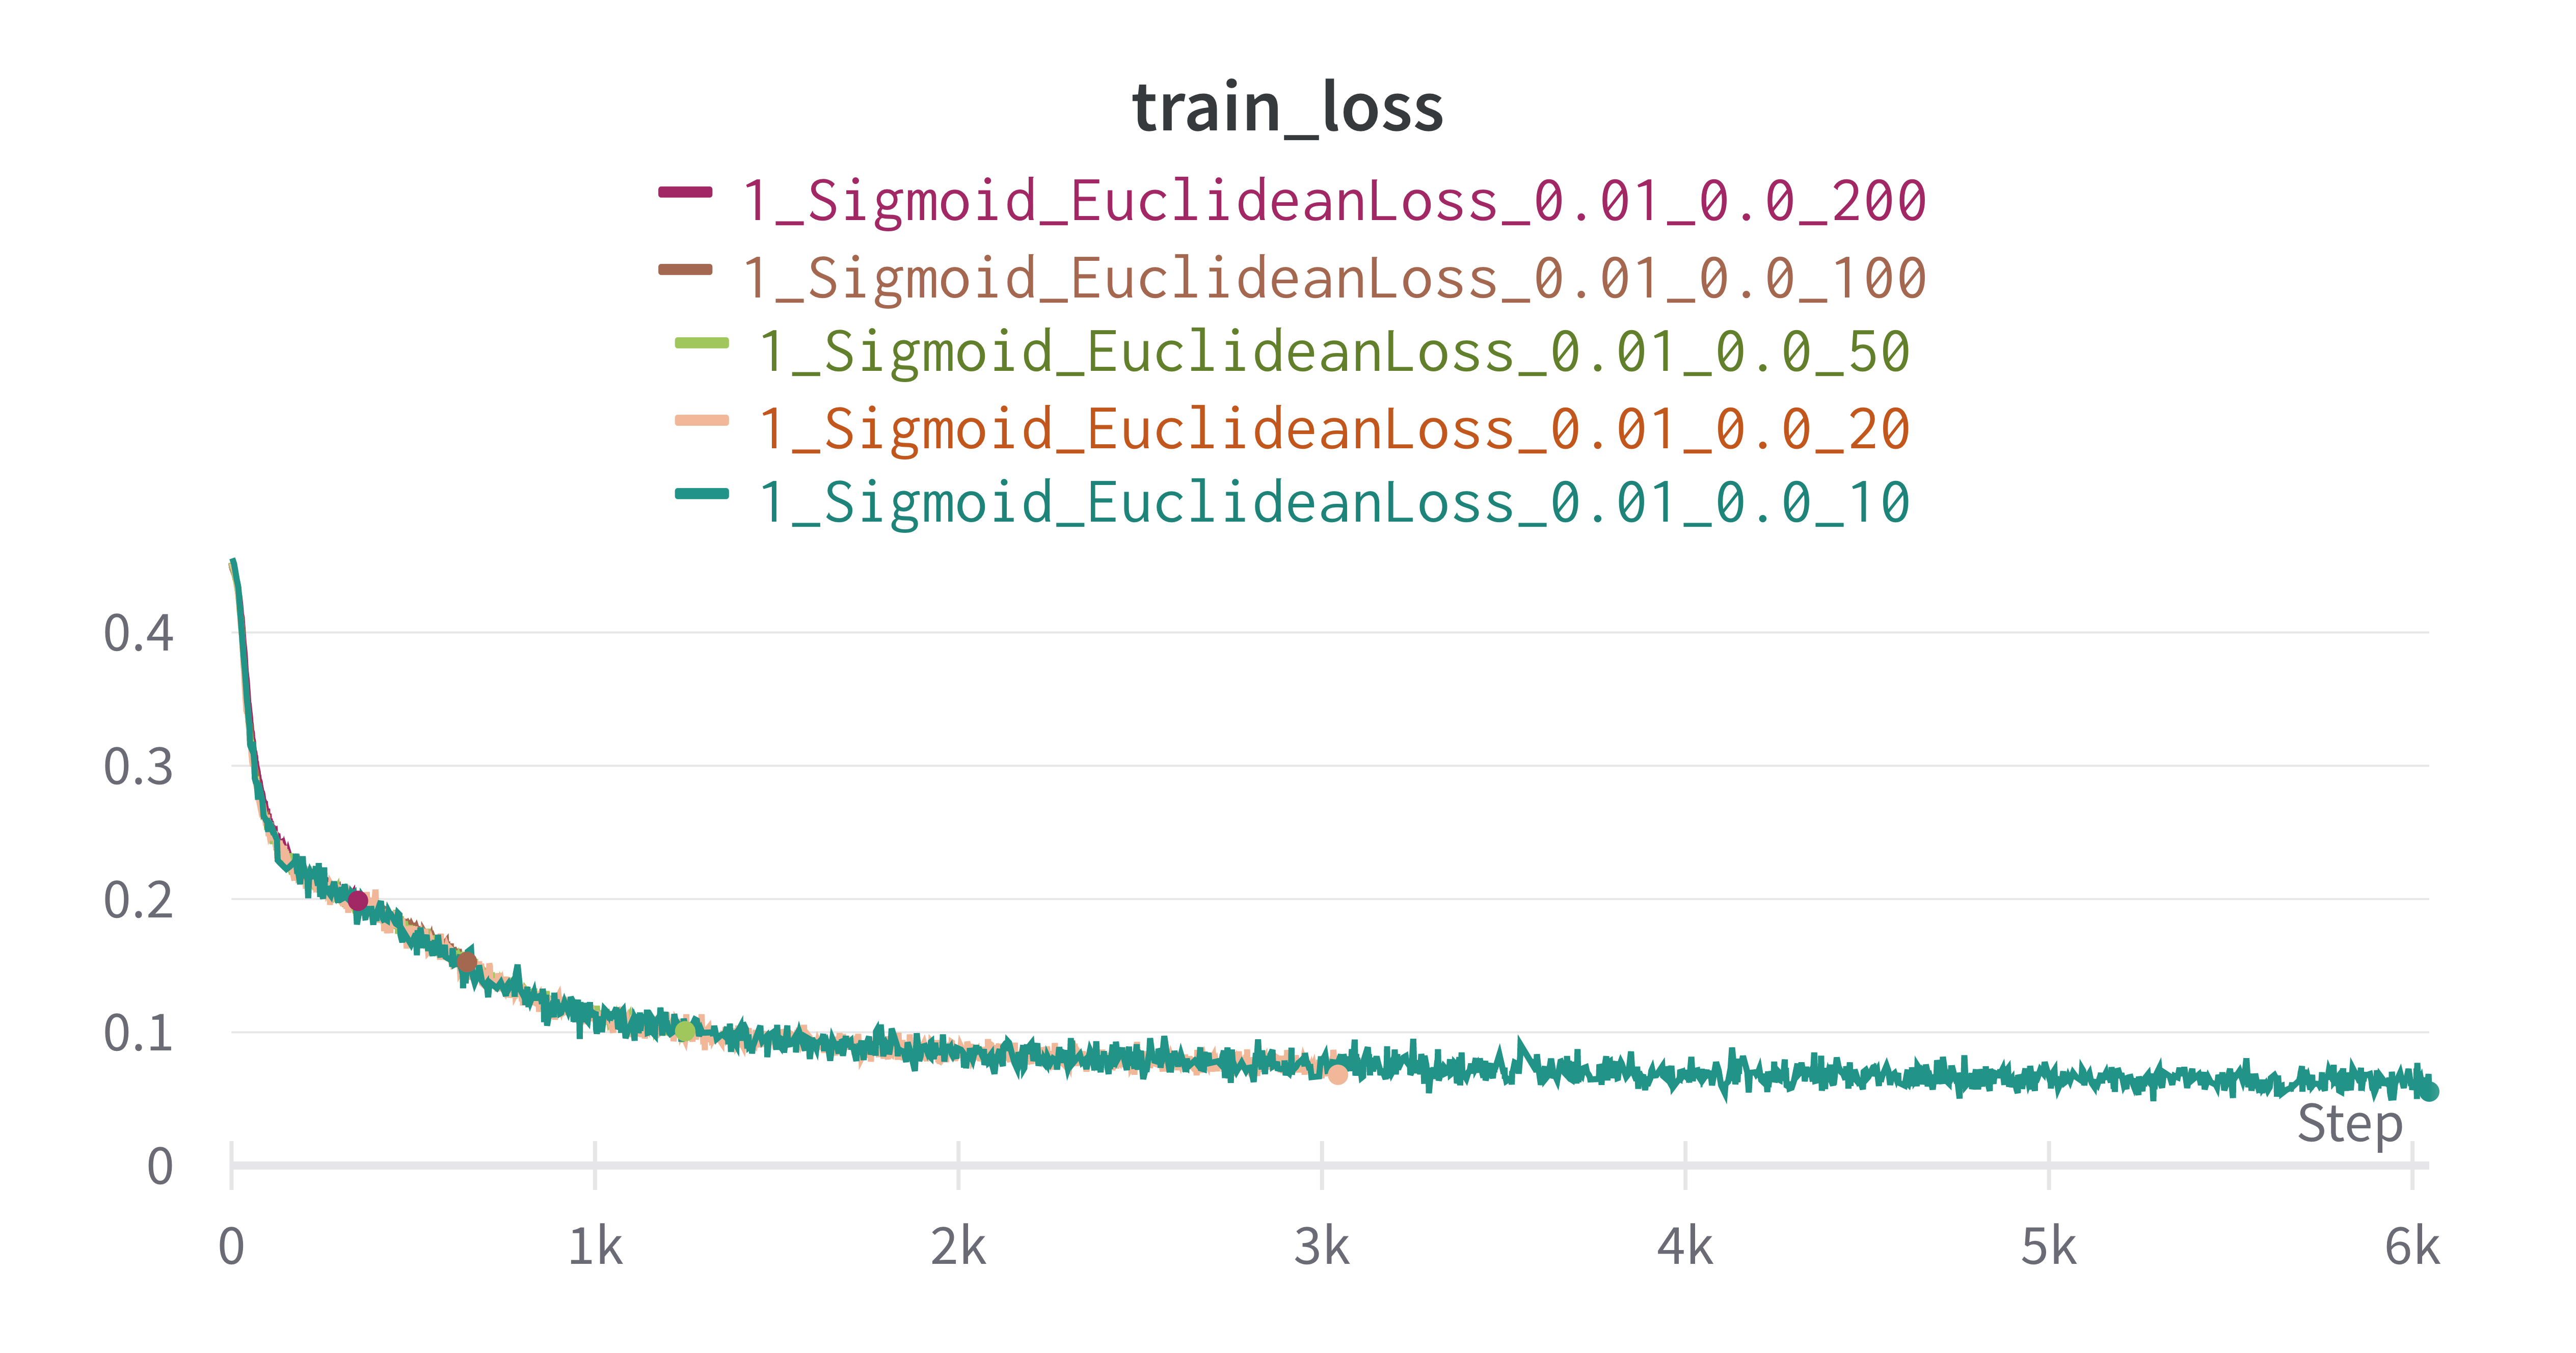
\includegraphics[width=1\textwidth]{../pics/批量_1_Sigmoid_EuclideanLoss_train_loss.png}
		\caption{1\_Sigmoid\_EuclideanLoss 对比 train loss}
	\end{subfigure}
	\begin{subfigure}{0.475\textwidth}
		\centering
		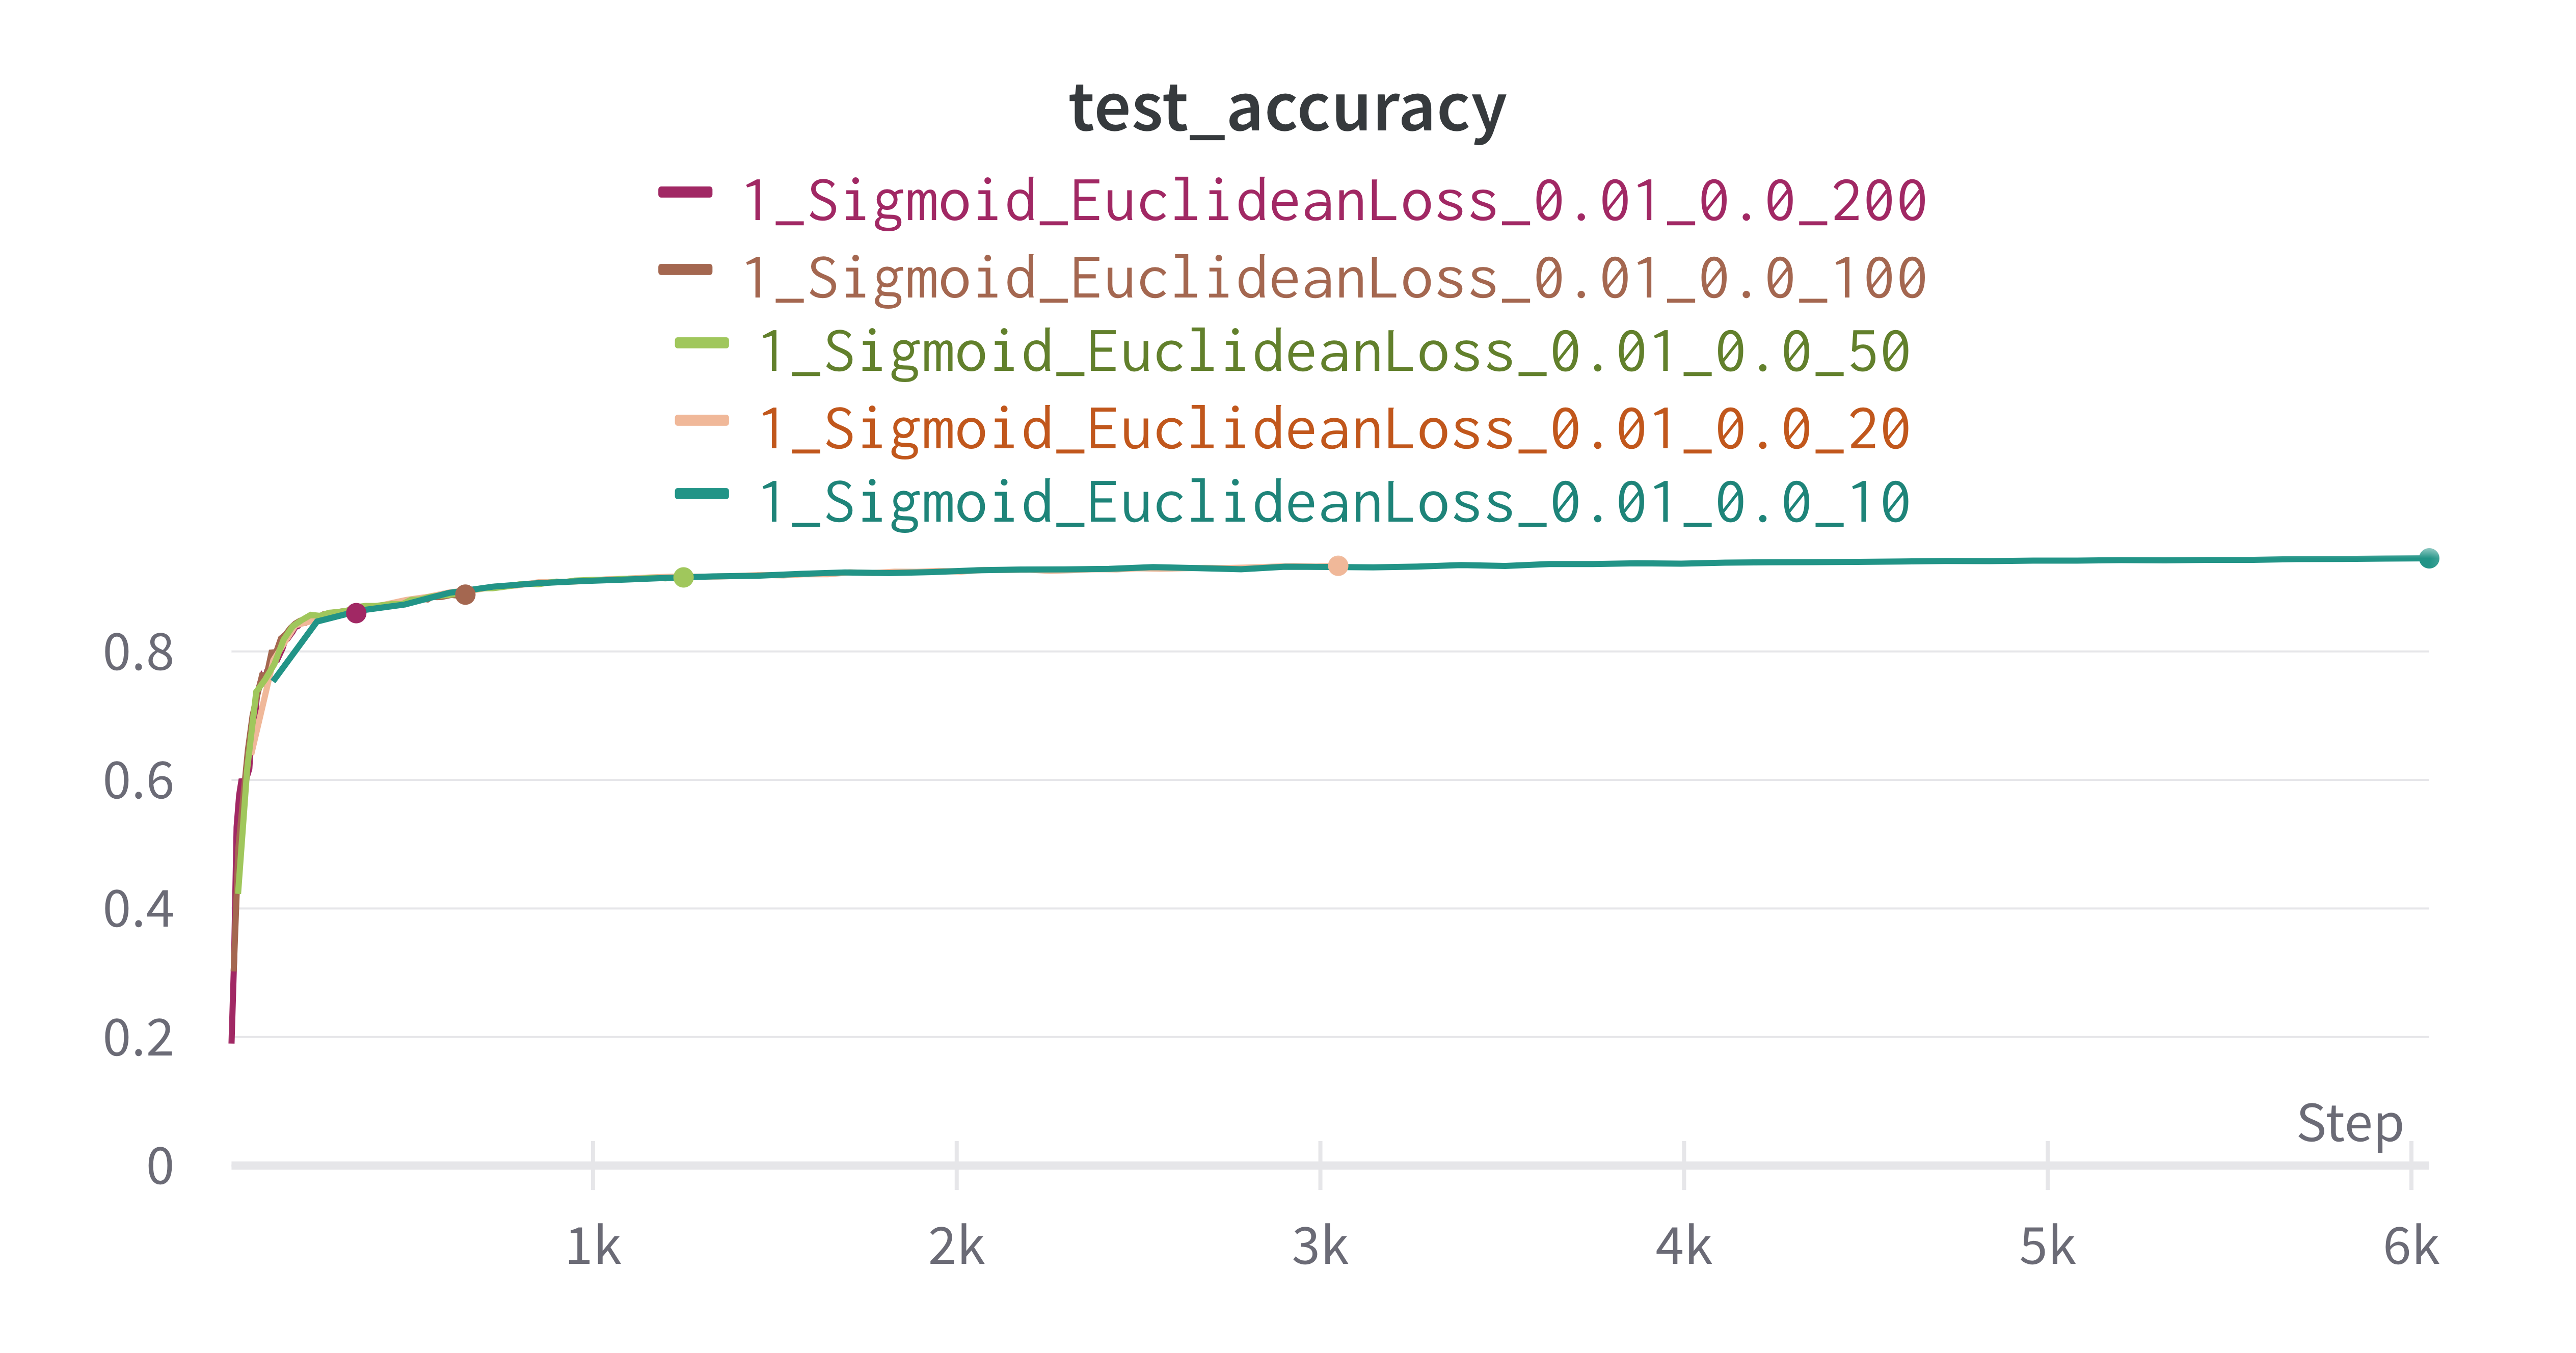
\includegraphics[width=1\textwidth]{../pics/批量_1_Sigmoid_EuclideanLoss_test_acc.png}
		\caption{1\_Sigmoid\_EuclideanLoss 对比 test accuracy}
	\end{subfigure}
	\begin{subfigure}{0.475\textwidth}
		\centering
		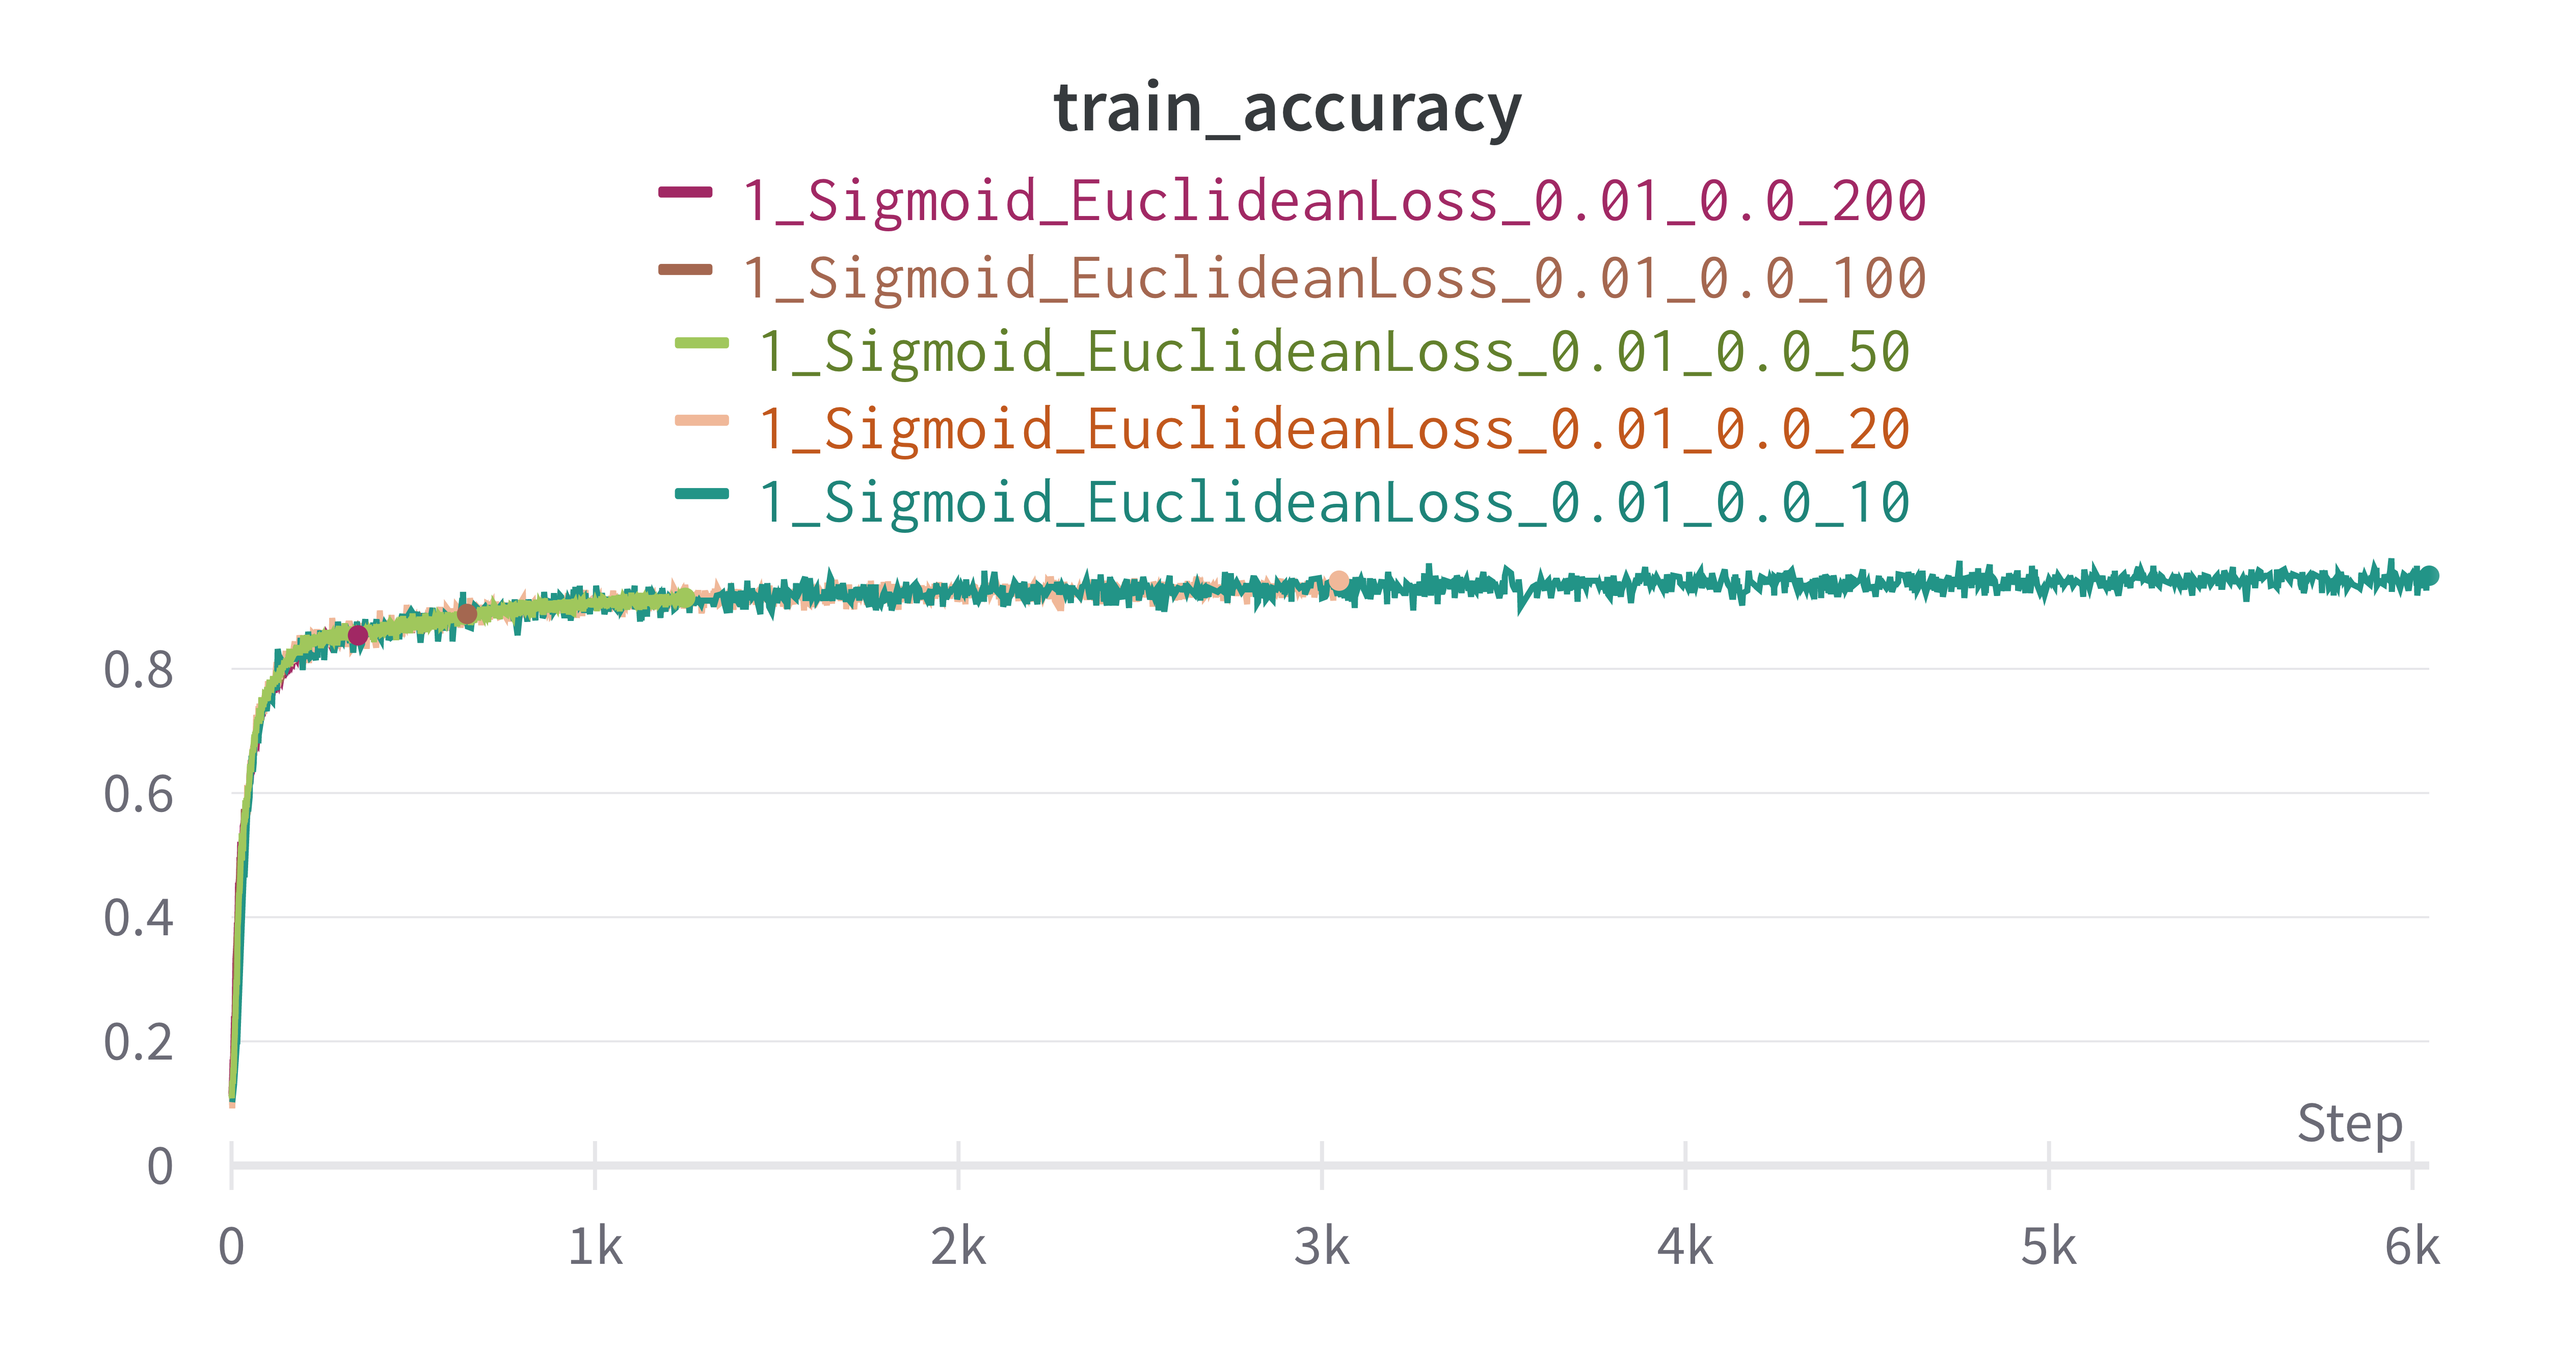
\includegraphics[width=1\textwidth]{../pics/批量_1_Sigmoid_EuclideanLoss_train_acc.png}
		\caption{1\_Sigmoid\_EuclideanLoss  对比 train accuracy}
	\end{subfigure}
	\caption{基于 1\_Sigmoid\_EuclideanLoss  调节批量大小}
	\label{fig:11}
\end{figure}

\begin{figure}[htbp]
	\centering
	\begin{subfigure}{0.475\textwidth}
		\centering
		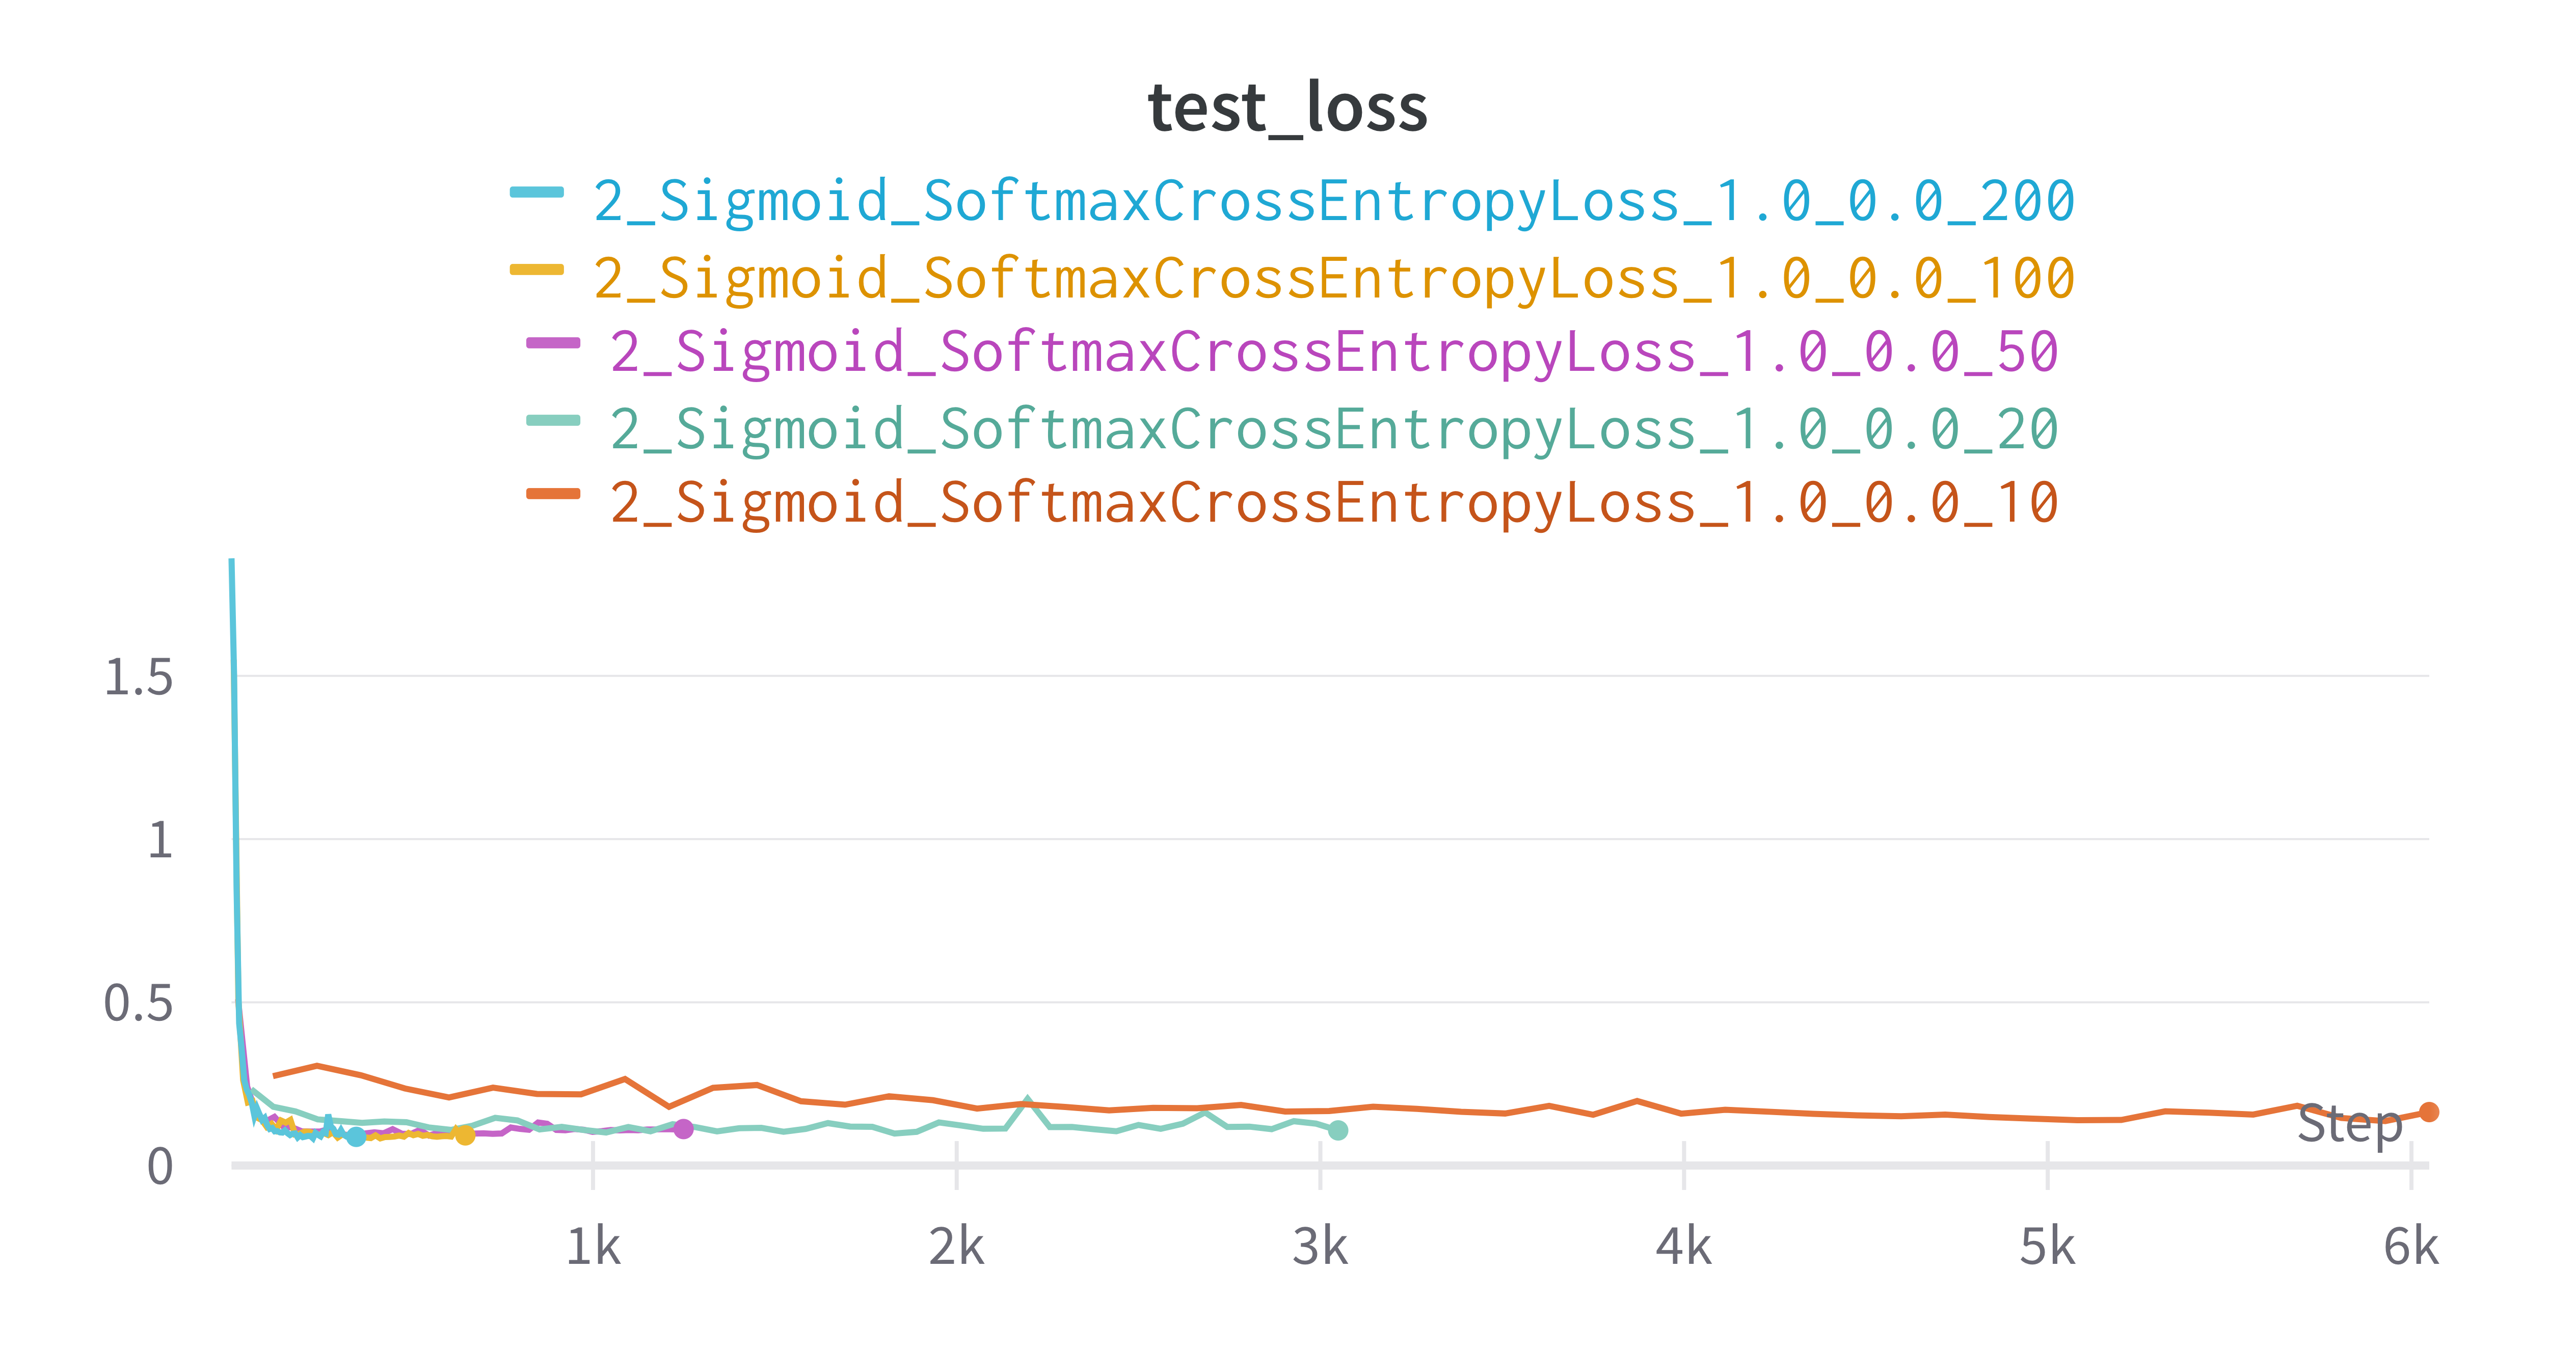
\includegraphics[width=1\textwidth]{../pics/批量大小_2_Sigmoid_Softmax_test_loss.png}
		\caption{2\_Sigmoid\_Softmax 对比 test loss}
	\end{subfigure}
	\begin{subfigure}{0.475\textwidth}
		\centering
		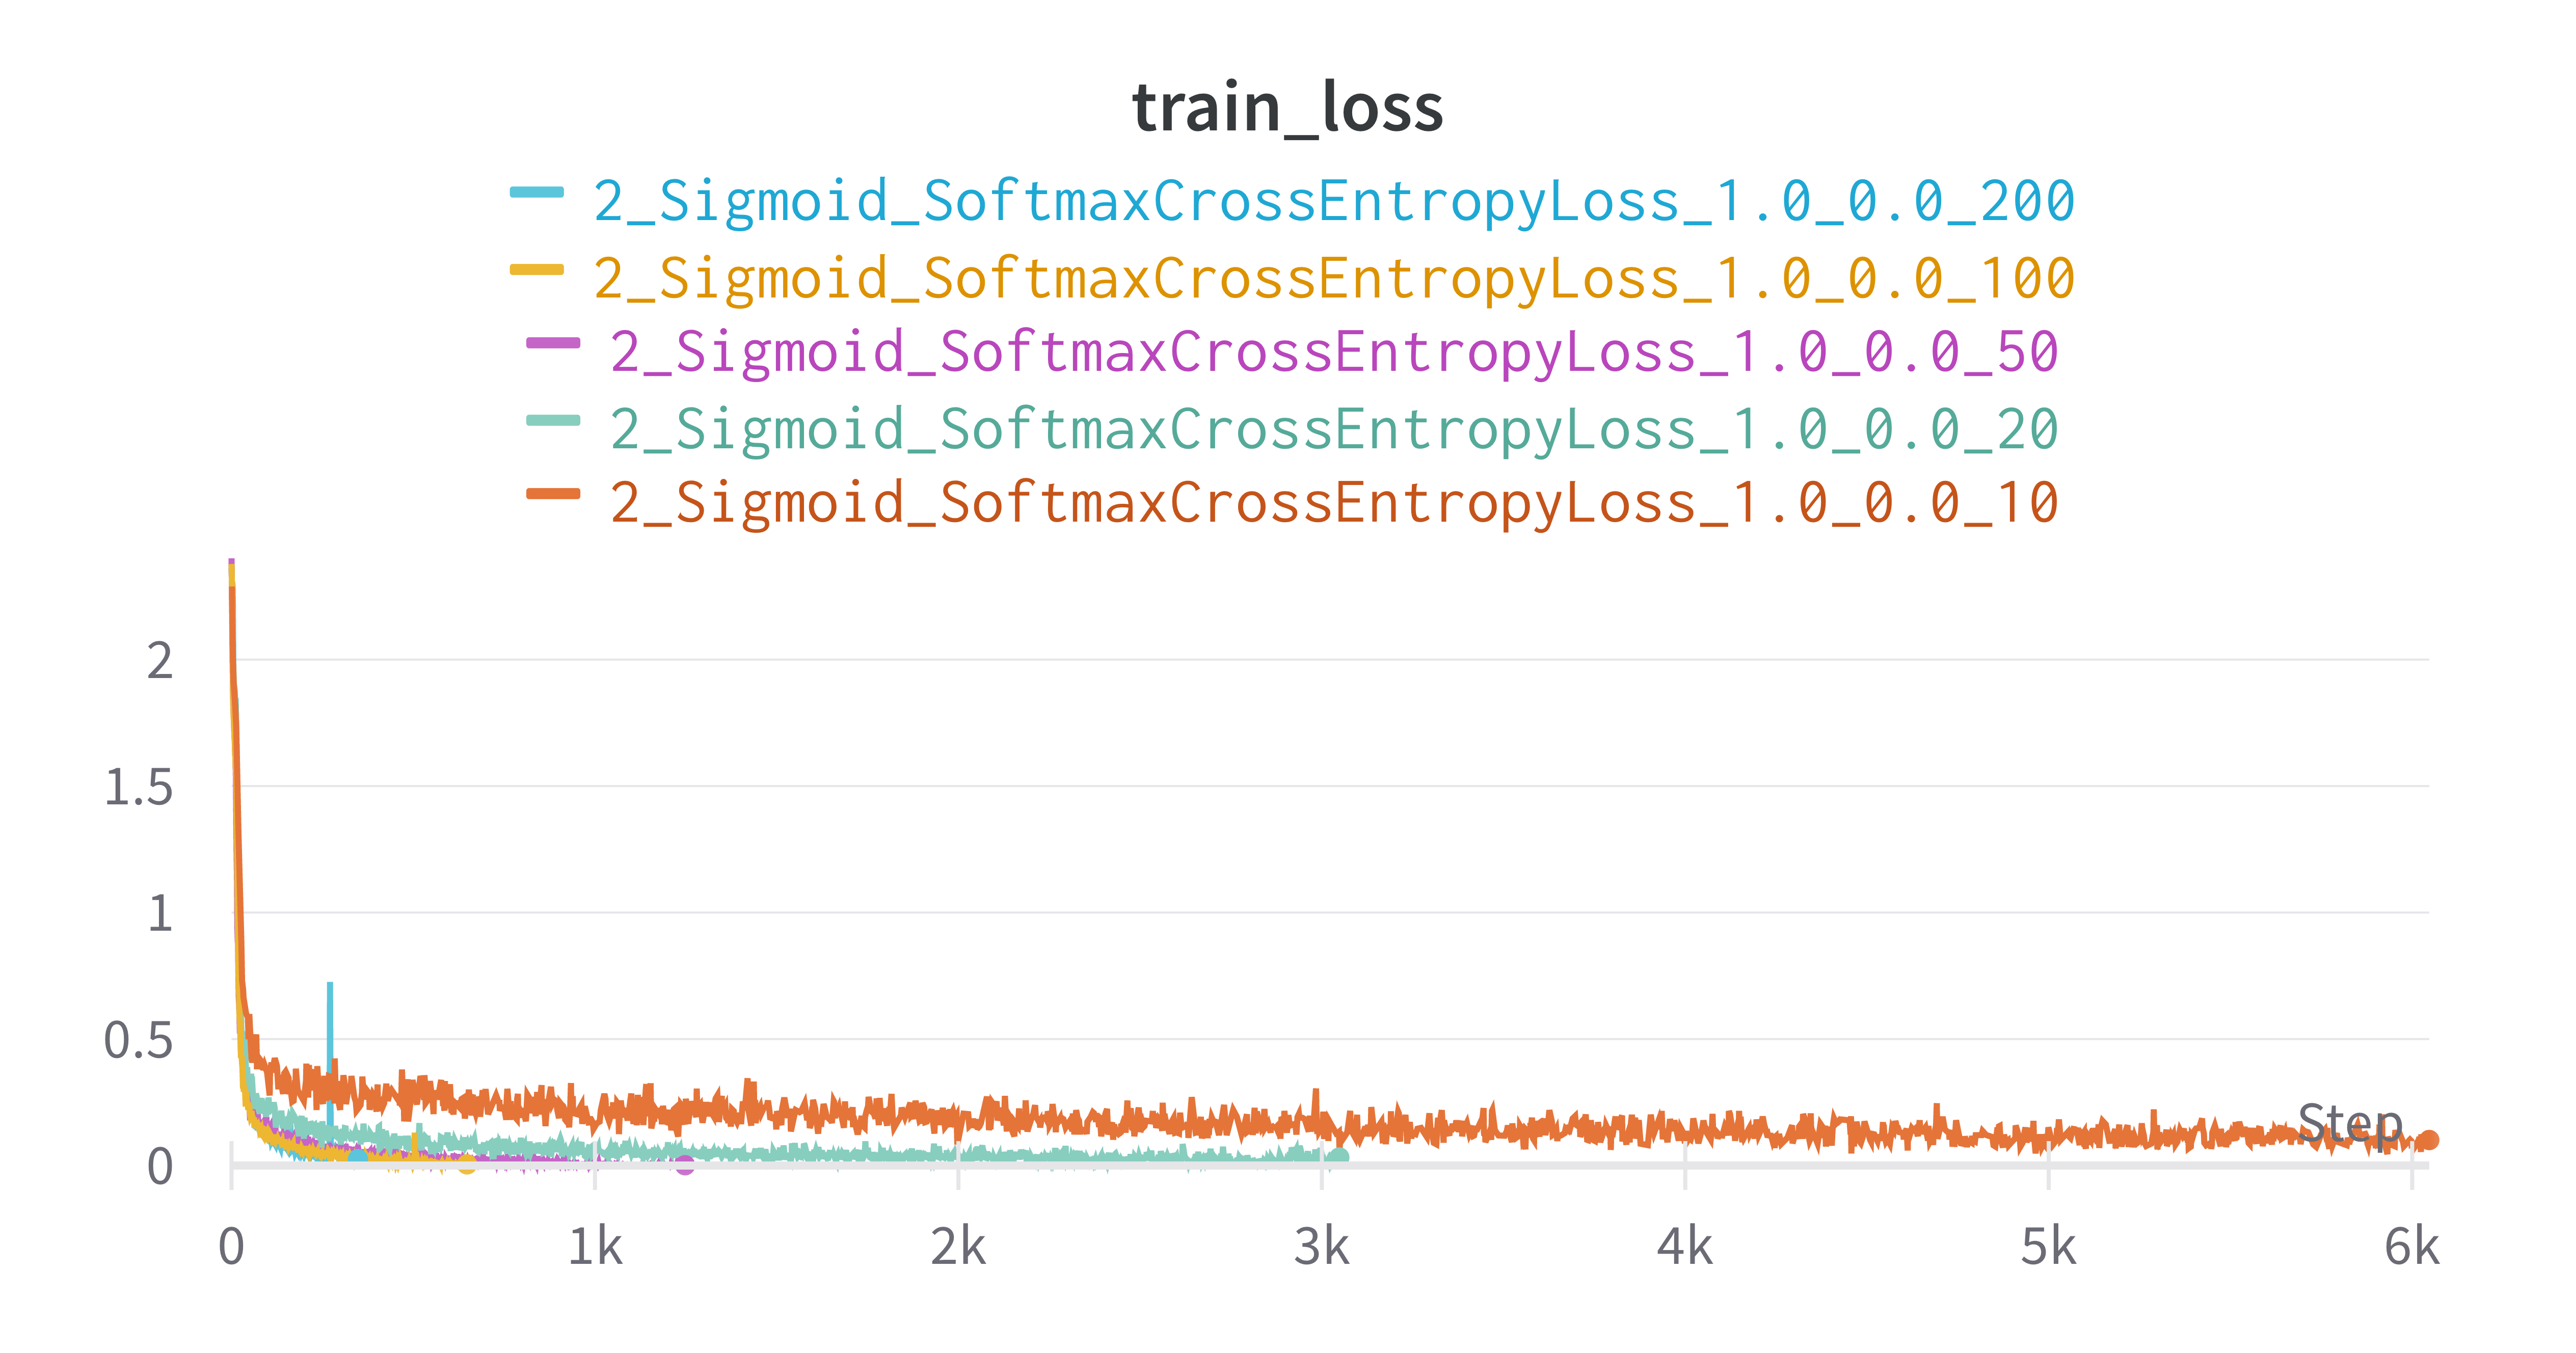
\includegraphics[width=1\textwidth]{../pics/批量大小_2_Sigmoid_Softmax_train_loss.png}
		\caption{2\_Sigmoid\_Softmax 对比 train loss}
	\end{subfigure}
	\begin{subfigure}{0.475\textwidth}
		\centering
		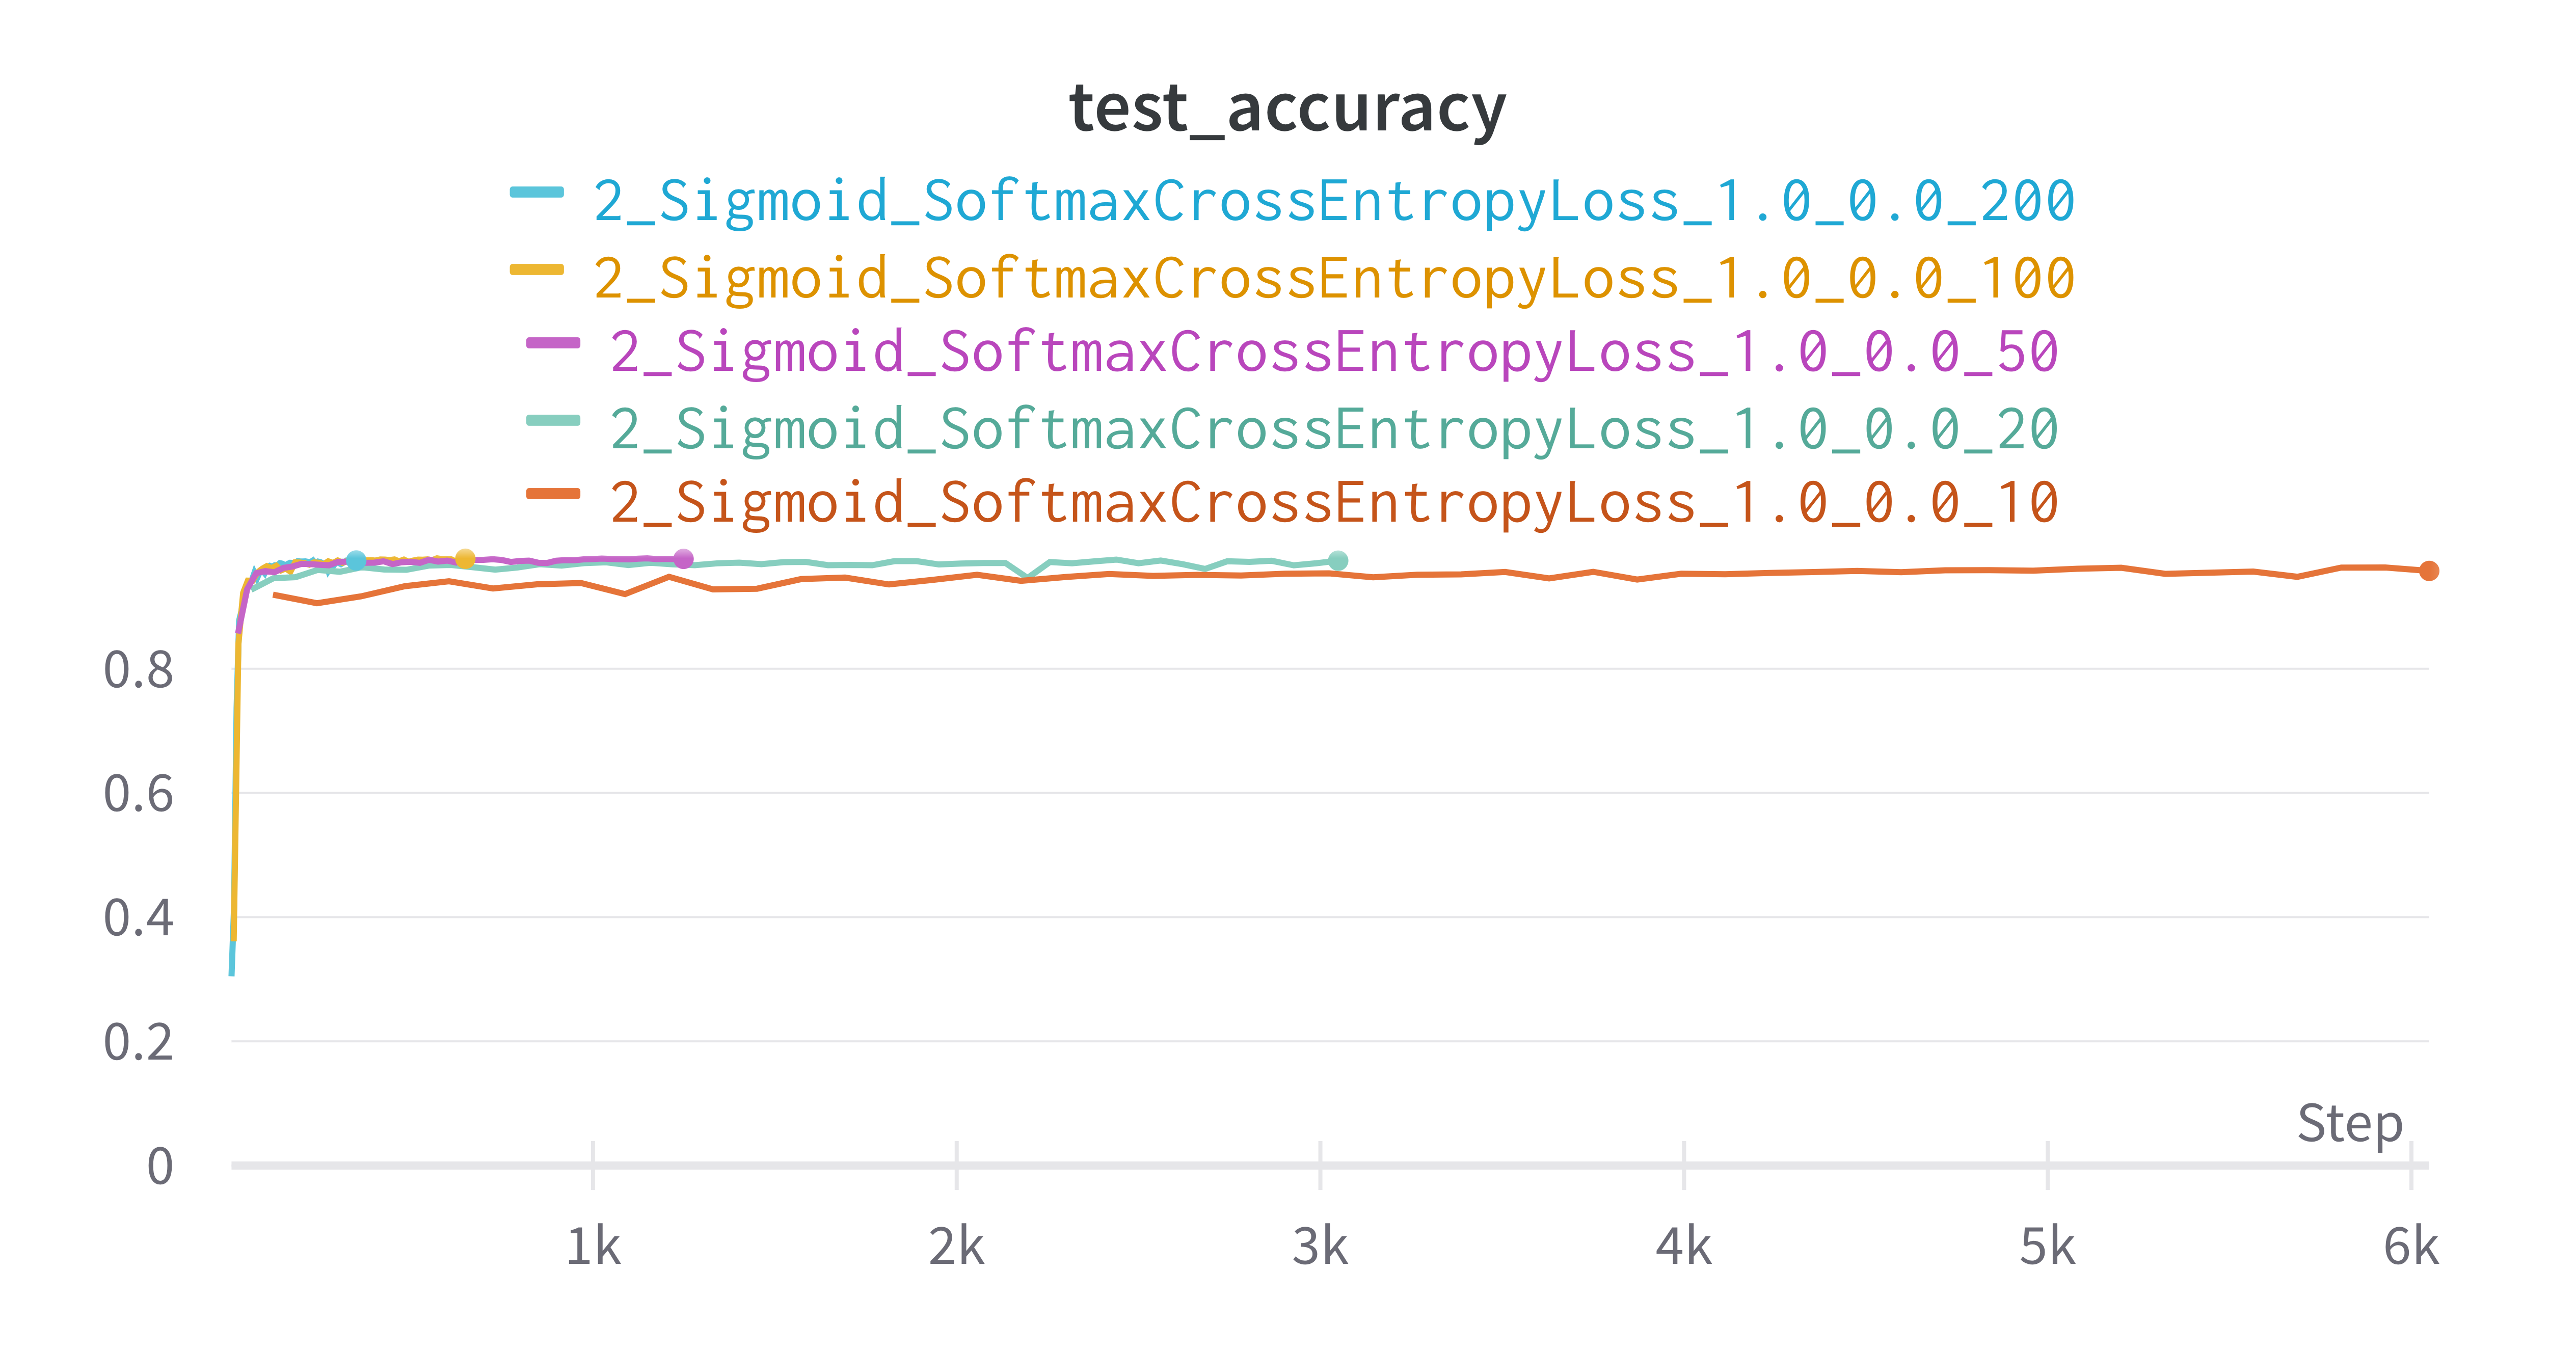
\includegraphics[width=1\textwidth]{../pics/批量大小_2_Sigmoid_Softmax_test_acc.png}
		\caption{2\_Sigmoid\_Softmax 对比 test accuracy}
	\end{subfigure}
	\begin{subfigure}{0.475\textwidth}
		\centering
		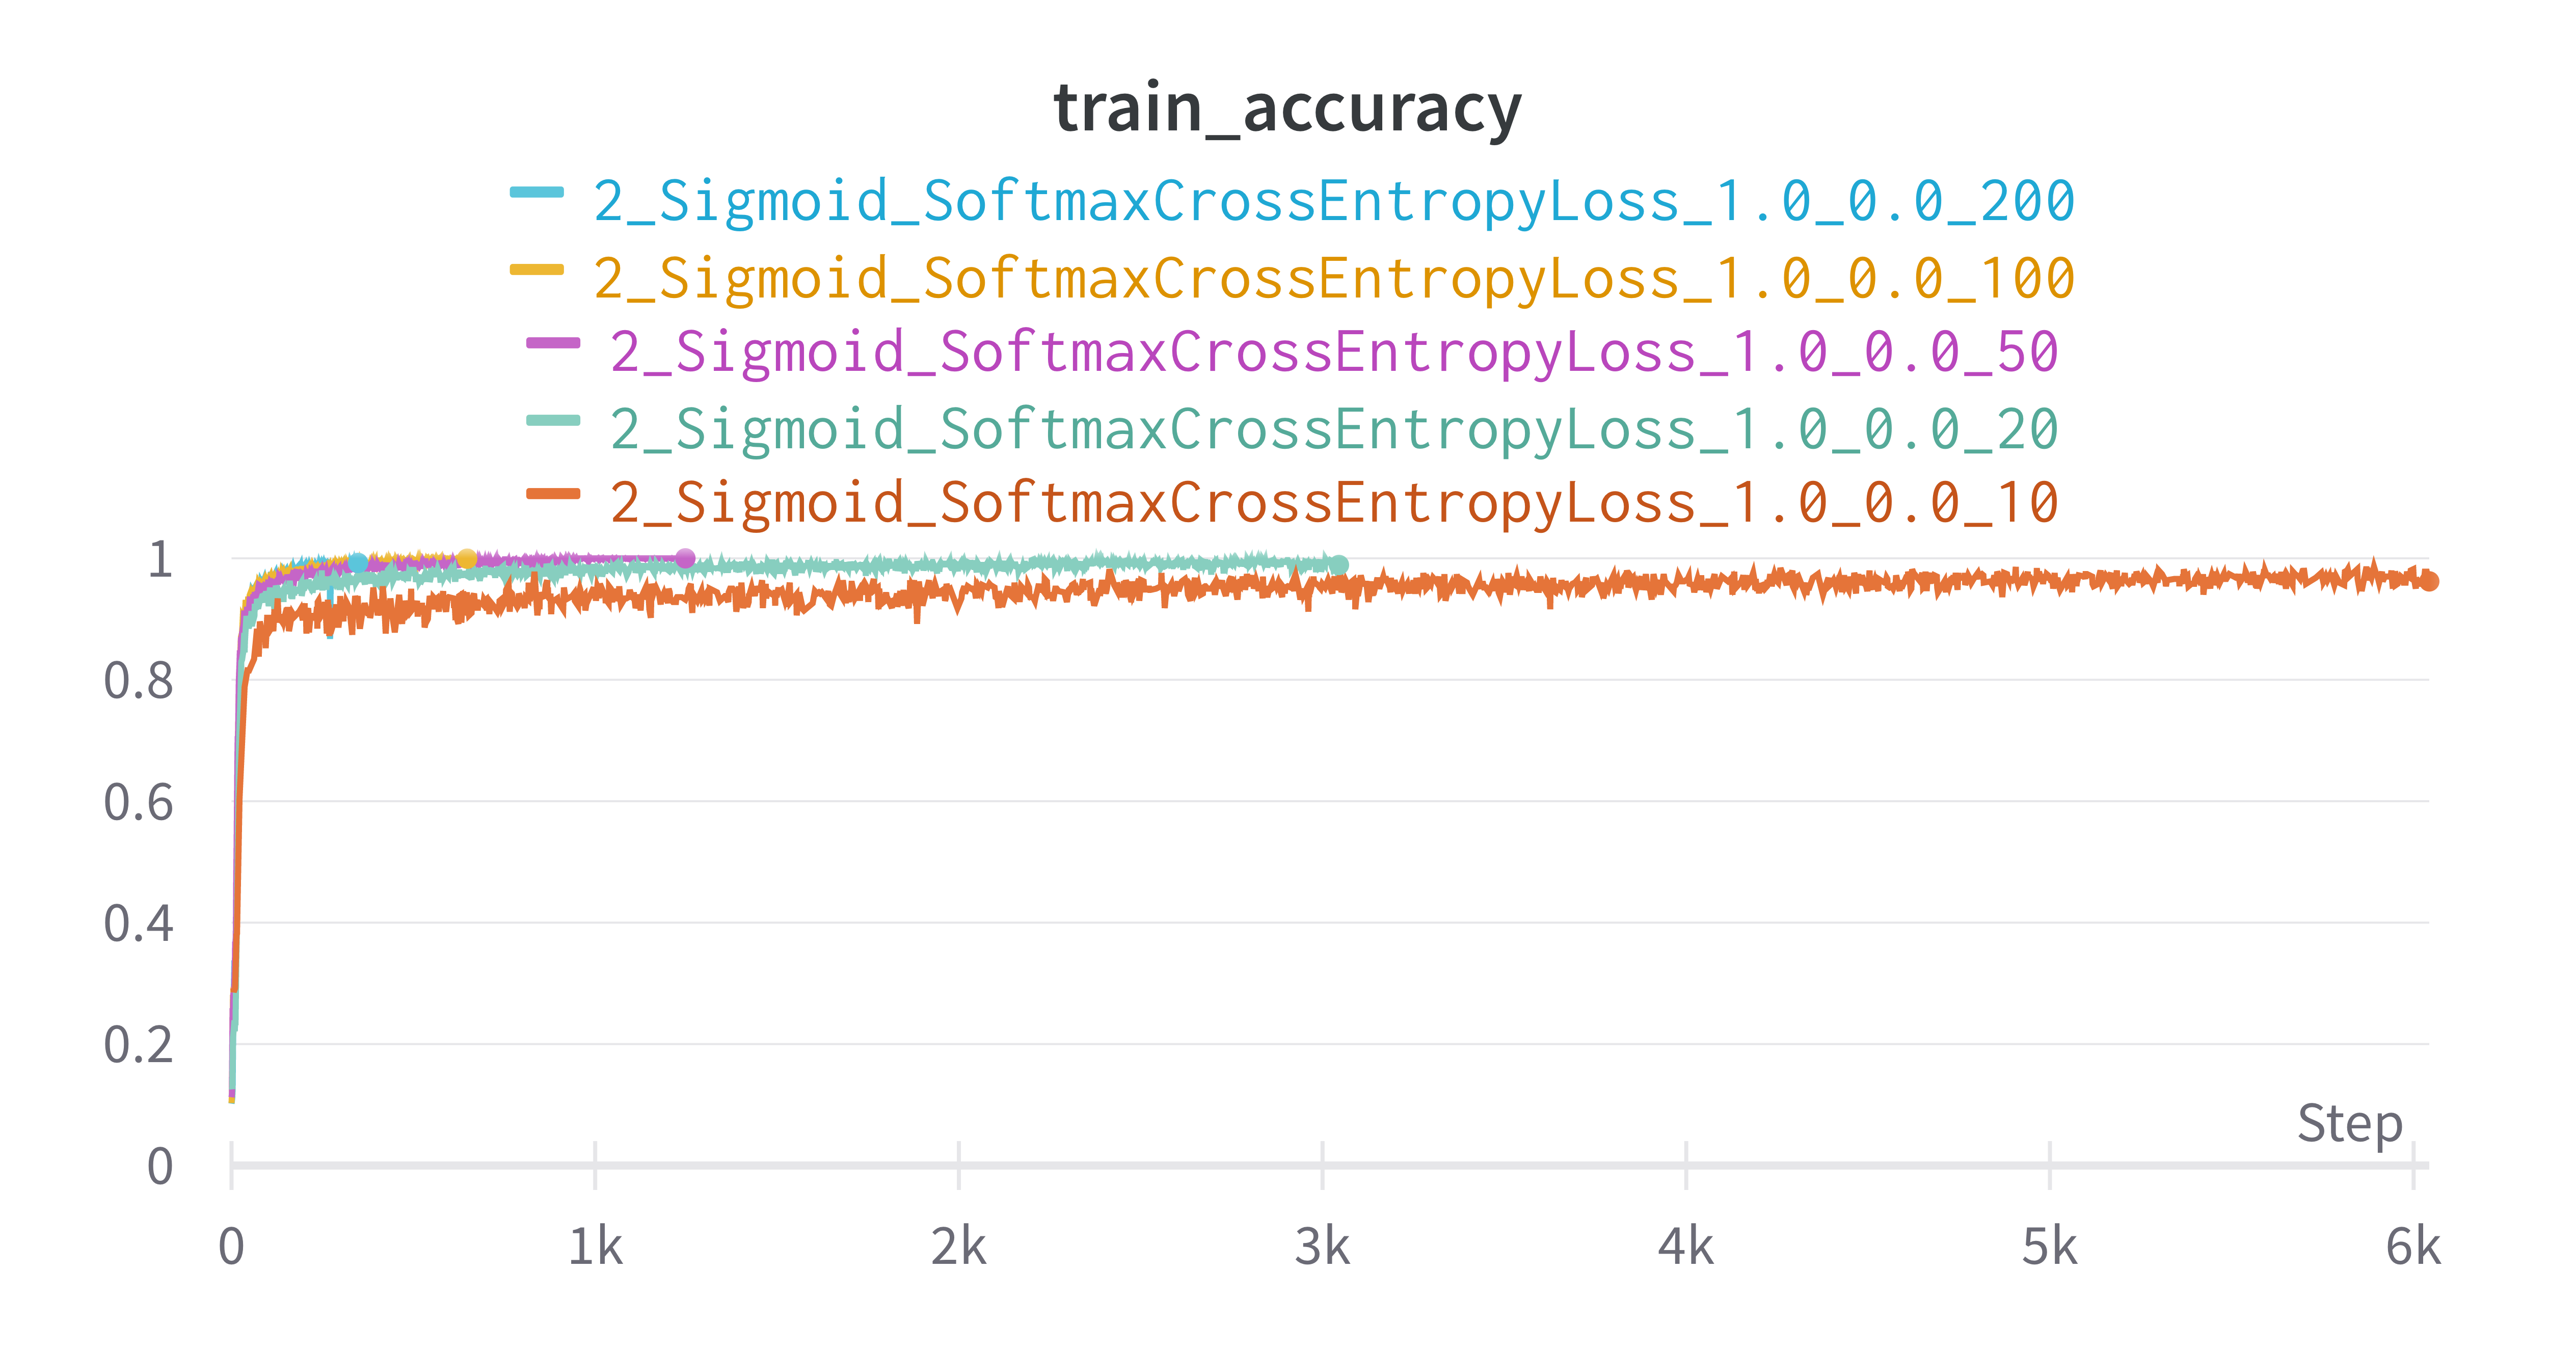
\includegraphics[width=1\textwidth]{../pics/批量大小_2_Sigmoid_Softmax_train_acc.png}
		\caption{2\_Sigmoid\_Softmax 对比 train accuracy}
	\end{subfigure}
	\caption{基于 2\_Sigmoid\_Softmax 调节批量大小}
	\label{fig:12}
\end{figure}

由于选取的模型基本实验结果已经接近完全正确,故而在 50 epoch 下调整批量大小并未发现显著的差距,故而首先选择 1\_Sigmoid\_EuclideanLoss 以 1e-2 为学习率,
放大前 300 step,并且集中对比 10, 200 为批量大小的实验结果;其次选择 2\_Sigmoid\_Softmax 以 1 为学习率,放大前 250 step,并且同样集中对比 10, 200 为批量大小的实验结果。
其结果如图 \ref{fig:13a} 和图 \ref{fig:13b} 所示。

\begin{figure}[htbp]
	\flushleft
	\centering
	\begin{subfigure}{0.475\textwidth}
		\centering
		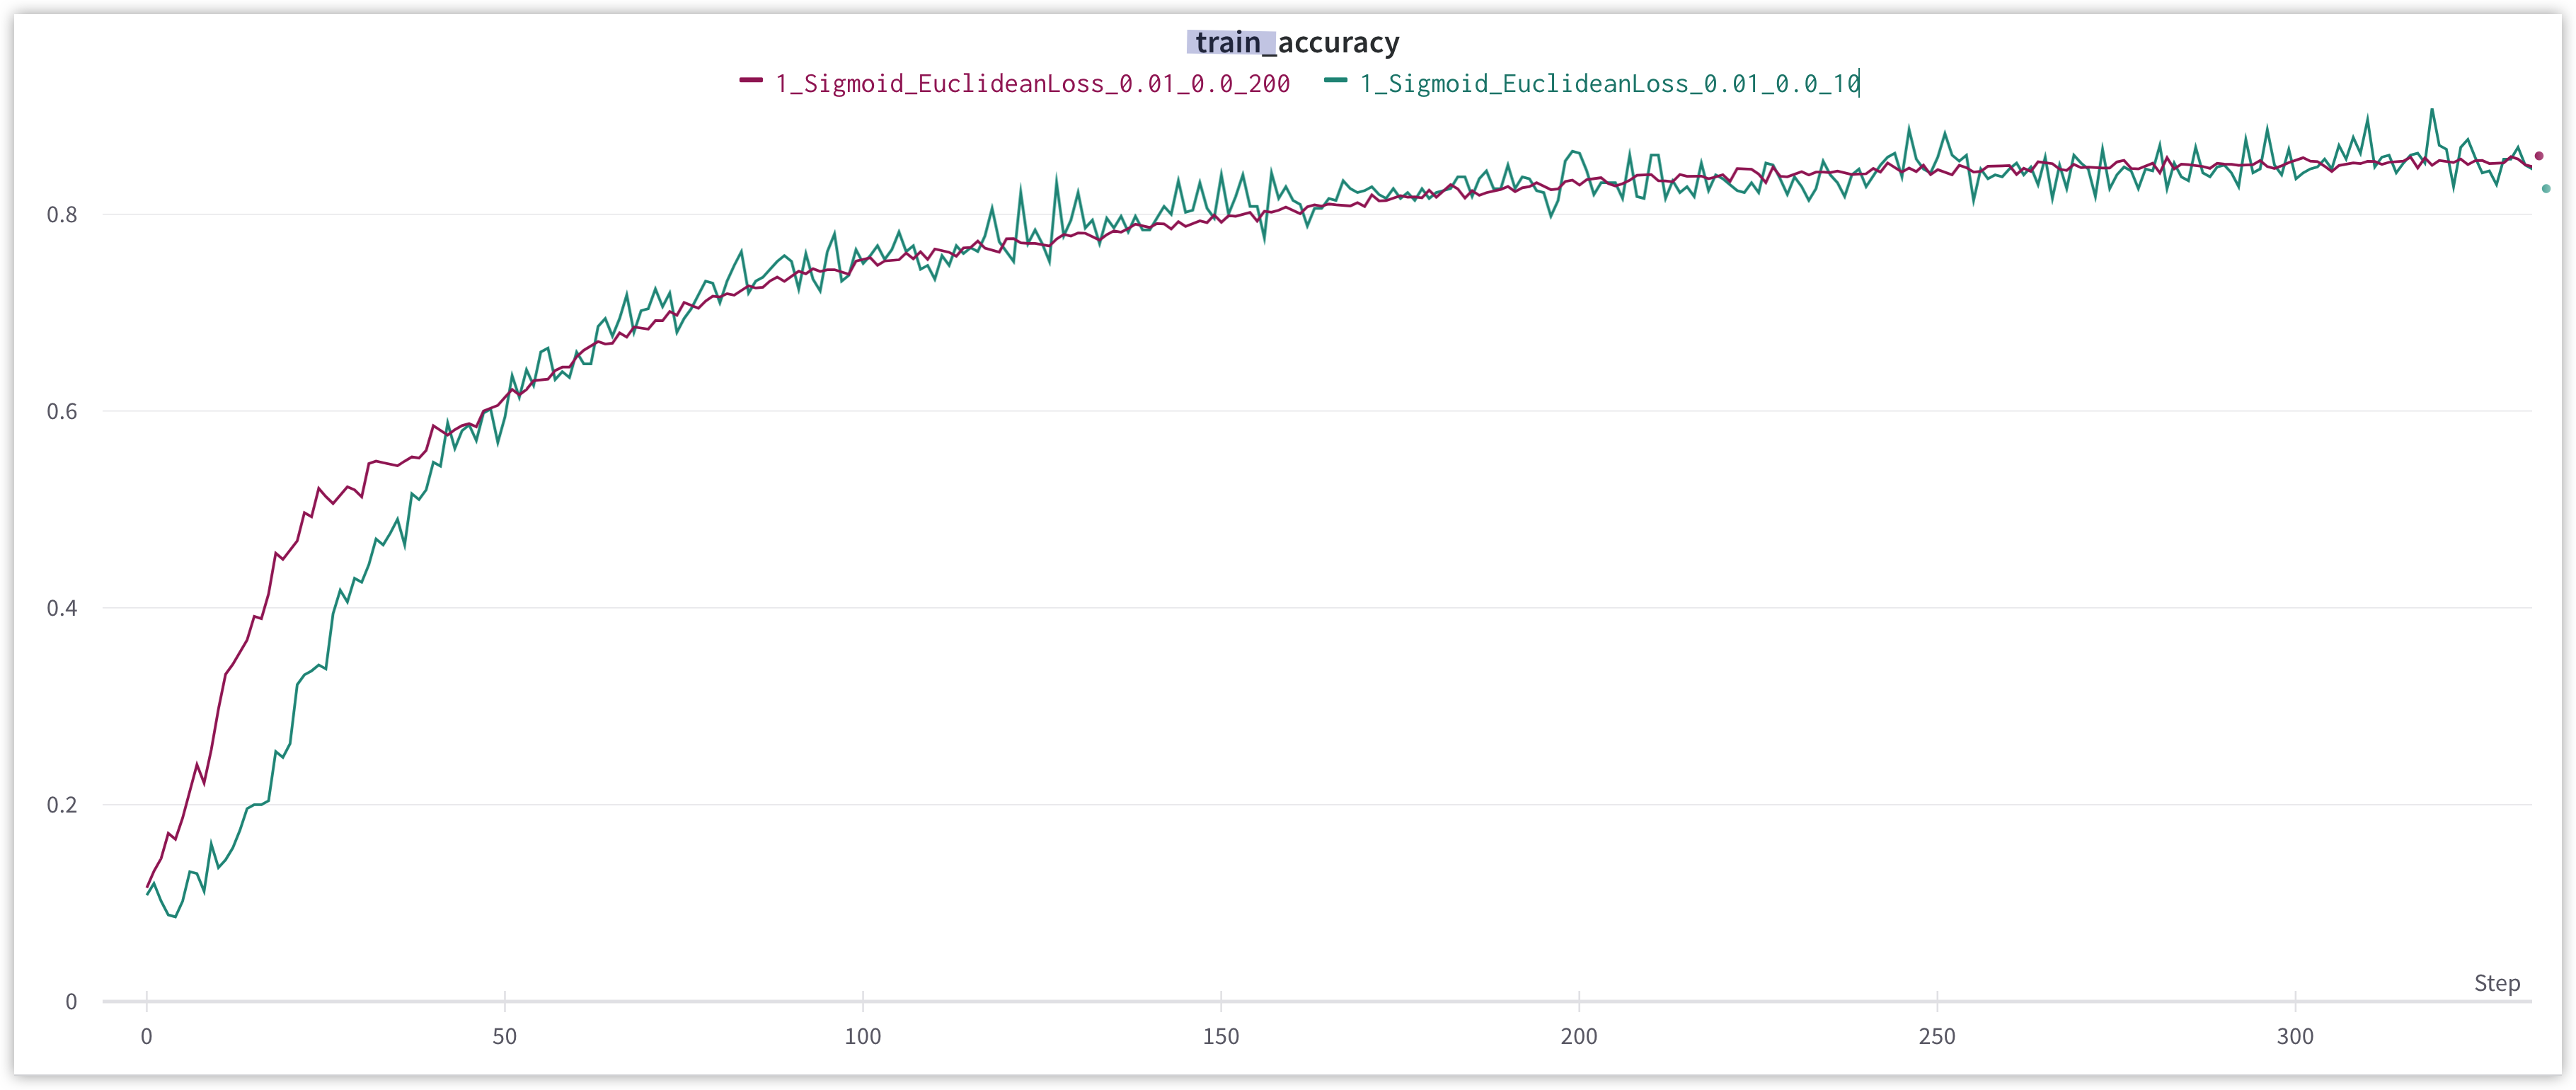
\includegraphics[width=1\textwidth]{../pics/学习率放大1.jpg}
		\caption{放大前 300 step,观察 1\_Sigmoid\_Euclidean 模型}
		\label{fig:13a}
	\end{subfigure}
	\begin{subfigure}{0.475\textwidth}
		\centering
		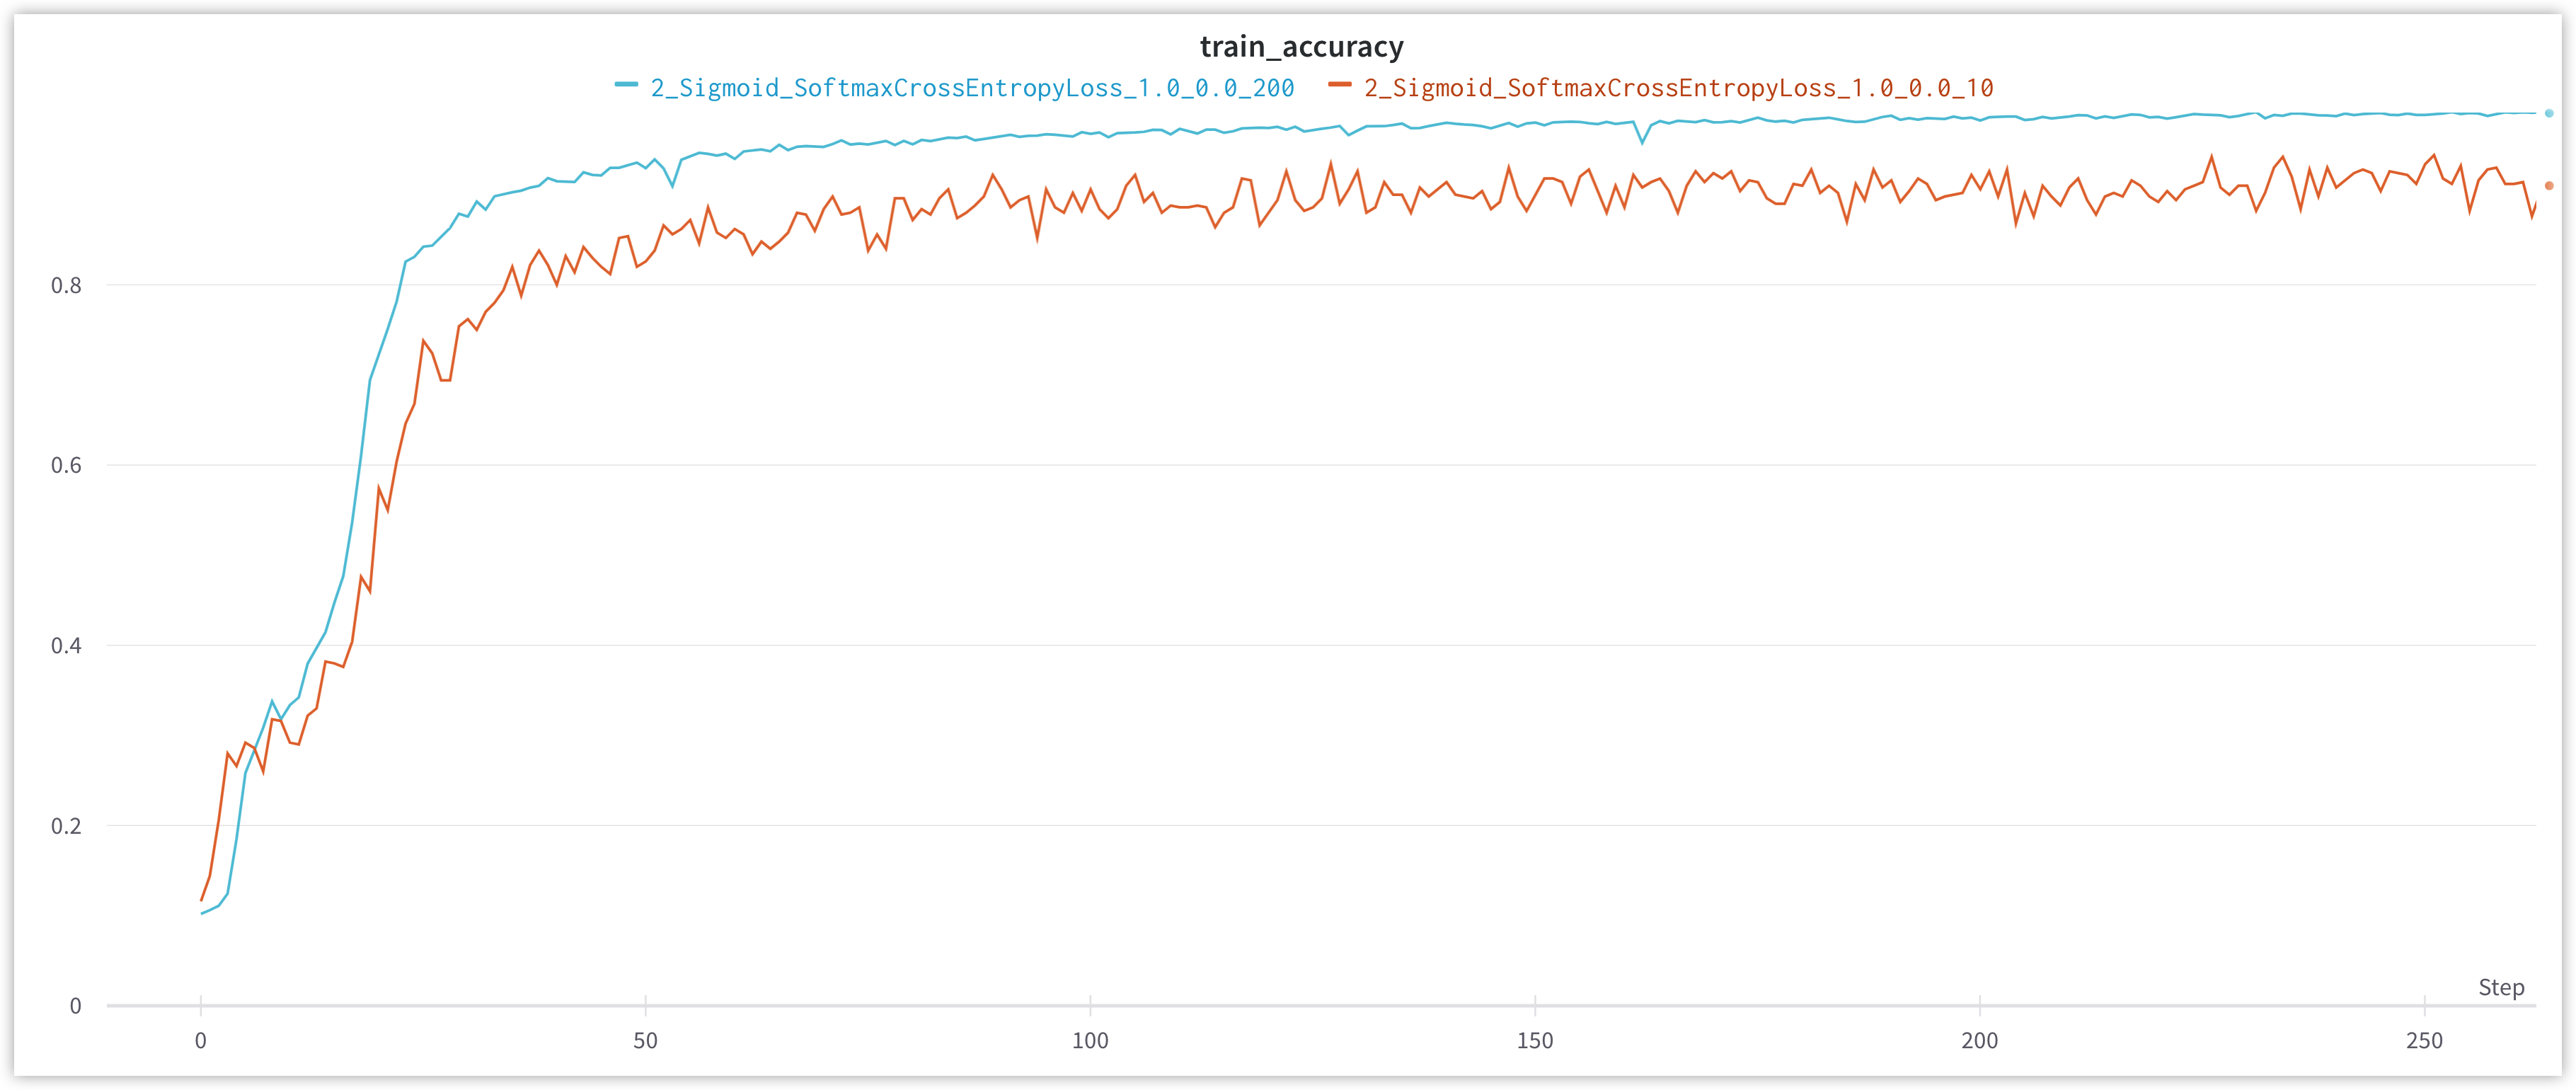
\includegraphics[width=1\textwidth]{../pics/学习率放大2.jpg}
		\caption{放大前 250 step,观察 2\_Sigmoid\_Softmax 模型}
		\label{fig:13b}
	\end{subfigure}
	\caption{放大调节批量大小的前 300 step 和 250 step 并进行对比}
	\label{fig:13}
\end{figure}

一般而言,batch size 越大,批次越少,训练时间会更快一点,但可能造成数据的大量浪费;而 batch size 越小,对数据的利用越充分,浪费的数据量越少,但批次较大,训练会更耗时。
如两图所示,batch size 更大时,能够考虑到更全局的信息,训练过程更加稳定,学习效果的波动更小;而较小的 batch size 梯度更新的频率更高,更容易引入样本噪声,训练效果相应波动性更大。不过,
较小的 batch size 引入样本噪声并不一定绝对有害,实际上在 Gau-GAN 的训练过程中,小的 batch size 提升了生成器的泛化效果。\\
最后参考 batch size 对于训练时间的影响。2\_Sigmoid\_SoftmaxCrossEntropyLoss\_1.0\_0.0\_200 用时 40s,而 2\_Sigmoid\_SoftmaxCrossEntropyLoss\_1.0\_0.0\_10 用时 3m 11s;
1\_Sigmoid\_EuclideanLoss\_0.01\_0.0\_10 用时 2m 14s,而 1\_Sigmoid\_EuclideanLoss\_0.01\_0.0\_200 用时 29s,符合之前的预期。
\end{document}